% Dokument
\documentclass{article}

\usepackage[dvips=false,pdftex=false,vtex=false,left=1.2cm,right=1.2cm,
top=0.4cm,bottom=0.5cm,includeheadfoot,
paperwidth=148mm,paperheight=210mm,twoside]{geometry}

% Schnittmarken, auskommentieren für randlose Version
\usepackage[cam,a4,center,dvips]{crop}

% Songspackage
\usepackage[chorded, noshading]{songs}										

% Umlaute
\usepackage[ngerman]{babel}											
\usepackage[utf8]{inputenc}		

\usepackage{pdfpages}
\usepackage{watermark}
\usepackage{multicol}

%Kein Einzug bei Absatz-Beginn
\setlength{\parindent}{0in} 			

% Helvetica
\usepackage[T1]{fontenc}
\usepackage[scaled]{helvet}

%Überschriften zentrieren
\usepackage[center]{titlesec}

% Header und Footer
\usepackage{fancyhdr}
\pagestyle{fancy}	

\fancyhead{} % clear all header fields	
\fancyfoot{} % clear all footer fields				

% Seitenzahl bei geraden/linken Seiten nach links/aussen
% Seitenzahl bei ungeraden/rechten Seiten nach rechts/aussen
\fancyfoot[LE,RO]{\thepage}

% Pfadiralala Oben Innen
\fancyhead[LO,RE]{Pfadiralala IV}

\renewcommand{\sectionmark}[1]{}
\newcommand{\mymarks}{%
\ifthenelse{\equal{\leftmark}{\rightmark}}
{\rightmark}
{From \rightmark\ until \leftmark}}
\fancyhead[LE,RO]{\mymarks}

%Inhaltsverzeichnisse
\newindex{titelIndex}{titelIndexF}
% Seitennummer anstatt Liednummer
\indexsongsas{titelIndex}{\thepage}
 
% Seiten
\songcolumns{1}

% Hintergrundbild
\usepackage{wallpaper}

% Balken Refrain
\setlength{\cbarwidth}{0pt}
% Balken Liedanfang und Ende											
\setlength{\sbarheight}{0pt}											

% Nummerierung
\nosongnumbers

% Lieder 
\renewcommand*\familydefault{\sfdefault}
% Überschriften
\renewcommand{\stitlefont}{\sffamily\bf\LARGE\centering}
% Strophen
\renewcommand{\lyricfont}{\sffamily}
% Akkorde
\renewcommand{\printchord}[1]{\sffamily\bf#1}
% Refrain
%\renewcommand{\chorusfont}{\it}
\renewcommand{\everychorus}{\textnote{\bf Refrain}}
% Beschreibungen
%\renewcommand{\scripturefont}{\sffamily\it}
% Inhaltsverzeichnis
\renewcommand{\idxtitlefont}{\sffamily} 
\renewcommand{\idxlyricfont}{\sffamily}

% Kein Autor unter Titel
\renewcommand{\extendprelude}{
}

% Worte und Weise
 \newcommand{\wuweise}{}
 \newsongkey{wuw}{\def\wuweise{}}
                 {\def\wuweise{\normalsize\bf Worte und Weise: #1\par}}

% Melodie
 \newcommand{\melodie}{}
 \newsongkey{mel}{\def\melodie{}}
                 {\def\melodie{\normalsize\bf Melodie: #1 }}

% Text
 \newcommand{\text}{}
 \newsongkey{txt}{\def\text{}}
                 {\def\text{\normalsize\bf Text: #1\par}}

% Bock
 \newcommand{\bock}{}
 \newsongkey{bo}{\def\bock{}}
                 {\def\bock{\normalsize\it Liederbock: #1  }}

% Pfadiralala II
 \newcommand{\pfadii}{}
 \newsongkey{pfii}{\def\pfadii{}}
                 {\def\pfadii{\normalsize\it Pfadiralala II: #1 }}

% Pfadiralala III
 \newcommand{\pfadiii}{}
 \newsongkey{pfiii}{\def\pfadiii{}}
                 {\def\pfadiii{\normalsize\it Pfadiralala III: #1 }}

% Jurtenburg
 \newcommand{\jurte}{}
 \newsongkey{ju}{\def\jurte{}}
                 {\def\jurte{\normalsize\it Jurtenburg: #1}}


 %Nach dem Lied
 \renewcommand{\extendpostlude}{
 \wuweise\melodie\text\bock\pfadii\pfadiii\jurte\break
 }

% Notennamen
%\notenamesin{A}{B}{C}{D}{E}{F}{G}
%\notenamesout{A}{H}{C}{D}{E}{F}{G}

%mit oder ohne Bilder kompilieren
\newboolean{pics} %Deklaration
\setboolean{pics}{true}

\begin{document}
\begin{songs}{titelIndex}

\section*{Impressum}

\vspace{10pt} Das „Pfadiralala IV“ ist das Liederbuch der Region Kurhessen im Verband Christlicher Pfadfinderinnen und Pfadfinder. Es ist ausschließlich zum internen Gebrauch von den Mitgliedern der Region bestimmt und wird nur an diese ausgegeben. Das Liederbuch stellt daher keine Veröffentlichung im Sinne des Pressegesetzes dar. Alle Rechte an den Melodien, Texten und Zeichnungen liegen bei den Autoren. \\ \vspace{10pt} 

\begin{centering}
\begin{multicols}{2}

\subsection*{Redaktion}
Laurenz Mäthrich \\ Rabea-Maria Brandt \\ \textit{Stamm Graf Folke Bernadotte, Fulda} \\ ~\\
Jonas Höchst \\ \textit{Neuanfang Kirchhain} \\

\subsection*{Mitarbeit}
Peter Kurzok \\ \textit{Stamm Mückenstürmer, Bad Hersfeld} \\ ~\\
Jacob Mellin \\ Johanna Mellin \\ Mikesch Türck \\ Sophie Haentjens \\ \textit{Stamm Graf Folke Bernadotte, Fulda} \\

\vfill\null
\columnbreak

\subsection*{Zeichnungen}
Irena Ruppert \\ \textit{Stamm Gottfried von Ebersberg, Hettenhausen} \\ ~\\

Lena Rausch \\ Heiko Schmelz \\ Julian Schomber \\
\textit{Stamm Martin Luther, Lumdatal} \\ ~\\

Julia Adam \\ Anke Witzky \\
\textit{Stamm St. Georg, Hann. Münden}  \\ ~\\

Mikesch Türck \\ \textit{Stamm Graf Folke Bernadotte, Fulda} \\ ~\\

Juliane Hartung \\ \textit{Stamm Diemelfüchse, Trendelburg} \\ ~\\

VCP Hessen

\end{multicols}

\subsection*{}
\vspace{6em} \copyright~2021 VCP Kurhessen \\
2. Auflage, 200 Exemplare

\end{centering}

 \newpage
\section*{Vorwort}

\begin{flushright} 
Kurhessen, 18. September 2012
\end{flushright}

Liebe Pfadfinder, Ranger/Rover und Wölflinge! \\ 

Nach über einem Jahr Arbeit - von den ersten Entwürfen zum Abtippen der Lieder, vom Setzen der Noten bis zum Korrektursingen, von den Zusatzinformationen bis hin zum Vervollständigen des Layouts \& Designs - haben wir das Werk, das ihr in euren Händen haltet, fertiggestellt. Wir sind uns sicher, dass noch diverse Rechtschreibfehler und vielleicht sogar Fehler in den Noten zu finden sind. Das bitten wir zu entschuldigen und freuen uns auf das erste Team, das fehlerlos arbeitet. \\ 

Vielen Dank an alle, die uns an diversen Regionsveranstaltungen bei der Auswahl der Lieder, beim Durchsingen und mit ihren kreativen Kunstwerken unterstützt haben. Ein großer Dank gilt auch denen, die die deutsche Rechtschreibung in all ihren Details beherrschen und uns auf allerlei Fehler aufmerksam gemacht haben. \\

Wir hoffen, die in der Region gesungenen Lieder möglichst gut abgebildet zu haben und wünschen euch viel Spaß beim Gebrauch des Buches! \\ 

Gut Pfad.

\begin{flushright} 
Kurhessen, \today
\end{flushright}

Als vor fast zehn Jahren die erste Auflage des Pfadiralala IV herausgekommen ist, war an eine Neuauflage natürlich noch nicht zu denken. Mit dem Pfadiralala IVplus als Ergänzungsband mit ganz vielen neuen Liedern und immer noch vorhandenen Nachfrage nach dem Pfadiralala IV hat sich die RV II / 2019 entschieden, eine neue Auflage zu produzieren. \\

Die Probesingen in Bad Hersfelder Kellern und bei der ersten RV in Niestetal wurden durch die Coronapandemie unterbrochen. Das Ziel, das Buch zum Landeslager 2020 herauszubringen, wurde gleich mit dem ganzen Landeslager um ein Jahr verschoben. \\

Jetzt ist es soweit und es gibt eine neue Auflage mit viel weniger Fehlern und mindestens genauso vielen Liedern für euch! \\

Gut Pfad, \\
das Pfadiralala-Team \newpage

\showindex[2]{Inhaltsverzeichnis}{titelIndex}

\thiswatermark{}
\songsection{Traditionelles}

\ifthenelse{\boolean{pics}}{
\vspace{40pt}
\centering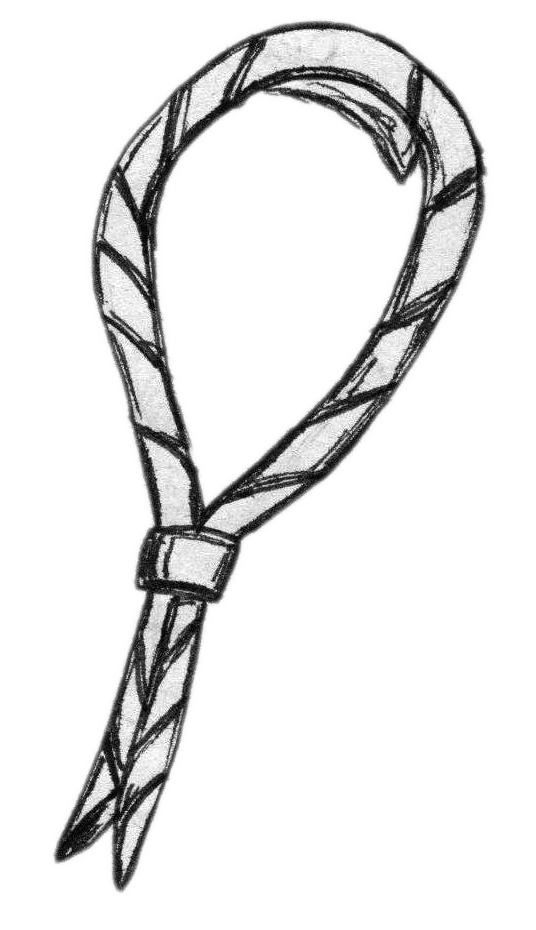
\includegraphics[width=0.7\textwidth]{Bilder/traditionelles_heiko.png}
}{}
\newpage

\leftwatermark{\put(-48,-586){
\includegraphics{Daumenregister/DaumenregisterA_A}}}
\rightwatermark{\put(351,-585){
\includegraphics{Daumenregister/DaumenregisterAL_A}}}

%\setcounter{page}{3}

\beginsong{Abend ward}[wuw={Rudolf Alexander Schröder, Friedrich Samuel Rothenberg, 1942}, bo={4}, pfiii={73}]

\markboth{\songtitle}{\songtitle}

\beginverse
\endverse
\centering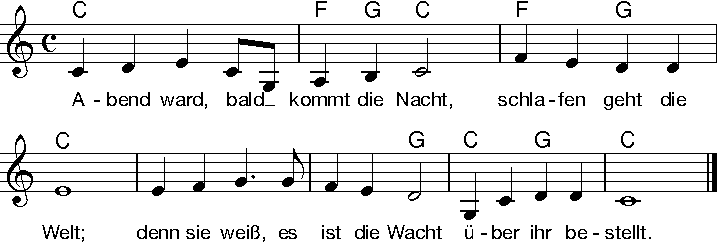
\includegraphics[width=1\textwidth]{Noten/Lied001.pdf}	


\beginverse
\[C]Einer wacht und \[F]trägt \[G]all\[C]ein
\[F]ihre \[G]Müh' und \[C]Plag',
der lässt keinen einsam \[G]sein, 
\[C]weder \[G]Nacht noch \[C]Tag.
\endverse 

\beginverse
^Jesus Christ, mein ^Hort ^und ^Halt,
^dein ge^denk' ich ^nun,
tu mit Bitten dir Ge^walt, 
^bleib bei ^meinem ^Ruhm.
\endverse

\beginverse
^Wenn Dein Aug' ob ^mei^nem ^wacht,
^wenn Dein ^Trost mir ^frommt,
weiß ich, dass auf gute ^Nacht 
^guter ^Morgen ^kommt.
\endverse

\endsong
\beginscripture{}
%nix g'fund'n

\endscripture

\begin{intersong}

\end{intersong}
\beginsong{Abends treten Elche}[wuw={Heinrich Eichen, Gerd Lascheit, 1931}, bo={3}, pfii={6}, pfiii={33}]

\markboth{\songtitle}{\songtitle} 

\beginverse
\endverse

\centering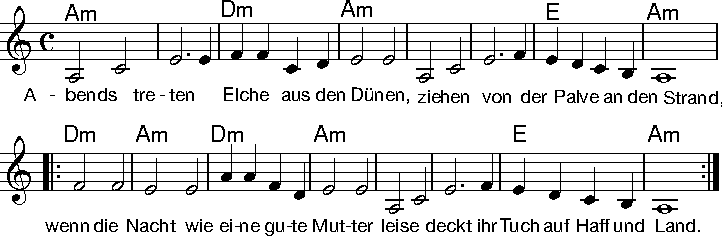
\includegraphics[width=1\textwidth]{Noten/Lied002.pdf}

\beginverse
\[Am]Ruhig trinken \[Dm]sie vom großen \[Am]Wasser, 
darin Sterne \[E]wie am Himmel \[Am]steh'n.
\lrep \[Dm]Und sie heben ihre starken \[Am]Köpfe 
lautlos in des \[E]Sommerwindes \[Am]Weh'n. \rrep
\endverse

\beginverse
^Langsam schreiten ^wieder sie von ^dannen, 
Tiere einer ^längst vergang'^nen Zeit. 
\lrep ^Und sie schwinden in der Ferne ^Nebel 
wie im hohen ^Tor der Ewig^keit. \rrep
\endverse


\endsong
\beginscripture{}
Das Lied war in der ostpreußischen Bevölkerung - auch nach der Flucht vieler vor der Roten Armee 1945 in den Westen des Reiches - sehr beliebt.
\endscripture

\begin{intersong}

\end{intersong}
\beginsong{Allzeit Bereit}[mel={Hermann Mettel, 1927}, txt={Johann Heinrich Lützel, 1934}, bo={14}, pfii={1}, pfiii={2}]

\markboth{\songtitle}{\songtitle}

\beginverse 
\endverse  

\centering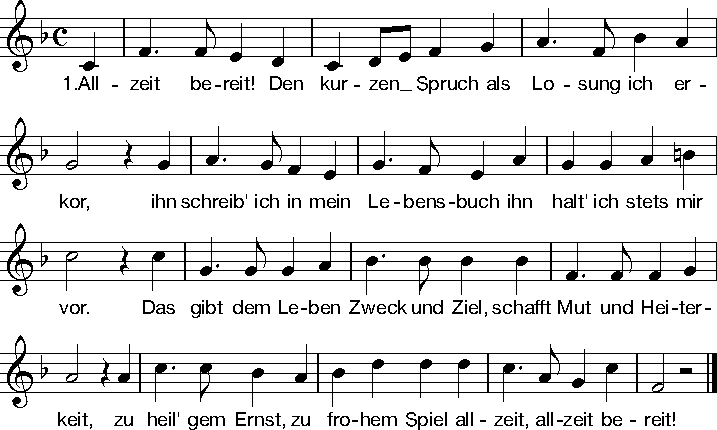
\includegraphics[width=1\textwidth]{Noten/Lied003.pdf}	

\beginverse
Allzeit bereit, dem zu entflieh'n, was mir das Herz befleckt.
Nichts schlechtes soll mich abwärts zieh'n, hoch ist mein Ziel gesteckt.
Gott zum lebend'gen Eigentum sei Leib und Seel' geweiht,
zu seines Namens Ehr' und Ruhm: Allzeit, allzeit bereit!
\endverse

\beginverse
Allzeit bereit, wahr sei der Mund, unwandelbar die Treu'.
Rein sei das Herz, fest sei der Bund, der Wandel ohne Scheu.
So hilf mir Gott, du starker Hort, dass ich kann jederzeit
erfüllen treu das Losungswort: Allzeit, allzeit bereit!
\endverse


\endsong

\beginscripture{}
Bundeslied des VCP, der CPD und anderer christlicher Pfadfinderbünde.
\endscripture

\begin{intersong}

\end{intersong}
\beginsong{And're, die das Land so sehr nicht liebten}[txt={Theodor Kramer 1938}, mel={Erich Schmeckenbecher,	 1979}, bo={30}, pfii={84}]

\markboth{\songtitle}{\songtitle}

\beginverse
\endverse
 

\centering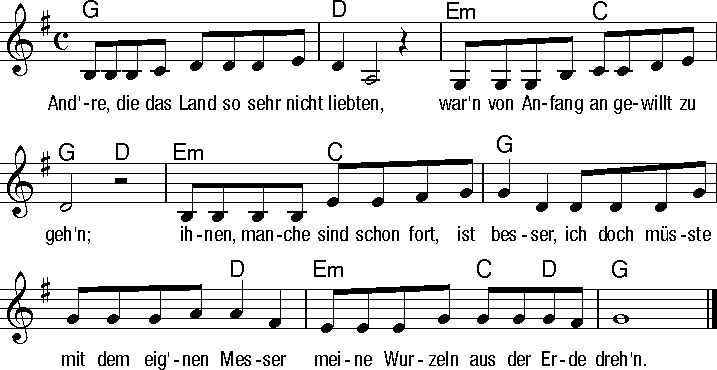
\includegraphics[width=1\textwidth]{Noten/Lied005.pdf}	

% 2 Seiten nötig! 

\beginverse
\[G]Keine Nacht hab' ich seither ge\[D]schlafen, 
\[Em]und es ist mir \[C]mehr als weh zu\[G]mut.\[D]
\[Em]Viele Wochen \[C]sind seither ver\[G]strichen, 
alle Kraft ist längst aus mir ge\[D]wichen,
\[Em]und ich fühl', dass \[C]ich dar\[D]an ver\[G]blut'.
\endverse

\beginverse
^Und doch müsst' ich mich von hinnen ^heben, 
^sei's auch nur zu ^bleiben, was ich ^war.^
^Nimmer kann ich, ^wo ich bin, ge^deihen, 
draußen braucht ich wahrlich nicht zu ^schreien,
^denn mein leises ^Wort war ^immer ^wahr.
\endverse

\beginverse
^Seiner wär' ich wie in alten ^Tagen 
^sicher, schluchzend ^wider mich ge^wandt. ^
^Hätt' ich Tag und ^Nacht mich nur zu ^heißen, 
mich samt meinen Wurzeln auszu^reißen
^und zu setzen ^in ein ^and'res ^Land. 
\endverse

\endsong

\beginscripture{}
Kramer beschäftigte sich hauptsächlich mit gesellschaftlichen Außenseitern und verfasste so über 10.000 Werke, von denen viele unveröffentlicht sind. Dieses Lied fand jedoch Einzug in das Fahrtenbuch der Wandervögel "Der Zupfgeigenhansel".
\endscripture

\begin{intersong}

\ifthenelse{\boolean{pics}}{
\ThisLRCornerWallPaper{1}{Bilder/andrediedasland_irena3.png}
}{}

\end{intersong} % 005 <-> 004, um platz zu sparen!
\beginsong{Am Ural}[wuw={axi (Alexej Stachowitsch)}, bo={18}, pfii={46}]

\markboth{\songtitle}{\songtitle}

\beginverse
\endverse 

\centering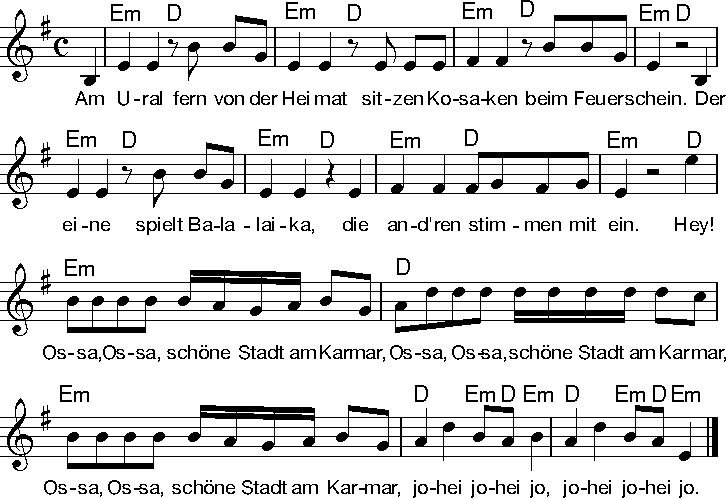
\includegraphics[width=1\textwidth]{Noten/Lied004.pdf}	

\beginverse
Am \[Em]Himmel, \[D]da leuchten die \[Em]Sterne, \[D] der \[Em]Wolf heult \[D]im finst'ren \[Em]Tal. \[D]
Die \[Em]Heimat, \[D]du grüßt sie von \[Em]Ferne, \[D] ver\[Em]gessen \[D]ist all' ihre \[Em]Qual! \[D]Hey!
\endverse

\beginchorus
\[Em]Ossa, Ossa, schöne Stadt am Karmar, \[D]Ossa, Ossa, schöne Stadt am Karmar,
\[Em]Ossa, Ossa, schöne Stadt am Karmar, \lrep \[D]Jo-hei, \[Em]jo-\[D]hei-\[Em]jo! \rrep
\endchorus
 
\beginverse
Die ^Pferde ^hell spitzen die ^Ohren, ^wenn die Ko^saken ^jauchzen und ^schrein. ^
Sie ^geben ^den Pferden die ^Sporen ^drüben am ^Wasser ^im Feuer^schein. ^Hey!
\endverse

\endsong
%\beginscripture{}
%Kosaken = Gemeinschaften freier Reiterverbände, zu denen sich flüchtige Russen und Ukrainer, manchmal auch nur Abenteurer %oder anderweitig Abtrünnige, in den südlichen Steppengebieten zusammenschlossen.
%\endscripture

\begin{intersong}

\end{intersong}
\beginsong{An den sechs vergang'nen Tagen}[wuw={Alf Zschiesche}, bo={26}, pfii={28}, pfiii={55}]

\markboth{\songtitle}{\songtitle}

\beginverse
\endverse

\centering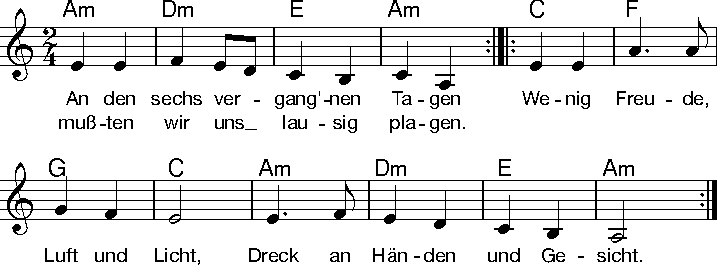
\includegraphics[width=1\textwidth]{Noten/Lied102.pdf}

\beginverse
\[Am]Heute \[Dm]hat die \[E]Welt uns \[Am]wieder, Klampfen\[Dm]spiel und \[E]hundert \[Am]Lieder,
\lrep \[C]wandern \[F]durch die \[G]Wälder \[C]mit \[Am]zu dem \[Dm]Sieben\[E]meilen\[Am]schritt. \rrep
\endverse

\beginverse
^Und so ^geht es ^immer ^munter Berge ^rauf und ^wieder ^runter,
\lrep ^alle ^uns're ^Müdig^keit ^steckt zu^haus im ^Arbeits^kleid. \rrep
\endverse

\beginverse 
^Sieben ^Tage ^hat die ^Woche, sechse ^sind wir ^rumge^krochen,
\lrep ^doch am ^siebten ^lebt sich's ^flott, ^also ^will's der ^liebe ^Gott. \rrep
\endverse

\endsong

%\beginscripture
%\endscripture

\begin{intersong}

\end{intersong}
\beginsong{Auf vielen Straßen}[txt={Björn Behnke}, mel={Alf Zschiesche, 1950}, bo={34}]

\markboth{\songtitle}{\songtitle}
 
\beginverse
\endverse

\centering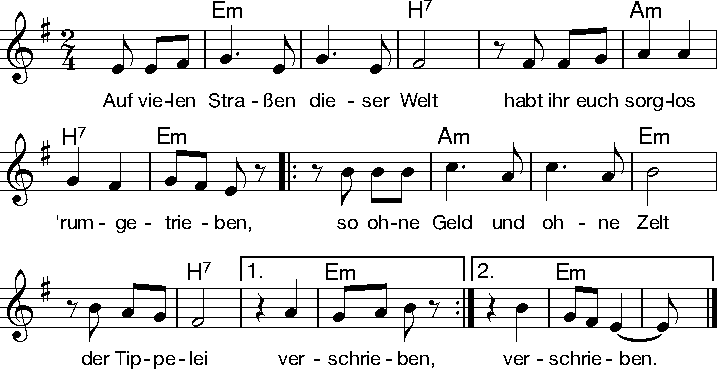
\includegraphics[width=1\textwidth]{Noten/Lied006.pdf}	

\beginverse
Was galt euch \[Em]Armut, was Ge\[H7]fahr?
Ihr habt ver\[Am]achtet \[H7]und zer\[Em]schunden,
\lrep da draußen \[Am]treibend Jahr für \[Em]Jahr
doch euer \[H7]Glück ge\[Em]funden. \rrep
\endverse

\beginverse
Habt manches ^Lied der Einsam^keit
wohl in die ^Nacht hin^aus ge^sungen.
\lrep Auf fremden ^Meeren, fern der ^Zeit,
ist euer ^Sang ver^klungen. \rrep
\endverse


\endsong

\beginscripture{}
\newpage
\endscripture 

\begin{intersong}
\ifthenelse{\boolean{pics}}{
\vspace{30pt}
\centering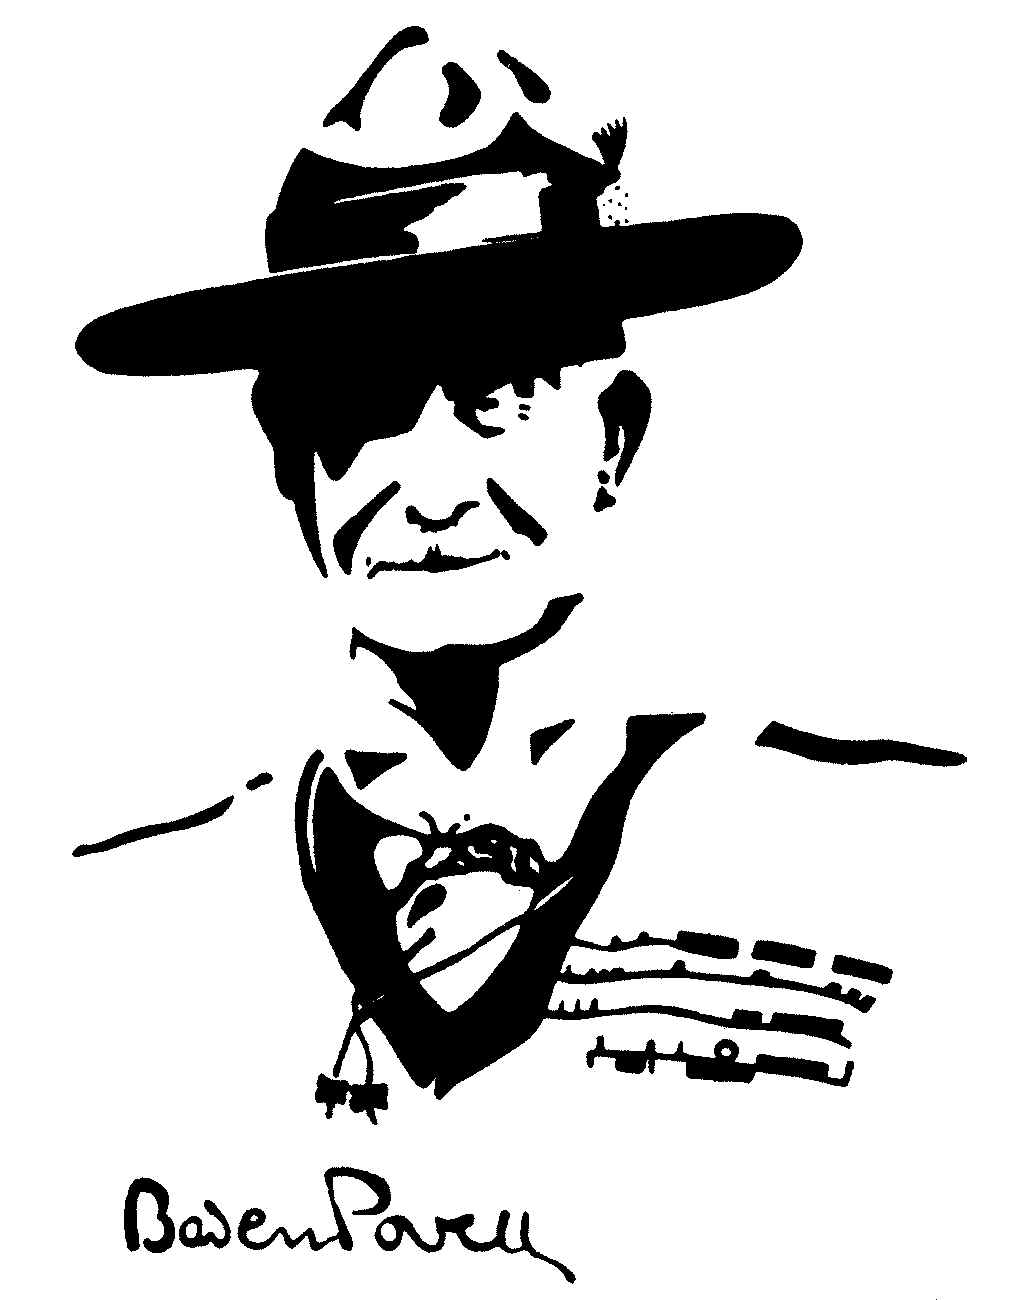
\includegraphics[width=1\textwidth]{Bilder/powell.jpg}
}{}

\end{intersong}

\leftwatermark{\put(-48,-586){
\includegraphics{Daumenregister/DaumenregisterA_B}}}
\rightwatermark{\put(351,-585){
\includegraphics{Daumenregister/DaumenregisterAL_B}}}

\beginsong{Bajuschki baju}[wuw={Michail Jurgewitsch Lermontow, ca. 1840, deutsche Übersetung von J.v. Günther}, pfii={103}, pfiii={39}, index={Schlaf, mein Bub}]

\markboth{\songtitle}{\songtitle}

\beginverse
\endverse
 
\centering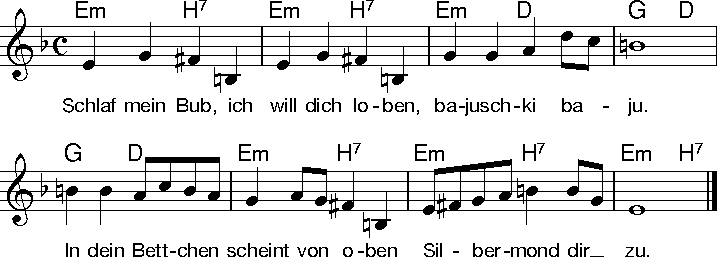
\includegraphics[width=1\textwidth]{Noten/Lied007.pdf}	


\beginverse
\[Em]Durch die \[H7]Felsen, \[Em]durch die \[H7]Lande, \[Em]strömt des \[D]Tereks \[G]Flut. \[D]
\[G]Der Tsche\[D]tschene \[Em]schleicht am \[H7]Strande, \[Em]schleift sein \[H7]Messer \[Em]gut. \[H7]
\endverse

\beginverse
^Doch dein ^Vater ^ist ein ^Reiter, ^greift ihn ^auf im ^Nu!  ^
^Schlaf, mein ^Kind, ^schlaf ruhig ^weiter, ^bajusch^ki ba^ju. ^
\endverse

\beginverse
^Du wächst ^auf, die ^Zeit hat ^Flügel, ^wirst ein ^Held wie ^er;  ^
^Mutig ^steigst du ^in die ^Bügel, ^greifst nach ^dem Ge^wehr. ^
\endverse

\beginverse
^Sticken ^werde ^ich mit ^Seide ^Sattel ^dir und ^Schuh'. ^
^Schlaf mein ^Kindchen, ^meine ^Freude, ^bajusch^ki ba^ju. ^
\endverse

\beginverse
^Ein Ko^sak wirst ^du bei^zeiten ^und ein ^Held ge^nannt; ^
^wirst du ^einstmals ^von mir ^reiten, ^winkst du ^mit der ^Hand. ^ 
\endverse

\beginverse
^Denk, stehst ^du im ^Kampfes^feuer, ^meiner ^immer^zu. ^
^Schlaf mein ^Liebling, ^mir so ^teuer, ^bajusch^ki ba^ju. ^ \[Em]
\endverse

\endsong

\beginscripture{}
''Bajuschki baju'' ist russisch und bedeutet "Heia heia". Das Lied entstand zur Zeit des Kaukasuskrieges (1817 - 1864), in dem das Russische Kaiserreich versuchte, die Kontrolle über den von Tscherkessen und Tschertschenen besetzten Nordkaukasus zu erlangen.
\endscripture

\begin{intersong}
\ifthenelse{\boolean{pics}}{
\ThisLRCornerWallPaper{1}{Bilder/bajuschkibaju_irena.png}
}{}

\end{intersong} 
\beginsong{Banner, Zelte}[wuw={Wolfgang Hartmann, VCP Stamm Franken, 1980er Jahre}, pfii={80}, pfiii={37}]

\markboth{\songtitle}{\songtitle}

\beginverse  
\endverse

\centering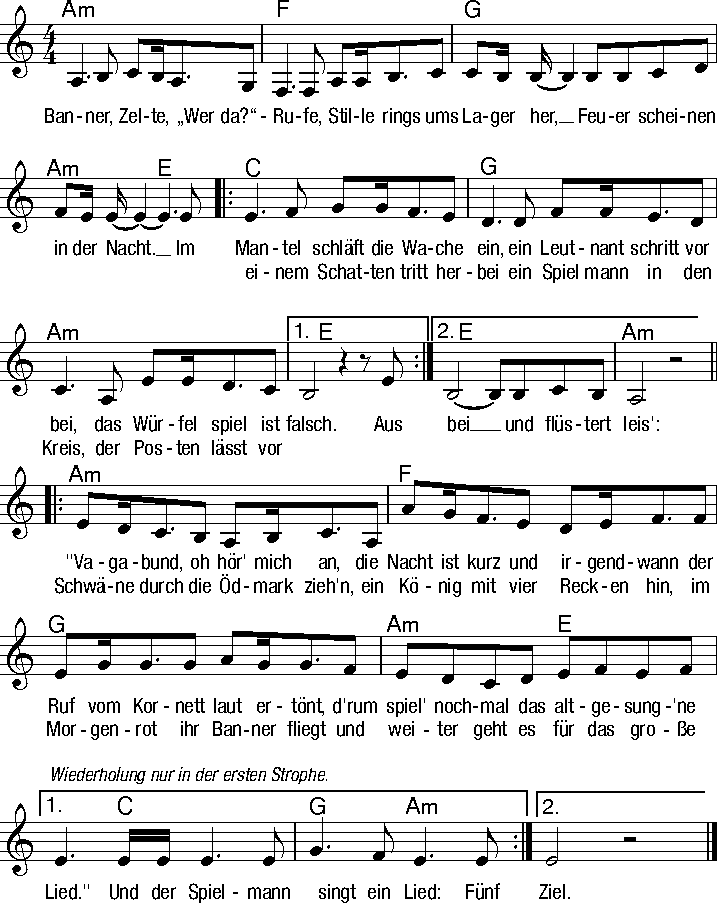
\includegraphics[width=1\textwidth]{Noten/Lied008.pdf}

\beginverse
\[Am]Im Feindeslager hört man's \[F]auch, durch Stille säuselt \[G]Melodie,
Herzen lauschen \[Am]wie noch nie. \[E]
Die \[C]Klampfe in der Hand, der \[G]Spielmann singt allein und 
\[Am]alles lauscht in dieser \[E]Nacht.
Doch \[C]plötzlich hinter sich hört \[G]er wie vereint den \[Am]Chor 
und alle stimmen \[E]ein in diese Melo\[Am]dei:
\endverse	

\beginchorus
'Fünf \[Am]Schwäne durch die Ödmark zieh'n, ein \[F]König mit vier Recken hin.
Im \[G]Morgenrot ihr Banner fliegt und \[Am]weiter geht es \[E]für das gute Ziel.'

Und \[Am]als der Morgen hell erstrahlt, die \[F]Schlacht beginnt, die Trommel warnt.
Vor\[G]ne steht ein Grenadier, er \[Am]denkt zurück und \[E]legt nieder das Schwert.
\endchorus
 
\beginverse
Und ^als drei Jahr' vergangen ^war'n, das Feld liegt öd und ^leer vorweg
und nichts erinnert ^mehr daran, ^
an ^eine nicht gewes'ne Sch^lacht, doch plötzlich hört man ^leis'
der Nachtigallen ^Schlag.
Als ^ob eine fremde Melo^die zög über das ^Land,
von Ferne weht ein ^Wind und trägt sie ^fort.
\endverse

\beginchorus
'Fünf Schwäne durch die Ödmark zieh'n, ein \[F]König mit vier Recken hin.
Im \[G]Morgenrot ihr Banner fliegt und \[Am]weiter geht es \[E]für das gute Ziel.' \[Am]
\endchorus

\endsong

%\beginscripture{}

%\endscripture

\begin{intersong}

\end{intersong}
\beginsong{Bella ciao}[wuw={nach einem italienischen Partisanenlied 1942, Übersetzung: Diether Dehm}, bo={33}, pfii={102}, index={An ihrer Schulter}]

\markboth{\songtitle}{\songtitle}

\beginverse
\endverse

\centering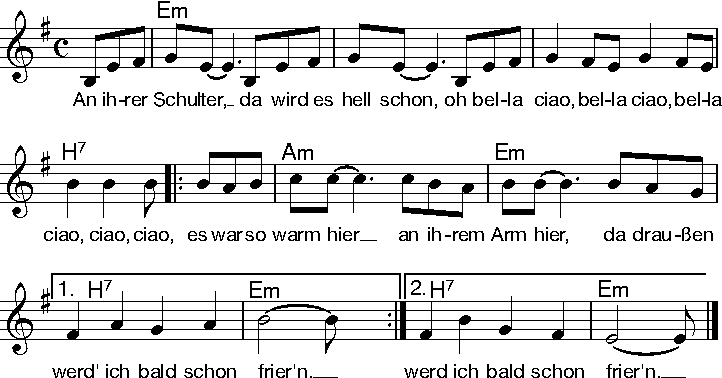
\includegraphics[width=1\textwidth]{Noten/Lied010.pdf}	

\beginverse
Kann nicht gut \[Em]schießen und krieg' schnell Angst auch,
o bella ciao, bella ciao, bella \[H7]ciao, ciao, ciao.
\lrep Soll ich ein \[Am]Held sein, dem das ge\[Em]fällt? Nein!
Verfluchter \[H7]Krieg, verfluchter \[Em]Feind! \rrep
\endverse
 
\beginverse
Sah Blut an ^Hütten, sah Frauen bitten,
o bella ciao, bella ciao, bella ^ciao, ciao, ciao.
\lrep Den kleinen ^Luca, der 14 ^Jahr' war,
ich hab zu ^lang nur zuge^seh'n. \rrep
\endverse

\beginverse
Ihr in den ^Bergen, heut' komm ich zu euch,
o bella ciao, bella ciao, bella ^ciao, ciao, ciao.
\lrep Was kein Kom^mando und kein Be^fehl kann:
Ich werde ^heute Parti^san. \rrep
\endverse

\beginverse
Wenn ich am ^Dorfplatz mal tot herumlieg',
o bella ciao, bella ciao, bella ^ciao, ciao, ciao,
\lrep dann sagt der ^Priester statt langer ^Predigt:
'Nie mehr Fa^schismus, nie mehr ^Krieg!' \rrep
\endverse

\beginverse
Nur noch der ^Kuss hier, kommt einer nach mir,
o bella ciao, bella ciao, bella ^ciao, ciao, ciao.
\lrep Dem wünsch' ich ^Zeiten, wo man so ^eine
wie dich nicht ^mehr verlassen ^muss. \rrep
\endverse

\endsong

\beginscripture{}
Diese Version des antifaschistischen Arbeiterliedes glorifiziert im Gegensatz zur anderen nicht den "Heldentod" der Partisanen.
\endscripture

\begin{intersong}

\end{intersong}
\beginsong{Bella ciao}[wuw={nach einem italienischen Partisanenlied 1942, Übersetzung: Horst Berner}, pfii={101}, pfiii={30}, index={Eines Morgens, in aller Frühe}]

\markboth{\songtitle}{\songtitle}

\beginverse
Eines \[Em]Morgens, in aller Frühe,
o bella ciao, bella ciao, bella \[H7]ciao, ciao, ciao,
\lrep eines \[Am]Morgens, in aller \[Em]Frühe
trafen \[H7]wir auf unser’n \[Em]Feind. \rrep 
\endverse

%\centering\includegraphics[width=1\textwidth]{Noten/Lied009.pdf}	

\beginverse
Parti\[Em]sanen, kommt, nehmt mich mit euch,
o bella ciao, bella ciao, bella \[H7]ciao, ciao, ciao,
\lrep Parti\[Am]sanen, kommt, nehmt mich \[Em]mit euch,
denn ich \[H7]fühl', der Tod ist ^nah. \rrep
\endverse

\beginverse
Wenn ich ^sterbe, oh ihr Genossen,
o bella ciao, bella ciao, bella ^ciao, ciao, ciao,
\lrep wenn ich ^sterbe, oh ihr Ge^nossen,
Bringt mich ^dann zur letzten ^Ruh'. \rrep
\endverse

\beginverse
In den ^Schatten der kleinen Blume,
o bella ciao, bella ciao, bella ^ciao, ciao, ciao,
\lrep in den ^Schatten der kleinen ^Blume,
in die ^Berge bringt mich ^dann. \rrep
\endverse

\beginverse
Und die ^Leute, die geh'n vorüber,
o bella ciao, bella ciao, bella ^ciao, ciao, ciao,
\lrep und die ^Leute, die geh'n vo^rüber,
seh'n die ^kleine Blume ^steh'n. \rrep
\endverse

\beginverse
Diese ^Blume, so sagen alle,
o bella ciao, bella ciao, bella ^ciao, ciao, ciao,
\lrep ist die ^Blume des Parti^sanen,
der ^für die Freiheit ^starb. \rrep
\endverse

\endsong

\beginscripture{}
Die Melodie wurde bereits Anfang des 20. Jahrhunderts von italienischen Reispflückerinnen in der Nähe der Stadt Bologna gesungen, die die harte Arbeit unter erbarmungslosen Arbeitgebern beklagten. Nach der antifaschistischen Umdichtung wurde das Lied auch außerhalb Italiens bekannt und häufig übersetzt und wird noch heute von Antifaschisten gesungen.
\endscripture

\begin{intersong}

\end{intersong}
\beginsong{Bündische Vaganten}[wuw={trenk (Alo Hamm), 1952}, bo={178}, pfii={27}, pfiii={58}, index={Hej, wie vorn der Fetzen fliegt}]

\markboth{\songtitle}{\songtitle}

\beginverse
\endverse

\centering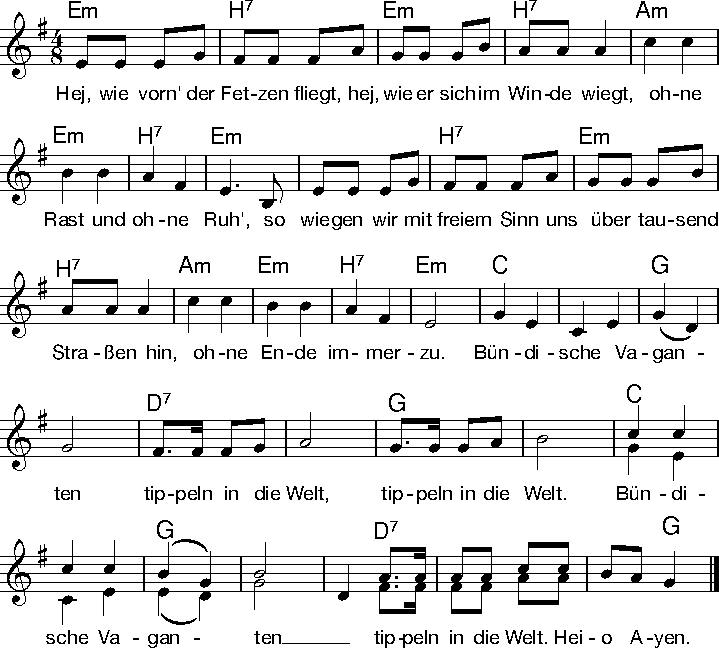
\includegraphics[width=1\textwidth]{Noten/Lied011.pdf}

\beginverse
\[Em]Treiben wir dem \[H7]Süden zu, lässt \[Em]uns der Norden \[H7]keine Ruh',
\[Am]über\[Em]all zu \[H7]Haus' sind \[Em]wir.
Mal \[Em]rüber nach A\[H7]merika, mal \[Em]runter bis nach \[H7]Afrika,
\[Am]hoja, \[Em]hoja, \[H7]das sind \[Em]wir!
\endverse

\beginchorus 
\[C]Bündische Va\[G]ganten
tip\[D7]peln in die Welt, tip\[G]peln in die Welt.
\[C]Bündische Va\[G]ganten 
tip\[D7]peln in die Welt, hei-o A\[G]yen!
\endchorus

\beginverse
^Hast du noch ein ^jung' Gesicht, so ^zage nicht und ^fack'le nicht, 
^frage ^niemals ^nach dem ^'Wie?'
Wer ^nur am Rand der ^Straße klebt, für ^seinen dummen ^Bauch nur lebt,
^misst der ^Ferne ^Zauber ^nie.
\endverse
%\renewcommand{\everychorus}{\textnote{\bf Refrain (wdh.)}}
\beginchorus 
\[C]Bündische Va\[G]ganten
tip\[D7]peln in die Welt, tip\[G]peln in die Welt.
\[C]Bündische Va\[G]ganten
tip\[D7]peln in die Welt, hei-o A\[G]yen!
\endchorus


\endsong

\beginscripture{}
Vagant = Fahrendes Volk/Herumziehender; Das Lied behandelt die deutsche Jugendbewegung zwischen 1919 und 1933, die aus dem Wandervogel entstand und die Hinwendung der städtischen bürgerlichen Jugend zum Naturleben meint.
\endscripture

\begin{intersong}

\end{intersong}
\beginsong{Bürgerlied}[mel={Prinz Eugen, der edle Ritter, ca. 1845}, txt={Adalbert Harnisch, 1845}, index={Ob wir rote, gelbe Kragen}]

\markboth{\songtitle}{\songtitle}

\beginverse 
\endverse

\centering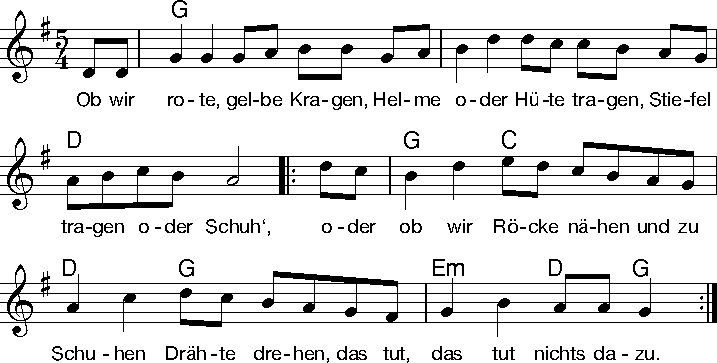
\includegraphics[width=1\textwidth]{Noten/Lied011a.pdf}

\beginverse
Ob wir \[G]können präsidieren
oder müssen Akten schmieren ohne \[D]Rast und ohne Ruh,
ob wir \[G]just Coll\[C]egia lesen 
oder \[D]aber \[G]binden Besen, das tut, \[Em]das tut \[D]nichts da\[G]zu.
\endverse

\beginverse
Ob wir ^stolz zu Rosse reiten, 
oder ob zu Fuß wir schreiten barfuß ^unser'm Ziele zu,
ob uns ^Kreuze ^vorne schmücken 
oder ^Kreuze ^hinten drücken, das tut, ^das tut ^nichts da^zu.
\endverse

\beginverse
Aber ^ob wir Neues bauen 
oder Altes nur verdauen, wie das ^Gras verdaut die Kuh,
ob wir ^in der ^Welt was schaffen 
oder ^nur die ^Welt begaffen, das tut, ^das tut ^was da^zu.
\endverse

\beginverse
Ob wir ^rüstig und geschäftig, 
wo es gilt zu wirken kräftig, immer ^tapfer greifen zu,
oder ^ob wir ^schläfrig denken: 
„Gott wird's ^wohl im ^Schlafe lenken“, das tut, ^das tut ^was da^zu.
\endverse

\beginverse
Ob im ^Kopfe etwas Grütze 
und im Herzen Licht und Hitze, dass es ^brennt in einem Nu,
oder ^ob wir ^hinter Mauern 
immer ^stets im ^Dunkeln kauern: Das tut, ^das tut ^was da^zu.
\endverse

\beginverse
D'rum, ihr ^Bürger, d'rum, 
ihr Brüder, alle eines Bundes Glieder, was auch ^jeder von uns tu'. 
Alle, ^die dies ^Lied gesungen, 
so die ^Alten, ^wie die Jungen: Tun wir, ^tun wir ^was da^zu!
\endverse

\endsong

\beginscripture{}
Das Lied wurde im Mai 1845 für den "Bürgerverein" der Stadt Elging geschrieben, um die Vision eines liberal gesinnten Bürgertums eines einigen deutschen Staates auszudrücken. Das Lied wurde während der Märzrevolution 1848/1849 auf Flugblättern verteilt. Nach der Revolution diente das Lied der neuen Arbeiterbewegung zum Ausdruck ihrer Forderung nach gesellschaftlicher Veränderung.
\endscripture

\begin{intersong}

\end{intersong}
\beginsong{Burschen, Burschen}[wuw={bündische Jugend}, bo={46}, pfii={20}, pfiii={12}]

\markboth{\songtitle}{\songtitle}

\beginverse
\endverse

\centering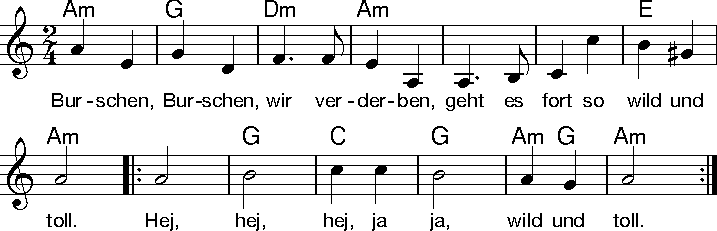
\includegraphics[width=1\textwidth]{Noten/Lied012.pdf}

\beginverse
\[Am]Von den \[G]Füßen \[Dm]weg\[Am]gesoffen 
werden bald die \[E]Stiefel \[Am]sein,
\lrep \[Am]hej, \[G]hej, \[C]hej, ja\[G]ja, \[Am]Stie\[G]fel \[Am]sein. \rrep
\endverse
 
\beginverse
^Eine ^Nacht, ^zwei tol^le Tage 
zechten wir an ^diesem ^Ort,
\lrep ^hej, ^hej, ^hej, ja^ja, ^die^sem ^Ort. \rrep
\endverse

\beginverse
^Zechen ^wir an ^diesem ^Orte, 
hier in diesem ^blauen ^Krug,
\lrep ^hej, ^hej, ^hej, ja^ja, ^blau^en ^Krug. \rrep
\endverse

\beginverse
^Süß das ^Bier und ^weiß ^die Kannen, 
schön die flinke ^Krüger^in.
\lrep ^hej, ^hej, ^hej, ja^ja, ^Krü^ger^in. \rrep
\endverse

\beginverse
^Sauft das ^Bier, zer^schlagt die ^Kannen, 
küsst die schöne ^Krüger^in,
^hej, ^hej, ^hej, ja^ja, ^Krü^ger^in, 
\[Am]hej, \[G]hej, \[C]hej ja\[G]ja, \[Am]bis \[G]sie \[Am]schreit!
\endverse


\endsong

\beginscripture{}
% nix g'fund'n
\endscripture

\begin{intersong}

\ifthenelse{\boolean{pics}}{
\vspace{75pt}
\centering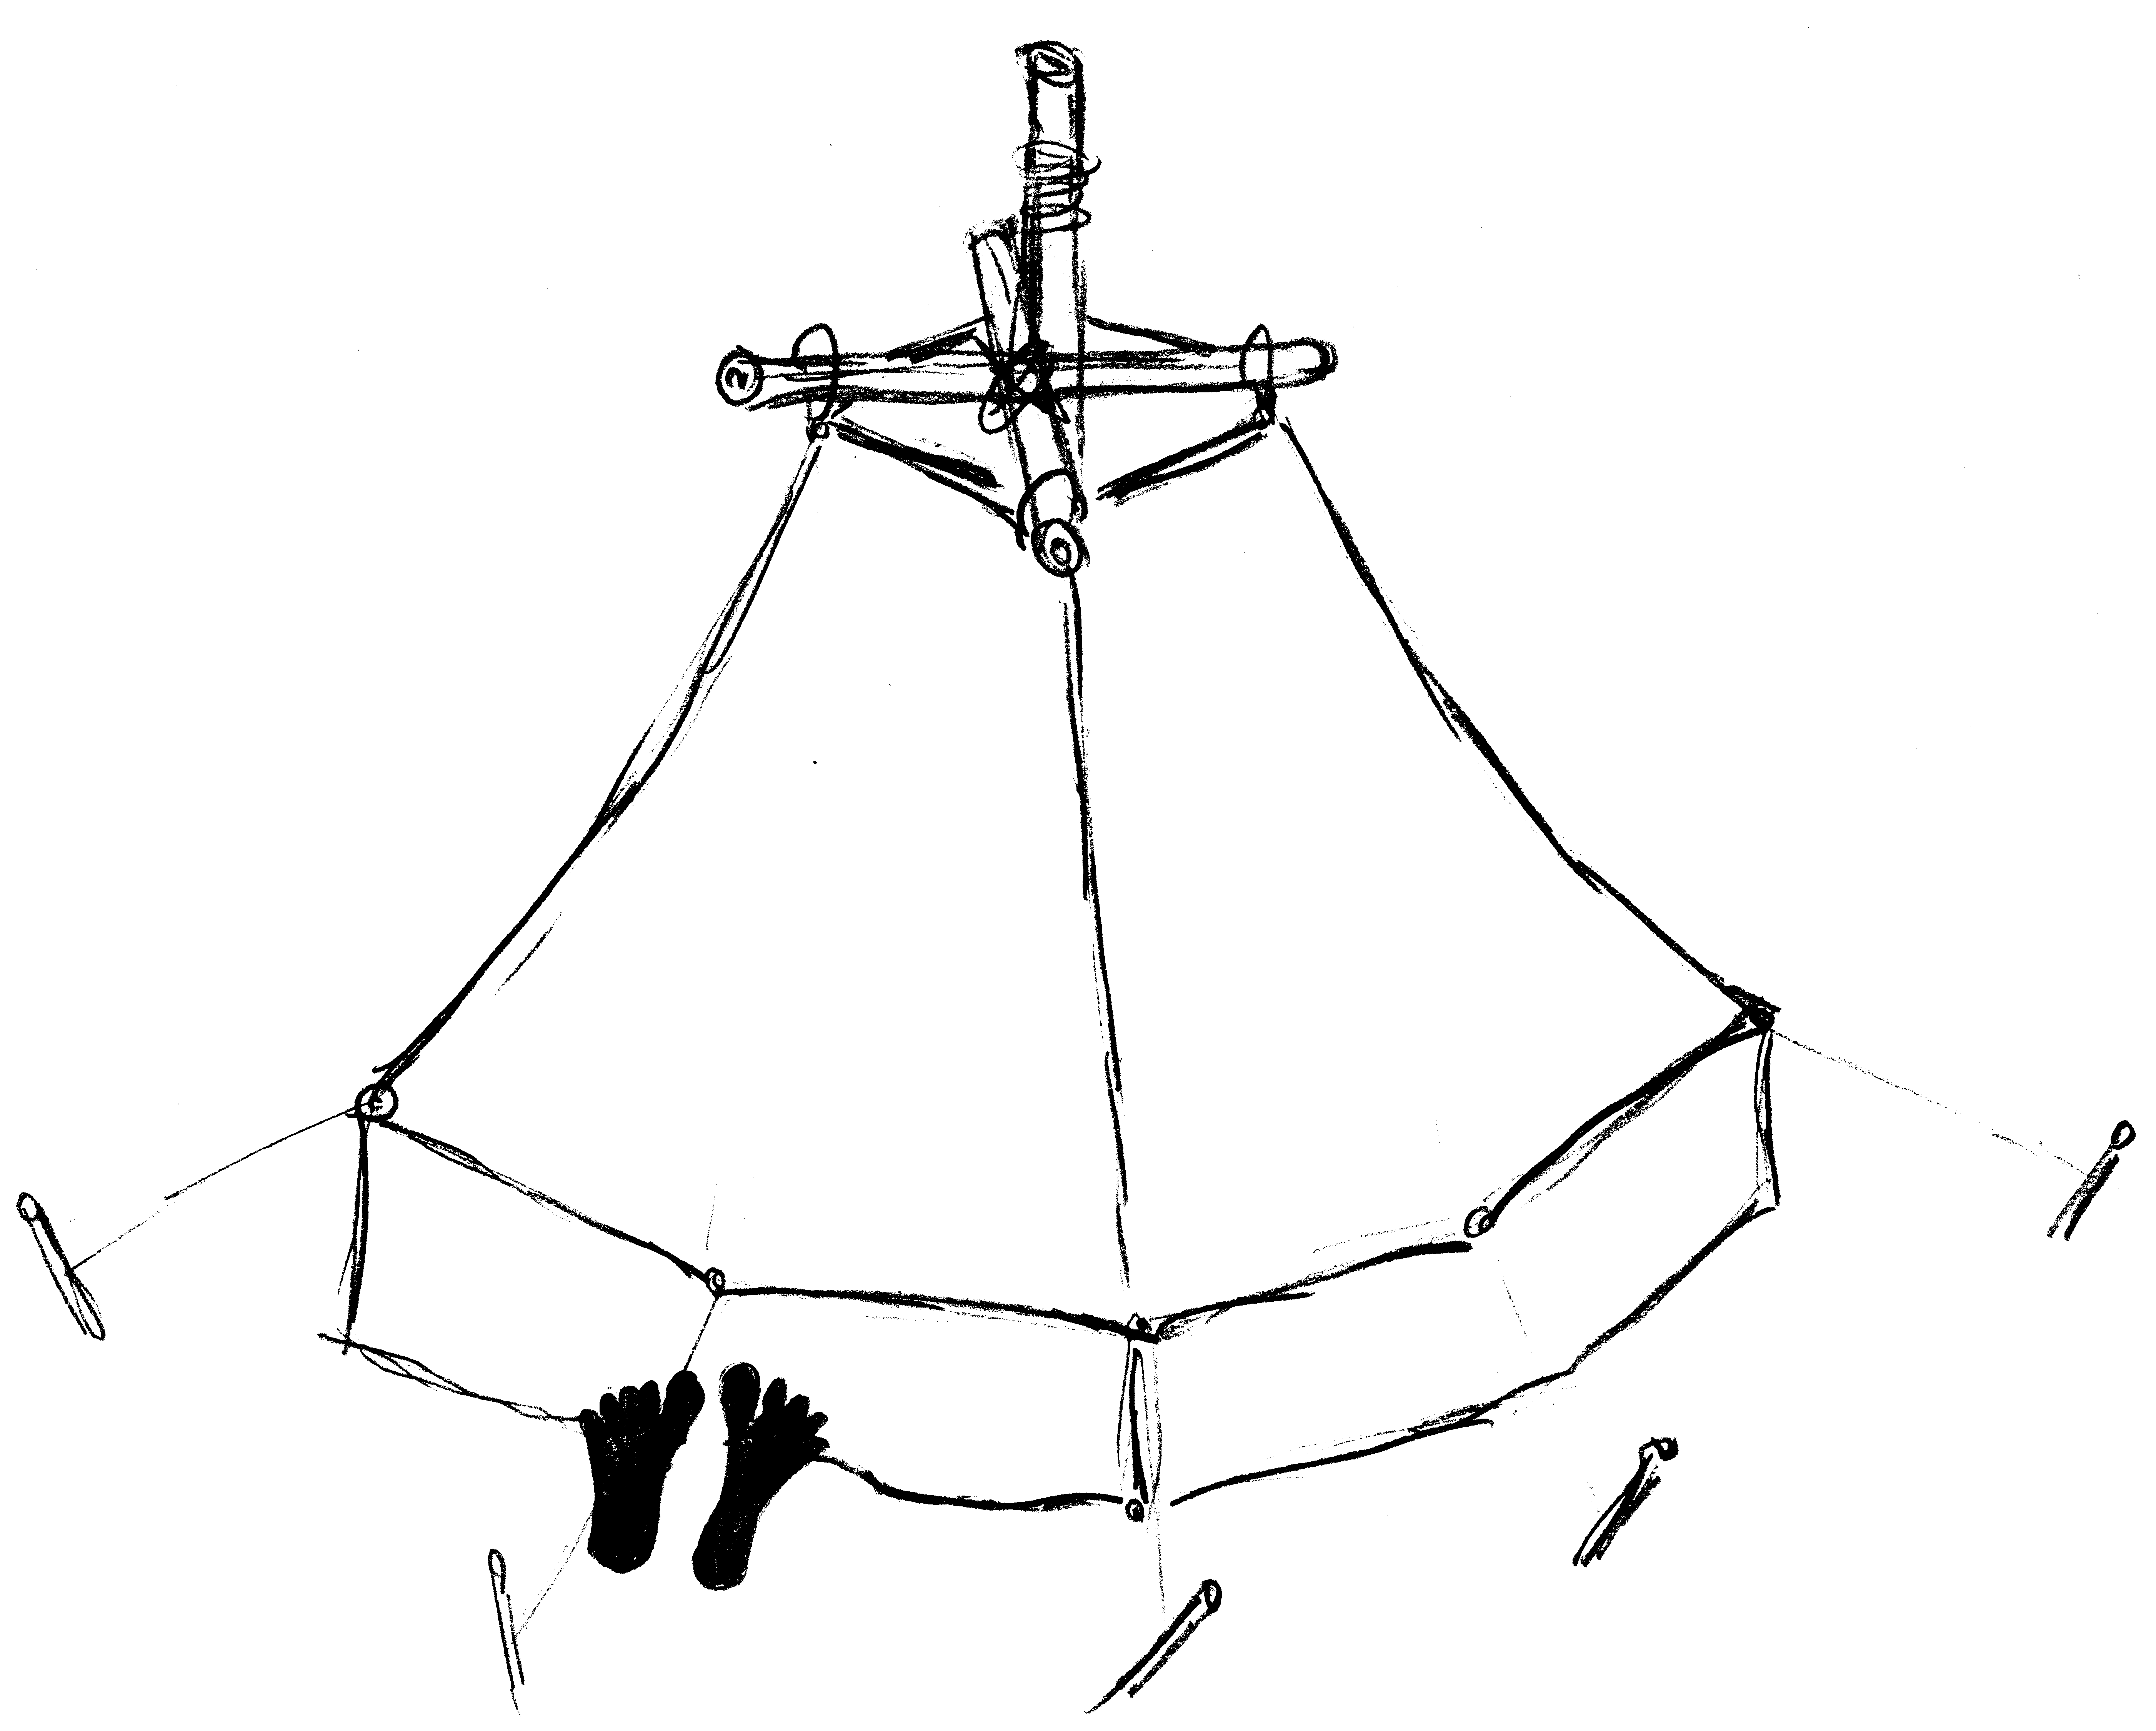
\includegraphics[width=1\textwidth]{Bilder/burschen.png}
}{}

\end{intersong}

\leftwatermark{\put(-48,-586){
\includegraphics{Daumenregister/DaumenregisterA_C}}}
\rightwatermark{\put(351,-585){
\includegraphics{Daumenregister/DaumenregisterAL_C}}}

\beginsong{Circles}[wuw={Gwendolin Lee Zak, 1979, nach einem irischen Volkslied}, bo={204}, pfiii={94}, index={In days gone by}]

\markboth{\songtitle}{\songtitle}

\beginverse
\endverse

\centering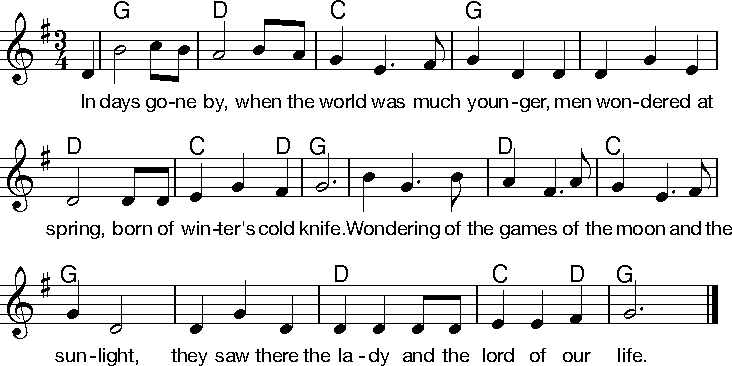
\includegraphics[width=1\textwidth]{Noten/Lied013.pdf}

\beginchorus
\[G]Round and a\[D]round and a\[C]round turns the \[G]good earth;
all things must \[D]change as the \[C]seasons \[D]go \[G]by.
We are the \[D]children of the \[C]Lord and the \[G]Lady,
whose mysteries we \[D]know but we \[C]never \[D]know \[C]why. \[G]
\endchorus 

\beginverse
\[G]In all lands the \[D]people have \[C]tried to the \[G]good earth,
ploughing and \[D]sawing as the \[C]seasons \[D]de\[G]clared,
waiting to \[D]reap of the \[C]rich golden \[G]harvest,
knowing their \[D]joy in the \[C]laughs that \[D]they \[G]shared.
\endverse
\renewcommand{\everychorus}{\textnote{\bf Refrain (wdh.)}}
\beginchorus
\endchorus

\beginverse
^Through Flandern and ^Wales and the ^green land of ^Ireland,
in the kingdoms of ^England and ^Scotland ^and ^Spain
circles grew ^up all a^long the wild ^coastline
and worked for the ^land with the ^sun and ^the ^rain.
\endverse

\beginchorus
\endchorus

\beginverse
^Circles for ^healing and ^working the ^weather,
circles for ^knowing the ^moon and ^the ^sun,
circles for ^thanking the ^Lord and the ^Lady,
circles for ^dancing the ^dance ne^ver ^done.
\endverse

\beginchorus
\endchorus

\endsong

\beginscripture{}
% nix g'fund'n
\endscripture

\begin{intersong}

\end{intersong}

\leftwatermark{\put(-48,-586){
\includegraphics{Daumenregister/DaumenregisterA_D}}}
\rightwatermark{\put(351,-585){
\includegraphics{Daumenregister/DaumenregisterAL_D}}}

\beginsong{Das Gegenlied}[wuw={Claumisch (Michael Schmidt), VCP Bad Hersfeld "Mückenstürmer"}, pfii={180}, pfiii={95}, index={Ich singe hier kein Lied, dass ihr schon kennt}]

\markboth{\songtitle}{\songtitle}

\beginverse
\endverse
\centering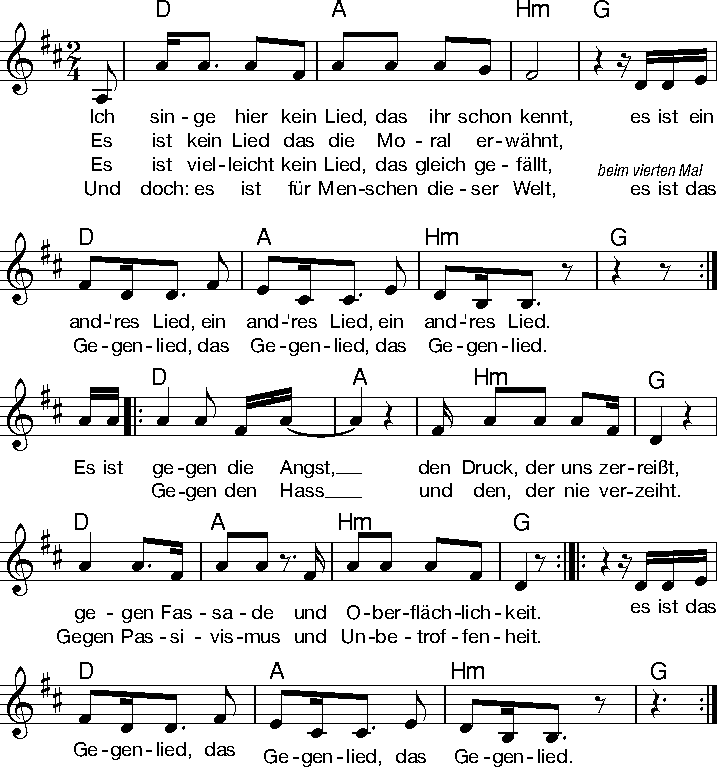
\includegraphics[width=1\textwidth]{Noten/Lied014.pdf}

\beginverse
Es \[D]ist kein Lied, das \[A]irgendwas be\[Hm]weist. \[G]
Es ist ein \[D]and'res Lied, ein \[A]and'res Lied, ein \[Hm]and'res Lied. \[G]
Es \[D]ist auch kein's, das \[A]tiefe Gräben \[Hm]reißt. \[G]
Es ist ein \[D]and'res Lied, ein \[A]and'res Lied, ein \[Hm]and'res Lied. \[G]
Kein \[D]Damokles\[A]schwert, das \[Hm]über uns \[G]schwebt.
Es ist ein \[D]and'res Lied, ein \[A]and'res Lied, ein \[Hm]and'res Lied. \[G]
Wenn \[D]jeder nur ein \[A]bisschen danach \[Hm]lebt, \[G]
es ist ein \[D]Lebenslied, ein \[A]Lebenslied, ein \[Hm]Lebenslied! \[G]
\endverse
 
\beginchorus
Es ist \[D]gegen die \[A]Angst, den \[Hm]Druck der uns zer\[G]reißt,
\[D]gegen Fas\[A]sade und \[Hm]Oberflächlich\[G]keit,
\[D]gegen den \[A]Hass und \[Hm]den der nie ver\[G]zeiht,
\[D]gegen Passi\[A]vismus und \[Hm]Unbetroffen\[G]heit.
\lrep Es ist das \[D]Gegenlied, das \[A]Gegenlied, das \[Hm]Gegenlied. \[G] \rrep \newline

Es \[D]ist für den Mut zum \[A]Widerstand und \[Hm]für die Offen\[G]heit,
\[D]für Akti\[A]vismus und \[Hm]Unbequemlich\[G]keit,
für \[D]Liebe und für \[A]Hoffnung, \[Hm]Gefühle jeder\[G]zeit,
\[D]für Kontro\[A]versen \[Hm]und für Ehrlich\[G]keit.
\lrep Es ist ein \[D]Lebenslied, ein \[A]Lebenslied, ein \[Hm]Lebenslied!\[G]\rrep - \[D]
\endchorus

\endsong

\beginscripture{}
% nix g'fund'n
\endscripture

\begin{intersong}

\end{intersong}
\beginsong{Der Karmeliter}[wuw={durch mündliche Überlieferung, entstanden vor 1869}, bo={352}, pfiii={21}, index={War einst ein Karmeliter}]

\markboth{\songtitle}{\songtitle}

\beginverse
\endverse
 
\centering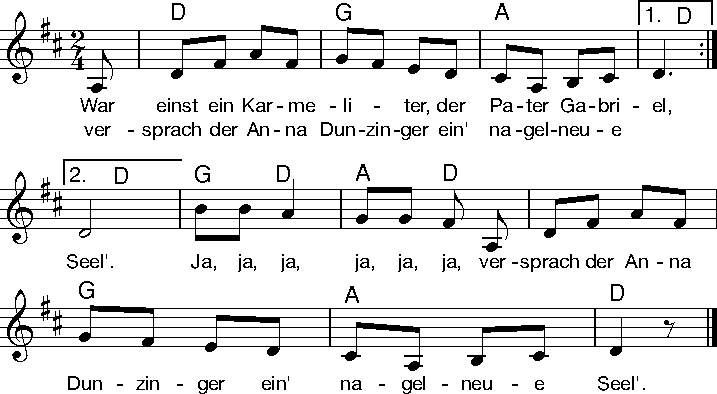
\includegraphics[width=1\textwidth]{Noten/Lied015.pdf}

\beginverse
\[D]Die Anna war ein \[G]Mädel und \[A]jung und wunder\[D]schön
und \[D]tat zum ersten \[G]Male ins \[A]Kloster beichten \[D]geh'n.
\[G]Ja-ja-\[D]ja, \[A]ja-ja-\[D]ja, und \[D]tat zum ersten \[G]Male ins \[A]Kloster beichten \[D]geh'n.
\endverse

\beginverse
^''Ei'', sprach er, ''liebes ^Annerl, komm ^doch zu mir he^rein!
Hier ^in dem dunk'len ^Kammerl kannst ^beichten ganz al^lein.''
^Ja-ja-^ja, ^ja-ja-^ja. ''Hier ^in dem dunk'len ^Kammerl kannst ^beichten ganz al^lein.''
\endverse

\beginverse
^Nahm sie in seinen ^Beichtstuhl, setzt ^sie auf seinen ^Schoß.
Da ^dacht' die Anna ^Dunzinger: Das ^Beichten geht fa^mos.
^Ja-ja-^ja, ^ja-ja-^ja, da ^dacht' die Anna ^Dunzinger: Das ^Beichten geht fa^mos.
\endverse

\beginverse
^Und er erzählt dem ^Annerl vom ^Berge Sina^i
Und ^greift ihr an die ^Waderln hi^nauf bis an die ^Knie.
^Ja-ja-^ja, ^ja-ja-^ja, und ^greift ihr an die ^Waderln hi^nauf bis an die ^Knie.
\endverse

\beginverse
^Nicht nur auf Haupt und ^Gliedern ruht ^die geweihte ^Hand,
Er ^senkt sie langsam ^nieder bis ^ins Gelobte ^Land.
^Ja-ja-^ja, ^ja-ja-^ja, er ^senkt sie langsam ^nieder bis ^ins Gelobte ^Land.
\endverse

\beginverse
^''Ei'', spricht er, ''liebes ^Annerl, greif ^in die Kutten, ^Maus,
Und ^hol mir meinen ^Priesterstab, ^den Segen Gottes, ^raus!''
^Ja-ja-^ja, ^ja-ja-^ja, ''Und ^hol mir meinen ^Priesterstab, ^den Segen Gottes, ^raus!''
\endverse

\beginverse
^Bald schwanden ihr die ^Sinne, wie ^leblos sank sie ^hin.
Da ^hat's nen kleinen ^Knacks gegeb'n, die ^neue Seel' war ^drin.
^Ja-ja-^ja, ^ja-ja-^ja, da ^hat's nen kleinen ^Knacks gegeb'n, die ^neue Seel' war ^drin.
\endverse

\beginverse
^D'rum all ihr kleinen ^Mädchen, wollt ^ihr 'ne neue ^Seel',
So ^geht zum Karme^liter, zum ^Pater Gabri^el.
^Ja-ja-^ja, ^ja-ja-^ja, so ^geht zum Karme^liter, zum ^Pater Gabri^el.
\endverse

\endsong

\beginscripture{}
Der Fall der Anna Dunzinger wurde 1872 von dem Wiener Julius Pederzani in seinem Werk "Die Opfer des Beichtstuhles" beschrieben. Bereits 1868 bezog ein Kapuzinerpater aus der Nähe von Aachen Stellung zu dem Sachverhalt des Liedes.
\endscripture

\begin{intersong}

\end{intersong}
\beginsong{Der kleine Troll}[wuw={mac (Erik Martin)}, bo={292}, pfii={10}, pfiii={40}, index={Steigt so ein kleiner Troll}]

\markboth{\songtitle}{\songtitle}

\beginverse 
\endverse

\centering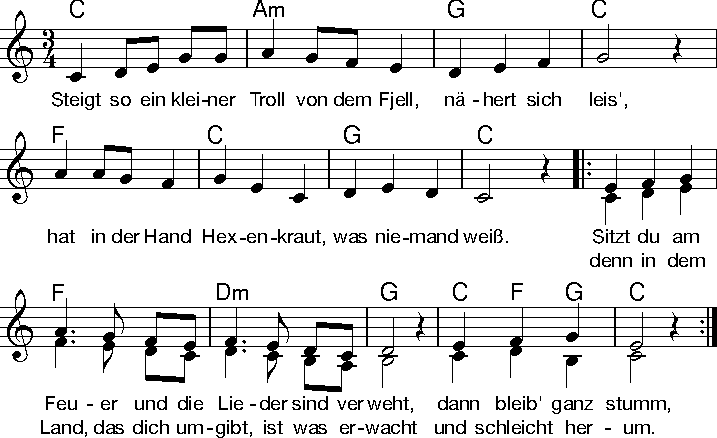
\includegraphics[width=1\textwidth]{Noten/Lied016.pdf}	

\beginverse
\[C]Plötzlich in deinem \[Am]Nacken spürst du \[G]eiskalten \[C]Hauch,
\[F]Atem des Trolls \[C]trifft dich wie \[G]giftiger \[C]Rauch.
\endverse 

\beginchorus
Sitzt du am \[F]Feuer und die \[Dm]Lieder sind ver\[G]weht, \[C]dann \[F]bleib \[G]ganz \[C]stumm,
denn in dem \[F]Land, das dich um\[Dm]gibt, ist was er\[G]wacht \[C]und \[F]schleicht \[G]he\[C]rum.
\endchorus 

\beginverse
^Du führst den Becher ^Tee nun zum Mund. ^Was zauderst ^du?
^Blütenstaub im ^Zaubertrank ^raubt dir die ^Ruh'.
\endverse
\renewcommand{\everychorus}{\textnote{\bf Refrain (wdh.) }}
\beginchorus
%Sitzt du am \[F]Feuer und die \[Dm]Lieder sind ver\[G]weht, \[C]dann \[F]bleib \[G]ganz \[C]stumm,
%denn in dem \[F]Land, das dich um\[Dm]gibt, ist was er\[G]wacht \[C]und \[F]schleicht \[G]he\[C]rum.
\endchorus

\beginverse
^Wenn du in dieser ^Nacht deinen Schlaf ^findest nicht ^mehr,
^der kleine Troll ^macht uns're ^Träume so ^schwer.
\endverse

\beginchorus
%Sitzt du am \[F]Feuer und die \[Dm]Lieder sind ver\[G]weht, \[C]dann \[F]bleib \[G]ganz \[C]stumm,
%denn in dem \[F]Land, das dich um\[Dm]gibt, ist was er\[G]wacht \[C]und \[F]schleicht \[G]he\[C]rum.
\endchorus


\endsong

\beginscripture{}
Der Autor (*1936), bekannt unter dem Fahrtennamen mac, verfasste viele bekannte Fahrtenlieder. Er beschäftigte sich intensiv mit skandinavischer Literatur und gab auch ein Jugendbuch mit dem Titel "Fjellwanderung" heraus.
\endscripture

\begin{intersong}

\end{intersong}
\beginsong{Der Mond ist aufgegangen}[txt={Matthias Claudius, 1778}, mel={Johann Abraham Peter Schulz, 1790}, pfiii={34}, index={Wie ist die Welt so stille}]

\markboth{\songtitle}{\songtitle}

\beginverse
\endverse 

\centering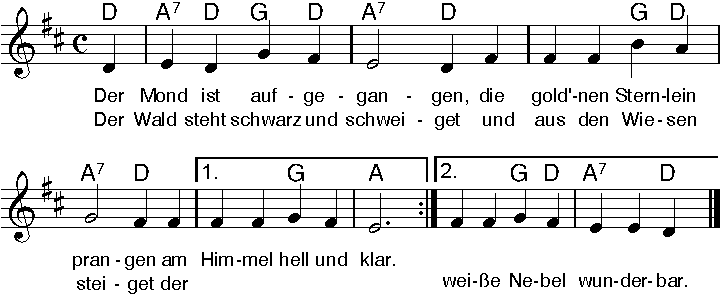
\includegraphics[width=1\textwidth]{Noten/Lied017.pdf}	

\beginverse
\[G]Wie \[D7]ist \[G]die \[C]Welt \[G]so \[D7]stil\[G]le und in der \[C]Dämm'\[G]rung \[D7]Höl\[G]le
so \[G]traulich \[C]und \[G]so \[D]hold! 
\[G]Als \[D7]ei\[G]ne \[C]stil\[G]le \[D7]Kam\[G]mer, wo ihr des \[C]Ta\[G]ges \[D7]Jam\[G]mer
ver\[G]schlafen \[C]und \[G]ver\[D7]gessen \[G]sollt.
\endverse

\beginverse
^Seht ^ihr ^den ^Mond ^dort ^ste^hen? Er ist nur ^halb ^zu ^se^hen
und ^ist doch ^rund ^und ^schön.
^So ^sind ^wohl ^man^che ^Sa^chen, die wir ge^trost ^be^lach^en,
weil ^uns're ^Au^gen ^sie nicht ^seh'n.
\endverse

\beginverse
^Wir ^stol^zen ^Men^schen^kin^der sind eitel ^ar^me ^Sün^der
und ^wissen ^gar ^nicht ^viel.
^Wir ^spin^nen ^Luft^ge^spin^ste und suchen ^vie^le ^Kün^ste
und ^kommen ^wei^ter ^von dem ^Ziel.
\endverse

\beginverse
^Gott, ^lass ^dein ^Heil ^uns ^schau^en, auf nichts Ver^gang^lich's ^trau^en,
nicht ^Eitel^keit ^uns ^freu'n!
^Lass ^uns ^ein^fal^tig ^wer^den, und vor dir ^hier ^auf ^Er^den
wie ^Kinder ^fromm ^und ^fröhlich ^sein!
\endverse

\beginverse
^Wollst ^end^lich ^son^der ^Grä^men aus dieser ^Welt ^uns ^neh^men
durch ^einen ^sanf^ten ^Tod.
^Und ^wenn ^du ^uns ^ge^nom^men, lass uns in ^Him^mel ^kom^men,
du ^unser ^Herr ^und ^unser ^Gott!
\endverse

\beginverse
^So ^legt ^euch ^denn, ^ihr ^Brüder, in Gottes ^Na^men ^nie^der,
kalt ^ist der ^A^bend^hauch.
^Ver^schon' ^uns, ^Gott, ^mit ^Stra^fen und lass uns ^ru^hig ^schla^fen
und ^unser'n ^kran^ken ^Nachbar ^auch!
\endverse

\endsong

\beginscripture{}
Dem Gedicht von Claudius als Vorlage diente "Nun ruhen alle Wälder" (1653) von Paul Gerhardt. Caulius' Todesgedicht vor dem Hintergrund der Heilserwartung eines Christen könnte auch schon vor 1778 in Darmstadt entstanden sein. Seine Einfachheit wurde teilweise als naiv kritisiert, erfreute sich jedoch schnell großer Beliebtheit in der deutschen Bevölkerung.
\endscripture

\begin{intersong}

\end{intersong}
\beginsong{Der Pfahl}[wuw={Luis Lach, übersetzt von Oss Kröher, 1968}, pfiii={56}, index={Sonnig begann es zu tagen}]

\markboth{\songtitle}{\songtitle}

\beginverse
\endverse

\centering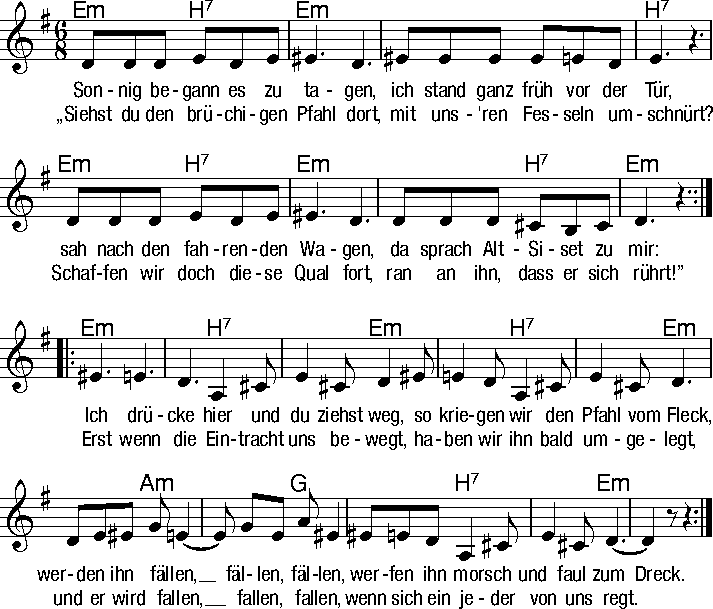
\includegraphics[width=1\textwidth]{Noten/Lied018.pdf}	

\beginverse
\[Em]'Ach Siset, \[H7]noch ist es \[Em]nicht geschafft, an meiner Hand platzt die \[H7]Haut.
\[Em]Langsam auch \[H7]schwindet schon \[Em]meine Kraft, er ist zu \[H7]mächtig ge\[Em]baut.
Wird es uns \[H7]jemals ge\[Em]lingen? Siset, es fällt mir so \[H7]schwer!'
\[Em]'Wenn wir das \[H7]Lied nochmal \[Em]singen, geht es viel \[H7]besser. Komm \[Em]her!'
\endverse

\beginchorus 
\[Em]Ich drücke \[H7]hier und du ziehst \[Em]weg, so kriegen \[H7]wir den Pfahl vom \[Em]Fleck,
werden ihn \[Am]fällen, fällen, \[G]fällen, werfen ihn \[H7]morsch und faul zum \[Em]Dreck.
Erst wenn die \[H7]Eintracht uns be\[Em]wegt, haben wir \[H7]ihn bald umge\[Em]legt
und er wird \[Am]fallen, fallen, \[G]fallen, wenn sich ein \[H7]jeder von uns \[Em]regt!
\endchorus

\beginverse
^Der alte ^Siset sagt ^nichts mehr, böser Wind hat ihn ver^weht.
^Keiner weiß ^von seiner ^Heimkehr, keiner weiß, ^wie es ihm ^geht.
Alt-Siset ^sagte uns ^allen, hör es auch du, krieg es ^mit:
^Der morsche ^Pfahl wird schon ^fallen, wie es ge^schieht in dem ^Lied.
\endverse
\renewcommand{\everychorus}{\textnote{\bf Refrain (wdh.)}}
\beginchorus
\endchorus

\endsong

\beginscripture{}
Das Lied ist die Übersetzung von L'estaca von Luis Lach. Der Pfahl ist hier Sinnbild für den Staat. Das Lied ist zur Zeit der Diktatur in Katalonien bekannt geworden.
\endscripture

\begin{intersong}

\end{intersong}
\beginsong{Der Piet am Galgen hängt}[wuw={Erik Martin, 1981}, bo={364}, pfii={69}, pfiii={25}, index={Was kann ich denn dafür}]

\markboth{\songtitle}{\songtitle}

\beginverse 
\endverse

\centering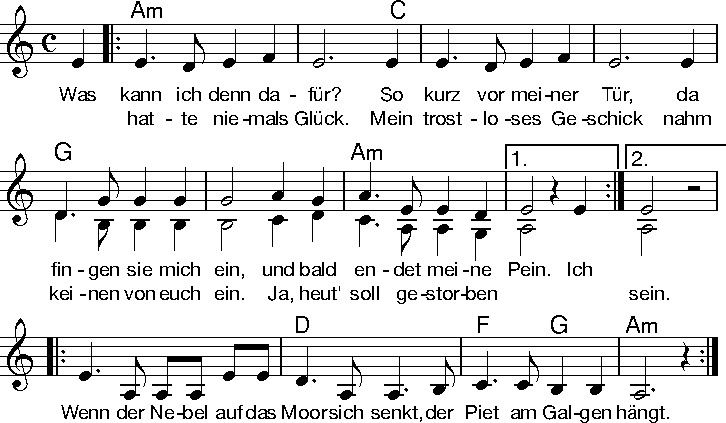
\includegraphics[width=1\textwidth]{Noten/Lied019.pdf}	

\beginverse
Sie \[Am]nahmen mir die Schuh' und \[C]auch den Rock dazu.
Sie \[G]banden mir die Händ' und mein \[Am]Haus, es hat gebrennt. 
Ich \[Am]sah den Galgen steh'n. Sie \[C]zwangen mich zu geh'n. 
Sie \[G]wollten meinen Tod, keiner \[Am]half mir in der Not.
\endverse

\beginchorus
\lrep \[Am]Wenn der Nebel auf das \[D]Moor sich senkt, der \[F]Piet am \[G]Galgen \[Am]hängt.\rrep
\endchorus

\beginverse
Was ^kratzt da am Genick? Ich ^spür' den rauhen Strick.
Ein ^Mönch der betet dort und spricht ^für mich fromme Wort,
die Wort, die ich nicht kenn', wer ^lehrte sie mich denn? 
Fünf ^Raben fliegen her, doch ich ^sehe sie nicht mehr.
\endverse
%\renewcommand{\everychorus}{\textnote{\bf Refrain (wdh.) }}
\beginchorus
\lrep \[Am]Wenn der Nebel auf das \[D]Moor sich senkt, der \[F]Piet am \[G]Galgen \[Am]hängt.\rrep
\endchorus

\endsong

\beginscripture{}
Der Verfasser lässt im Unklaren, auf wen sich die Person des Piet tatsächlich bezieht. Es sind jedoch Parallelen zum Schinderhannes erkennbar.
\endscripture

\begin{intersong}
\ifthenelse{\boolean{pics}}{
\vspace{25pt}
\centering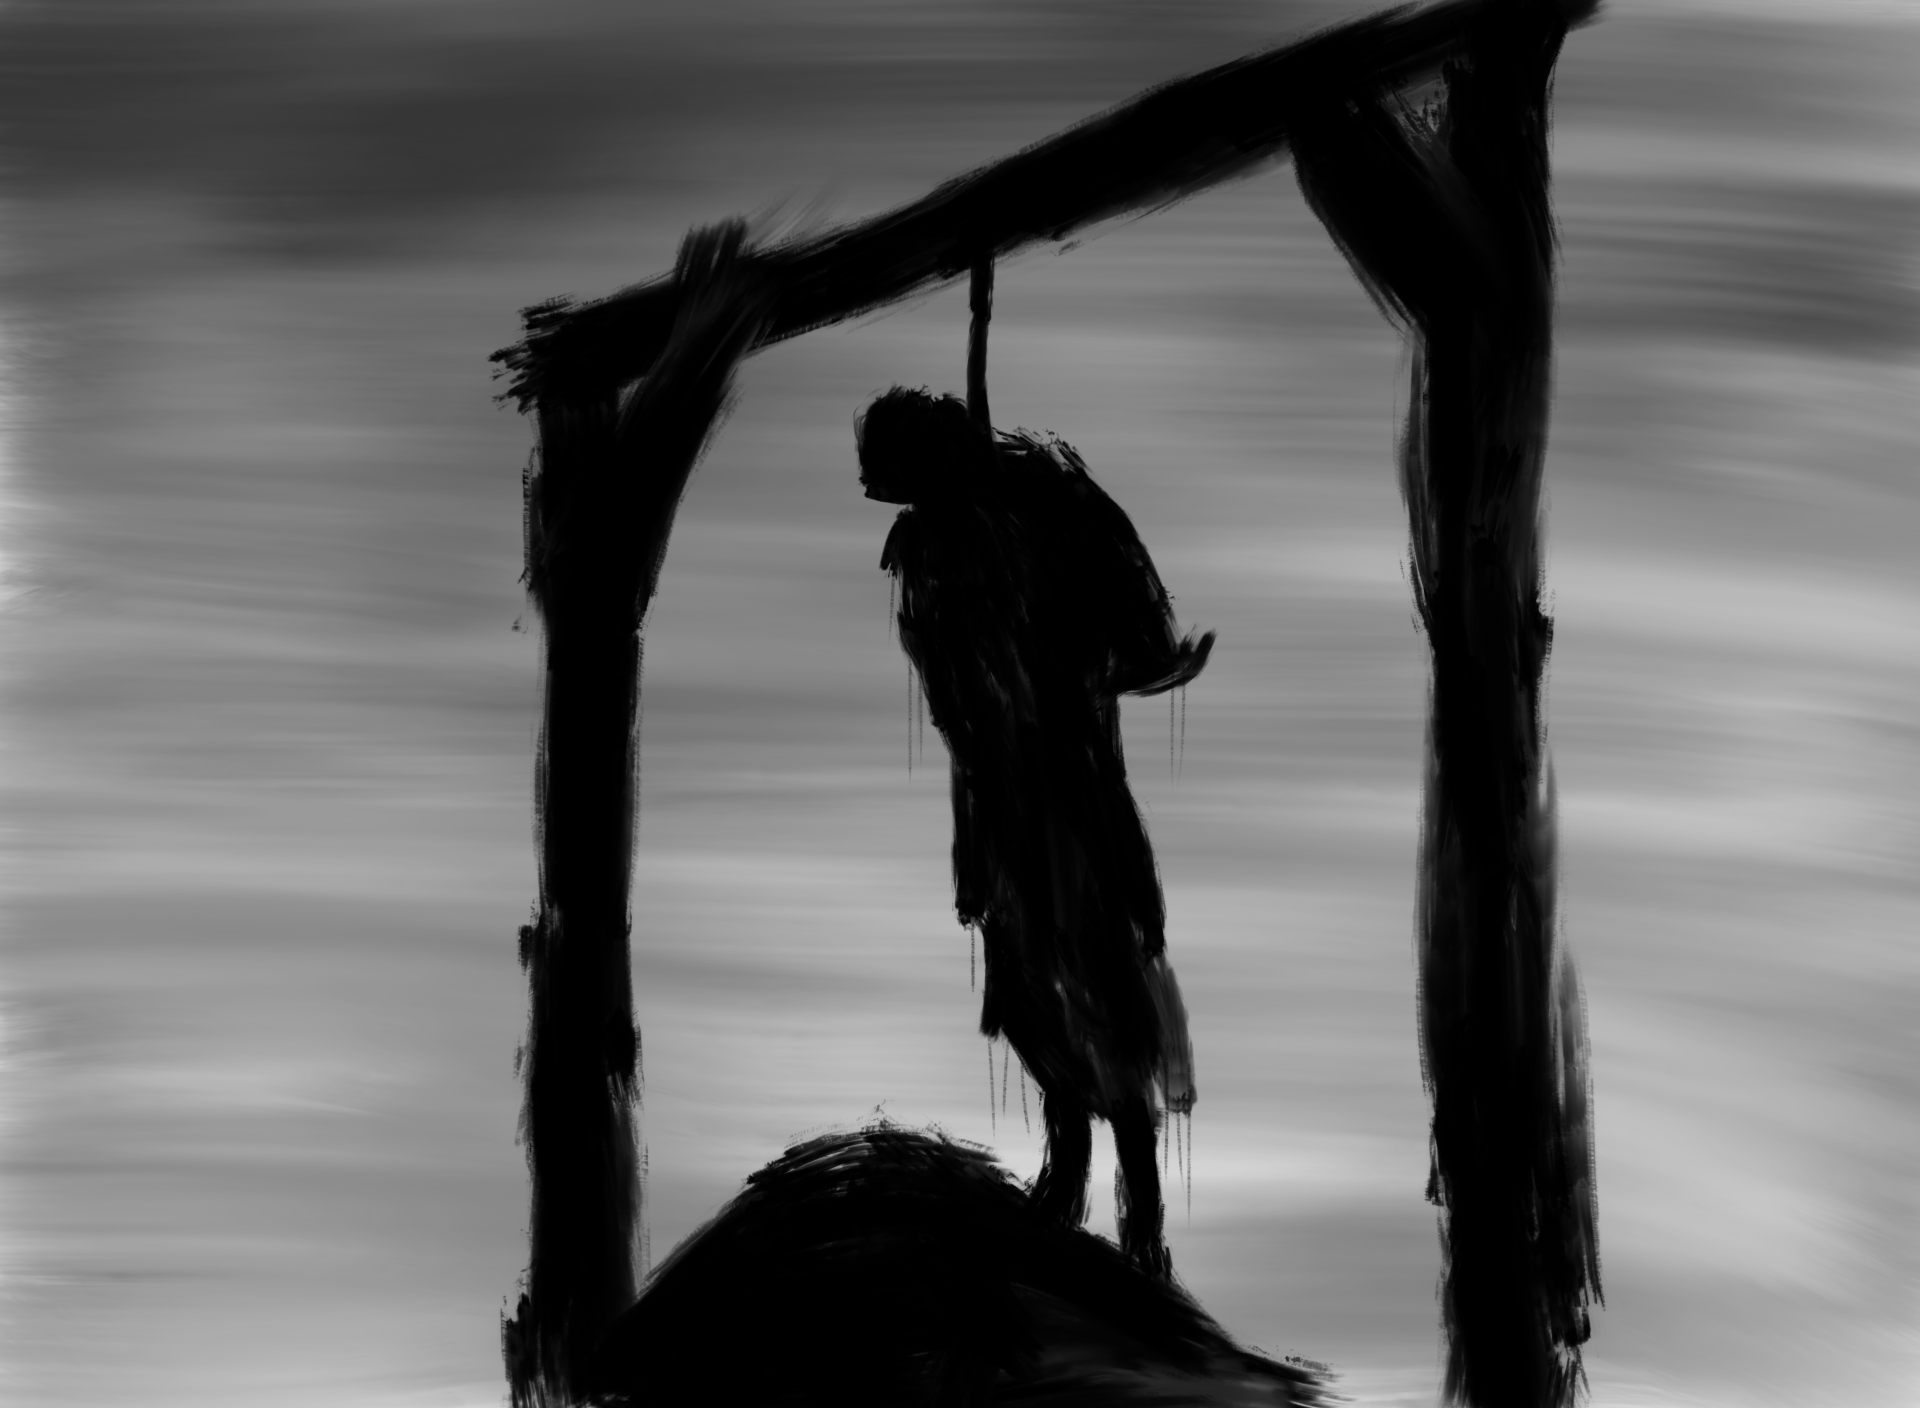
\includegraphics[width=1\textwidth]{Bilder/piet_heiko.png}	
}{}
\end{intersong}
\beginsong{Der Tod und der Mediziner}[mel={August Harder, ca. 1810}, txt={Gotthold Ephraim Lessing, 1747}, bo={168}, pfii={124}, pfiii={38}, index={Gestern Brüder könnt ihr‘s glauben, Tod und Mediziner}]

\markboth{\songtitle}{\songtitle}

\beginverse 
\endverse

\centering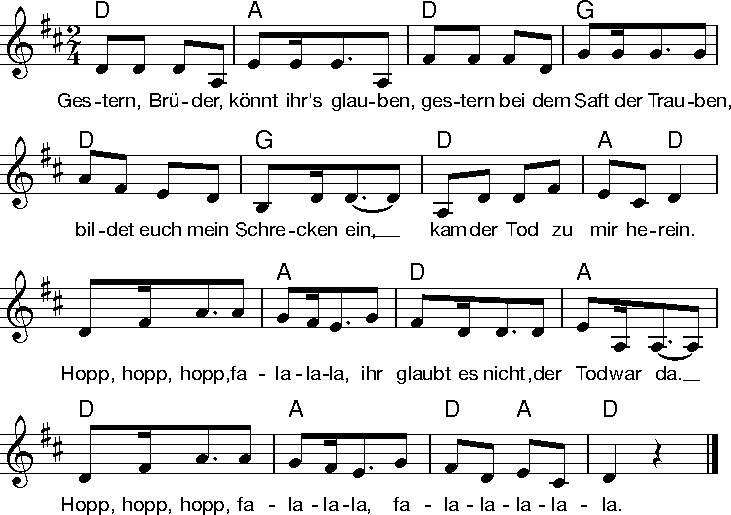
\includegraphics[width=1\textwidth]{Noten/Lied020.pdf}	

\beginverse\memorize
\[D]Drohend schwang er \[A]seine Hippe, \[D]drohend sprach das \[G]Furchtgerippe:
\[D]''Fort, du treuer \[G]Bacchusknecht! \[D]Fort, du hast ge\[A]nug ge\[D]zecht!''
\[D]''Lieber Tod'', sprach \[A]ich mit Tränen, \[D]''solltest du dich \[G]nach mir sehnen,
\[D]siehe, da steht \[G]Wein für dich. \[D]Lieber Tod, ver\[A]schone \[D]mich!''
\endverse

\beginchorus
\[D]Hopp, hopp, hopp, fa-\[A]la-la-la, ihr \[D]glaubt es nicht: Der \[A]Tod war da.
\[D]Hopp, hopp, hopp, fa-\[A]la-la-la, fa-\[D]la-la-\[A]la-la-\[D]la.
\endchorus


\beginverse
^Lächelnd greift er ^nach dem Glase, ^lächelnd trinkt er's ^aus der Base
^Auf der Pest Ge^sundheit leer, ^lächelnd stellt er's ^wieder ^her.
^Fröhlich glaubt' ich ^mich befreit, ^als er schnell sein ^Droh'n erneuert:
^''Narre, für ein ^Gläschen Wein ^denkst du'', sprach er, ^''los zu ^sein?''
\endverse
\renewcommand{\everychorus}{\textnote{\bf Refrain (wdh.)}}
\beginchorus
\endchorus

\beginverse
^''Tod'', sprach ich, ''ich ^möcht' auf Erden ^gern ein Medi^ziner werden.
^Lass mich, ich ver^spreche dir ^meine Kranken ^halb da^für!''
^''Gut, wenn das ist, ^magst du leben'', ^ruft er. ''Nun sei ^mir ergeben!
^Lebe, bis du ^sattgeküsst ^und des Trinkens ^müde ^bist!''
\endverse

\beginchorus
\endchorus

\beginverse
^Oh, wie schön klingt ^das den Ohren? ^''Tod, du hast mich ^neu geboren!
^Dieses Glas voll ^Rebensaft, ^Tod, auf gute ^Brüder^schaft!''
^Ewig muss ich ^also leben, ^ewig denn dein ^Gott der Reben,
^ewig soll mich ^Lieb' und Wein, ^ewig Wein und ^Lieb' er^freu'n.
\endverse

\beginchorus
\endchorus

\endsong

\beginscripture{}
%nix g'fund'n
\endscripture

\begin{intersong}
\ifthenelse{\boolean{pics}}{
\ThisLRCornerWallPaper{0.35}{Bilder/TodUndMediziner_heiko.png}
}{}
\end{intersong} %BILD, Alter!
\beginsong{Die Brombeeren}[wuw={Volkslied aus Lothringen, 19. Jahrhundert}, bo={144}, pfii={78}, pfiii={41}, index={Es wollt ein Mägdlein}]

\markboth{\songtitle}{\songtitle} 

\beginverse
\endverse

\centering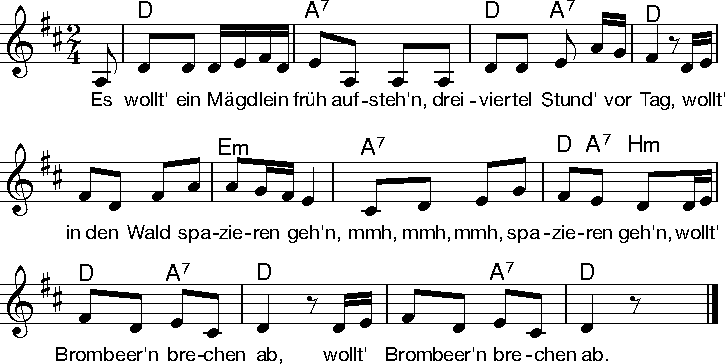
\includegraphics[width=1\textwidth]{Noten/Lied021.pdf}	

\beginverse
Und \[D]als sie in den \[A7]Wald 'nein kam, da \[D]kam des \[A7]Jägers K\[D]necht:
''Ei Mädchen, scher dich \[Em]aus dem Wald! \[A7]Mmmh mmmh \[D]aus \[A7]dem \[Hm]Wald!
\lrep  Meinem \[D]Herr'n, dem \[A7]ist's nicht \[D]recht.'' \rrep
\endverse

\beginverse
Und ^als sie ein Stück ^weiter kam, da ^kam des ^Jägers ^Sohn:
''Ei Mädchen, setz dich ^nieder, ^mmmh mmmh setz dich ^ni^e^der,
\lrep  zupf ^dir dein ^Körblein ^voll!'' \rrep
\endverse

\beginverse
''Ein ^Körblein voll, das b^rauch ich nicht, ein ^Handvoll ^ist ge^nug.
In meines Vaters ^Garten, ^mmmh mmmh ^Ga^r^ten,
\lrep  da ^wachsen ^Brombeeren ^genug.' \rrep
\endverse

\beginverse
So ^schön wie braune ^Bären sah ^sie seine ^Äuglein ^steh'n.
Wer kann im grünen ^Walde, ^mmmh mmmh im grünen ^Wa^l^de,
\lrep den ^Beeren ^wider^steh'n? \rrep
\endverse

\beginverse
Und ^als dreiviertel Jahr ver^gangen war'n, die ^Brombeeren ^wurden ^groß,
da hat das schwarzbraun ^Mägdelein, ^mmmh mmmh das ^Mäg^de^lein,
\lrep ein ^Kind auf ^ihrem ^Schoß. \rrep
\endverse

\beginverse
Sie ^schaut es mit Ver^wund'rung an: 'Ei ^ei, was ^hab' ich denn ge^tan?
Kommt das wohl von den ^Brombeeren, ^mmmh mmmh, von den ^Brom^bee^ren,
\lrep die ^ich ge^pflücket ^hab'?' \rrep
\endverse

\beginverse
D'rum ^wer ein ehrliches ^Mägdlein will ham, der ^schick sie nicht ^in den ^Wald,
denn im Wald da wachsen ^Brombeeren, ^ja, ja, ja, die ^Brom^bee^ren,
\lrep und die ^reifen manchmal ^viel zu ^bald. \rrep
\endverse


\endsong

\beginscripture{}
% nix g'fund'n
\endscripture

\begin{intersong}

\end{intersong}
\beginsong{Die freie Republik}[wuw={Studentengruppen, Januar 1937}, bo={206}, pfii={47}, pfiii={23}, index={In dem Kerker saßen}]

\markboth{\songtitle}{\songtitle} 

\beginverse
\endverse

\centering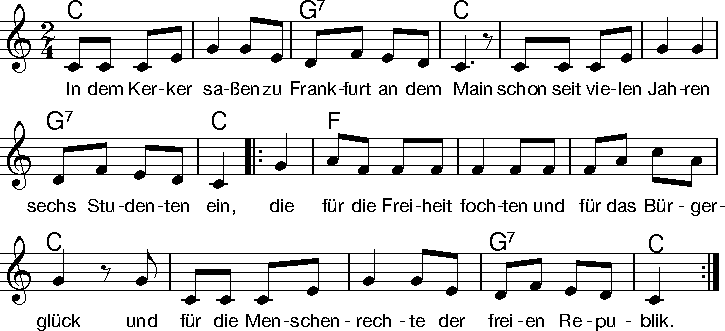
\includegraphics[width=1\textwidth]{Noten/Lied022.pdf}	

\beginverse
\[C]Und der Kerkermeister \[G7]sprach es täglich \[C]aus:
''Sie, Herr Bürgermeister, es \[G7]reißt mir keiner \[C]aus!''
\lrep Aber \[F]doch sind sie verschwunden abends aus dem \[C]Turm,
um die zwölfte Stunde, \[G7]bei dem großen \[C]Sturm. \rrep
\endverse

\beginverse
^Und am ander'n Morgen ^hört man den A^larm.
Oh, es war entsetzlich, ^der Soldaten^schwarm!
\lrep Sie ^suchten auf und nieder, sie suchten hin und ^her,
sie suchten sechs Studenten und ^fanden sie nicht ^mehr. \rrep
\endverse

\beginverse
^Doch sie kamen wieder, mit ^Schwertern in der ^Hand.
''Auf, auf, ihr deutschen Brüder, jetzt ^geht's für's Vater^land!
\lrep Jetzt ^geht's für Menschenrechte und für das Bürger^glück!
Wir sind doch keine Knechte der ^freien Repu^blik.'' \rrep
\endverse

\beginverse
^Wenn euch die Leute fragen: ''^Wo ist Absa^lom?''
So dürfet ihr wohl sagen: ''^Oh, der hänget ^schon.''
\lrep Er ^hängt an keinem Baume, er hängt an keinem ^Strick,
sondern an dem Glauben an die ^freie Repu^blik. \rrep
\endverse


\endsong

\beginscripture{}
Erkennungslied der demokratischen Bewegung zu jener Zeit. Text und Musik entstanden nach der Befreiung von 6 Studenten, die mit dem Frankfurter Wachensturm (auf die Hauptwache und die Konstablerwache) vom 3. April 1833 versucht hatten, eine Revolution auszulösen. Ihre Flucht gelang schließlich mit Hilfe der Gefangenenwärter. In Folge dieser Verschwörung wurden mehr als 1.800 Personen zur Fahndung ausgeschrieben und 39 Personen zum Tod oder zu lebenslanger Haft verurteilt.
\endscripture

\begin{intersong}

\end{intersong}
\beginsong{Die Gedanken sind frei}[txt={Hoffmann von Fallersleben nach einem Flugblatt, 1780}, mel={ca. 1810 - 1820}, pfii={115}, pfiii={31}]

\markboth{\songtitle}{\songtitle} 

\beginverse
\endverse

\centering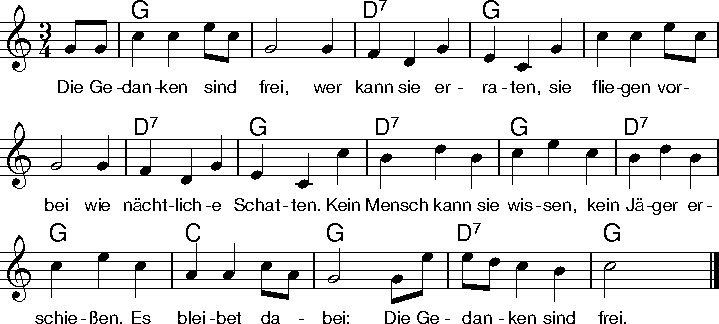
\includegraphics[width=1\textwidth]{Noten/Lied023.pdf}

\beginverse
Ich \[G]denke, was ich will und \[D7]was mich be\[G]glücket, 
und alles in der Still', und \[D7]wie es sich \[G]schicket.
Mein \[D7]Wunsch und Be\[G]gehren kann \[D7]niemand ver\[G]wehren.
Es \[C]bleibet da\[G]bei: Die Ge\[D7]danken sind \[G]frei!
\endverse 

\beginverse
Und ^sperrt man mich ein im ^finsteren ^Kerker,
das alles sind rein ver^gebliche ^Werke,
denn ^meine Ge^danken zer^reißen die ^Schranken
und ^Mauern ent^zwei: Die Ge^danken sind ^frei!
\endverse

\beginverse
Nun ^will ich auf immer den ^Sorgen ent^sagen
und will mich auch nimmer mit ^Grillen mehr ^plagen.
Man ^kann ja im ^Herzen stets ^lachen und ^scherzen
und ^denken da^bei: Die Ge^danken sind ^frei!
\endverse

\beginverse
Ich ^liebe den Wein, mein ^Mädchen vor ^allen,
die tut mir allein am ^Besten ge^fallen.
Ich ^bin nicht al^leine bei ^einem Glas ^Weine;
mein ^Mädchen da^bei: Die Ge^danken sind ^frei!
\endverse

\endsong

\beginscripture{}
Das Lied wurde zuerst in der Sammlung „Lieder der Brienzer Mädchen“ in Bern gedruckt. Im Jahr 1842 wurde das Lied in „Schlesische Volkslieder“ von Hoffmann von Fallersleben und Ernst Richter veröffentlicht. Diese letzte Version stammt von Hoffmann von Fallersleben. Es diente in Zeiten politischer Unterdrückung immer wieder zum Ausdruck der Sehnsucht nach Freiheit und Unabhängigkeit, so zum Beispiel in der Studentenbewegung im 19. Jahrhundert, im Dritten Reich oder während der Berlin-Blockade 1948. 
\endscripture



%\end{intersong}
\beginsong{Die Internationale}[wuw={Eugène Pottier, Pierre Degeyter, 1871}, index={Wacht auf, Verdammte dieser Erde}]

\markboth{\songtitle}{\songtitle}

\beginverse
\endverse

\centering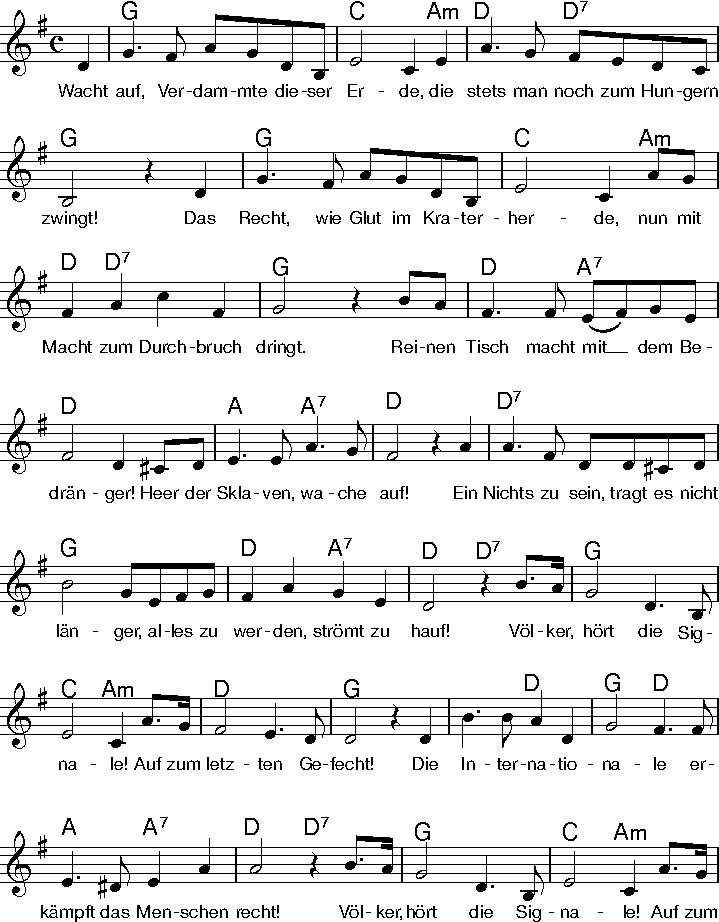
\includegraphics[width=1\textwidth]{Noten/Lied023a.pdf} 	

\beginverse*
\endverse

\centering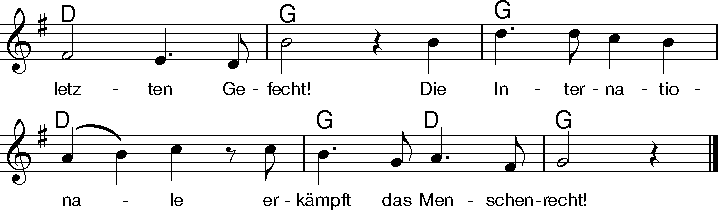
\includegraphics[width=1\textwidth]{Noten/Lied023a_1.pdf}	

\beginverse
Es \[G]rettet uns kein höh'res \[C]Wesen, kein \[D]Gott, kein \[D7]Kaiser noch Tri\[G]bun.
Uns \[G]aus dem Elend zu er\[C]lösen, können \[D]wir nur \[D7]selber \[G]tun.
\[D]Leeres Wort: Des \[A7]Armen \[D]Rechte! Leeres \[A]Wort: Des \[A7]Reichen \[D]Pflicht!
Un\[D7]mündig nennt man uns \[G]Knechte! Duldet die \[D]Schmach nun \[A7]länger \[D]nicht!\[D7]
\endverse

\beginchorus

Völker, \[G]hört die Sig\[C]nale, auf zum \[D]letzten Ge\[G]fecht!
Die Inter\[D]natio\[G]na\[D]le er\[A]kämpft das \[A7]Menschen\[D]recht\[D7]!
Völker, \[G]hört die Sig\[C]nale, auf zum \[D]letzten Ge\[G]fecht!
Die \[G]Internatio\[D]nale er\[G]kämpft das \[D]Menschen\[G]recht!
\endchorus

\beginverse
In ^Stadt und Land, ihr Arbeits^leute, sind ^wir die ^stärkste der Par^tei'n.
Die ^Müßiggänger schiebt bei^seite! Diese ^Welt muss ^unser ^sein!
Unser ^Blut ^sei nicht mehr der ^Raben und der ^mächt'gen ^Geier ^Fraß!
Erst ^wenn wir sie vertrieben ^haben, dann scheint die ^Sonn' ohn' ^Unter^lass^!
\endverse
\renewcommand{\everychorus}{\textnote{\bf Refrain (wdh.)}}
\beginchorus
\endchorus

\endsong

\beginscripture{}
Die Internationale ist das weltweit am weitesten verbreitete Kampflied der sozialistischen Arbeiterbewegung. Sie entstand im Zuge der Pariser Kommune von März bis Mai 1871, der ersten als proletarisch-sozialistisch geltenden Revolution.
\endscripture

\begin{intersong}

\end{intersong}
\beginsong{Die Lappen hoch}[wuw={Jurij Andreev, Nerother Wandervogel, 1954}, bo={78}, pfii={38}, pfiii={17}]

\markboth{\songtitle}{\songtitle}

\beginverse
\endverse

\centering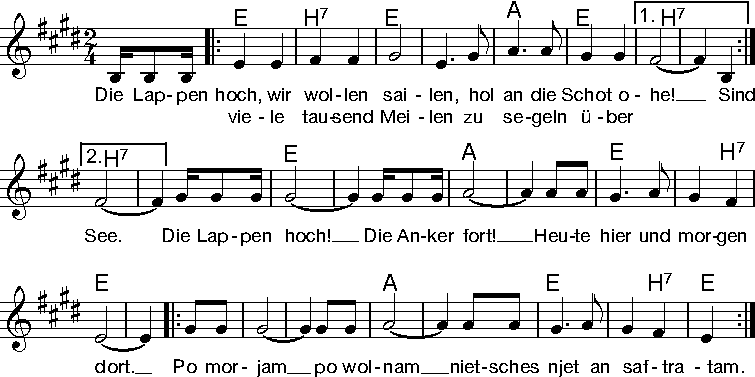
\includegraphics[width=1\textwidth]{Noten/Lied024.pdf}	

\beginverse
Wenn einst \[E]am La\[H7]gunen\[E]rande in \[A]Lee liegt \[E]unser \[H7]Boot,
Lacht \[E]uns das \[H7]Glück am \[E]Strande, am \[A]Strande \[E]gelb und \[H7]rot.
\endverse

\beginchorus
Die Lappen \[E]hoch, die Anker \[A]fort, heute \[E]hier und \[H7]morgen \[E]dort.
Po morjam, po wol\[A]nam nietsches \[E]njet an \[H7]Safra\[E]tam.
\endchorus

\beginverse
Und nie ^würdest ^weiter du ^ziehen und ^ewig ^bliebest du ^dann,
Ja, ^wenn nicht ^wäre das ^Segeln, ^der Wind und der ^Oze^an.
\endverse
\renewcommand{\everychorus}{\textnote{\bf Refrain (wdh.)}}
\beginchorus
\endchorus

\endsong

\beginscripture{}
''Po morjam...'' bedeutet: Auf's Meer, auf die Wellen, heute hier und morgen dort!
\endscripture

\begin{intersong}

\end{intersong}
\beginsong{Die Regenfrau}[wuw={tejo (Walter Scherf), 1953}, bo={60}, index={Der Nebel dämpft das Morgenlicht}]

\markboth{\songtitle}{\songtitle}

\beginverse
\endverse

\centering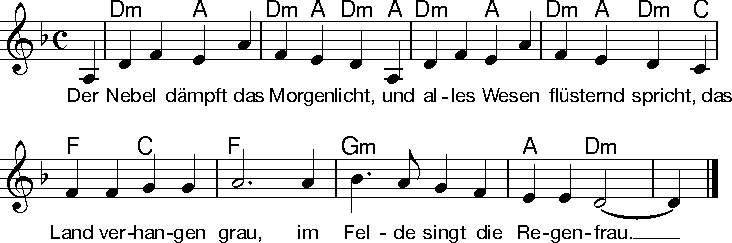
\includegraphics[width=1\textwidth]{Noten/Lied026.pdf}	

\beginverse
Der \[Dm]Weg ist \[A]lang, der \[Dm]Weg \[A]ist \[Dm]weit, \[A]wir \[Dm]wandern \[A]tief am \[Dm]Grund \[A]der \[Dm]Zeit.
Der \[F]Sommer \[C]ist ver\[F]brannt, ein \[Gm]fahler Rauch weht \[A]durch das \[Dm]Land.
\endverse

\beginverse
Das ^Jahr geht ^aus, der ^Re^gen ^fällt, ^ein ^and'rer ^Herr re^giert ^die ^Welt.
Der ^Wind ist ^nass und ^schwer, das ^Land ertrinkt im ^Regen^meer.
\endverse

\endsong

\beginscripture{}
tejo arbeitete auch als Übersetzer, das bekannteste von ihm übersetzte Werk ist ''Der kleine Hobbit'' von J. R. R. Tolkien.
\endscripture

\begin{intersong}
\end{intersong} % 025, 026 getauscht -> platz
\beginsong{Die Moorsoldaten}[mel={Rudi Goguel, Hans Eigler, 1933}, txt={Johann Esser, Wolfgang Langhoff, 1933}, bo={420}, pfii={68}, pfiii={42}, index={Wohin auch das Auge blicket}]

\markboth{\songtitle}{\songtitle}

\beginverse
\endverse

\centering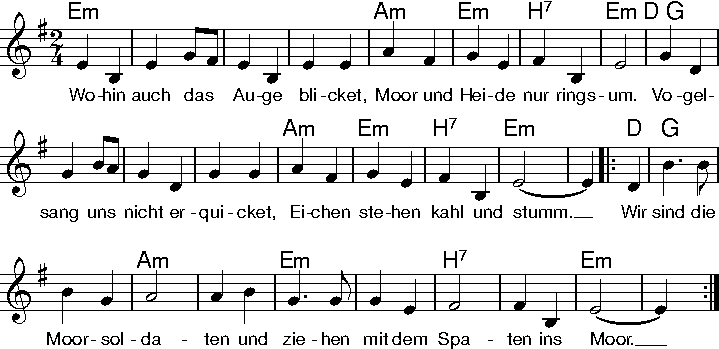
\includegraphics[width=1\textwidth]{Noten/Lied025.pdf}	

\beginverse
\[Em]Hier in dieser öden Heide \[Am]ist das \[Em]Lager \[H7]aufge\[Em]baut, \[D]
\[G]wo wir fern von jeder Freude \[Am]hinter \[Em]Stachel\[H7]draht ver\[Em]staut.
\endverse

\beginchorus
\lrep \[D]Wir \[G]sind die Moorsol\[Am]daten und \[Em]ziehen mit dem \[H7]Spaten ins \[Em]Moor! \rrep
\endchorus

\beginverse
^Morgens ziehen die Kolonnen ^in das ^Moor zur ^Arbeit ^hin, ^
^Graben bei dem Brand der Sonne, ^doch zur ^Heimat ^steht der ^Sinn.
\endverse
%\renewcommand{\everychorus}{\textnote{\bf Refrain (wdh.)}}
\beginchorus
\lrep \[D]Wir \[G]sind die Moorsol\[Am]daten und \[Em]ziehen mit dem \[H7]Spaten ins \[Em]Moor! \rrep
\endchorus
\beginverse
^Heimwärts, heimwärts! Jeder sehnet ^sich nach ^Eltern, ^Weib und ^Kind. ^
^Manche Brust ein Seufzer dehnet, ^weil wir ^hier ge^fangen ^sind.
\endverse

\beginchorus
\lrep \[D]Wir \[G]sind die Moorsol\[Am]daten und \[Em]ziehen mit dem \[H7]Spaten ins \[Em]Moor! \rrep
\endchorus

\beginverse
^Auf und nieder geh'n die Posten; ^keiner, ^keiner ^kann hin^durch. ^
^Flucht wird nur das Leben kosten, ^vierfach ^ist um^zäunt die ^Burg.
\endverse

\beginchorus
\lrep \[D]Wir \[G]sind die Moorsol\[Am]daten und \[Em]ziehen mit dem \[H7]Spaten ins \[Em]Moor! \rrep
\endchorus

\beginverse
^Doch für uns gibt es kein Klagen, ^ewig ^kann's nicht ^Winter ^sein. ^
^Einmal werden froh wir sagen: ''^Heimat, ^Du bist ^wieder ^mein!''
\endverse

%\renewcommand{\everychorus}{\textnote{\bf Refrain}}
\beginchorus
\lrep \[D]Dann \[G]zieh'n die Moorsol\[Am]daten \[Em]nicht mehr mit dem \[H7]Spaten in's \[Em]Moor! \rrep
\endchorus

\endsong

\beginscripture{}
Das Lied entstand 1933 im Konzentrationslager Börgermoor (im Emsland), in dem hauptsächlich politische Gefangene untergebracht waren. Obwohl die Lagerleitung es schnell verbot, beförderte das Wachpersonal den Gesang des Liedes. Es wurde auch in anderen Moorlagern gesungen und von entlassenen Häftlingen verbreitet, sodass es sogar der Moskauer Rundfunk zu Ehren deutscher Antifaschisten spielte.
\endscripture

\begin{intersong}
\end{intersong}
\beginsong{Die schlesischen Weber}[txt={Heinrich Heine, 1844}, mel={helm (Helmut König)}, bo={196}, pfii={50}, pfiii={24}, index={Im düsteren Auge}]

\markboth{\songtitle}{\songtitle}


\beginverse*
{\nolyrics Intro: \[Em] \[C] \[D] \rep{2}}\newline
\endverse

\beginverse
\endverse
\centering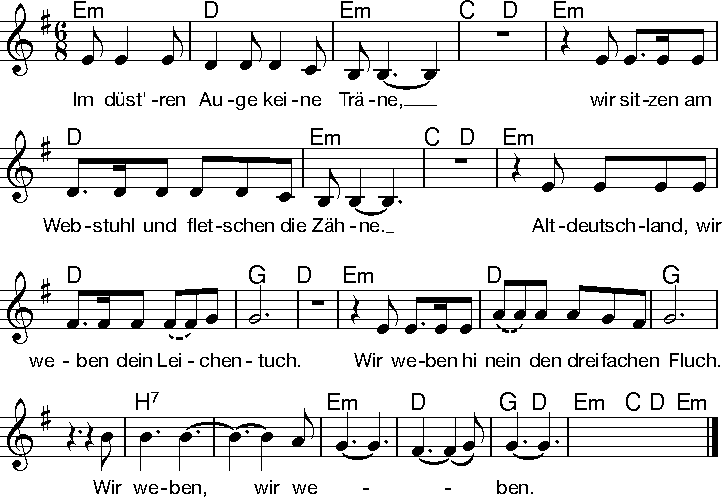
\includegraphics[width=1\textwidth]{Noten/Lied027.pdf}	

\beginverse\memorize
\[Em]Ein Fluch dem \[D]Gotte zu dem wir ge\[Em]beten \[C] \[D] \[Em]
in Winters\[D]kälte und Hungers\[Em]nöten. \[C] \[D] \[Em]
Wir haben ver\[D]gebens gehofft und ge\[G]harrt. \[D]
\[Em]Man hat uns ge\[D]äfft, gefoppt und ge\[G]narrt.
\endverse

\beginchorus
Wir \[H7]weben, wir \[Em]we \[D]- \[G]ben. \[D] \[Em] \[C] \[D] \[Em] \[C] \[D]
\endchorus

\beginverse
^Ein Fluch dem ^König, dem König der ^Reichen, ^ ^ ^
den unser ^Elend nicht konnte er^weichen, ^ ^ ^
der den letzten ^Groschen von uns er^presst ^
^und uns wie ^Hunde erschießen ^lässt.
\endverse

\renewcommand{\everychorus}{\textnote{\bf Refrain (wdh.)}}
\beginchorus
\endchorus

\beginverse
^Ein Fluch dem ^falschen Vater^lande, ^ ^ ^
wo nur ge^deihen Schmach und ^Schande, ^ ^ ^
wo jede ^Blume früh ge^knickt, ^
^wo Fäulnis und ^Moder den Wurm er^quickt.
\endverse

\beginchorus
\endchorus

\beginverse
^Das Schifflein ^fliegt, der Webstuhl ^kracht. ^ ^ ^
Wir weben ^emsig Tag und ^Nacht. ^ ^ ^
Altdeutschland wir ^weben dein Leichen^tuch, ^
^wir weben hi^nein den dreifachen ^Fluch.
\endverse

\beginchorus
\endchorus


\endsong

\beginscripture{}
Das Lied beschreibt das Elend der schlesischen Weber, die 1844 im Zuge der Industrialisierung zum Protest gegen Ausbeutung und Lohnverfall einen Aufstand organisierten. Es wurde zuerst in Karl Marx' Flugschrift ''Vorwärts!'' veröffentlicht. Das Königlich Preußische Kammergericht verbot das Gedicht und seine Rezitation bei Gefängnisstrafe.
\endscripture

\begin{intersong}

\end{intersong}
\beginsong{Donna, donna}[wuw={Shalom Secunda, Aaron Zeitlin, 1940}, pfii={220}, pfiii={50}, index={On a wagon bound for market}]

\markboth{\songtitle}{\songtitle}

\beginverse
\endverse

\centering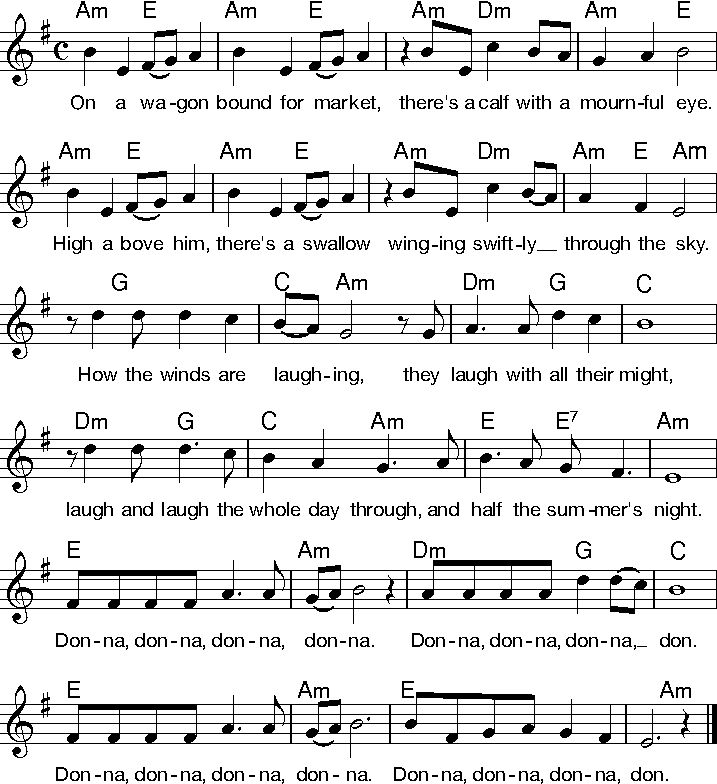
\includegraphics[width=1\textwidth]{Noten/Lied028.pdf}	

\beginverse
\[Am]''Stop com\[E]plaining'', \[Am]said the \[E]farmer. ''\[Am]Who told \[Dm]you a \[Am]calf to \[E]be? 
\[Am]Why can't \[E]you have \[Am]wings to \[E]fly with \[Am]like the \[Dm]swallows so \[Am]proud \[E]and \[Am]free?''
\endverse

\beginchorus
\[G]How the winds are \[C]laugh\[Am]ing, they \[Dm]laugh with \[G]all their \[C]might,
\[Dm]laugh and \[G]laugh the \[C]whole day \[Am]through and \[E]half the \[E7]summer's \[Am]night.
\[E]Donna, donna, donna, \[Am]donna. \[Dm]Donna, donna, \[G]donna, \[C]don.
\[E]Donna, donna, donna, \[Am]donna. \[E7]Donna, donna, donna, \[Am]don.
\endchorus

\beginverse
^Calves are ^easily ^bound and ^slaughtered, ^never ^knowing ^the reason ^why. 
^Whoever ^treasures ^freedom ^like the ^swallow ^has ^learned ^to ^fly.
\endverse

%\renewcommand{\everychorus}{\textnote{\bf Refrain (wdh.)}}
\beginchorus
\[G]How the winds are \[C]laugh\[Am]ing, they \[Dm]laugh with \[G]all their \[C]might,
\[Dm]laugh and \[G]laugh the \[C]whole day \[Am]through and \[E]half the \[E7]summer's \[Am]night.
\[E]Donna, donna, donna, \[Am]donna. \[Dm]Donna, donna, \[G]donna, \[C]don.
\[E]Donna, donna, donna, \[Am]donna. \[E7]Donna, donna, donna, \[Am]don.
\endchorus

\endsong

\beginscripture{}
Das Lied berichtet von der Behandlung der Juden zur Zeit des NS-Regimes. Es handelt von einem Kälbchen, das sich dagegen wehrt, zur Schlachtbank geführt zu werden. „Donna“ kommt vom hebräischen Wort „Adonai“, einer üblichen Anrede Gottes. Das Lied wurde ursprünglich in der jüdischen Sprache für das Musical ''Esterke'' (1941-1942) verfasst.
\endscripture

\begin{intersong}

\end{intersong}
\beginsong{Dort an dem Üferchen}[txt={utta (Gustav Kemperdick)}, mel={russische Volksweise}, bo={86}, pfii={41}, pfiii={19}, index={Kasanka}]

\markboth{\songtitle}{\songtitle}

\beginverse
\endverse

\centering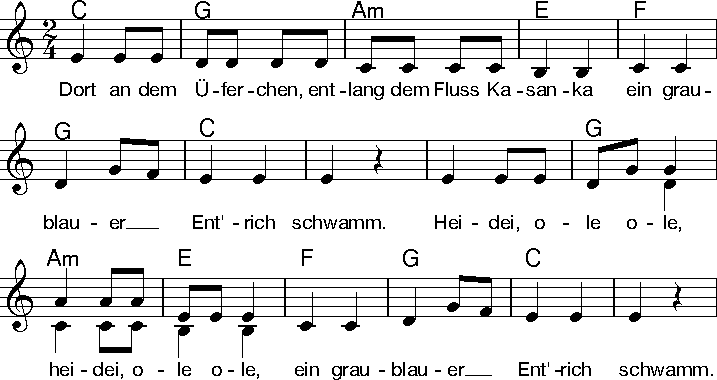
\includegraphics[width=1\textwidth]{Noten/Lied029.pdf}	

\beginverse
\[C]Dort an dem \[G]Üferchen ent\[Am]lang dem Fluss Ka\[E]sanka \[F]ein gar \[G]guter \[C]Bursche ging.
Heidei, o\[G]le ole, \[Am]heidei, o\[E]le ole, \[F]ein gar \[G]guter \[C]Bursche ging.
\endverse

\beginverse
^Sieh, da kommt ein ^Reiter, ^führt ein ledig ^Pferd; der ^Bursch' be^hend hi^nauf sich schwingt.
Heidei, o^le ole, ^heidei, o^le ole, der ^Bursch' be^hend hi^nauf sich schwingt.
\endverse

\beginverse
^Bursch', willst du nicht ^bleiben ^bei der lieben ^Mutter ^und dem ^greisen ^Vater dein? 
Heidei, o^le ole, ^heidei, o^le ole, ^und dem ^greisen ^Vater dein?
\endverse

\beginverse
^Sieh, ich lieb' die ^Mutter ^und den greisen ^Vater, ^doch die bunten ^Mützen der Ko^saken lieb ich mehr.
Heidei, o^le ole, ^heidei, o^le ole, ^doch die bunten ^Mützen der Ko^saken lieb ich mehr.
\endverse

\beginverse
^Dort auf der ^Brücke ^steht ein junges ^Mädchen, ^Tränen ^tropfen ^in den Fluss.
Heidei, o^le ole, ^heidei, o^le ole, ^Tränen ^tropfen ^in den Fluss.
\endverse

\beginverse
^Dort an dem ^Üferchen, ent^lang dem Fluss Ka^sanka, ^reiten zwei ^junge Ko^saken dahin. 
\lrep Heidei, o^le ole, ^heidei, o^le ole, ^reiten zwei ^junge Ko^saken dahin. \rrep
\endverse


\endsong

\beginscripture{}
Die Kasanka ist ein Nebenfluss der Wolga in der Republik Tatarstan im europäischen Teil Russlands. ''Kosaken'' (bedeutet in etwa ''freie Krieger'') waren Gemeinschaften freier Reiterverbände aus flüchtigen russischen und ukrainischen Leibeigenen.
\endscripture

\begin{intersong}

\end{intersong} 
\beginsong{Drei rote Pfiffe}[wuw={H.R. Unger, Herrnstadt/Resetarits, 1979}, bo={198}, index={Im Kreis ihrer Enkel}]

\markboth{\songtitle}{\songtitle}

\beginverse
\endverse

\centering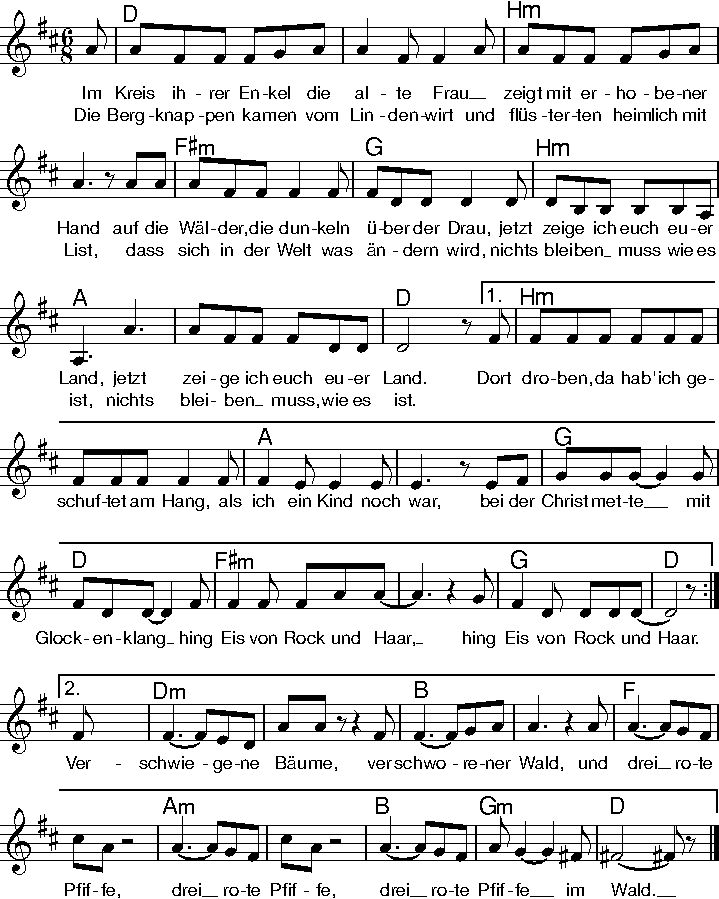
\includegraphics[width=1\textwidth]{Noten/Lied030.pdf}	

\beginverse
Die \[D]Drau hinunter trieb Mond um Mond, es \[Hm]brach der Faschistenkrieg aus.
Da \[F#m]hatte ich einen \[G]Mann an der Front 
und \[Hm]hatte drei Kinder im \[A]Haus, und hatte drei Kinder im \[D]Haus.

Wie \[Hm]tönte da markiger Nazigesang von \[A]deutschem Boden und Blut. 
\[G]Manch ein Bursch' in die \[D]Berge entsprang, 
ich trug \[F#m]Flugblätter unter dem Hut, ich trug \[G]Flugblätter unter dem \[D]Hut.

Der \[D]Gestapo war kalt und der Gauleiter schalt: Parti\[Hm]sanen im eigenen Land!
Ich \[F#m]trug das Geflüster und \[G]Brot in den Wald. 
Sie \[Hm]haben mich Jelka ge\[A]nannt. Sie haben mich Jelka ge\[D]nannt.
\endverse

%\beginchorus
%Ver\[Dm]schwiegene Bäume, ver\[H&]schworener Wald
%Und \[F]drei rote Pfiffe, \[Am]drei rote Pfiffe, \[H&]drei rote \[Gm]Pfiffe im \[D]Wald.
%\endchorus

\beginverse
Der ^Winter war nass und uns wärmte der Hass, viele ^sind's, die die Erde heut' birgt.
Wir ^haben gefochten, dort ^oben am Pass, 
an ^uns'rer Befreiung ge^wirkt, an uns'rer Befreiung ge^wirkt.

Der ^Krieg war vorbei, da war Stille im Land, da ^waren die Lautesten leis'.
Sie ^nahmen das Hitler^bild von der Wand, 
ihre ^Westen, die wuschen sie weiß, ihre ^Westen, die wuschen sie ^weiß.

^Ihr, meine Enkel, was hört ihr so stumm die ^alten, die kalten Berichte?
Jetzt ^trampeln sie wieder auf euren ^Rechten herum, 
er^innert euch meiner Ge^schichte, erinnert euch meiner Ge^schichte.
\endverse

\renewcommand{\everychorus}{\textnote{\bf Refrain (siehe Noten)}}
\beginchorus
\endchorus

\endsong

%\beginscripture{} 
%Die Drau ist ein Nebenfluss der Donau in Südtirol (Italien).
%\endscripture

\begin{intersong}

\end{intersong}
\beginsong{Du machst Kleinholz}[wuw={hussa (Werner Helwig), Wolfgang Held (Nerother Wandervogel), 1955}, bo={98}, pfii={98}, pfiii={52}]

\markboth{\songtitle}{\songtitle}

\beginverse
\endverse

\centering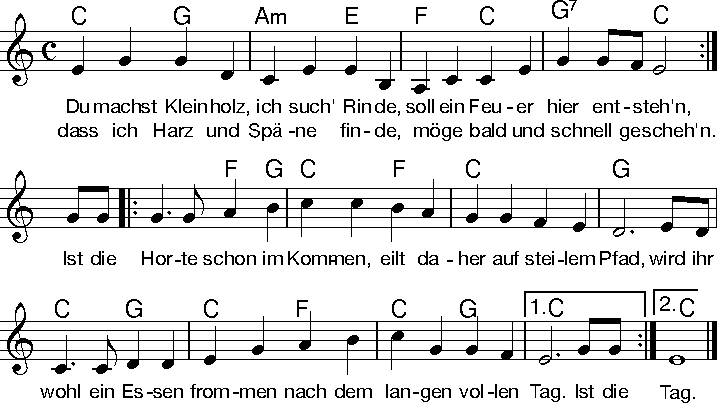
\includegraphics[width=1\textwidth]{Noten/Lied031.pdf}	

\beginverse
\[C]Ich hol' \[G]Wasser, \[Am]du suchst \[E]Schwämme, \[F]leuchten \[C]gelb und \[G]riechen \[C]kalt.
Dass uns \[G]nicht die \[Am]Faulheit \[E]hemme, \[F]geht ein \[C]Regen \[G]durch den \[C]Wald.
\endverse

\beginchorus
Ist die Horte \[G]schon im \[Am]Kommen, \[F]eilt da\[C]her auf steilem \[G]Pfad,
Wird ihr \[C]wohl ein \[G]Essen \[C]frommen, \[F]nach dem \[C]langen, \[G]vollen \[C]Tag.
\endchorus

\beginverse
^Sind das ^Stimmen, ^hörst du ^Rufen? ^Halt die ^Ohren ^in den ^Wind!
Raunt ein ^Bach um ^Felsen^stufen, ^ob das ^wohl die ^Uns'ren ^sind?
\endverse
\renewcommand{\everychorus}{\textnote{\bf Refrain (wdh.)}}
\beginchorus
\endchorus

\endsong

%\beginscripture{} %nix g'fund'n
%\endscripture

\begin{intersong}

\end{intersong}
\beginsong{Edelweißpiraten}[wuw={Herwig Steymans, Hans-Jörg Maucksch}, bo={280}, pfii={70}, pfiii={26}, index={Sie saßen oft am Märchensee}]

\markboth{\songtitle}{\songtitle}

\beginverse
\endverse

\centering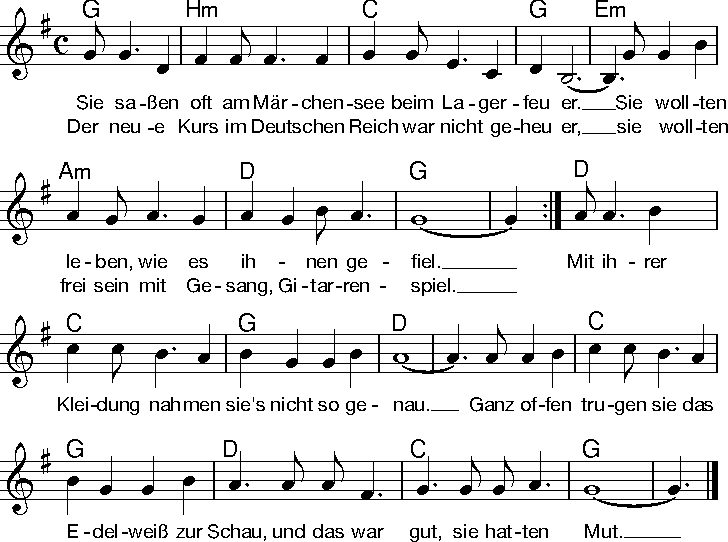
\includegraphics[width=1\textwidth]{Noten/Lied032.pdf}	

\beginverse
\[G]Sie hielten \[Hm]nichts von den \[C]braunen Nazi\[G]horden, \[Em]
sie hielten \[Am]nichts von dem Ge\[D]schrei nach Heil und \[G]Sieg.
\[G]Was war denn \[Hm]bloß aus ihrem \[C]Vaterland ge\[G]worden? \[Em]
Man schürte \[Am]offen den ver\[D]brecherischen \[G]Krieg.
\[D]Da gab's nur \[C]eins zu tun: Be\[G]frei'n wir dieses \[D]Land!
\[D]Da durfte \[C]keiner ruh'n, wir \[G]leisten Wider\[D]stand!
Sie hatten \[C]Mut und das war \[G]gut.\newline
\endverse


\centering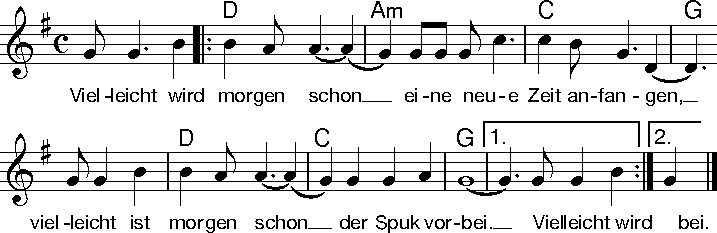
\includegraphics[width=1\textwidth]{Noten/Lied032_1.pdf}	


\beginverse
^Da gab's 'nen ^Güterzug mit ^Kriegsgerät und ^Waffen ^
und was man ^sonst noch braucht für ^einen Völker^mord.
^Sie machten ^sich an den ^Gleisen zu ^schaffen, ^
der Zug er^reichte niemals ^den Bestimmungs^ort.
^Und Essens^marken aus dem ^Parteibüro der ^Stadt
^war'n plötzlich ^weg und Zwangsar^beiter wurden ^satt
und das war ^gut, und das war ^gut.
\endverse

\beginverse
^Sie glaubten ^fest daran, dass ^sie den Sieg er^ringen, ^
sie glaubten ^fest daran, aus ^Schaden wird man ^klug.
^Sie glaubten ^fest daran, als ^sie zum Galgen ^gingen, ^
sie glaubten ^fest daran, als ^man sie vorher ^schlug.
^Und dann die ^Angst, die vor ^jeder Folter ^steht,
^die ist so ^groß, dass man den ^besten Freund ^verrät,
versteht man ^gut, versteht man ^gut.
\endverse

\beginverse
^Sie stehen ^heute noch auf ^manchen schwarzen ^Listen, ^
ich würd' fast ^sagen, es ist ^wieder mal so^weit.
^In Amt und ^Würden sitzen ^immer noch Fa^schisten ^
und zum to^talen Krieg ist ^mancher schnell be^reit.
^Doch seh' ich ^Tausende, und ^das beruhigt mich ^sehr,
^die zeigen ^offen das zer^brochene Ge^wehr,
und das macht ^Mut, und das macht ^Mut.
\endverse

\beginchorus
\lrep Und dann wird \[D]morgen schon\[Am] eine neue \[C]Zeit anfangen\[G]
und dann ist \[D]morgen schon\[C] der Spuk vor\[G]bei. \rrep
\endchorus

\endsong

\beginscripture{}
Die Edelweißpiraten waren eine Gruppe Jugendlicher zur Zeit des Dritten Reichs, die sich der Hitlerjugend nicht anschließen wollten. Als sie weiterhin auf Fahrten gingen, wurden sie von der Gestapo verfolgt und wurden oppositionell politisch. Bis zuletzt wurden Edelweißpiraten, die an einem Abzeichen erkennbar waren, verfolgt und erschossen. Bis heute sind sie nicht als Widerstandsgruppe anerkannt. Dieses Lied reflektiert besonders die Bedeutung der Ehrenfelder Gruppe.
\endscripture

\begin{intersong}

\end{intersong}

\leftwatermark{\put(-48,-586){
\includegraphics{Daumenregister/DaumenregisterA_E}}}
\rightwatermark{\put(351,-585){\includegraphics{Daumenregister/DaumenregisterAL_E}}}

\beginsong{Ein Krampenschlag vor Tag}[wuw={Theodor Kramer, Thomas Fritz, 1934}, bo={356}, index={Was bin ich nur so jäh erwacht}]

\markboth{\songtitle}{\songtitle}

\beginverse
\endverse

\centering\includegraphics[width=1\textwidth]{Noten/Lied033.pdf}	

\beginverse
Vor Schwäche \[Am]dreht es \[G]mich zur \[C]Wand; lang \[G]ist es \[Am]her, schon \[Em]viel zu \[Am]lang,
dass auf dem \[C]Steig ge\[G]spreizt ich \[C]stand bei Nacht und \[Am]selbst den \[Em]Krampen \[Am]schwang.
Die Funken \[F]stoben und wie \[Am]Wein roch scharf der \[F]Grund, das ist vor\[C]bei.
Ein and'rer \[Dm]lockert Stein um \[Am]Stein und weckt mich \[G]vor dem Hahnen\[F]schrei.
\endverse 

\beginverse
Der du vor'm ^Fenster ^stehst, viel^leicht hab' ^ich vor ^Jahren ^dich ge^kannt
und dir die ^Schaufel ^zuge^reicht und hab' dich ^meinen ^Freund ge^nannt.
Das ist vor^bei, lang hungert ^mich. Ich tät' dein ^Werk genauso ^gut.
Und säh' ich ^auf der Straße ^dich, ich zöge ^nicht vor dir den ^Hut.
\endverse

\beginverse
Weißt du, Ge^sell, was ^Hunger ^ist? Und ^weißt du's ^auch, was ^gilt es ^mir!
Den Karren, ^der die ^Erde ^frisst, das Scheit, den ^Krampen ^neid' ich ^dir.
Ich ließ dich ^nicht herein zur ^Tür; du reißt mit ^jedem neuen ^Schlag,
kannst du auch ^zehnmal nichts da^für, mehr als das ^Pflaster auf vor ^Tag.
\endverse

\beginverse
Den tiefen ^Riss, du ^schüttest ^nicht, so^lang du ^lebst, mit ^nichts ihn ^zu.
Am Barren ^schwingt das ^rote ^Licht, die fahlen ^Sterne ^geh'n zur ^Ruh'.
Ein Zug geht ^draußen auf dem ^Steig verhallt der ^letzte Krampen^schlag;
ans Fenster ^schlägt ein schwarzer ^Zweig, mich friert, es ^ist noch lang nicht \[Am]Tag.
\endverse

\endsong

\beginscripture{}
Krampen = Spitzhacke; Das Lied behandelt die Problematik der Arbeitslosigkeit, indem es dem fortwährend Arbeitenden mit der Krampe einen unbeschäftigten, schlaflosen Zuhörer entgegensetzt.
\endscripture

\begin{intersong}

\end{intersong}
\beginsong{Ein stolzes Schiff}[wuw={Erich Schmeckenbecher, Thomas Fritz, Anfang der 1970er Jahre (nach dem Text von Heinrich Schacht von 1828)}, pfii={96}, bo={105}]

\markboth{\songtitle}{\songtitle}

\beginverse
\endverse

\centering\includegraphics[width=1\textwidth]{Noten/Lied033a.pdf}	

\beginverse
Sie zieh'n da\[G]hin auf \[C]blauen Meeres\[G]wogen.
Warum ver\[Am]lassen \[D]sie ihr Heimat\[G]land?
Man hat sie \[G]um ihr \[C]Leben schwer be\[G]trogen,
die Armut \[Am]trieb sie \[D]aus dem Vater\[G]land.
Schauet \[Em]auf, ihr Unter\[C]drücker,
schauet \[Em]auf, ihr Volksbe\[C]trüger,
seht eure \[G]besten Arbeitskräfte \[D]flieh'n,
\[Em]seht, wie sie über's \[C]große \[D]Weltmeer \[G]zieh'n.
\endverse

\beginverse
Sie zieh'n ^dahin, wer ^wagt sie noch zu ^fragen?
Warum ver^lassen ^sie ihr Heimat^land?
Oh, armes ^Deutschland, wie ^kannst du es er^tragen,
dass deine ^Brüder werden ^so ver^bannt?
Was sie ^hofften, hier zu ^gründen,
suchen ^sie dort drüben zu ^finden.
D'rum ziehen ^sie von deutschem Boden ^ab
und ^finden in A^meri^ka ihr ^Grab.
\endverse

\beginverse
Ein stolzes ^Schiff streicht ^einsam durch die ^Wellen,
es führt uns ^uns're ^deutschen Brüder ^fort!
Die Flagge ^weht, die ^weißen Segel ^schwellen,
Ameri^ka ist ^der Bestimmungs^ort.
Seht auf ^dem Verdeck sie stehen,
sich noch ^einmal anzu^sehen,
das ^Vaterland, das ^heimatliche ^Grün,
^seht, wie sie über's ^große ^Weltmeer ^zieh'n.
\endverse

\endsong

\beginscripture{}
Vermutlich geht das Lied auf die Jahre 1848/49 zurück, als, durch wirtschaftliche Not und politischen Druck gezwungen, Zehntausende von Bauern, Handwerkern und Arbeitern nach Amerika auswanderten. Die Folksänger Schmeckenbecher und Fritz (bekannt unter dem Namen Zupfgeigenhansel) entdeckten den unvollständigen, anonymen Text im Deutschen Volksliedarchiv in Freiburg und ergänzten in sinngemäß. Erst 1995 wurde das vollständige Lied mit seiner ursprünglichen, heute kaum noch gesungenen Melodie gefunden.
\endscripture

\begin{intersong}

\end{intersong}
\beginsong{Einheitsfrontlied}[wuw={Bertolt Brecht, Hanns Eisler, 1934}, index={Und weil der Mensch ein Mensch ist}]

\markboth{\songtitle}{\songtitle}

\beginverse
\endverse

\centering\includegraphics[width=1\textwidth]{Noten/Lied033b.pdf}	

\beginverse
Und \[Am]weil der Mensch ein \[E]Mensch ist,
d'rum braucht er auch Kleider und \[Am]Schuh!
Es \[C] macht ihn ein \[Dm]Geschwätz nicht warm
und \[E]auch kein Trommeln \[Am]dazu.
\endverse

\beginchorus
D'rum \[Am]links, zwei, drei! D'rum \[E]links, zwei, drei!
Wo dein \[C]Platz, Genosse \[Dm]ist!
Reih dich ein in die Arbeiter\[Am]einheitsfront, weil du \[E]auch ein Arbeiter \[Am]bist.
\endchorus

\beginverse
Und ^weil der Mensch ein ^Mensch ist,
d'rum hat er Stiefel im Gesicht nicht ^gern!
Er ^will unter sich ^keinen Sklaven seh'n
und ^über sich keinen ^Herr'n.
\endverse
%\renewcommand{\everychorus}{\textnote{\bf Refrain (wdh.)}}



\beginchorus
D'rum \[Am]links, zwei, drei! D'rum \[E]links, zwei, drei!
Wo dein \[C]Platz, Genosse \[Dm]ist!
Reih dich ein in die Arbeiter\[Am]einheitsfront, weil du \[E]auch ein Arbeiter \[Am]bist.
\endchorus

\beginverse
Und ^weil der Prolet ein ^Prolet ist,
d'rum wird ihn kein anderer be^frei'n!
Es ^kann die Befreiung ^der Arbeiter nur
das ^Werk der Arbeiter ^sein.
\endverse



\beginchorus
D'rum \[Am]links, zwei, drei! D'rum \[E]links, zwei, drei!
Wo dein \[C]Platz, Genosse \[Dm]ist!
Reih dich ein in die Arbeiter\[Am]einheitsfront, weil du \[E]auch ein Arbeiter \[Am]bist.
\endchorus


\endsong

\beginscripture{}
Das Lied entstand Ende 1934 für die Erste Internationale Musikolympiade und wurde 1935 in Straßburg uraufgeführt. Es thematisiert Brechts Überzeugung, nur eine Einheitsfront aus Kommunisten und Sozialdemokraten könne den Nationalsozialismus aufhalten.
\endscripture

\begin{intersong}

\end{intersong}
\beginsong{Endlos lang zieht sich die Straße}[wuw={turi (Kurt Kremers), Nerother Wandervogel, 1962}, bo={112}, pfii={32}]

\markboth{\songtitle}{\songtitle}

\beginverse
\endverse

\centering\includegraphics[width=1\textwidth]{Noten/Lied034.pdf}	

\beginverse
\[Em]Auf dem blau\[D]en \[G]Tuch \[D]der \[Em]Blusen \[G]liegt \[D]der \[G]Staub der \[Em]vi\[G]el\[D]en \[Em]Stunden.
\lrep \[Am]Schweigend \[Em]zieht die \[Am]junge \[Em]Horde,
\[G]wei\[D]ter \[G]Weg braucht \[Em]we\[G]n\[D]ig \[Em]Worte. \rrep
\endverse

\beginverse
^Wer kann uns'^re ^We^ge ^messen? ^Wer ^kann ^unser ^Wo^ll^en ^wägen?
\lrep ^Alle, ^die mit ^uns mar^schieren,
^wer^den ^Weg und ^Ziel^ ^er^spüren. \rrep
\endverse

\beginverse
^Neuer Tag ^wird ^Son^ne ^bringen; ^Son^ne ^ruft das ^ju^ng^e ^Leben.
\lrep ^Dunkel ^kann es ^nicht mehr ^halten,
^muss ^zu ^Hohem ^sich^ ^ent^falten. \rrep
\endverse

\endsong

\beginscripture{}
turi (*1920), zuvor Mitglied in einer dem Wandervogel ähnlichen Gruppierung, war im Dritten Reich unter Hitler verbotenerweise weiterhin mit anderen Bündischen auf Fahrt und hatte mehrmals Probleme mit der Gestapo, musste als Moorsaldat in Lagern schuften. Seiner reichskritischen Haltung entsprechend sind auch seine Lieder meist metaphorisch zu verstehen.
\endscripture

\begin{intersong}

\end{intersong}
\beginsong{Es ist an der Zeit}[wuw={Eric Bogle, 1976 (freie deutsche Nachdichtung durch Hannes Wader, 1980)}, pfii={86}, pfiii={43}, index={Weit in der Champagne}]

\markboth{\songtitle}{\songtitle}

\beginverse
\endverse
\centering\includegraphics[width=1\textwidth]{Noten/Lied036.pdf}	

%\centering\includegraphics[width=1\textwidth]{Noten/Lied036_1.pdf}	


\beginverse\memorize
\[G]Hast du, toter Sol\[Em]dat, mal ein \[C]Mädchen ge\[Am]liebt?
Sicher \[D]nicht, denn nur dort, wo es \[G]Frie\[C]den \[G]gibt,
\[G]können Zärtlichkeit \[Em]und Ver\[C]trauen ge\[Am]deih'n.
Warst \[D]Soldat, um zu sterben, nicht \[G]um jung \[D]zu \[G]sein.
Viel\[G]leicht dachtest \[Em]du dir: Ich \[Am]falle schon bald,
nehme \[D7]mir mein Vergnügen, wie es \[G]kommt, mit Ge\[D7]walt.
Dazu \[G]warst du ent\[Em]schlossen, hast \[Am]dich aber dann
vor \[D]dir selber geschämt und es doch \[G]nie \[D]ge\[G]tan.
\endverse

\beginchorus
Ja, auch \[D]dich haben sie schon \[C]genauso \[G]belogen,
so, wie \[D]sie es mit uns heute \[C]immer noch \[G]tun,
und du \[C]hast ihnen alles \[D]gegeben:
Deine \[G]Kraft, deine \[C]Jugend, dein \[D]Le\[G]ben.
\endchorus

\beginverse
^Soldat, gingst du ^gläubig und ^gern in den ^Tod?
Oder ^hast du verzweifelt, ver^bittert, ^ver^roht
^deinen wirklichen ^Feind nicht er^kannt bis zum ^Schluss?
^Ich hoffe, es traf dich ein sau^be^rer ^Schuss.
Oder ^hat ein Ge^schoss dir die ^Glieder zerfetzt?
Hast du ^nach deiner Mutter ge^schrien bis zu^letzt?
Bist du ^auf deinen ^Beinstümpfen ^weitergerannt?
Und ^dein Grab, ^birgt es mehr als ein Bein, ^eine ^Hand?
\endverse
%\renewcommand{\everychorus}{\textnote{\bf Refrain (wdh.)}}

\beginchorus
Ja, auch \[D]dich haben sie schon \[C]genauso \[G]belogen,
so, wie \[D]sie es mit uns heute \[C]immer noch \[G]tun,
und du \[C]hast ihnen alles \[D]gegeben:
Deine \[G]Kraft, deine \[C]Jugend, dein \[D]Le\[G]ben.
\endchorus

\beginverse
^Es blieb nur das ^Kreuz als ^einzige ^Spur
von ^deinem Leben, doch ^hör' mei^nen ^Schwur
^für den Frieden zu ^kämpfen und ^wachsam zu ^sein.
^Fällt die Menschheit noch einmal auf Lü^gen ^he^rein,
dann ^kann es ge^scheh'n, dass bald ^niemand mehr lebt,
niemand, ^der die Milliarden von ^Toten be^gräbt.
Doch längst ^finden sich ^mehr und mehr ^Menschen bereit,
die^sen Krieg zu verhindern, es ist ^an ^der ^Zeit.
\endverse

\beginchorus
Ja, auch \[D]dich haben sie schon \[C]genauso \[G]belogen,
so, wie \[D]sie es mit uns heute \[C]immer noch \[G]tun,
und du \[C]hast ihnen alles \[D]gegeben:
Deine \[G]Kraft, deine \[C]Jugend, dein \[D]Le\[G]ben.
\endchorus

\endsong

\beginscripture{}
Das Lied ist die deutsche Variante von ''The green fields of France'' von Eric Bogle und wurde in dieser Version zu einer Hymne der Friedensbewegung in den 1980er Jahren.
\endscripture

\begin{intersong}

\end{intersong} % 035, 036 getauscht -> Platz
\beginsong{Es führt über den Main}[wuw={Volkslied, 1952 (ergänzt und vertont von Felicitas Kuckuck, 1957)}, bo={118}, pfii={64}]

\markboth{\songtitle}{\songtitle}

\beginverse
\endverse

\centering\includegraphics[width=1\textwidth]{Noten/Lied035.pdf}	

\beginverse
Kommt ein \[Am]Fuhrmann \[G]da\[Am]her, hat ge\[C]laden \[G]gar \[C]schwer.
Seiner \[F]Rösser sind \[G]drei und sie \[C]tanzen vor\[Am]bei,
fallalala\[C]la, fala\[G]la\[Am]la.
\endverse

\beginverse
Kommt ^ein Mädchen ^al^lein auf die ^Brücke ^von ^Stein,
fasst ihr ^Röckchen ge^schwind und sie ^tanzt wie der ^Wind,
fallalala^la, fala^la^la.
\endverse

\beginverse
Kommt ^ein Bursch' oh^ne ^Schuh' und in ^Lumpen ^da^zu.
Als die ^Brücke er ^sah, hei, wie ^tanzte er ^da,
fallalala^la, fala^la^la.
\endverse

\beginverse
Und ^der König ^in Per^son, steigt he^rab von ^seinem ^Thron.
Kaum be^tritt er das ^Brett, tanzt er ^gleich Menu^ett,
fallalala^la, fala^la^la.
\endverse

\beginverse
''Lie^be Leute, ^her^bei, schlagt die ^Brücke ^ent^zwei!''
Und sie ^schwangen das ^Beil, und sie ^tanzten der^weil,
fallalala^la, fala^la^la.
\endverse

\beginverse
Al^le Leute ^im ^Land kommen ^eilig ^ge^rannt: 
''Bleibt der ^Brücke doch ^fern, denn wir ^tanzen so ^gern'',
fallalala^la, fala^la^la.
\endverse

\beginverse
Es ^führt über ^den ^Main eine ^Brücke ^von ^Stein 
und wir ^fassen die ^Händ' und wir ^tanzen ohn' ^End',
fallalala^la, fala^la^la.
\endverse


\endsong

\beginscripture{}
In dem Lied vereint die Brücke Verheißung und Bedrohung auf sich. Weil sie jeden Passanten zum Tanzen zwingt, will der König sie abreißen lassen, was jedoch von den tanzfreudigen Bürgern verhindert werden kann.
\endscripture

\begin{intersong}

\end{intersong}
%\beginsong{The green fields of France}[wuw={Eric Bogle, 1976}, index={Well, how do you do}]

\markboth{\songtitle}{\songtitle}

\beginverse
Well, \[G]how do you \[Em]do, young \[C]Willie Mc\[Am]Bride?
Do you \[D]mind, if I sit here down be\[G]side your \[C]grave\[G]side
and rest for a \[Em]while 'neath the \[D]warm summer \[Am]sun?
I've been \[D]walking all day, and \[G]I'm \[C]nearly \[G]done.
And I see by your \[Em]gravestone you \[C]were only nine\[Am]teen,
when you \[D]joined the great fallen in \[G]nineteen-\[D]sixteen.
Well, I \[G]hope you died \[Em]quick
and I \[Am]hope you died \[C]clean.
Or \[D]Willie McBride, was is it \[G]slow and \[D]ob\[G]scene?
\endverse

\beginchorus
Did they \[D]beat the drum \[D7]slowly,
did they \[C]play the fife \[G]lowly,
did they \[D]sound the dead \[D7]march, as they \[C]lowered you \[D]down,
did the \[C]band play the last post and \[G]cho\[Em]rus,
did the \[G]pipes play the ''\[C]Flowers of the \[D7]Fo\[G]rest''?
\endchorus

\beginverse
And \[G]did you leave a \[Em]wife or a \[C]sweetheart \[Am]behind?
In \[D]some loyal \[D7]heart is your \[C]memory en\[G]shrined.
And though you \[Em]died back in \[C]nineteen-\[Am]sixteen,
to that \[D]loyal \[D7]heart you're for\[C]ever \[G]19.
Or are you a \[Em]stranger without \[C]even a \[Am]name,
for\[D]ever \[C]enshrined behind \[G]some old glass \[D7]pane,
in \[G]an old photo\[Em]graph torn, \[C]tattered and \[Am]stained
and \[D]faded to \[D7]yellow in a \[C]brown leather \[D]frame?
\endverse

\beginverse
The ^sun's shining ^down on these ^green fields of ^France,
the ^warm wind blows ^gently and the ^red poppies ^dance,
the trenches have ^vanished long ^under the ^plow.
No ^gas, no barbed ^wire, no ^guns firing ^now!
But ^here in this ^graveyard it's ^still ''No Man's ^Land'',
the ^countless white ^crosses in ^mute witness ^stand
to ^man's blind ^indifference to ^his fellow man
and a ^whole gene^ration that were ^butchered and ^damned.
\endverse

\beginverse
And I ^can't help but ^wonder, oh ^Willie Mc^Bride.
Do ^all those, who ^lie here, ^know why they ^died,
did you ^really be^lieve them when they ^told you the cause,
did they ^really be^lieve that this ^war would end ^wars?
Well, the ^suffering, the ^sorrow, the ^glory, the ^shame,
the ^killing and ^dying, it ^was all done in ^vain.
Oh ^Willie Mc^Bride, it all ^happened again
and ^again, ^and again, ^and again, ^and again.
\endverse

\endsong

\beginscripture{}
Das Lied beschreibt die Gedanken über ein junges Opfer des Ersten Weltkriegs in Flandern oder Nordfrankreich. Den Daten entsprechend könnte es sich um den in Authuille begrabenen William McBride handeln. Genauso gut könnte es jedoch auch sein, dass das Lied von einer fiktive Person handelt.
\endscripture

\begin{intersong}

\end{intersong} %Es ist an der Zeit: Alles anders machen, Kack Lied!
%\input{Lieder/Lied037a} Nicht hinreichend bekannt, konnte nicht abgetippt werden.
\beginsong{Es liegen drei glänzende Kugeln}[wuw={Franz Joseph Degenhardt, 1963}, bo={126}, pfii={34}, pfiii={15}, index={Drei glänzende Kugeln}]

\markboth{\songtitle}{\songtitle}

\beginverse
\endverse

\centering\includegraphics[width=1\textwidth]{Noten/Lied038.pdf}	

\beginverse
Der \[Am]Wirt, der \[E]hat nur ein \[Am]Auge und \[Dm]das trägt er \[E]hinter dem \[Am]Ohr.
Aus seinem ge\[E]spaltenen \[Am]Kopfe ragt \[Dm]eine An\[E]tenne her\[Am]vor.
Er \[E]trinkt aus einer \[Am]Seele und \[E]ruft aus roter Keh\[E7]le:
\endverse

\beginchorus
\[F]Wer die Kugeln \[C]rollen lässt, \[Dm]daradaradi\[C]dum dei,
\[F]den überkomme die \[C]schwarze Pest, \[E]dara\[E7]daradi\[Am]dum.
\endchorus

\beginverse
Die ^einen ^sagen, die ^Kugeln sind die ^Sonne, die ^Erde, der ^Mond.
Die anderen ^glauben, sie ^seien das ^Feuer, die ^Angst und der ^Tod.
Und ^wenn sie beisammen ^sind, dann ^summen sie in den ^Wind:
\endverse

\renewcommand{\everychorus}{\textnote{\bf Refrain (wdh.)}}
\beginchorus
\endchorus

\beginverse
Und ^dann kam ^einer ge^ritten, es ^war in dem ^Jahr vor der ^Zeit,
auf einer ^gesattelten ^Wolke von ^hinter der ^Ewig^keit.
Er ^nahm von der Wand einen ^Queue, der ^Wirt rief krächzend: ''He, ^he!''
\endverse

\beginchorus
\endchorus

\beginverse
Doch ^jener, der ^lachte zwei ^Donner und ^wachste den ^knöchernen ^Stab,
visierte und ^stieß, und die ^Kugeln prallten ^aneinander, der ^Wirt grub sein ^Grab.
^Fäulnis flatterte ^auf, so ^nahm alles seinen ^Lauf.
\endverse

\beginchorus
\endchorus


\endsong

\beginscripture{}
Das Lied, eines der frühesten Degenhardts, erschien erstmals auf seiner Platte "Zwischen Null Uhr Null und Mitternacht" (1963). Ein Interpretationsansatz geht davon aus, dass in dem Lied das Forschen mit Atomenergie kritisiert wird. So könnten die Kugeln für die Atome stehen, die vom Menschen nicht angestoßen werden sollen, und der verunstaltete Wirt für die möglichen gesundheitlichen Folgen des Experimentierens mit Atomenergie.
\endscripture

\begin{intersong}

\end{intersong}
\beginsong{Es soll sich der Mensch}[txt={nach den „Hayner Dorfmusikanten“, um 1800}, mel={Fiedel Michel, 1978}, bo={130}, pfii={82}, pfiii={44}]

\markboth{\songtitle}{\songtitle}

\beginverse
\endverse

\centering\includegraphics[width=1\textwidth]{Noten/Lied039.pdf}	

\beginverse
Ich \[Am]war ja \[G]so \[C]schrecklich in die \[G]Trina ver\[Am]schossen;
mein Herz war \[G]mit \[C]Zucker und mit \[G]Honig über\[Am]gossen.
Da \[F]kommt doch, zum \[Dm]Teufel, dem \[G]Müller sein \[Am]Franz
\[C]und der \[G]führt \[Am]sie \[G]zum \[Am]Tanz. \[C]Tü-te-\[G]rü-\[Am]tü-\[G]tü-\[Am]tü.
\endverse

\beginverse
Und nun ^schmeckt mir ^kein ^Essen und es ^schmeckt mir kein ^Trinken.
Am liebsten ^da ^würd' ich in der ^Erde ver^sinken.
Ich ^geh auch nicht ^mehr mit die ^anderen ^Knechte,
^denn die ^Men^schen ^sind ^schlechte. ^Tü-te-^rü-^tü-^tü-^tü.
\endverse

\beginverse
Und ^sollt' man ^mit ^solch' Mädchen zum ^Tanze aus^gehen,
ja, dann bleibt man ^am ^besten ganz ^dicht dabei ^stehen,
denn ^sonst tanzen sie ^gleich mit die ^anderen ^Knechte,
^denn solch ^Mäd^chen ^sind ^schlechte. ^Tü-te-^rü-^tü-^tü-^tü.
\endverse

\beginverse
Und ^bin ich ^ge^storben, so ^lasst mich be^graben
und lasst mir ^beim ^Schreiner sechs ^Bretter ab^schaben.
Da^rauf dann zwei ^feurige ^Herzen lasst ^malen,
^denn ich ^kann's ^ja ^be^zahlen. ^Tü-te-^rü-^tü-^tü-^tü.
\endverse

\beginverse
Und ^dann sollt ^ihr ^ein feierlich ^Totenlied ^singen:
Da liegt nun ^der ^Esel in die ^Quer und die ^Längen.
Er ^hat sich ver^plempert mit ^Liebesaf^fären:
^Zu ^Dreck ^soll ^er ^werden! ^Tü-te-^rü-^tü-^tü-^tü.
\endverse

\beginverse
So ^ging das ^zwei ^Wochen und dann ^kam schon die ^Nächste;
vergessen ^all  die ^Sorgen, die ^Ängste, die ^Nöte.
Da ^fing das The^ater von ^vorne ^an;
^man ge^wöhnt ^sich ^da^ran! ^Tü-te-^rü-^tü-^tü-^tü.
\endverse

\endsong

\beginscripture{}
Die 7. Strophe ist aus dem Mittelfränkischen entlehnt und wurde später hinzugefügt.
\endscripture

\begin{intersong}

\end{intersong}
\beginsong{Es war an einem Sommertag}[wuw={Arno Clauss, 1973}, bo={136}, pfii={88}, pfiii={36}]

\markboth{\songtitle}{\songtitle}

\beginverse
\endverse
 
\centering\includegraphics[width=1\textwidth]{Noten/Lied040.pdf}	

\beginverse
Ein \[C]Mann mit \[G]einem \[C]Feder\[G]hut rief: ''\[Am]Männer, \[E]hört mir \[Am]zu!
\[C]Ich ver\[G]sprech' euch \[C]Geld und Gut \[G]und \[Am]Ehre \[E]noch da\[Am]zu.
Der \[G]Kaiser braucht euch, \[C]reiht euch ein, denkt \[G]nicht an Weib und \[C]Haus!
Es \[G]muss ja nicht für \[C]lange sein, zieht \[Am]mit ins \[E]Feld hi\[Am]naus!''

{\nolyrics Zwischenspiel: \[C] \[G] \[C] \[G] \[Am] \[E] \[Am]}
\endverse

\beginverse
Im ^Wirtshaus ^war das ^Trinken ^frei, bezahlt ^mit des ^Kaisers ^Gold.
Und ^während ^dieser ^Zeche^rei trat ^mancher in des ^Kaisers ^Sold.\newpage
Gab ^seiner Braut den ^Abschiedskuss, ver^suchte als Soldat sein ^Glück,
Sah ^nicht des Werbers ^Pferdefuß und ^kam nicht ^mehr zu^rück.
{\nolyrics Zwischenspiel: \[C] \[G] \[C] \[G] \[Am] \[E] \[Am]}
\endverse

\beginverse
Mit ^Flöten^spiel und ^Trommel^schlag ging's ^früh am ^Morgen ^fort.
Die ^Schar ward ^größer, ^denn es ^lag am ^Weg noch ^mancher ^Ort.
Der ^Werber mit dem ^Federhut macht' ^sein Geschäft nicht ^schlecht,
ver^sprach noch vielen ^Geld und Gut, dem ^Kaiser ^dem war's ^recht.
{\nolyrics Zwischenspiel: \[C] \[G] \[C] \[G] \[Am] \[E] \[Am]}
\endverse

\beginverse
Die ^Jahre ^gingen ^in das ^Land und ^von der ^großen ^Schar
war ^keiner, ^der nach ^Hause ^fand, wie ^er ge^gangen ^war.
Der ^eine ließ sein ^Bein im Feld, blind ^kam ein and'rer ^an.
Die ^meisten hatte der ^Tod gefällt, der ^jede ^Schlacht ge^wann.
{\nolyrics Zwischenspiel: \[C] \[G] \[C] \[G] \[Am] \[E] \[Am]}
\endverse

\beginverse
Die ^letzten ^Tränen ^waren ^kaum ge^weint, da ^waren ^sie
auch ^schon ver^gessen, ^wie ein ^Traum; die ^Menschen ^lernen ^nie!
Und ^dann an einem ^Sommertag, irgend^wann und irgend^wo,
da ^tönte wieder ^Trommelschlag, und ^Flöten^spiel klang ^froh.
{\nolyrics Zwischenspiel: \[C] \[G] \[C] \[G] \[Am] \[E] \[Am]}
\endverse

\endsong

\beginscripture{}
%nix g'fund'n
\endscripture

\begin{intersong}

\end{intersong} % 040a, 041 getauscht -> Platz
\beginsong{Es war in einer Regennacht}[wuw={Stan Jones, 1948}, pfii={21}, pfiii={13}]

\markboth{\songtitle}{\songtitle}

\beginverse
\endverse

\centering\includegraphics[width=1\textwidth]{Noten/Lied041.pdf}	

\beginverse
Da \[Em]tritt der Teufel in den Kreis und \[G]winkt dem einen zu;
der \[Em]wendet sich verzweifelt um, beim \[G]Himmel sucht er Ruh'.
\[Em]Zu den Sternen will er flüchten, zur Sonne will er flieh'n,
doch \[C]alle Sterne werden bleich und die \[Em]Sonne \[D]will ver\[Em]glüh'n.
\endverse

\beginchorus
Ji-pi-ei-\[G]jeh - ji-pi-ei-\[Em]joh, \[C]ghostriders in the \[Em]sky.
\endchorus

\beginverse
Da ^öffnet sich der Himmel weit und ^Reiter kommen aus Höh'n
und ^Feuer sprüht aus Pferdenüstern, ^wilde Winde weh'n.
Der ^tote Cowboy wird genommen und keiner wird gefragt
und ^weiter geht es aufwärts in ^wilder, ^toller ^Jagd.
\endverse
%\renewcommand{\everychorus}{\textnote{\bf Refrain (x2)}}
\beginchorus
\lrep Ji-pi-ei-\[G]jeh - ji-pi-ei-\[Em]joh, \[C]ghostriders in the \[Em]sky. \rrep
\endchorus

\endsong

\beginscripture{}
Das Lied heißt im Englischen original ''Ghostriders in the sky'' und wurde durch ein Cover Johnny Cashs bekannt.
\endscripture

\begin{intersong}

\ifthenelse{\boolean{pics}}{
\ThisLRCornerWallPaper{1}{Bilder/Ghostriders_juliane.png}
}{}


\end{intersong}
\beginsong{Es war ein König in Thule}[wuw={Johann Wolfgang von Goethe, K.F.Zelter, 1812}, bo={140}, pfii={48}]

\markboth{\songtitle}{\songtitle}

\beginverse
\endverse

\centering\includegraphics[width=1\textwidth]{Noten/Lied040a.pdf}	

\beginverse
Es \[Am]ging ihm nichts da\[Dm]rü\[Am]ber, er \[Dm]leert' ihn jeden \[E]Schmaus;
\lrep die \[Am]Augen \[G]gingen ihm \[C]ü\[Dm]ber, so \[Am]oft er \[E]trank da\[Am]raus. \rrep
\endverse

\beginverse
Und ^als er kam zu ^ster^ben, zählt' ^er seine Städt' im ^Reich,
\lrep gönnt' ^alles ^seinen ^Er^ben, den ^Becher ^nicht zu^gleich. \rrep
\endverse
 
\beginverse
Er ^saß beim Königs^mah^le, die ^Ritter um ihn ^her,
\lrep auf ^hohem ^Väter^saa^le, dort ^auf dem ^Schloss am ^Meer. \rrep
\endverse

\beginverse
Dort ^stand der alte ^Ze^cher, trank ^letzte Lebens^glut,
\lrep und ^warf den ^heiligen ^Be^cher hi^nunter ^in die ^Flut. \rrep
\endverse

\beginverse
Er ^sah ihn stürzen, ^trin^ken und ^sinken in das ^Meer,
\lrep die ^Augen ^täten ihm ^sin^ken - trank ^nie einen ^Tropfen ^mehr. \rrep
\endverse


\endsong

%\beginscripture{}
%\endscripture

\begin{intersong}

\end{intersong}
\beginsong{Es wollt ein Bauer früh aufstehn}[wuw={Volkslied aus dem 15. Jahrhundert, Fassung von Thomas Fritz und Erich Schmeckenbecher, 1978}, bo={142}, pfii={76}, pfiii={57}]

\markboth{\songtitle}{\songtitle} 


\beginverse
\endverse

\centering\includegraphics[width=1\textwidth]{Noten/Lied042.pdf}

\beginverse
Und \[D]als der Bauer nach Hause kam, und als der Bauer nach \[A]Hause kam,
da wollt er was zu \[D]fressen ham'.
\endverse

\beginchorus
\[A]Fal-te-rie-te-\[D]ra-la-la, \[A]fal-te-rie-te-\[D]ra.
\endchorus

\beginverse
''Ach ^Lieschen, koch mir Hirsebrei, ach Lieschen, koch mir ^Hirsebrei
mit Bratkartoffeln, ^Spiegelei!''
\endverse

\beginverse
Und ^als der Bauer saß und fraß, und als der Bauer ^saß und fraß,
da rumpelt in der ^Kammer was.
\endverse

\beginverse
''Ach ^liebe Frau, was ist denn das? Ach liebe Frau, was ^ist denn das?
Da rumpelt in der ^Kammer was.''
\endverse

\beginverse
''Ach ^lieber Mann, das ist der Wind, ach lieber Mann, das ^ist der Wind,
der raschelt da im ^Küchenspind.''
\endverse

\beginverse
Der ^Bauer sprach: ''Will selber seh'n'', der Bauer sprach: ''Will ^selber seh'n,
will selber in die ^Kammer geh'n.''
\endverse

\beginverse
Und ^als der Bauer in d' Kammer kam, und als der Bauer in d' ^Kammer kam,
zog der Pfaff' die ^Hosen an.
\endverse

\beginverse
''Ach ^Pfaff', was machst in meinem Haus? Ach Pfaff', was machst in ^meinem Haus?
Ich werf dich gleich zum ^Fenster raus.''
\endverse

\beginverse
Der ^Pfaff', der sprach: ''Was ich verricht' '', der Pfaff, der sprach: ''Was ^ich verricht',
dein' Frau, die kann die ^Beichte nicht.''
\endverse

\beginverse
Da ^nahm der Bauer ein' Ofenscheit, da nahm der Bauer ein' ^Ofenscheit
und schlug den Pfaffen, ^bis er schreit.
\endverse

\beginverse
Der ^Pfaffe schrie: ''O Schreck, o Graus!'', der Pfaffe schrie: ''O ^Schreck, o Graus!''
und hing den Arsch zum ^Fenster raus.
\endverse

\beginverse
Da ^kamen die Leut' von nah und fern, da kamen die Leut' von ^nah und fern
und dachten, es sei der ^Morgenstern.
\endverse

\beginverse
Der ^Morgenstern, der war es nicht, der Morgenstern, der ^war es nicht,
es war des Pfaffen ^Arschgesicht.
\endverse

\beginverse
So ^soll es allen Pfaffen geh'n, so soll es allen ^Pfaffen geh'n,
die nachts zu fremden ^Weibern geh'n.
\endverse

\beginverse
Und ^die Moral von der Geschicht', und die Moral von ^der Geschicht':
Trau' nie des Pfaffen ^Arschgesicht!
\endverse

\endsong

\beginscripture{}
Pfaffe ist ein wenig gebrauchtes Wort für einen Pfarrer beziehungsweise einen Geistlichen.
\endscripture

\begin{intersong}

\end{intersong}

\leftwatermark{\put(-48,-586){\includegraphics{Daumenregister/DaumenregisterA_F}}}
\rightwatermark{\put(351,-585){\includegraphics{Daumenregister/DaumenregisterAL_F}}}

\beginsong{Fahren}[wuw={axi (Alexej Stachowitsch), 1970}, bo={54}, pfii={22}, pfiii={53}, index={Der Geist ist müd'}]

\markboth{\songtitle}{\songtitle}

\beginverse
\endverse

\centering\includegraphics[width=1\textwidth]{Noten/Lied043.pdf}	

\beginverse
Schreit \[G]jeder mir die \[Em]Ohren voll vom \[A7]Paradies auf \[D]Erden.
Weiß \[D7]nicht, wen ich be\[G]dauern soll, weiß \[A7]nur: Es wird nicht \[D]wer\[D7]den.
\endverse

\beginchorus
\[G]Trüb hängen Wolken in den Tag, \[C]fahren, ja \[G]fahren!
Wann bricht ein Licht in uns're Plag? \[D]Fa\[D7]hr\[G]en!
\endchorus

\beginverse
Ein ^Rädchen bin ich ^in der Welt, muss ^mich mitunter ^drehen.
Und ^doch, ihr Herr'n, wem's ^nicht gefällt, mag ^mich von hinten ^se^hen!
\endverse
\renewcommand{\everychorus}{\textnote{\bf Refrain (wdh.)}}
\beginchorus
\endchorus

\beginverse
So ^fahr' ich, weil ich ^leben will das ^Freie, Wunder^bare.
Wer ^Tod mir wünscht, der ^leg' mich still; ich ^lebe, weil ich ^fah^re!
\endverse
\renewcommand{\everychorus}{\textnote{\bf Refrain}}
\beginchorus
\[G]Trüb hängen Wolken in den Tag, \[C]fahren, ja \[G]fahren!
Licht bricht durch Dunkel wie ein Schlag. \[D]Fa\[D7]hr\[G]en!
\endchorus

\endsong

\beginscripture{}
%nix g'fund'n
\endscripture

\begin{intersong}

\ifthenelse{\boolean{pics}}{
\ThisLRCornerWallPaper{1}{Bilder/fahren.png}
}{}

\end{intersong}
\beginsong{Flandern in Not}[txt={Elsa Laura von Wolzogen, 1917}, mel={ca. 1917, nach einem Totentanzlied aus dem 16. Jahrhundert}, bo={66}]

\markboth{\songtitle}{\songtitle} 

\beginverse
\endverse

\beginverse
\endverse

\centering\includegraphics[width=1\textwidth]{Noten/Lied044.pdf}	

\beginverse
Der \[Em]Tod reit' auf einem \[H7]lichten \[Em]Schimmel, schön wie ein Cheru\[H7]bin vom \[Em]Himmel,
wenn \[Am]Mädchen \[Em]ihren \[H7]Reigen \[Em]schreiten, will \[Am]er mit \[Em]ihnen im \[H7]Tanze \[Em]gleiten.\newline

\[Am]Falala\[Em]la, \[Am]falala\[Em]la.
\endverse

\beginverse
Der \[Em]Tod kann auch die \[H7]Trommel \[Em]rühren, man kann den Wirbel im \[H7]Herzen \[Em]spüren.
Er \[Am]trommelt \[Em]hell, er \[H7]trommelt \[Em]laut, er \[Am]schlägt auf \[Em]eine \[H7]Toten\[Em]haut.\newline\newpage

Flan\[Am]dern in \[Em]Not! In \[Am]Flandern \[H7]reitet der \[Em]Tod. In Flandern \[Am]rei\[H7]tet der \[Em]Tod.
\endverse

\beginverse
Als ^er den ersten ^Wirbel ge^schlagen, da hat's das Blut vom ^Herzen ge^tragen.
Als ^er den ^zweiten ^Wirbel ^schlug, den ^Landsknecht ^man zu ^Grabe ^trug.\newline

\[Am]Falala\[Em]la, \[Am]falala\[Em]la.
\endverse

\beginverse
Der ^dritte Wirbel ist ^so lang ge^gangen, bis der Landsknecht von Gottes ^Segen em^pfangen.
Der ^dritte ^Wirbel ist ^leis' und ^lind, als ^wiegt eine ^Mutter in ^Schlaf ihr ^Kind.\newline

\[Am]Falala\[Em]la, \[Am]falala\[Em]la.
\endverse

\beginverse
Der ^Tod kann Rappen und ^Schimmel ^reiten, der Tod kann lächelnd im ^Tanze ^schreiten.
Er ^trommelt ^laut, er ^trommelt ^fein: Ge^storben, ge^storben, ge^storben muss ^sein!\newline

Flan\[Am]dern in \[Em]Not! In \[Am]Flandern \[H7]reitet der \[Em]Tod. In Flandern \[Am]rei\[H7]tet der \[Em]Tod.
\endverse

\endsong

\beginscripture{}
1917 versuchten die Alliierten im Ersten Weltkrieg, in Ypern in der belgischen Region Flandern die feindlichen Linien zu durchbrechen. Die ''Dritte Flandernschlacht'' entwickelte sich zur größten Materialschlacht des Krieges.
Das Lied wurde zuerst in der Frontzeitung des Wandervogels veröffentlicht.
\endscripture

\begin{intersong}

\end{intersong}
\beginsong{Foggy dew}[wuw={Canon Charles O'Neill, 1919}, bo={322}, pfii={186}, index={'Twas down the glen}]

\markboth{\songtitle}{\songtitle}

\beginverse 
\endverse

\centering\includegraphics[width=1\textwidth]{Noten/Lied045.pdf}	

\beginverse\memorize
'Twas Brit\[Am]tania bade our \[G]wild geese \[Em]go, that small \[Am]nations \[Dm]might be \[Am]free,
but their lonely graves are by \[G]Sulva's \[Em]waves or the \[Am]shore of the \[Dm]great North \[Am]Sea.
Oh, \[C]had they died by \[G]Peare's \[C]side or had \[Am]fought with \[Em]Cathal \[F]Brugha,
their \[Am]names we would keep where the \[G]fenians \[Em]sleep 'neath the \[Am]shroud of the \[Dm]foggy \[Am]dew.
\endverse

\beginverse
Right ^proudly high over ^Dublin ^Town they ^hung out the ^flag of ^war.
'Twas better to die 'neath an ^Irish ^sky than at ^Sulva or ^Sud El ^Bar.
And ^from the plains of ^Royal ^Meath strong ^men came ^hurrying ^through,
while ^Britannia's Huns with their ^long range ^guns sailed ^in through the ^foggy ^dew.
\endverse

\beginverse
But the ^bravest fell and the ^requiem ^bell rang ^mournful^ly and ^clear
for those who died that ^Easter^tide in the ^springtime ^of the ^year.
And the ^world did gaze in ^deep a^maze at those ^fearless ^men but ^few,
who ^bore the fight, that ^freedom's ^light might ^shine through the ^foggy ^dew.
\endverse

\beginverse
Ah, ^back through the glen I ^rode a^gain and my ^heart with ^grief was ^sore
for I parted then with va^liant ^men, whom ^I never ^shall ^see more.
But ^to and fro in my ^dreams I ^go and I'd ^kneel and ^pray for ^you,
for ^slavery fled, oh ^glorious ^dead, when ^you fell in the ^foggy ^dew.
\endverse

\endsong

\beginscripture{}
Im April 1916 fand in Irland der Osteraufstand statt, währenddessen die Aufständischen die Republik Irland ausriefen. Nach einer Woche schlugen englische Truppen den Aufstand mit Waffengewalt nieder und richteten die Anführer hin. Das Lied fordert die Iren auf, für ihre eigene Unabhängigkeit zu kämpfen, anstatt für England in den Ersten Weltkrieg zu ziehen.
\endscripture

\begin{intersong}

\end{intersong}

\leftwatermark{\put(-48,-586){\includegraphics{Daumenregister/DaumenregisterA_G}}}
\rightwatermark{\put(351,-585){\includegraphics{Daumenregister/DaumenregisterAL_G}}}


\beginsong{Geburtstagslied}[wuw={Aleksander Timofejewski, 1971, letzte Strophe aus studentischen Kreisen; Übersetzung und Nachdichtung: Erik Schellhorn, 1991}, bo={278}, index={Seht die Leute}]

\markboth{\songtitle}{\songtitle}

\beginverse
\endverse

\centering\includegraphics[width=1\textwidth]{Noten/Lied046.pdf}	


\beginverse
Plötzlich \[Am]kommt ein Hubschrauber
und he\[E]raus steigt ein Zaub'rer,
zeigt den Film “Pippi geht auf die \[Am]Walz”.
Zum Ge\[A]burtstag, da wünscht
er mir viel \[Dm]Glück und wie immer
schenkt er \[Am]mir eine \[E]Tonne voll \[Am]Eis.
\endverse

\beginchorus
Und doch, ich \[E]spiele auf der Ga\[Am]moschka,
man sieht mich \[G]auf dem Trotto\[C]ir.
\lrep Aber \[Dm]leider ist Ge\[Am]burtstag
nur ein\[Dm]mal \[E7]im \[Am (A7)]Jahr. \rrep
\endchorus

\beginverse
Ich hab' ^heute Geburtstag,
alle ^kommen am Sonntag,
fröhlich lärmen sie im Haus he^rum.
Und sie ^tanzen, sie singen,
dass die ^Wände mitschwingen,
und zer^stören mein ^Aquari^um.
\endverse

\beginchorus
Oh, wie sie \[E]rauchen und sie ver\[Am]sauen
den Teppich, \[G]der ganz neu noch \[C]war.
\lrep Ach, wie \[Dm]gut, man hat Ge\[Am]burtstag
nur ein\[Dm]mal \[E7]im \[Am (A7)]Jahr. \rrep
\endchorus

\endsong

\beginscripture{}
Dies ist die Übersetzung des ''Liedes des Krokodils Gena'', einer russischen Roman-, Theater- und Zeichentrickfilmfigur.
\endscripture

\begin{intersong}

\end{intersong}
\beginsong{Gospodar}[mel={Rudi Rogoll, 1984}, txt={Theodor Kramer, 1984}, bo={172}, pfiii={64}]

\markboth{\songtitle}{\songtitle}

\beginverse
\endverse

\centering\includegraphics[width=1\textwidth]{Noten/Lied047.pdf}	

\beginverse
\[Am]Treiben wir die \[Dm]Fremden \[Am]über's \[E]Jahr erst \[Am]aus.
\[C]Gospodar, wer glaubst du, \[G]bleibt im Herrschafts\[C]haus?
\lrep \[Am]Werd' ich knechtisch \[Dm]aufsteh'n, \[G7]wo ich mächtig \[C]sitz'?
\[Am]Sind nicht solche \[Dm]Tölpel, \[Am]Bruder \[E]Sliwo\[Am]witz. \rrep
\endverse

\beginverse
^Haben unser ^Herzblut ^nichts für ^nichts ver^tan.
^Alles für die Seinen ^will der Parti^san:
\lrep ^Mutterschaf und ^Lämmer, ^Gänse, Geiß und ^Kitz,
^Kürbis und Me^lonen, ^Mais und ^Sliwo^witz. \rrep
\endverse

\beginverse
^Sind die wilden ^Schweine ^aus dem ^Land ver^jagt,
^die verkohlten Hütten ^aufgebaut und ^ragt
\lrep ^blank im Dorf der ^Maibaum, ^Flattern und Ge^fitz;
^oh, wie wird das ^schön sein, ^Bruder ^Sliwo^witz. \rrep
\endverse

\endsong

\beginscripture{}
Gospodar kommt aus dem slawischen und bedeutet Gaststätte.

Sliwowitz ist ein in Osteuropa verbreiteter Pflaumenbranntwein.
\endscripture

\begin{intersong}

\end{intersong}
\beginsong{Gregor}[txt={aus der Jungenschaft, niedergeschrieben von Eberhard Köbel und Günther Wolff, 1934}, mel={nach ukrainischem Volkslied}, bo={166}, pfii={104}, pfiii={65}, index={Gehe nicht, oh Gregor}]

\markboth{\songtitle}{\songtitle}

\beginverse
\endverse

\centering\includegraphics[width=1\textwidth]{Noten/Lied048.pdf}	

\beginverse
\[Dm]Dort ist auch die eine mit den \[A7]schwarzen Augen\[Dm]brauen.
Glaube mir, oh Gregor, das ist \[A7]eine Zaube\[Dm]rin.
\lrep \[C] \[F]Ihre schmale Hand braut dir \[C]Tee aus Zauber\[F]kräu\[A7]tern,
\[Dm]legt sich über deine Seele \[A7]wie der Herbst auf's \[Dm]Land.\rrep
\endverse

\beginverse
^Sonntag früh beim Glockenläuten ^grub sie aus das ^Kraut,
schnitt es Montag, alle Sünden ^hexte sie hi^nein,
\lrep ^ ^holt' es Dienstag vor, braute ^Zaubertrank aus den ^Kräu^tern,
^Mittwoch Nacht beim Reigentanze ^gab sie ihn Gre^gor.\rrep
\endverse

\beginverse
^Und am Tag darauf am Tage ^war Grischenko ^tot.
Freitag kam voll Leid und Klage ^und beim Abend^rot
\lrep ^ ^trug man ihn zur Ruh' an der ^Grenze an der ^Stra^ße.
^Viele fromme Leute kamen, ^sahen traurig ^zu.\rrep
\endverse

\beginverse
^Viele Knaben, viele Burschen ^klagten um Gre^gor.
Böse Hexe, Zauberhexe, ^schwarze Zauber^frau,
\lrep ^ ^deine Augenbrauen werden ^keinen mehr be^tö^ren,
^nie mehr wird ein zweiter Gregor ^deinen Künsten ^trau'n. \rrep
\endverse


\endsong

\beginscripture{}
Es handelt sich in dem Lied wahrscheinlich lediglich um ein Mädchen, das den geliebten Zigeuner Gregor vergiftet, weil es auf andere Frauen eifersüchtig ist.
\endscripture

\begin{intersong}

\end{intersong}
%\beginsong{Gute Nacht, Freunde}[wuw={Reinhard Mey, 1972}, pfii={181}]

\markboth{\songtitle}{\songtitle}

\beginverse
\endverse

\centering\includegraphics[width=1\textwidth]{Noten/Lied048a.pdf}	

\beginverse
Habt Dank für die Zeit, die ich mit euch verplaudert hab',
und für eure Geduld, wenn's mehr als eine Meinung gab,
dafür, dass ihr nie fragtet, wann ich komm' oder geh',
für die stets off'ne Tür, in der ich jetzt steh'.
\endverse

\beginchorus
Gute Nacht, Freunde, es wird Zeit für mich zu geh'n.
Was ich noch zu sagen hätte, dauert eine Zigarette und ein letztes Glas im Steh'n.
\endchorus

\beginverse
Für die Freiheit, die als steter Gast bei euch wohnt,
habt Dank, dass ihr nie fragt, was es bringt und was es lohnt.
Vielleicht liegt es daran, dass man von draußen meint,
dass in euren Zimmern das Licht wärmer scheint.
\endverse

\endsong

\beginscripture{}
Mey schrieb das Lied unter dem Pseudonym „Alfons Yondraschek“ für das Gesangsduo Inga und Wolf, das damit im Vorentscheid zum Eurovision Song Contest 1972 den vierten Platz belegte. Es kam in den deutschen Charts auf Rang 22.
\endscripture

\begin{intersong}

\end{intersong} %Rausgeworfen! Noten, nicht Traditionell 

\leftwatermark{\put(-48,-586){\includegraphics{Daumenregister/DaumenregisterA_H}}}
\rightwatermark{\put(351,-585){\includegraphics{Daumenregister/DaumenregisterAL_H}}}

\beginsong{Hester Jonas}[mel={Pit Budde, 1977}, txt={Peter Maiwald, 1977}, bo={90}, pfii={110}, index={Dort unten im Gnadental}]

\markboth{\songtitle}{\songtitle}

\beginverse
\endverse

\centering\includegraphics[width=1\textwidth]{Noten/Lied049x.pdf}	

\beginverse
Die \[Dm]Frauen hörten sie mit \[C]lachendem Gesicht;
schön \[Dm]waren Hesters Träume und \[C]schadeten doch \[Dm]nicht. 
Und \[Dm]mittags auf dem Markt, \[C]wo mancher Händler rief,
ge\[Dm]schah, dass um die Jonas mehr \[C]Volk zusammen\[Dm]lief. \newpage
Die \[Dm]Männer zeigten ihr oft \[C]einen schiefen Mund. 
Die \[Dm]besser'n sagten: ''Hester, du \[C]richtest dich zu\[Dm]grund'.''
Des \[Dm]Nachts zum kühlen Gras ka\[C]men sie hungrig doch  
und \[Dm]wollten Hesters Träume und \[C]baten: ''Heute \[Dm]noch.''
\endverse

\beginchorus
Die \[F]Städte werden \[C]fall'n, wo \[Bb]reich nur wenig \[A]sind; 
die \[F]armen Leute \[C]steigen zum \[Bb]Reichtum ohne \[A7]Sünd'.
Und \[Dm]gibt nicht mehr \[C]den Fürst, nicht \[Dm]Bischof und den \[A]Zar 
und \[F]wird nichts sein am \[C]Morgen, wie \[Bb]es am Abend \[A7]war.
\endchorus

\beginverse
Da ^kamen in der Früh' zwei ^Männer aus der Stadt 
und ^schleppten Hester Jonas vor ^einen Magis^trat. 
Da ^war die Red' von Gott, ^da war die Red' von ihr,
da ^war die Red' von Träumen, die ^kränken Mensch und ^Tier.
Und ^quetschten ihr den Hals und ^brachen ihr Gebein;
die ^ganze Stadt hat Tage voll ^Hester Jonas' ^Schrei'n.
Und ^unterschrieb die Schuld mit ^der verkrümmten Hand 
und ^schrie noch lange Träume, bis ^sie das Feuer ^fand.
\endverse
\renewcommand{\everychorus}{\textnote{\bf Refrain (wdh.)}}
%\beginchorus
%\endchorus

\beginverse
Dort \[Dm]unten im Gnadental ge\[C]schah eine Geschicht', 
die \[Dm]hat schön angefangen und \[C]endete so \[Dm]nicht...
\endverse

\endsong

%\beginscripture{}
%Die sogenannte Hexe von Neuss (Ort bei Düsseldorf) - geboren um 1570 - wurde wegen massiven öffentlichen Gerüchten verhaftet und verhört. Man warf der Hebamme und Kräuterheilkundlerin Schadenzauber, den Abfall von Gott und einen Pakt mit dem Teufel vor, was die Hester nach brutaler Folter auch bestätigte. Nach zwischenzeitlicher Flucht wurde sie am 24. Dezember 1935 enthauptet.
%\endscripture

\begin{intersong}

\end{intersong}
\beginsong{Heute hier, morgen dort}[wuw={Hannes Wader, 1972}, bo={180}, pfii={99}, pfiii={29}]

\markboth{\songtitle}{\songtitle}

\beginverse
\endverse

\centering\includegraphics[width=1\textwidth]{Noten/Lied050.pdf}	

\beginverse
Dass man \[C]mich kaum vermisst, schon nach \[F]Tagen ver\[C]gisst,
wenn ich längst wieder \[Am]anderswo \[G]bin,
stört und \[C]kümmert mich nicht, vielleicht \[F]bleibt mein Ge\[C]sicht
doch dem \[Am]ein' oder \[G]and'ren im \[C]Sinn.
\endverse

\beginchorus
Manchmal \[G]träume ich schwer und dann \[F]denk' ich, es \[C]wär'
Zeit zu \[G]bleiben und nun was ganz \[F]and'res zu \[C]tun.
So vergeht Jahr um Jahr und es \[F]ist mir längst \[C]klar,
dass nichts \[Am]bleibt, dass nichts \[G]bleibt, wie es \[C]war.
\endchorus

\beginverse
Fragt mich ^einer, warum ich so ^bin, bleib ich ^stumm,
denn die Antwort da^rauf fällt mir ^schwer.
Denn was ^neu ist, wird alt, und was ^gestern noch ^galt,
stimmt schon ^heut' oder ^morgen nicht ^mehr.
\endverse
\renewcommand{\everychorus}{\textnote{\bf Refrain (wdh.)}}
\beginchorus
\endchorus

\endsong

\beginscripture{}
Die Melodie zu ''Heute hier, morgen dort'' entstammt dem Song ''Indian Summer'' des Musikers Gary Bolstad um 1960. Hannes Wader schrieb zur Melodie, die er in einem Berliner Folkclub aufschnappte, den heute bekannten Text. Gary Bolstad übersetzte 1997 den deutschen Text von Hannes Wader wiederum ins Englische. 
Das Lied knüpft thematisch an das Gefühl in der Wandervogelbewegung an.
\endscripture

\begin{intersong}

\ifthenelse{\boolean{pics}}{
\ThisLRCornerWallPaper{1}{Bilder/heutehier_julian.jpg}
}{}
\end{intersong}
\beginsong{Hier wächst kein Ahorn}[txt={Jooschen Engelke, ca. 1951}, mel={tejo (Walter Scherf), 1951}, bo={182}]

\markboth{\songtitle}{\songtitle}

\beginverse
\endverse

\centering\includegraphics[width=1\textwidth]{Noten/Lied051.pdf}	


\beginverse
\[Em]Hier \[G]wächst der \[D]Thy\[Em]mian, hier \[D]wächst der Ginster\[Em]strauch
und Dornen \[G]wachsen \[A]aus den \[Em]Steinen, \[D]Dornen aus den \[Em]Steinen.
\endverse

\beginchorus
\lrep \[Em]La \[D]lalerala \[Em]la \[D]lalerala \[Em]la, \[D]lalerala \[Em]la. \rrep
\endchorus

\beginverse
^Hier ^wächst der ^Hand^schar, hier ^wächst der Flinten^lauf
und blüh'n wie ^Lilien ^blüh'n im ^Mondlicht, ^Lilien blüh'n im ^Mondlicht.
\endverse
\renewcommand{\everychorus}{\textnote{\bf Refrain (wdh.)}}

\beginchorus
\endchorus

\beginverse
^Und ^morgen ^A^bend und ^wenn der Nachtwind ^weht,
kommt unser ^Gene^ral ge^ritten, ^unser General ge^ritten.
\endverse

\beginchorus
\endchorus

\beginverse
^Und ^bringt uns ^Ra^ki, hej ^ho bogami ^hej,
und bringt uns ^tausend ^Golddu^katen, ^tausend Golddu^katen.
\endverse

\beginchorus
\endchorus

\endsong

\beginscripture{}
Das Lied ist angelehnt an ein Volkslied aus Montenegro.
\endscripture

\begin{intersong}

\end{intersong}

\leftwatermark{\put(-48,-586){\includegraphics{Daumenregister/DaumenregisterA_I}}}
\rightwatermark{\put(351,-585){\includegraphics{Daumenregister/DaumenregisterAL_I}}}

\beginsong{Im Silberbirkenland}[wuw={aus Kanada}, pfii={58}, pfiii={50}]

\markboth{\songtitle}{\songtitle}

\beginverse
\endverse

\centering\includegraphics[width=1\textwidth]{Noten/Lied052.pdf}	

\beginverse
\[Am]Nach dir mein Herz sich sehnt fern von den Bergen;
\[F]Ich kehr' zu \[C]euch zurück, \[G]Hügel des \[C]Nordens.
\endverse

\beginchorus
\[F]Fels säumt den \[C]blauen See;
Ich \[Em]werd' euch wieder\[Am]seh'n.
\lrep \[Am]Bom badi bom bom \rrep \rep{4} \[G]
\endchorus

\beginverse
^Schnell wie ein Silberfisch gleitet mein Rindenboot
^Über den ^Strom dahin ^trägt es mich ^fort.
\endverse
\renewcommand{\everychorus}{\textnote{\bf Refrain (wdh.)}}

\beginchorus
\endchorus

\beginverse
^Hinter dem blauen See bau' ich mein Wigwam
^Dort an der ^Wasserscheid ^ruhig und ^still.
\endverse

%\beginchorus
%\endchorus

\endsong

\beginscripture{}
''Im Silberbirkenland'' stammt von dem kanadischen Indianerlied ''Land of the Silver Birch''. Die genaue Herkunft ist unklar.
\endscripture

\begin{intersong}
\ifthenelse{\boolean{pics}}{
%\centering\includegraphics[width=1\textwidth]{Bilder/imsilberbirkenland_irena.png}
\ThisLLCornerWallPaper{0.95}{Bilder/imsilberbirkenland_irena.png}

}{}


\end{intersong} %Noten, Jakob macht sie noch
\beginsong{In Junkers Kneipe}[wuw={Julia Schäfer, 1936}, bo={212}]

\markboth{\songtitle}{\songtitle}

\beginverse
\endverse

\centering\includegraphics[width=1\textwidth]{Noten/Lied054.pdf}	

\beginverse
Die \[D]alten Zeiten vorüber gleiten und \[A7]draußen tobt die \[D]Nacht.
Und \[D]immer wieder singen wir die Lieder, die \[A7]uns so froh ge\[D]macht.
\endverse

\beginchorus
Ja, wenn die \[G]Klampfen klingen und die \[D]Burschen singen
und die \[A7]Mädchen fallen ein:
\[D]was kann das Leben schöneres geben?
\[A7]Wir wollen glücklich \[D]sein!
\endchorus

\beginverse
\endverse 

\beginverse
Es ^ist so spät schon, der Wirt, der schläft schon, das ^Bier wird langsam ^schal.
Doch ^eh' wir gehen, zum Schlaf uns legen, da ^singen wir noch^mal:
\endverse

\renewcommand{\everychorus}{\textnote{\bf Refrain (wdh.)}}

\beginchorus
\endchorus

\endsong

\beginscripture{}
''In Junkers Kneipe'' war in der Zeit des Nationalsozialismus vor allem in den Widerstandsgruppen bekannt. Die heutige Version ist von einer Gruppe Mülheimer Edelweißpiraten überliefert. Andere Versionen sprechen den Widerstand gegen den Nationalsozialismus offener an. So heißt es in einer Überlieferung ''Wo die Fahrtenmesser blitzen und die Hitlerjungen flitzen und wir Edelweißpiraten schlagen ein...''
\endscripture

\begin{intersong}

\ifthenelse{\boolean{pics}}{
\vspace{30pt}
\centering\includegraphics[width=0.8\textwidth]{Bilder/injunkers_mikesch.jpg}
}{}

\end{intersong} % 053, 054 getauscht -> Platz
\beginsong{In das Dorf}[wuw={aus dem Russischen}, bo={202}, pfii={35}, pfiii={16}]

\markboth{\songtitle}{\songtitle}

\beginverse
\endverse

\centering\includegraphics[width=1\textwidth]{Noten/Lied053.pdf}	

\beginverse
\[H7]Bauern, in den \[Em]Stall die Schweine, \[H7]dem Zigeuner traue nie. \[Em]
\lrep \[Am]Nehmt die Wäsche \[Em]von der Leine, \[H7]rettet euer \[Em]Federvieh! \rrep
\endverse

\beginverse
^Kesselflicker, ^Scherenschleifer ^preisen ihre Künste laut. ^
\lrep ^Geiger spielen ^Korobuschka, ^schon tanzt Sven mit ^seiner Braut.\rrep
\endverse

\beginverse
^Mädchen, die auf ^Heirat warten, ^drängen sich an Maras Stand, ^
\lrep ^denn die Alte ^legt die Karten, ^liest die Zukunft ^aus der Hand.\rrep
\endverse

\beginverse
^Dudelsack quält ^ohne Pause, ^brauner Bär tanzt mit Gebrumm. ^
\lrep ^Spät geht frohes ^Volk nach Hause, ^dunkel liegt das ^Dorf und stumm.\rrep
\endverse

\endsong

\beginscripture{}
Die Melodie stammt vom russischen Motiv ''Korobeiniki''. Dieses ist in der westlichen Welt vor allem durch die ''Type A''-Musik aus Tetris für den Gameboy bekannt.
\endscripture

\begin{intersong}

\end{intersong}

\leftwatermark{\put(-48,-586){\includegraphics{Daumenregister/DaumenregisterA_J}}}
\rightwatermark{\put(351,-585){\includegraphics{Daumenregister/DaumenregisterAL_J}}}

\beginsong{Jalava}[wuw={H. Forger, G. Herrstadt, W. Resetarits in der ''Proletenpassion'', 1976}, bo={346}, pfii={44}, pfiii={22}, index={Von Sonn' und Kessel}]

\markboth{\songtitle}{\songtitle}

\beginverse
\endverse

\centering\includegraphics[width=1\textwidth]{Noten/Lied055.pdf}

\beginverse*
\endverse
\centering\includegraphics[width=1\textwidth]{Noten/Lied055_1.pdf}	

\beginverse
Sie \[Am]dampften ein in Belostrow, wo Schocks von Offi\[E]zieren
die Züge auf dem Grenzbahnhof penibel kontrol\[Am]lieren.
Sie \[Dm]prüfen jegliches Gesicht bei \[Am]ihrer Inspizierung,
doch \[E]sehen sie am Kessel nicht den \[Am]Staatsfeind der Re\[E]gierung.
\[Am]Jalava weiß, worum es geht, und langsam dampft vor\[E]bei
am letzten Posten, der da steht, Lokomotive zwei-neun-\[Am]drei.
\endverse 

\beginchorus
\[Dm]Jalava, du Finne, was \[Am]lachst du gegen den Wind?
Ich \[E]lache, weil meine Sinne \[Am]alle beisammen sind
und \[Dm]weil wir weiterkamen und \[Am]weil der Wind sich dreht\newpage
und \[E]weil mein Heizer von Flammen und \[Am]Dampfkesseln \[E]was ver\[Am]steht.
\[Dm]Jam-pa pam-pa-di-a \[Am]jam-pa pam-pa-di-a \[E]jam-pa pam-pa-di-a \[Am]hey, \[E]hey, \[Am]hey, \[A]hey
\[Dm]Jam-pa pam-pa-di-a \[Am]jam-pa pam-pa-di-a \[E]jam-pa pam-pa-di-a \[Am]hey, \[E]hey, \[Am]hey!
\endchorus

\beginverse
Da ^saust die Grenzstation vorbei, die Birken stehen ^nackt,
die Lokomotive zwei-neun-drei schnauft in erhöhtem ^Takt.
Und ^Jalava lacht in den Wind, in ^den Oktoberregen:
''^Heizer, wenn wir drüben sind, dann ^wird sich was be^wegen.''
Jetzt ^schneidet der Oktoberwind die letzten Äpfel ^an,
die an den kahlen Bäumen sind an der finnischen Eisen^bahn.
\endverse

\beginchorus
\[Dm]Jalava, du Finne, was \[Am]lachst du gegen den Wind?
Ich \[E]lache, weil meine Sinne \[Am]alle beisammen sind
und \[Dm]weil uns die Fahrt in den Bahnhof \[Am]hinter der Grenze führt
und \[E]Vladimir Iljitsch Uljanow, mein \[Am]Heizer, die Flammen schürt.
\[Dm]Jam-pa pam-pa-di-a \[Am]jam-pa pam-pa-di-a \[E]jam-pa pam-pa-di-a \[Am]hey, \[E]hey, \[Am]hey, \[A]hey
\[Dm]Jam-pa pam-pa-di-a \[Am]jam-pa pam-pa-di-a \[E]jam-pa pam-pa-di-a \[Am]hey, \[E]hey, \[Am]hey!
\endchorus

\endsong

\beginscripture{}
Das Jalava-Lied ist das bekannteste Lied der sogenannten Proletenpassion. Diese ist ein politsches Chorwerk aus dem Jahr 1976 mit dem Anspruch, die deutsche (Leidens-)Geschichte aus ihren Anfangstagen zu beschreiben. Das Jalava-Lied selbst beschreibt, wie Lenin vor der Oktoberrevolution, angeblich als Heizer verkleidet, auf einer finnischen Lokomotive über die Grenze nach Sankt Petersburg geschmuggelt wird.
\endscripture

\begin{intersong}

\end{intersong}
\beginsong{Jenseits des Tales}[txt={Börries Freiherr von Münchhausen, vermutlich 1924}, mel={Robert Götz, 1932}, bo={216}, pfii={62}, pfiii={72}]

\markboth{\songtitle}{\songtitle}

\beginverse
\endverse

\centering\includegraphics[width=1\textwidth]{Noten/Lied056.pdf}	

\beginverse
Sie putzten \[D]klirrend am \[A]Geschirr der \[D]Pferde, 
\[A]her tänzel\[D]te die \[A]Marketende\[D]rin
\lrep und \[G]unter'm \[D]Singen \[G]sprach der \[A]Knaben \[D]einer: 
''Mäd\[A]chen, du \[D]weißt, wo ging der \[Em]Kö\[A]nig \[D]hin?'' \rrep
\endverse

\beginverse
Diesseits des ^Tales stand der ^junge ^König 
^und griff die ^feuchte ^Erde aus dem ^Grund,
\lrep sie ^kühlte ^nicht die ^Glut der ^heißen ^Stirne,
sie ^machte ^nicht sein krankes ^Herz ^ge^sund. \rrep
\endverse

\beginverse 
Ihn heilten ^nur zwei knaben^frische ^Wangen
^und ein ^Mund, den ^er sich selbst ver^bot.
\lrep Noch ^fester ^schloss der ^König ^seine ^Lippen
und ^sah hi^nüber in das ^A^bend^rot. \rrep
\endverse

\beginverse
Jenseits des ^Tales standen ^ihre ^Zelte,
^zum roten ^Abend^himmel quoll der ^Rauch.
\lrep Und ^war ein ^Lachen ^in dem ^ganzen ^Heere
und ^jener ^Reiterbube ^lach^te ^auch. \rrep
\endverse

\endsong

\beginscripture{}
Das Lied wird scherzhaft auch ''Lied des schwulen Königs'' genannt. Tatsächlich lehnt sich das Lied wohl jedoch an die Ballade vom Reiterjungen an, in der die Geliebte des Königs sich als Junge getarnt ins Heer schmuggelt, um bei ihm sein zu können.
\endscripture

\begin{intersong}

\end{intersong}
\beginsong{Jerchenkow}[txt={deutsch von peer (Dieter Krolle), 1958}, mel={nach einem ukrainischen Volkslied}, bo={214}, pfii={40}, pfiii={18}, index={Jeden Abend träumt Jerchenkow}]

\markboth{\songtitle}{\songtitle}

\beginverse
\endverse

\centering\includegraphics[width=1\textwidth]{Noten/Lied057.pdf}	

\beginverse*
{\nolyrics Zwischenspiel: \[Dm] \[Am] \[E] \[Am] \rep{2} \[E] \[Am]}
\endverse

\beginverse\memorize
Als der \[Am]Mond stand nachts am Himmel, klopften \[E]wir beim Starosten \[Am]an.
Alles klauten wir dem Lümmel, selbst den \[E]roten Sara\[Am]fan.
\endverse

\beginchorus
Man \[Dm]müsste wieder \[Am]zwei Pistolen \[E]und ein Pferdchen \[Am]haben,
da\[Dm]zu mit einer \[Am]Reiterschar nach \[E]Nischnij Nowgorod \[Am]traben.
Man \[Dm]müsste wieder \[Am]zwei Pistolen \[E]und ein Pferdchen \[Am]haben,
da\[Dm]zu mit einer \[Am]Reiterschar nach \[E]Nischnij Nowgorod \[Am]tr\[E]ab\[Am]en.
\lrep \[Dm] \[Am] \[E] \[Am] \rrep  \[E] \[Am]
\endchorus

\beginverse 
Dreimal ^ritt ich nach Odessa, dreimal ^sah ich Peters^burg
als des Zaren Leibkosaken unter ^Hebnio Sara^tow.
\endverse
\renewcommand{\everychorus}{\textnote{\bf Refrain (wdh.)}}

\beginchorus
\endchorus 


\beginverse
An die ^vielen langen Feste denk' ich ^sehnsuchtsvoll zu^rück;
Vodkafässer, Tanzen, Singen, diese ^Zeit kehrt nie zu^rück.
\endverse

\beginchorus
\endchorus


\endsong

\beginscripture{}
Nischnij (auch: Nischni) Nowgorod = fünftgrößte russische Stadt, Industrie-Metropole; Starost = Vermögen Verwaltender (etwa: Vorsteher);
Die wahren Identitäten Jerchenkows sowie Hebnio Saratows, insofern es sie gibt, sind unbekannt.
\endscripture

\begin{intersong}

\end{intersong}

\leftwatermark{\put(-48,-586){\includegraphics{Daumenregister/DaumenregisterA_K}}}
\rightwatermark{\put(351,-585){\includegraphics{Daumenregister/DaumenregisterAL_K}}}

\beginsong{Kaperslied}[txt={Gottfried Wolters, 1951}, mel={aus Flandern}, bo={12}, pfii={108}, index={Alle, die mit uns auf Kaperfahrt fahren}]

\markboth{\songtitle}{\songtitle}

\beginverse
\endverse

\centering\includegraphics[width=1\textwidth]{Noten/Lied058.pdf}	

\beginverse
\[Em]Alle, die \[H7]Tod und \[Em]Teufel nicht fürchten,
müssen \[H7]Männer mit \[Em]Bärten sein.
\endverse

\beginchorus
\[G]Jan und Hein und Klaas und Pitt,
\[Em]die haben \[H7]Bärte, die haben \[Em]Bärte,
\[G]Jan und Hein und Klaas und Pitt,
\[Em]die haben \[H7]Bärte, die \[Em]fah\[H7]ren \[Em]mit.
\endchorus

\beginverse 
^Alle, die ^Weiber und ^Branntwein lieben,
müssen ^Männer mit ^Bärten sein.
\endverse
\renewcommand{\everychorus}{\textnote{\bf Refrain (wdh.)}}

\beginchorus
\endchorus

\beginverse
^Alle, die ^mit uns das ^Walross schlachten,
müssen ^Männer mit ^Bärten sein.
\endverse

\beginchorus
\endchorus

\beginverse
^Alle, die ^öligen ^Zwieback kauen,
müssen ^Männer mit ^Bärten sein.
\endverse

\beginchorus
\endchorus

\beginverse
^Alle, die ^endlich zur ^Höll' mitfahren,
müssen ^Männer mit ^Bärten sein.
\endverse

\beginchorus
\endchorus

\endsong

\beginscripture{}
%nichts
\endscripture

\begin{intersong}

\end{intersong}
\beginsong{Kaspar}[wuw={Reinhard Mey, 1968}, pfii={94}, pfiii={45}, index={Sie sagten, er käme von Nürnberg her}]

\markboth{\songtitle}{\songtitle}

\beginverse
\endverse

\centering\includegraphics[width=1\textwidth]{Noten/Lied059.pdf}	

\beginverse\memorize
Sein \[Am]Haar in Strähnen und \[D]wirre, sein \[Am]Gang war gebeugt. \[E7]
''Kein \[Am]Zweifel, dieser \[D]Irre ward vom \[Am]Teufel gezeugt.'' \[E7]
Der \[C]Pfarrer reichte ihm einen Krug
voll \[Am]Milch, er sog ihn in einem Zug.
''\[D]Er trinkt nicht vom Ge\[G]schirre, 
den hat die \[C]Wölfin gesäugt,\[E7]  den hat die \[Am]Wölfin gesäugt.''
\endverse

\beginverse
Mein ^Vater, der in ^unserem Ort der ^Schulmeister war, ^
trat ^vor ihn hin, trotz ^böser Worte ^rings aus der Schar. ^
Er ^sprach zu ihm ganz ruhig und
der ^Stumme öffnete seinen Mund
^und stammelte die ^Worte
''Heiße ^Kaspar^, heiße ^Kaspar.''
\endverse 

\beginverse
Mein ^Vater brachte ^ihn ins Haus, ''^Heiße Kaspar.'' ^
Meine ^Mutter wusch ihm ^die Kleider aus ^und schnitt ihm das Haar. ^
Spre^chen lehrte mein Vater ihn,
^lesen und schreiben und es schien,
^was man ihn lehrte, sog ^er in sich auf,
wie ^gierig er war^, wie ^gierig er war.
\endverse

\beginverse
Zur ^Schule gehörte ^derzeit noch das ^Üttinger Feld. ^
Kaspar ^und ich, wir ^pflügten zu zweit, bald war ^alles bestellt. ^
Wir ^hegten und pflegten jeden Keim,
^brachten im Herbst die Ernte ein,
^von den Leuten vermale^deit,
von deren ^Hunden verbellt^, von deren ^Hunden verbellt.
\endverse

\beginverse
Ein ^Wintertag, der ^Schnee war frisch, ^es war Januar. ^
^Meine Mutter rief: ''^Kommt zu Tisch, ^das Essen ist gar.'' ^
Mein ^Vater sagte: ''Appetit'',
ich ^wartete auf Kaspars Schritt,
^mein Vater fragte ^mürrisch: 
''Wo bleibt ^Kaspar^, wo bleibt ^Kaspar?''
\endverse

\beginverse
Wir ^suchten und wir ^fanden ihn auf dem ^Pfad bei dem Feld. ^
Der ^Neuschnee wehte ^über ihn, ^sein Gesicht war entstellt, ^
die ^Augen angstvoll aufgerissen,
^sein Hemd war blutig und zerrissen.
^Erstochen hatten sie ^ihn 
dort am ^Üttinger Feld^, dort am ^Üttinger Feld.
\endverse

\beginverse
Der ^Polizeirat ^aus der Stadt füllte ^ein Formular. ^
''Gott ^nehm' ihn hin in ^seiner Gnad'', sagte ^der Herr Vikar. ^
Das ^Üttinger Feld liegt lang schon brach,
^nur manchmal bell'n mir noch die Hunde nach,
^dann streu' ich ein paar Blumen auf den ^Pfad 
für ^Kaspar^, für ^Kaspar.
\endverse

\endsong

\beginscripture{}
Die Geschichte um Kaspar Hauser (ca. 1812 bis 1833) existiert in vielen verschiedenen Formen. Die Legende besagt, dass er in einer abgedunkelten Zelle von der Außenwelt abgeschnitten aufgezogen wurde, dabei standen ihm nur Grundnahrungsmittel zur Verfügung, sein Besitz umfasste die nötigste Kleidung und ein Schaukelpferd. Als 16-järiger tauchte er 1828 in Nürnberg auf. Daraufhin kursierten Gerüchte, dass Hauser aus dem badischen Fürstenhaus stamme. Der Rest wird in Reinhard Meys Lied erzählt.
\endscripture

\begin{intersong}

\ifthenelse{\boolean{pics}}{
\ThisLRCornerWallPaper{0.8}{Bilder/kaspar_irena.png}
}{}
\end{intersong} 
\beginsong{Komm raus aus deiner Ecke}[index={Die Morgensonne glitzert auf dem See}]

\markboth{\songtitle}{\songtitle}

\beginverse
Die \[E]Morgensonne \[E7]glitzert auf \[A]dem See, 
\[G]in Wipfeln rauscht der Wind, \[D]alles riecht so frisch.
Ich \[E]fühl' mich frei, wenn \[E7]ich ins Leben \[A]geh'.
\[G]Gehöre ich dazu? \[D]Wie kann das besteh'n? 
\[G]Hörst du den Wind?
\[A]Eine neue Zeit be\[C]ginnt.
Und wenn \[D]du's nicht tust, macht's keiner.
\endverse

\beginchorus
Komm \[A]raus aus deiner \[E]Ecke, klatsch \[D]mit uns in die \[F]Hand!
\[G]Hundert \[A]pro den Frieden \[E]bauen mit \[F]Herz und mit Ver\[G]stand.
Komm \[A]her und zieh mit \[E]uns den \[D]Karren aus dem \[F]Sand!
\[G]Hundert \[A]pro die Welt ge\[E]stalten, bist \[F]du dazu be\[G]reit? Yeah! 
\endchorus

\beginverse
Das \[E]Lagerfeuer \[E7]lädt zum Singen \[A]ein,
\[G]ich fühle mich geborgen, \[D]hier bin ich, wer ich bin. 
Komm \[E]setz dich her, du \[E7]bist hier nicht al\[A]lein.
\[G]Gehöre ich dazu? \[D]Wie kann das entsteh'n?
\[G]Hörst du den Wind?
\[A]Eine neue Zeit be\[C]ginnt. 
Und wenn \[D]du's nicht tust, macht's keiner.
\endverse

\renewcommand{\everychorus}{\textnote{\bf Refrain (wdh.)}}
\beginchorus
\endchorus

\beginverse
Das ^Leben wirft so ^viele Fragen ^auf.
^Wir sind in der Kapelle ^und sprechen ein Gebet. 
Du ^schenkst Vertrauen ^und gibst festen ^Halt.
^Gehöre ich dazu? ^Lass sowas entsteh'n.
^Hörst du den Wind?  
^Eine neue Zeit be^ginnt.  
Und wenn ^du's nicht tust, macht's keiner.  
\endverse

\beginchorus
\endchorus

\beginverse*
\[Am]Das sind uns're Fragen, die \[Dm]Antwort fällt so schwer.  
Wer \[F]kann sie mit uns \[G]suchen? Bist \[Am]du dazu be\[E7]reit?
\[Am]Wie wird uns're Zukunft? Ge\[Dm]stalten wir sie fair?  
\[F]Das sind uns're \[G]Fragen. Die \[Am]Antwort fällt so \[E]schwer,  
die fällt so \[E7]schwer.
\endverse

\beginchorus
\endchorus

\endsong

\beginscripture{}
Lagerlied des VCP-Bundeslagers 2006 in Großzerlang im Norden Brandenburgs.
\endscripture

\begin{intersong}

\end{intersong} 


\leftwatermark{\put(-48,-586){\includegraphics{Daumenregister/DaumenregisterA_L}}}
\rightwatermark{\put(351,-585){\includegraphics{Daumenregister/DaumenregisterAL_L}}}


\beginsong{Lagerboogie}[pfii={5}, index={Ich kenn' die Tante Frieda}]

\markboth{\songtitle}{\songtitle}

\beginverse
Ich \[D]kenn' die Tante Frieda, die wohnt im alten \[A]Haus,
und diese Tante Frieda, die kenn' ich ganz \[D]genau.
Mit einem Eimer Wasser putzt sie das ganze \[A]Haus
und was davon noch übrig bleibt, da macht sie Kaffee \[D]draus.
\endverse

\beginchorus
\lrep Jajaja tschu tschu, der Lagerboogie ist unser \[A]Boogie-Woogie. 
Tschu tschu tschu, die Zeit vergeht im \[D]Nu. \rrep
\endchorus

%\centering\includegraphics[width=1\textwidth]{Noten/Lied060.pdf}	

\beginverse
Der \[D]Lehrer in der Schule macht seinen Kindern \[A]klar,
dass Adam und dass Eva aus einer Rippe \[D]war.
Da meldet sich das Fritzchen: ''Herr Lehrer, au, au, \[A]au!
Mir tut die rechte Rippe weh, ich glaub', ich krieg' 'ne \[D]Frau.''
\endverse

\renewcommand{\everychorus}{\textnote{\bf Refrain (wdh.)}}
\beginchorus
\endchorus

\beginverse
Die ^Mutter liegt im Krankenhaus, der Vater im Sing-^Sing.
Die Oma geht mit Negern aus, die Kinder tanzen ^Swing.
Die Tante hat ein Kind gekriegt, man weiß noch nicht von ^wem.
Der Nachbar hat 'nen Schäferhund, vielleicht ist es von ^dem. 
\endverse

\beginchorus
\endchorus

\beginverse
Ja ^neulich in Kentucky, da ist mal was pas^siert,
da hab'n sie 'nen Verbrecher zum Galgenstrick ge^führt.
Nach etwa einer Stunde, da rief doch dieser ^Schuft:
''Zieht doch nicht so feste, ich krieg' ja keine ^Luft!''
\endverse

\beginchorus
\endchorus

\beginverse
Herr ^Meier kam geflogen auf einem Fass Ben^zin,
da dachten die Franzosen, es wär' ein Zeppe^lin.
Sie luden die Kanonen mit Sauerkraut und ^Speck
und schossen dem Herrn Meier die Unterhosen ^weg.
\endverse

\beginchorus
\endchorus

\endsong

\beginscripture{}
Sing-Sing = Hochsicherheitsgefängnis in der Nähe von New York City.
\endscripture

\begin{intersong}

\end{intersong}
\beginsong{Lang war die Reise}[txt={Jörg Ermisch, 1990}, mel={aus Irland}, bo={226}, pfii={109}, pfiii={60}]

\markboth{\songtitle}{\songtitle}

\beginverse
\endverse

\centering\includegraphics[width=1\textwidth]{Noten/Lied061.pdf}	

\beginverse
\[E]Wie oft sah \[H7]ich im Nebel die Hand vor Augen nicht?
Bald \[C#m]klärt sich der \[A]Himmel, 
es ist Land in \[E]Sicht, \[A]es ist Land in \[H7]Sicht.
\endverse

\beginchorus
\lrep \[E]La la \[H7]la la \[C#m]la la la la \[A]la la \[E]la la \[A]la la la la la la \[H7]la la la la \rrep
\endchorus

\beginverse
^Zwei blaue ^Augen waren voller Licht.
Die ^Fahrt geht immer ^weiter, 
es ist Land in ^Sicht, ^es ist Land in ^Sicht.
\endverse

\renewcommand{\everychorus}{\textnote{\bf Refrain (wdh.)}}
\beginchorus
\endchorus

\beginverse
^Seht, wie die ^Sonne durch den Nebel bricht!
Ein ^Meer voller ^Blumen, 
es ist Land in ^Sicht, ^es ist Land in ^Sicht. 
\endverse

\beginchorus
\endchorus

\beginverse
^Wer weiß, ob schon ^morgen eine neue Zeit anbricht?
Die ^Fahrt geht immer ^weiter,
es ist Land in ^Sicht, ^es ist Land in ^Sicht.
\endverse

\beginchorus
\endchorus

\endsong

\beginscripture{}
%nix g'fund'n
\endscripture

\begin{intersong}
\ifthenelse{\boolean{pics}}{
\ThisLRCornerWallPaper{1}{Bilder/langwardiereise.png}
}{}
\end{intersong}
\beginsong{Landeslager Lampenfieber}[txt={Jan Kellner, Björn Naber, Christian Gernand, 2008}, mel={Billy Joel, 1989}, index={Sommer, Sonne, Sonnenschein}]

\markboth{\songtitle}{\songtitle}

\beginverse
\[G]Sommer, Sonne, Sonnenschein,\[D]Rucksack packen, glücklich sein:
\[Em]Landeslager Lampenfieber \[C]in 2008.

\[G]Kothen, Jurten, Küchenzelt, \[D]rein in die Theaterwelt!
\[Em]And're Bünde sind dabei, die \[C]Neugier ist entfacht.

{\nolyrics Zwischenspiel: \[G] \[D] \[Em] \[C]}

\[G]Aufbau, Wiederseh'n,\[D]Stangenholz, Schlange steh'n,
\[Em]Seil vergessen, ganz egal, der \[C]Nachbar leiht's bestimmt.

\[G]Alles steht, Programmbeginn, da \[D]gehen wir gemeinsam hin.
\[Em]Vorhang auf, ein Augenblick, der \[C]dir den Atem nimmt.
\endverse

\beginchorus
\[G]Wir sind hier auf dem \[D]Lala. 
Kommt mit \[Em]ab ins Grüne, Pfadis \[C]auf die Bühne.
\[G]Wir sind hier auf dem \[D]Lala.
Hallo \[Em]Lampenfieber und hier \[C]sind wir wieder. 
\endchorus

\beginverse
^Eintrittskarten, Sommernacht, ^Sippenabend, viel gelacht,
^Lagerfeuer, Abenteuer, ^singen, spielen, Spaß.

^Kostüm, Rampenlicht, ^Peter Pan, Nachtschicht,
^Bauen, proben, ausprobier'n, ^Applaus ist unser Maß.

{\nolyrics Zwischenspiel: ^ ^ ^ ^}

^Bingo spielen, Hajken gehen, ^Fahnen auf den Jurten wehen,
^Tschai kochen, Lieder singen, ^weit bis in die Nacht.

^Zentralverpflegung, Gottesdienst, ^Lagerduschen, Dreck an Jeans,
^Programm-AG, Oasenteam, ^Freunde treffen leicht gemacht.
\endverse

\renewcommand{\everychorus}{\textnote{\bf Refrain (wdh.)}}
\beginchorus
\endchorus

\beginverse
^Pfadis, Rover, Lagerleitung, ^Schirmherrschaft und Lagerzeitung,
^Technik, Einkauf, Sanität, Pro^gramm, Theologie.

^Schauspieler, Regisseur, ^Maskenbildner und Souffleur,
^viele Hände, unser Lager: ^Wir vergessen's nie!

{\nolyrics Zwischenspiel: ^ ^ ^ ^}

^Letzter Abend abgebaut, ^Uraufführung angeschaut,
^müde, dreckig, abgeschlafft, ^die Heimfahrt fast vorbei.

^Ausgeschlafen, denk' zurück: ^Welch ein Lager, was ein Stück,
^Riesenstimmung, nächstes Mal sind ^wir wieder dabei!
\endverse

\beginchorus
\endchorus

\endsong

\beginscripture{}
Lagerlied des Landeslagers des VCP Hessen 2008 in Reinwarzhofen, Mittelfranken.
\endscripture

\begin{intersong}

\end{intersong}
\beginsong{Leinen los}[wuw={Leonie Diedrichs, 2010}]

\markboth{\songtitle}{\songtitle}

\beginchorus
\[C]Leinen los, auf zu \[F]neuen Abenteuern! Volle \[G]Fahrt voraus, auf die \[C]Zukunft zusteuern.
Kommt macht mit und packt \[F]alle mit an, da\[G]mit die Welt sich weiterdrehen \[C]kann.
\endchorus

\beginverse
Hast du dir mal \[G]überlegt, wie's in \[F]100 Jahren \[C]weitergeht? 
Wenn die Kinder deiner Kinder schon er\[G]wachsen sind, 
dann weht auf  \[F]unserer Welt vielleicht ein \[G]anderer Wind.  
\endverse

\renewcommand{\everychorus}{\textnote{\bf Refrain (wdh.)}}
\beginchorus
\endchorus

%\centering\includegraphics[width=1\textwidth]{Noten/Lied061b.pdf}

\beginverse
Aus Norden, Süden, \[G]Osten, Westen sind \[F]wir gekommen, \[C]um zu testen,
wie man die Welt ein Stückchen besser \[G]hinterlässt,
denn wenn das \[F]funktioniert, wird unser \[G]Leben ein Fest.
\endverse


\beginchorus
\endchorus

\beginverse
Nach vorne schau'n und ^weiter denken kann ^and'ren Menschen ^Leben schenken.
Jetzt müssen wir nur allen zeigen, ^wie das geht,
damit die ^Welt sich auch in 100 Jahr'n noch ^weiterdreht.
\endverse


\beginchorus
\endchorus

\endsong

\beginscripture{}
Lagerlied des VCP-Bundeslagers 2010 in Almke bei Wolfsburg.
\endscripture

\begin{intersong}

\end{intersong} %Ohne Noten (Peter)
\beginsong{Leise weht der Wind}[wuw={von einer Großfahrt des BdP ins Belledonne-Massiv, 1983}, bo={228}, pfii={92}, pfiii={28}]

\markboth{\songtitle}{\songtitle}

\beginverse
\endverse

\centering\includegraphics[width=1\textwidth]{Noten/Lied062.pdf}	

\beginverse
\[Hm]Leise weht der Wind über kahlen \[F#m]Steinen,
ein letzter Blick zu\[G]rück, dort liegt nicht das \[A]Glück,
das wir \[Hm]meinen.
Leise weht der Wind über kahlen \[F#m]Steinen,
nur wer den Berg ver\[G]steht, auf den Gipfel \[A]geht,
denn Grenzen gibt es \[Hm]keine.
\endverse

\beginchorus
Vor uns läuft ein \[A]Schweigen auf dem Weg da\[Hm]von
und man gab ihm einen Na\[A]men:
Man nannte es Belle\[Hm]donne.
Der Berg ist wie ein Kö\[A]nig, die Krone ganz aus \[Hm]Eis,
eine Schleppe voller Blu\[A]men, jung und doch ein \[Hm]Greis.
\endchorus

\beginverse
^Leise weht der Wind über Gletscher^seen.
Wie weit werden wir noch ^kommen? Die Kraft ist uns ge^nommen,
doch die Fahrt muss weiter ^gehen.
Leise weht der Wind über Gletscher^seen.
Unser Ziel erreicht, wir ^scherzen, vergessen alle ^Schmerzen,
wenn wir über allem ^stehen.
\endverse
\renewcommand{\everychorus}{\textnote{\bf Refrain (wdh.)}}
\beginchorus
\endchorus

\beginverse
^Leise weht der Wind über's Alltags^leben,
vor uns liegt die ^Stadt, die keine Seele ^hat.
Was ist der Berg da^gegen?
Leise weht der Wind über's Alltags^leben,
ab und zu dreh'n wir uns ^um, doch die Gipfel bleiben ^stumm,
wir möchten gern' mit ihnen ^reden.
\endverse
\renewcommand{\everychorus}{\textnote{\bf Refrain}}
\beginchorus
Vor uns liegt die \[G]Eile der Zivilisa\[Am]tion,
doch wir kehren wie\[G]der
zu uns'rem Freund Belle\[Am]donne.
Er ist wie ein Kö\[G]nig, die Krone ganz aus \[Am]Eis,
eine Schleppe voller Blu\[G]men und der Wind weht \[Am]leis'.
\endchorus

\endsong

\beginscripture{}
Das Belledonne-Massiv ist ein 60km langer Ausläufer der Alpen in Ostfrankreich, das bis in 2.980m Höhe reicht.
\endscripture

\begin{intersong}

\end{intersong}

\leftwatermark{\put(-48,-586){\includegraphics{Daumenregister/DaumenregisterA_M}}}
\rightwatermark{\put(351,-585){\includegraphics{Daumenregister/DaumenregisterAL_M}}}

\beginsong{Marktfrauen, Kinder und Troubadoure}[wuw={rumpel (Andreas Barth), 1992}, bo={270}, pfii={39}, pfiii={49}, index={Scharlatane, eins will ich euch sagen}]

\markboth{\songtitle}{\songtitle}

\beginverse
\endverse

\centering\includegraphics[width=1\textwidth]{Noten/Lied063.pdf}	

\beginverse
\[Em]Sie war’n nicht \[D]lange im \[C]Ne\[D]bel ver\[Em]borgen,
sie hat nicht \[D]lange die \[C]Blind\[D]heit ge\[Em]quält.
\[Em]Sie haben \[D]Einfall um \[C]Ein\[D]fall ge\[Em]boren,
haben \[D]Gefahr und \[C]Frei\[D]heit ge\[Em]wählt.
\lrep Sie sind nicht \[D]feige, \[F]ängstlich und \[Am]klein.
\[Em]Marktfrauen, \[D]Kinder und \[C]Trou\[D]ba\[Em]doure
\[Em]tanzen in \[D]unsere \[C]Zeit \[D]hi\[Em]nein. \rrep
\endverse

\beginverse
^Trotzen der ^Macht, die mit ^Angst ^Menschen ^presste,
die allen ^Mut zu ^fra^gen ver^bannt.
^Feiern in^mitten der ^Ker^ker die ^Feste,
bauen ihr ^Zelt auf ver^bo^tenes ^Land.
\lrep Blumen er^blüh'n im ^grauen Ge^stein.
^Marktfrauen, ^Kinder und ^Trou^ba^doure,
bunter ^Tanz in die ^Welt ^hi^nein. \rrep
\endverse

\endsong

\beginscripture{}
%nix g'fund'n
\endscripture

\begin{intersong}

\end{intersong}
\beginsong{Michel, warum weinest du?}[wuw={Adolf Glasbrenner, vor 1848}, bo={234}, pfiii={71}]

\markboth{\songtitle}{\songtitle}

\beginverse
\endverse

\centering\includegraphics[width=1\textwidth]{Noten/Lied064.pdf}	

\beginverse
\lrep\[Dm]Michel, warum weinest du, \[A]weinest du so \[Dm]sehr? \rrep
\[C]Weil sie mir mein \[F]Geld stibitzen \[B&]und es mir mit \[F]Blut bespritzen,
 \lrep\[B&]da\[Dm]rum \[C]weine ich, \[Dm]weine \[C]ich so \[Dm]sehr. \rrep
\endverse

\beginverse
\lrep^Michel, warum weinest du, ^weinest du so ^sehr? \rrep
^Weil sie mir mein ^Geld verprassen ^und nicht sagen, ^wo sie's lassen,
\lrep^da^rum ^weine ich, ^weine ^ich so ^sehr. \rrep
\endverse

\beginverse
\lrep^Michel, warum weinest du, ^weinest du so ^sehr? \rrep
^Weil ich für diese ^Ungeheuer ^Heeressteuer ^muss versteuern,
\lrep^da^rum ^weine ich, ^weine ^ich so ^sehr. \rrep
\endverse

\beginverse
\lrep^Darum, Michel, weine nun, ^weine nun nicht ^mehr!\rrep
^Wenn du einsiehst ^deine Schwächen, ^können sie dich ^nicht zerbrechen,
\lrep^da^rum ^weine nun, ^weine ^nun nicht ^mehr.\rrep
\endverse

\endsong

\beginscripture{}
Das Lied entstand kurz vor dem Revolutionsjahr 1848. Mit dem ''Michel'' ist der Deutsche Michel gemeint, eine nationale Personifikation aller Deutschen.
\endscripture

\begin{intersong}

\end{intersong}
\beginsong{Miruschka}[wuw={mündlich überliefert}, bo={236}, pfiii={20}]

\markboth{\songtitle}{\songtitle}

\beginverse
\endverse

\centering\includegraphics[width=1\textwidth]{Noten/Lied065.pdf}	

\beginverse
\[F]Seine \[C]gute \[G]Babusch\[C]ka \[F]schenkt ihm \[C]eine \[G]Tschapotsch\[C]ka.
\endverse

\beginchorus
\[Dm]Eine Ko\[Am]sakenmütze, \[E]dass er auf dem \[Am]Kopfe schwitze, \lrep \[E7]denn es ist \[Am]kalt. \rrep
\endchorus

\beginverse
^Eines ^Tages, ^welch ein ^Schreck, ^ach da ^war die ^Tschapka ^weg.
\endverse

\beginverse
^Väter^chen, wo ^ist mein ^Hut? ^Kalter ^Kopf, der ^tut nicht ^gut. 
\endverse

\beginverse
^Traurig ^sucht er ^sie im ^Wald ^und es ^ist schon ^bitter^kalt.
\endverse

\beginverse
^Immer ^kälter ^wird's im ^Tann ^und er ^macht ein ^Feuer ^an.
\endverse

\beginverse
^Vorne ^hat er ^große ^Hitze, ^wenn er ^doch auch ^hinten ^schwitze.
\endverse

\beginverse
^Und so ^macht sich ^Mirusch^mann ^hinter ^sich ein ^Feuer ^an.
\endverse

\beginverse
^Traurig ^starrt er ^in die ^Glut, ^da ge^friert vor ^Schreck sein ^Blut.
\endverse

\beginverse
^Mirusch^ka ist ^hell ent^setzt, ^hinter ^ihm steht ^Meister ^Petz.
\endverse

\beginverse
^Mirusch^ka flieht ^aus dem ^Banne ^und er^klettert ^eine ^Tanne.
\endverse

\beginverse
^Doch der ^Ast zer^bricht mit ^Knall, ^Mirusch^ka kommt ^schwer zu ^Fall.
\endverse

\beginverse
^Auf des ^Bären ^Nase ^drauf, ^der gibt ^seinen ^Geist gleich ^auf.
\endverse

\beginverse
^Mirusch^ka, der ^lachte ^hell: ''^Hei, ich ^hab' mein ^Mützchen^fell.''
\endverse

\endsong

\beginscripture{}
Babuschka = Weib; Tschapotschka = Kappe/Mütze
\endscripture

\begin{intersong}

\end{intersong}
\beginsong{Molly Malone}[wuw={Irisches Volkslied von James Yorkston, 1883}, bo={210}, pfii={205}, index={In Dublin's fair city}]

\markboth{\songtitle}{\songtitle}

\beginverse
\endverse

\centering\includegraphics[width=1\textwidth]{Noten/Lied066.pdf}

\beginverse
She \[C]was a fish\[Am]monger, which \[Dm]was no \[G7]wonder
for \[C]so was her \[Am]father and \[Dm]mother be\[G7]fore.
And they \[C]both wheeled their bar\[Am]row
through \[Dm]streets broad and \[G7]narrow, crying:
\[C]Cockles and \[Am]mussels, a\[C]live, a\[G7]live, \[C]oh!
A\[C]live, alive, \[Am]oh, a\[Dm]live, alive, \[G7]oh! Crying:
\[C]Cockles and \[Am]mussels, a\[C]live, a\[G7]live, \[C]oh!
\endverse

\beginverse
She ^died of a ^fever and ^no one could ^save her
and ^that was the ^end of sweet ^Molly Ma^lone.
But her ^ghost wheels her ^barrow
through ^streets broad and ^narrow, crying:
^Cockles and ^mussels, a^live, a^live, ^oh!
A^live, alive, ^oh, a^live, alive, ^oh! Crying:
^Cockles and ^mussels, a^live, a^live, ^oh!
\endverse

\endsong

\beginscripture{}
Molly Malone, auch bekannt unter dem Titel ''Cockles and Mussels'' („Herzmuscheln und Miesmuscheln“), ist ein bekanntes irisches Volkslied und eine inoffizielle Hymne der Stadt Dublin. Die Ballade erzählt die Geschichte einer schönen Dubliner Fischhändlerin, die in jungen Jahren an nicht näher bestimmtem Fieber stirbt.
Das Lied wurde auch in der Stanley-Kubrick-Verfilmung von ''A Clockwork Orange'' verwendet: In einer der Schlüsselszenen singt ein betrunkener Landstreicher das Lied.
\endscripture

\begin{intersong}

\ifthenelse{\boolean{pics}}{
%\ThisLRCornerWallPaper{0.5}{Bilder/mollymalone.png}
\nobreak
\center\includegraphics[width=0.55\textwidth]{Bilder/mollymalone.png}

}{}

\end{intersong}
\beginsong{Nachts auf dem Dorfplatz}[wuw={turi (Kurt Kremers), 1964}, bo={240}, pfii={116}]

\markboth{\songtitle}{\songtitle}

\beginverse
\endverse

\centering\includegraphics[width=1\textwidth]{Noten/Lied067.pdf}

\beginverse
\[C]Her mit dem Weinkrug \[F]voll zum \[C]Rande, \[G7]trinkt zur Neige, durst'ge \[C]Zecher!
Zigan, spielst du die \[F]Sara\[C]bande, \[C]lockt als Lohn ein gold'ner \[C]Becher.
\endverse

\beginchorus
\[Am]Tom tom tom \[E]tiri \[Am]tom \[E]tom \[Am]tom, \[G]schmetternde Schlägel und \[D]Trommel\[G]ton:
\[F]Tom \[C]tom \[G7]tom tom \[C]tom, schmetternde Schlägel und \[G7]Trommel\[C]ton.
\endchorus
 
\beginverse
^Knöcherne Finger ^alter ^Fetteln ^lesen Zukunft aus den ^Händen,
Pfeife rauchend und ^Tabak ^bettelnd, ^dürre Beine, feiste ^Lenden.
\endverse
\renewcommand{\everychorus}{\textnote{\bf Refrain (wdh.)}}

\beginchorus
\endchorus

\beginverse
^Segelt des Mondes ^stille ^Barke ^über Pinien und Pla^tanen.
Mitternacht wird zur ^Wende^marke, ^lässt den jungen Tag schon ^ahnen.
\endverse

\renewcommand{\everychorus}{\textnote{\bf Refrain}}

\beginchorus
\[Am]Tom tom tom \[E]tiri \[Am]tom \[E]tom \[Am]tom, \[G]leis' werden Schlägel und \[D]Trommel\[G]ton:
\lrep \[F]Tom \[C]tom \[G7]tom tom \[C]tom, leis' werden Schlägel und \[G7]Trommel\[C]ton. \rrep
\endchorus

\endsong

\beginscripture{}
Das Lied ist auch bekannt unter dem Titel ''Die Schenke von Novo Selo''.
\endscripture

\begin{intersong}

\end{intersong}

\leftwatermark{\put(-48,-586){\includegraphics{Daumenregister/DaumenregisterA_N}}}
\rightwatermark{\put(351,-585){\includegraphics{Daumenregister/DaumenregisterAL_N}}}

\beginsong{Nachts steht Hunger starr}[wuw={olka (Erich Scholz), Nerother Wandervogel, 1934}, pfii={120}, pfiii={61}]

\markboth{\songtitle}{\songtitle}

\beginverse
\endverse 

\centering\includegraphics[width=1\textwidth]{Noten/Lied068.pdf}	

\beginverse
\[Am]Ach, dahin ist \[Dm]eine stolze \[Am]Macht,
\[Dm]keine Glocken \[Am]klingen \[E]durch die rote \[Am]Nacht.
\[Am]Postenschritte, \[G]keine Freiheit \[C]mehr,
\[Dm]hinter Stachel\[Am]draht steht \[E]stumm ein müdes \[Am]Heer.
\[Am]Einer singt die \[Em]alten Lieder,
\[F]lockt uns Schwermut und \[C]Sehnsucht aus der Brust,
\[Dm]wild und trotzig \[Am]klingt es wieder,
\[E]im Vergess'nen \[Am]liegt die alte Lust.
\endverse

\beginchorus
\lrep \[Am]Noch fliegt Russlands \[Em]heiliger Adler,
\[F]Mütterchen, unser \[C]Blut gehört nur dir,
\[Dm]mag das rote \[Am]Heer uns auch jagen,
\[E]leuchtend steht noch \[Am]immer das Panier. \rrep
\endchorus

\beginverse
^Und als Heer, das ^keine Heimat ^hat,
^zieh'n wir ausge^wiesen ^nun von Stadt zu ^Stadt.
^Menschen kommen, ^hören unser ^Lied,
^weiter geht die ^Fahrt, der ^Ruhm uns sinnlos ^blüht.
''^Heimat, Heimat!'', ^summen die Chöre,
^tausendfältig ent^steht uns neu dein Bild.
^Glockenläuten, ^uns're Tenöre,
^Orgelbässe ^klingen dumpf und wild.
\endverse

\renewcommand{\everychorus}{\textnote{\bf Refrain (wdh.)}}
\beginchorus
\endchorus

\endsong

\beginscripture{}
Kosaken = Gemeinschaften freier Reiterverbände, zu denen sich flüchtige Russen und Ukrainer, manchmal auch nur Abenteurer oder anderweitig Abtrünnige, in den südlichen Steppengebieten zusammenschlossen;
Das Lied versetzt in die Lage ''weißer'' Kosaken, die durch den Sieg der kommunistischen Revolution ihre russische Heimat verloren und sich in der Fremde singend ihren Lebensunterhalt verdienen müssen. Als Sänger aber auch als Opfer eines brutalen Regimes boten sie sich besonders nach 1933 vielen Bündischen zur Identifikation an.
\endscripture

\begin{intersong}

\end{intersong}
\beginsong{Near to Banbridge Town}[txt={Cathal MacGarvey}, mel={Musik aus dem Irischen, 1726}, bo={242}, pfii={184}, pfiii={10}]

\markboth{\songtitle}{\songtitle}

\beginverse
\endverse

\centering\includegraphics[width=1\textwidth]{Noten/Lied070.pdf}	

\beginverse
As she \[Em]onward sped, \[D]sure I \[G]scratched my \[D]head an I \[Em]looked with a feeling \[D]rare
And I \[Em]say, says I \[Dm]to a \[G]passer-\[D]by: 'Who's the \[Em]maid with the nut-\[D]brown \[Em]hair?'
He \[G]smiled at me and he \[D]says, says he: 'That's the \[Em]gem of Ireland's \[D]crown!
Young \[Em]Rosie McGann \[D]from the \[G]banks of the \[D]Bann, she's the \[Em]star of the Coun\[D]ty \[Em]Down.'
\endverse

\beginchorus
\lrep Oh, from \[G]Bantry Bay up to \[D]Derry Quay and from \[Em]Galway to Dublin \[D]Town,
No maid \[Em]I've seen \[D]like this \[G]brown col\[D]leen, that I \[Em]met in the Coun\[D]ty \[Em]Down. \rrep
\endchorus

\beginverse
At the ^harvest fair ^she'll be ^surely ^there, so I'll ^dress in my sunday ^clothes
With my ^shoes shone bright ^and my ^hat cocked ^right for a ^smile of my nut-^brown ^rose.
No ^pipe I'll smoke, no ^horse I'll yoke, till my ^plough is a rust-coloured ^brown,
Till a ^smiling bride ^by my ^own fire^side sits the ^star of the Coun^ty ^Down.
\endverse

\renewcommand{\everychorus}{\textnote{\bf Refrain (wdh.)}}
\beginchorus
\endchorus

\endsong

\beginscripture{}
Das Lied The Star of the County Down ist eine irische Ballade von Cathal Mac Garvey (1866-1927). Die Melodie ist weitaus älter und bereits im 1726 erschienen Buch ''Music for Allan Ramsay's Collection of Scots Songs'' von Alexander Stuart unter der Bezeichnung Gilderoy dokumentiert. Auf die gleiche Melodie gibt es zahlreiche weitere Lieder.
Das Lied wird vom Standpunkt eines jungen Mannes aus gesungen, der eine junge Frau namens Rose McCann trifft, die als ''Stern der Grafschaft Down'' bezeichnet wird.
\endscripture

\begin{intersong}

\end{intersong} %Ohne Noten (Mikesch)
\beginsong{Near to Banbridge Town (deutsch)}[mel={Musik aus dem Irischen, 1726}, txt={Cathal Mac Garvey}, pfii={30}, pfiii={11}, index={Eines Morgens ging}]

\markboth{\songtitle}{\songtitle}

\beginverse
Eines \[Em]Morgens ging \[D]ich so für mich \[G]hin \[D]im \[Em]Julisonnen\[D]schein,
Den \[Em]Wiesenpfad, \[D]den \[G]Hang hi\[D]nab kam ein \[Em]schönes Mäg\[D]de\[Em]lein.
Und sie \[G]lacht mich an und ich \[D] freu' mich dran und be\[Em]wund're ihr nussbraunes \[D]Haar.
Einer \[Em]lockenden Fee \[D]kam ich \[G]kaum in die \[D]Näh, ganz ver\[Em]wirrt von dem \[D]nussbraunen \[Em]Haar.
\endverse

\beginchorus
\lrep Oh, from \[G]Bantry Bay up to \[D]Derry Quay and from \[Em]Galway to Dublin \[D]Town, 
No maid \[Em]I've seen \[D]like this \[G]brown col\[D]leen, that I \[Em]met in the Coun\[D]ty \[Em]Down. \rrep 
\endchorus

\beginverse
Doch sie \[Em]ging unbeirrt \[D]ihres Weges, \[G]verwirrt \[D]stand ich \[Em]da und nur eins war mir \[D]klar.
Als ein \[Em]Bauer kam, \[D]sprach ich: '\[G]Lieber \[D]Mann, wer ist \[Em]die mit dem nuss\[D]braunen \[Em]Haar?'
Und der \[G]Mann lacht mich an und mit \[D]Stolz sagt er dann: 'Sie ist die \[Em]Perle von Irlands \[D]Kron'!
Uns're \[Em]Rosie McGann \[D]von den \[G]Ufern des \[D]Boyne ist der \[Em]Stern der Land\[D]schaft \[Em]dort.'
\endverse

\renewcommand{\everychorus}{\textnote{\bf Refrain (wdh.)}}
\beginchorus
\endchorus


\beginverse
Doch ich ^sah sie beim Tanz ^unter'm ^Ernte^kranz eines ^Abends im Sommer^kleid.
Dann mit ^schmeichelndem Blick ^ver^sucht' ich mein ^Glück um das ^Herz meiner nuss^braunen ^Maid.
Geb mein ^Wort dafür, keinen ^Pflug ich führ', wird das ^Eisen vom Rost auch ^braun.
Sitzt an ^meinem Herd ^die, die ^ich be^gehrt, strahlt der ^Stern von Coun^ty ^Down.
\endverse
\beginchorus
\endchorus

\endsong

\beginscripture{}
Das Lied ist die deutsche Version der irischen Ballade 'Near to Banbridge Town' von Cathal Mac Garvey aus dem Jahr 1726. 
\endscripture

\begin{intersong}

\end{intersong} 
\beginsong{Nehmt Abschied Brüder}[wuw={Robert Burns (aus dem Schottischen), Übersetzung: Claus Ludwig Laue, zwischen 1759 und 1796}, bo={246}, pfii={2}, pfiii={3}]

\markboth{\songtitle}{\songtitle}

\beginverse
\endverse

\centering\includegraphics[width=1\textwidth]{Noten/Lied071.pdf}	

\beginverse
Die \[C]Sonne sinkt, es \[G]steigt die Nacht, ver\[C]gangen ist der \[F]Tag.
Die \[C]Welt schläft ein und \[G]leis' erwacht der \[F]Nachtigallen \[C]Schlag.
\endverse

\beginchorus
\[F]Der \[C]Himmel wölbt sich \[G]über's Land. \[F]A\[C]de, auf Wieder\[F]seh'n!
Wir \[C]ruhen all in \[G]Gottes Hand. Lebt \[F]wohl, auf Wieder\[C]seh'n! 
\endchorus

\beginverse
So ^ist in jedem ^Anbeginn das ^Ende nicht mehr ^weit.
Wir ^kommen her und ^gehen hin und ^mit uns geht die ^Zeit.
\endverse

\renewcommand{\everychorus}{\textnote{\bf Refrain (wdh.)}}
\beginchorus
\endchorus

\beginverse
Nehmt ^Abschied Brüder, ^schließt den Kreis; das ^Leben ist ein ^Spiel.
Nur ^wer es recht zu ^leben weiß, ge^langt ans große ^Ziel.
\endverse

\beginchorus
\endchorus



\endsong

\beginscripture{}
Auld Lang Syne ist der Titel eines der bekanntesten Lieder im englischsprachigen Raum. Sinngemäß bedeutet der Titel soviel wie 'längst vergangene Zeit'. Es wird in der anglophonen Welt traditionsgemäß zum Jahreswechsel gesungen, um der Verstorbenen des zu Ende gegangenen Jahres zu gedenken. Der deutsche Titel lautet „Nehmt Abschied, Brüder“. In der Pfadfinderbewegung gilt es weltweit als Abschiedslied, das am Ende von Veranstaltungen gesungen wird.

Wegen der Verwendung in der Pfadfinderbewegung wurde das Lied in zahlreiche Sprachen übertragen. Die deutsche Übertragung „Nehmt Abschied, Brüder“ von Claus Ludwig Laue entstand für die Deutsche Pfadfinderschaft Sankt Georg.
\endscripture

\begin{intersong}

\ifthenelse{\boolean{pics}}{
\ThisLRCornerWallPaper{1}{Bilder/nehmtabschied_mikesch.jpg}
}{}

\end{intersong}
\beginsong{Nordwärts}[wuw={Text und Musik: Silke Neumann, 1982}, bo={248}, pfii={60}, pfiii={46}]

\markboth{\songtitle}{\songtitle}

\beginverse
\endverse

\centering\includegraphics[width=1\textwidth]{Noten/Lied072.pdf}	

\beginverse
\[Am]Wollen frei so \[G]wie ein Vogel \[Dm]wiegen uns im \[Am]kalten Wind,
\[C]woll'n den Ruf der \[G]Wildnis hören, \[Am]wenn wir \[Dm]glück\[Em]lich \[Am]sind.
\endverse

\beginverse
^Woll'n durch Moor und ^Sümpfe waten, ^abends legen ^uns zur Ruh'.
^Klampfen sollen ^leis' erklingen, ^singen ^im^mer^zu.
\endverse

\beginverse
^In der Kohte ^brennt ein Feuer, ^füllt uns alle ^mit Bedacht.
^Schlaf senkt sich auf ^uns hernieder, ^doch die ^Wild^nis ^wacht.
\endverse

\beginverse
^Käuzchenschreie, ^Bäume rauschen ^bis zum frühen ^Morgengrau.
^Über ausge^qualmtem Feuer ^strahlt der ^Him^mel ^blau.
\endverse

\beginverse
^Wenn wir wieder ^heimwärts ziehen, ^sehnet jeder ^sich zurück,
^denkt an die ver^gang'nen Fahrten, ^an ver^gang'^nes ^Glück.
\endverse

\beginverse
^Nordwärts, nordwärts ^woll'n wir wieder ^zu den Bergen ^und den Seen,
^dieses Land noch^mal erleben ^und auf ^Fahr^ten ^geh'n.
\endverse


\endsong

\beginscripture{}
%Nüx gefunden
\endscripture

\begin{intersong}
\end{intersong}

 % 071a, 072 getauscht -> Platz
%\beginsong{Nordfahrt}[wuw={Nils Berkey, 2010}, index={Wir ziehen heute gen Norden}]


\markboth{\songtitle}{\songtitle}

\beginverse
\[A]Wir ziehen heu' \[D]gen Norden,
\[E]denn dort liegt un\[A]ser Ziel.
\[A]Wir freuen uns auf \[D]das,
\[E]was uns erwar\[A]ten wird.
\endverse

\beginchorus
\[Em]Und so ziehen wir nach \[C]Småland, \[Em]wo Elche und Wölfe \[C]sind. 
Über \[G]Felsen und Wie\[D]sen an Seen vor\[C]bei, bis zu Stockholms \[Em]Schären. \[C] \[D] \[A] \[E] \[A]
\endchorus

\beginverse
\[A]Das Lager ist \[D]errichtet, 
\[E]die Zelte ste\[A]hen gut.
\[A]Wird uns der Hun\[D]ger plagen? 
\[E]Die Suppe kö\[A]chelt schon.
\endverse

\beginverse
^Viele Tage ^hier verbracht, ^doch da liegt nicht ^das Glück.
^Die Wildnis uns ^schon ruft, ^wir müssen auf Fahr^ten geh'n!
\endverse

\beginverse
^Müde zurück ^gekommen, ^Erholung ist ^angesagt.
^Doch lange wird dies ^nicht dauern, ^denn das Heimweg plagt ^uns doch sehr.
\endverse

\endsong

\beginscripture{}
Meinen guten Freunden Maik Schordn und Tschonnie gewidmet.\newline 

\endscripture

\begin{intersong}

\end{intersong}
\beginsong{Notabene}[wuw={Carl Michael Bellmann, im deutschen von Klabund, zwischen 1740 und 1795}, bo={186}, index={Holt mir Wein aus vollen Krügen}]

\markboth{\songtitle}{\songtitle}

\beginverse
\endverse

\centering\includegraphics[width=1\textwidth]{Noten/Lied073.pdf}	

\beginverse
\[C]Ach, das Leben \[F]lebt sich \[C]lyrisch, \[F]nota\[C]bene, \[G7]wenn man jung ist
\[C]und es duftet \[F]gar ver\[C]führisch, \[F]nota\[C]bene, \[G7]wenn's kein \[C]Dung ist.
\[G7]Ach wie leicht wird hier erreicht doch, \[F]nota\[C]bene, \[G7]ein 'Viel\[C]leicht' noch.
\endverse

\beginverse
^Lasst die Erde ^heiß sich ^drehen, ^nota^bene, ^bis sie kalt ist.
^Deine Liebste ^sollst du ^sehen, ^nota^bene, ^wenn sie ^alt ist.
^Lache, saufe, hure, trabe, ^nota^bene, ^bis zum ^Grabe.
\endverse
 
\endsong

\beginscripture{} 
Nota bene ist eine lateinische und italienische Floskel, die mit „wohlgemerkt“, „merke wohl „beachte wohl“ oder auch „übrigens“ übersetzt werden kann. Sie leitet sich vom lateinischen Verb notare ab, aus dem auch das deutsche Wort 'notieren' entstanden ist.
\newpage
\endscripture

\begin{intersong}


\ifthenelse{\boolean{pics}}{
\vspace{100pt}
\centering\includegraphics[width=0.75\textwidth]{Bilder/wein.png}	
}{}

\end{intersong}
\beginsong{Nun lustig, lustig}[wuw={Werner Helwig}, bo={252}, pfii={75}]

\markboth{\songtitle}{\songtitle}

\beginverse 
\endverse

\centering\includegraphics[width=1\textwidth]{Noten/Lied073a.pdf}

\beginverse
Denn unser \[D]Orden, das ist verdorben, die letzten Saufbrüder sind ge \[A7]storben,
\lrep es lebet  \[D]keiner mehr als ich und  \[A7]du. \rrep  \[D]
\endverse

\beginverse
Schifflein, ^Schifflein, nun tu dich wenden und lass dich hin nach Riga ^senden,
\lrep wohl zu der ^russ'schen Seekaufshandels^stadt.\rrep ^
\endverse

\beginverse
Und auch in ^Polen ist nichts zu holen, man kommt von dort nicht unbe^stohlen,
\lrep in Danzig ^fängt die Sauferei schon ^an.\rrep ^
\endverse

\beginverse
Doch wollen ^wir es noch einmal wagen und wollen fahren nach Kopen^hagen,
\lrep wohl zu der ^dänischen Reichsresi^denz. \rrep ^
\endverse

\beginverse
Dann geht es ^heim, wohl an den Main, denn Frankfurt steckt noch voller Äppel^wein,
\lrep der letzte ^Heller muss versoffen ^sein. \rrep ^
\endverse

\beginverse
Denn wer das ^alles hat gesehen, der kann getrost nach Hause ^gehen
\lrep und nehmen ^sich ein junges ^Weib. \rrep ^
\endverse


\endsong

\beginscripture{}
%Nix gefeunden
\endscripture

\begin{intersong}
\ifthenelse{\boolean{pics}}{
\ThisLRCornerWallPaper{1}{Bilder/nunlustig.png}
}{}

\end{intersong}

\leftwatermark{\put(-48,-586){\includegraphics{Daumenregister/DaumenregisterA_O}}}
\rightwatermark{\put(351,-585){\includegraphics{Daumenregister/DaumenregisterAL_O}}}

\beginsong{On my honour}[wuw={Cindy Dasch, kanadisches Pfadfinderlied, 1993}, pfii={192}, pfiii={4}]

\markboth{\songtitle}{\songtitle}

\centering\includegraphics[width=1\textwidth]{Noten/Lied074.pdf}	

\beginverse
\[C]People don't need to \[Dm]know my name.
If I \[G]hurt someone, then \[C]I'm to blame.
If I \[Am]helped someone, then \[Dm]I helped me,
and \[G]that's the way, that \[C]it \[F]should \[C]be.
\endverse

\beginverse
^I'be tucked away a ^song or two;
If you're ^feeling low, there's ^one for you,
If you ^need a friend, then ^I will come,
There are ^many more, where ^I ^come ^from.
\endverse

\beginverse
^Come with me where the ^fire burns bright,
You can ^even see better in a ^candle's light,
You can ^find more meanings in a ^campfire's glow,
then ^you'll ever get in a ^year ^or ^so.
\endverse

\beginverse
^We've made a promise do ^always keep,
We'll sing '^Day Is Done', be^fore we sleep,
We'll be ^scouts together and ^when we're gone,
they'll ^still be a-trying and a-^singing ^this ^song.
\endverse

\endsong

\beginscripture{}

\endscripture

\begin{intersong}	

\ifthenelse{\boolean{pics}}{
\ThisLRCornerWallPaper{1}{Bilder/onmyhonour.png}
}{}


\end{intersong}   %Bild

\leftwatermark{\put(-48,-586){\includegraphics{Daumenregister/DaumenregisterA_P}}}
\rightwatermark{\put(351,-585){\includegraphics{Daumenregister/DaumenregisterAL_P}}}

\beginsong{Pop my whip}[pfii={185}, pfiii={47}]

\markboth{\songtitle}{\songtitle}

\beginverse
\[Am]Pop my whip and I'll bring the blood, I'll \[G]make my leaders take the mud.
We grab the \[Am]wheels and we turn them round, a \[G]long, long pull and we are hard on \[Am]ground.
\endverse



\beginchorus
\[Am]To me rol, to me rol, to me ride-o, to me \[G]rol, to me rol, to me ride-o,
To me ride-\[Am]o, to me rudio, to me \[G]rol, to me rol, to me ride-\[Am]o.
\endchorus

\beginverse
^On the fourteenth day of October-o
I ^nitched my tears in order-o
To drive the ^hills of Saludio
To ^me rol, to me rol, to me ride-^o.
\endverse

\renewcommand{\everychorus}{\textnote{\bf Refrain (wdh.)}}
\beginchorus
\endchorus

\beginverse
^When I got there, the hills were asleep,
It ^would make a tender hearted persons weep
To her me ^cuss and pop my whip
And ^to see my oxen pull and ^slip.
\endverse
\beginchorus
\endchorus

\beginverse
^When I get home, I'll have revenge,
I ^had my family among my friends,
I'll bit a^dieu to the whip and line
And ^drive no more in the winter^time.
\endverse
\beginchorus
\endchorus

\endsong

\beginscripture{}
%kein sachstand
\endscripture

\begin{intersong}

\end{intersong} % 075, 076 getauscht -> Platz
\beginsong{Papst und Sultan}[wuw={Christian Ludwig Noack, 1789}, bo={62}, pfiii={68}, index={Der Papst lebt herrlich in der Welt}]

\markboth{\songtitle}{\songtitle}

\beginverse
\endverse

\centering\includegraphics[width=1\textwidth]{Noten/Lied075.pdf}	

\beginverse
\[G]Doch nein, er ist ein armer \[D]Wicht, ein holdes Mädchen küsst er \[G]nicht,
\lrep er schläft in seinem \[D]Bett al\[Em]lein: Drum möchte \[C]ich der \[D]Papst nicht \[G]sein. \rrep
\endverse

\beginverse
^Der Sultan lebt in Saus und ^Braus, er wohnt in einem Freuden^haus
\lrep voll wunderschöner ^Mägde^lein: Drum möcht' ich ^wohl der ^Sultan ^sein. \rrep
\endverse

\beginverse
^Doch nein, er ist ein armer ^Mann, denn folgt er seinem Alko^ran,
\lrep so trinkt er keinen ^Tropfen ^Wein: Drum möcht' ich ^auch nicht ^Sultan ^sein. \rrep
\endverse

\beginverse
^Geteilt veracht' ich beider ^Glück und kehr' in meinen Stand zu^rück,
\lrep doch das geh' ich mit ^Freuden ^ein: Halb Sultan ^und halb ^Papst zu ^sein. \rrep
\endverse

\beginverse
^Drum, Mädchen, gib mir einen ^Kuss, denn heut' bin ich dein Sulta^nus!
\lrep Ihr trauten Brüder, ^schenket ^ein, damit ich ^auch der ^Papst kann ^sein! \rrep
\endverse

\endsong

\beginscripture{}
%nix gefunden
\endscripture

\begin{intersong}

\end{intersong} 

\leftwatermark{\put(-48,-586){\includegraphics{Daumenregister/DaumenregisterA_R}}}
\rightwatermark{\put(351,-585){\includegraphics{Daumenregister/DaumenregisterAL_R}}}

\beginsong{Roter Mond}[wuw={Anja Klenkaus dem Hortenring Ernsthofen (Schwedenfahrt), 1980}, bo={266}, pfii={90}, pfiii={27}]

\markboth{\songtitle}{\songtitle}

\beginverse
\endverse

\centering\includegraphics[width=1\textwidth]{Noten/Lied078.pdf}	

\beginverse
\[Em]Sterne steh'n \[D]hell am Firmament, \[Em]solche Nacht \[D]findet nie ein End'.
\lrep \[G]Dieses Land, \[D]wild und schön, und \[Am]wir dürfen seine \[Em]Herrlichkeit seh'n. \rrep
\endverse

\beginverse
^Rauher Fels, ^Moos und Heidekraut, ^weit entfernt ^schon der Morgen graut.
\lrep ^Fahne weht, ^weiß und blau, das ^Gras schimmert unterm ^Morgentau. \rrep 
\endverse

\beginverse
\[Em]Fahrt vorbei, \[D]morgen geht es fort. \[Em]Kommen wir \[D]wieder an den Ort?
\[G]Norden ist \[D]unser Glück und \[Am]in uns bleibt nur die Er\[Em]innerung zurück.
\[G]Norden ist \[D]unser Glück und \[Am]wir wünschen uns ein \[Em]neues zurück.
\endverse

\endsong

\beginscripture{}
Dieses Lied ist 1980 bei einem Pfadfinderlager des Hortenring Ernsthofen in Schweden entstanden. Die Farben "weiß und blau" beziehen sich auf das Banner des Pfadfinderbundes. Dieser Bund wurde Ende der Neunziger Jahre aufgelöst.
Wenn der Mond nah am Horizont steht, dann wird das Licht so durch die Atmosphäre gefiltert, dass er rot erscheint.
\endscripture 

\begin{intersong}

\end{intersong} % 077, 078 getauscht -> Platz
\beginsong{Raubritter}[wuw={nathan (Georg Hausmann) und anti (Volker Hausmann), Nerother Wandervogel, 1967}, bo={344}, pfii={16}, pfiii={6}, index={Von der Festung dröhnt}]

\markboth{\songtitle}{\songtitle}

\beginverse
\endverse

\centering\includegraphics[width=1\textwidth]{Noten/Lied077.pdf}	 

\beginverse
\[Am]In uns'rer Knechtschaft \[F]Zeit griffen wir zu \[Am]Waffen,
schlugen uns're \[F]Herr'n, Grafen und auch \[Am]Pfaffen.
\endverse

\beginchorus
\[G]Be\[C]herrschen dies Ge\[G]biet, \[Am]singen stolz ihr \[E]Lied: 
\[Am]Raubritter, Raubritter, wie weit \[G]ist \[C]un\[G]ser \[Am]Land?
\[F]Raubritter, Raubritter, wie stark \[C]ist \[F]uns'\[G]re \[Am]Hand?
\endchorus
 
\beginverse
^Groß ist uns're ^Macht, solange wir ^vereint.
Hüten uns're ^Burg, trotzen jedem ^Feind.
\endverse

\renewcommand{\everychorus}{\textnote{\bf Refrain (wdh.)}}
\beginchorus
\endchorus

\endsong

\beginscripture{}
Im Jahre 1967 spaltete sich der Orden der Raubritter vom Orden der Rabenklaue im Nerother Wandervogel ab. Das Lied wurde das Ordenslied des neu gegründeten Ordens. Es existieren viele Textvariationen, die vermutlich durch die mündliche Übetragung entstanden sind.

Als Raubritter bezeichnet man diejenigen Angehörigen des ritterlichen Standes, die sich durch Straßenraub, Fehden und Plünderungszüge bereicherten.
\endscripture

\begin{intersong}

\ifthenelse{\boolean{pics}}{
\ThisLRCornerWallPaper{1}{Bilder/raubritter_mikesch.jpg}
}{}

\end{intersong}
\beginsong{Roter Wein im Becher}[wuw={Helmut König, Musik nach einem französischen Volkslied}, bo={268}, pfii={15}, pfiii={9}]

\markboth{\songtitle}{\songtitle}

\beginverse
\endverse

\centering\includegraphics[width=1\textwidth]{Noten/Lied079.pdf}	

\beginverse
\[Em]Morgens bricht die Runde zu \[D7]neuen Fahrten \[G]auf.
Es \[D7]klingt in aller \[G]Mun\[Am]de ein \[Em]frohes \[H7]Liedchen \[Em]auf. 
\endverse

\beginchorus
\lrep Radi, radi, ra-\[C]di rala\[G]la, \[D7]radi, radi, \[Em]ra-di \[H7]ralala\[Em]la. \rrep
\endchorus

\beginverse
^Steine, Staub und Dornen sind ^schwerlich Tippe^lei.
Wir ^müssen uns an^spor^nen, die ^Qual ist ^bald vor^bei.
\endverse

\renewcommand{\everychorus}{\textnote{\bf Refrain (wdh.)}}
\beginchorus
\endchorus
\beginverse
^Treffen wir uns wieder, der ^Zufall nennt den ^Ort,
so ^schallen uns're ^Lie^der in ^weite ^Ferne ^fort.
\endverse
\beginchorus
\endchorus

\endsong

\beginscripture{}
Tippelei = Walz, Gesellenwanderung
\endscripture

\begin{intersong}

\ifthenelse{\boolean{pics}}{
\vspace{60pt}
\centering\includegraphics[width=0.6\textwidth]{Bilder/roterwein_irena.png}	
}{}

\end{intersong}

\leftwatermark{\put(-48,-586){\includegraphics{Daumenregister/DaumenregisterA_S}}}
\rightwatermark{\put(351,-585){\includegraphics{Daumenregister/DaumenregisterAL_S}}}

\beginsong{Schilf}[wuw={tejo (Walter Scherf), Musik aus Schweden}, pfii={61}, pfiii={48}, bo={272}, index={Schilf bleicht die langen welkenden Haare}]

\markboth{\songtitle}{\songtitle}

\beginverse
\endverse

\centering\includegraphics[width=1\textwidth]{Noten/Lied080.pdf}	

\beginverse
\[Am]Feuer ist in den \[C]dämmernden Stunden
\[E]lange erloschen, \[Am]Tag wird es schon.
\[Am]Graugänse sind am \[C]Morgen gekommen, 
\[E]welk auf der Schwelle \[Am]schläft roter Mohn.
\endverse
 
\beginchorus
\[C]Kiefern im Wind, die \[G]Klippen sind wach,
\[Am]jäh sprüht der See ins \[E]Schilfhüttendach.
\[Am]Asche ist auf die \[C]uralten Steine
\[E]wie weißer Staub ge\[Am]weht.
\endchorus

\beginverse
^Weht aus den Fugen ^weit in die Ödmark,
^frierend macht mich das ^Sturmbrausen taub.
^Schläft noch und träumt von ^Felsen und Birken,
^legt euch im Mantel ^unter das Laub.
\endverse
\renewcommand{\everychorus}{\textnote{\bf Refrain (wdh.)}}
\beginchorus
\endchorus

\beginverse
^Ach diese letzten ^Tage und Stunden,
^morgen ist unsre ^Fahrt schon vorbei.
^Weit ist die alte ^Tür aufgesprungen,
^strandhell erschallt der ^Herbstmöwe Schrei.
\endverse
\beginchorus
\endchorus

\endsong

\beginscripture{}

\endscripture
\begin{intersong}
\end{intersong}
\beginsong{Schon so lang}[wuw={A. Campbell, deutscher Text: Hannes Wader}, bo={41}, pfii={182}, index={Bin auf meinem Weg}]

\markboth{\songtitle}{\songtitle}

\beginverse
\endverse

\centering\includegraphics[width=1\textwidth]{Noten/Lied080a.pdf}	

\beginverse
Seh die Kriege in \[D]Not, \[G]schon so \[D]lang, Ruinen und Tod, \[G]schon so \[D]lang,
seh die Tränen, die \[A]Wut, seh die Wunden, das \[D]Blut,
erwürgt und ver\[A]fault, was \[G]stark war und \[D]gut, \[G]schon so \[D]lang.
\endverse

\beginverse
Seh' die Welt oft im ^Traum, ^schon so ^lang, als Pilzwolkenbaum, ^schon so ^lang.
Euch, ihr Herren der ^Welt, eure Lügen, den ^Mord,
an Millionen, die ^glauben an ^euer ^Wort, ^schon zu ^lang.
\endverse

\beginverse
Nicht nur Greuel ge^scheh'n, ^schon so ^lang. Hab' die Liebe geseh'n, ^schon so ^lang.
Seh' die Hoffnung, den ^Mut, seh den Glauben, die ^Glut
und was sich in Ge^sichtern von ^Kindern ^tut, ^schon so ^lang.
\endverse

\beginverse
Bin auf meinem ^Weg, ^schon so ^lang, zerschlagen und träg, ^schon so ^lang.
Bin müde und ^leer, will nach Süden ans ^Meer,
bin auf meinem ^Weg ohne ^Wieder^kehr, ^schon so ^lang.
\endverse

\endsong

\beginscripture

\endscripture

\begin{intersong}

\ifthenelse{\boolean{pics}}{


\ThisTileWallPaper{\paperwidth + 5mm}{\paperheight + 5mm}{Bilder/schonsolang_lenarausch_cut_new.png}


}{}

\end{intersong}

\beginsong{Sonnenschein und wilde Feste}[index={Draußen warten Abenteuer}, wuw={‘Ruski und Sebi‘, erschienen 2005 im Silberspring 6}]

\markboth{\songtitle}{\songtitle}

\beginverse
\endverse

\centering\includegraphics[width=1\textwidth]{Noten/Lied081.pdf}

\beginverse
\[Em]Morgens brummt so mancher Schädel, \[G]aber das geht auch vorbei,
\[Em]zu Hause wartet manches Mädel, \[G]meinet noch, wir wären treu.
\lrep \[Am]Wer wollt uns was übel nehmen, \[Em]wofür sollten wir uns schämen?
\[Am]Nur hier draußen \[H7]auf der Straße \[Em]sind wir frei. \rrep
\endverse

\beginchorus
\[Em]Sonnenschein und \[D]wilde Feste 
\[D7]sind im Leben \[H7]noch das Beste
\[G]und der \[D]Henker \[G]kriegt die \[Am]Reste, 
\[H7]was vom Lumpen \[Em]übrig bleibt.
\endchorus

\beginverse
^Lumpen, Lampen, Pferdewagen, ^Pfeifendunst, Gesang und Wein,
^Soweit uns die Füße tragen, ^fahren wir jahraus, jahrein.
\lrep ^Fremde Länder zu gewinnen, ^neues Leben zu beginnen,
^was auf dieser ^Erde kann denn ^schöner sein? \rrep
\endverse
\renewcommand{\everychorus}{\textnote{\bf Refrain (wdh.)}}
\beginchorus
\endchorus

\endsong

%keine Infos

\begin{intersong}

\ifthenelse{\boolean{pics}}{
\ThisLRCornerWallPaper{1}{Bilder/sonnenschein.png}
}{}

\end{intersong}
\beginsong{Straßen auf und Straßen ab}[wuw={George Forestier, helm (Helmut König)}, pfii={17}, pfiii={7}, bo={300}]

\markboth{\songtitle}{\songtitle}

\beginverse
\endverse 

\centering\includegraphics[width=1\textwidth]{Noten/Lied082.pdf}


\beginverse*
{\nolyrics Zwischenspiel: \[Am] \[G] \[F] \[E] } 
\endverse 

\beginverse\memorize
\[Am]Ebro auf und \[Dm]Ebro \[Am]ab, \[Dm]in der \[Am]Stunde \[E]der Orangen,
\[Am]lockt die Sonne \[Dm]Kata\[Am]loniens \[Dm]mit den \[Am]Rhythmen \[E]der Gi\[Am]tarren.
\endverse

\beginchorus
\[Dm]La lala \[E]lala \[Dm]la lala \[E]lala \[Am]la lala \[G]la lala \[F]la lala \[E]la o-le o-
le o-le o \[Am]la lala \[G]la lala \[F]la lala \[E]la o-le o-le o-\[Am]la.
{\nolyrics Zwischenspiel: \[Am] \[G] \[F] \[E] }
\endchorus

\beginverse
^In den Höfen ^der Pa^läste ^bröckelt ^von ver^gilbten Mauern,
schweigen die Gitarrenlieder klingen nicht in Saragossa.
\endverse

\renewcommand{\everychorus}{\textnote{\bf Refrain (wdh.)}}
\beginchorus
\endchorus

\beginverse
^Straßen auf und ^Straßen ^ab ^schwirren die ^Blicke ^der Verliebten,
^schwirren die Gi^tarren^lieder ^in der ^Stunde ^der O^rangen.
\endverse
\beginchorus
\endchorus


\endsong

\beginscripture{}
Ebro = Fluss im Nordosten Spaniens; Katalonien = Region im Nordosten Spaniens; Saragossa = Stadt in Spanien entlang des Ebro
\endscripture

\begin{intersong}

\ifthenelse{\boolean{pics}}{
%[\ThisLRCornerWallPaper{1}{Bilder/strassenauf_mikesch.jpg}
}{}

\end{intersong}

\leftwatermark{\put(-48,-586){\includegraphics{Daumenregister/DaumenregisterA_T}}}
\rightwatermark{\put(351,-585){\includegraphics{Daumenregister/DaumenregisterAL_T}}}

\beginsong{The Wild Rover}[wuw={W. A. Leary, zwischen 1813 und 1845}, pfii={216}, index={I've been a wild rover}]

\markboth{\songtitle}{\songtitle}

\beginverse
\endverse

\centering\includegraphics[width=1\textwidth]{Noten/Lied083a.pdf}

\beginverse
I \[F]brought up from me pocket ten souvereigns \[Bb]bright
And the \[F]landlady's \[C]eyes opened wide with de\[F]light,
She said: 'I have whiskey and wines oh the \[Bb]best',
And the \[F]words that you've \[C]told me were only in \[F]jest.
\endverse

\beginchorus
And it's \[C]no, ney never,\[F] no, nay, never no \[Bb]more
I will \[F]play the wild \[Bb]rover, no \[F]never \[C]no \[F]more.
\endchorus

\beginverse
I'll go ^home to my parents, confess what I've ^done,
And I'll ^ask them to ^pardon their prodigal ^son.
And when they've caressed me, as oft' times be^fore,
I ^never will ^play the wild rover no ^more.
\endverse
\renewcommand{\everychorus}{\textnote{\bf Refrain (wdh.)}}
\beginchorus
\endchorus

\endsong

\beginscripture{}
The Wild Rover ist ein irisches Volkslied, dessen Quellen umstritten sind.
Tom Devine zufolge wurde das Lied als Abstinenzlerlied geschrieben. Es entstand nicht früher als 1829. Es erzählt die biblische Geschichte vom verlorenen Sohn auf irisch. Das Lied wurde im Buch „The American Songster“ gefunden, veröffentlicht in den USA von W.A. Leary im Jahr 1845, und gelangte durch die Abstinenzbewegung von Schottland nach Amerika. Eine andere in den USA gedruckte Version fand man im „Forget-Me-Not Songster“, veröffentlicht von Locke um 1850. Eine andere Entstehunggeschichte des Liedes basiert auf der Tatsache, dass eine Sammlung von Balladen, Entstehungzeit datiert zwischen 1813 und 1838, in der Bodleian Library steht. Der Veröffentlicher, Catnach, lebte im "7 Dials" Gebiet von Covent Garden, London. Der Band enthält "The Wild Rover". Die Greig-Duncan Sammlung enthält nicht weniger als sechs unterschiedliche Versionen des Liedes. Es wurde von Gavin Greig zusammengestellt.
\endscripture

\begin{intersong}

\end{intersong} % 083, 083a, 084 -> Platz
%\input{Lieder/Lied084} %Wild Rover, Noten kommen noch
\beginsong{Tandaradei}[wuw={Text und Musik nach alten Vorlagen von umba(Jürgen W. Diener), 1986}, pfii={26}, pfiii={70}, bo={230}, index={Mädchen, Männer, Meister wert}]

\markboth{\songtitle}{\songtitle}

\beginverse
\endverse

\centering\includegraphics[width=1\textwidth]{Noten/Lied083.pdf}

\beginverse
\[Em]Von der Runde frohen Schall 
\[D]hallt das Lager \[Em]wieder,
\[Em]und es singt Frau Nachtigall 
\[D]ihre schönsten \[Em]Lieder.
\endverse

\beginchorus
\[Em]Tan-da-ra-dei, tan-da-ra-dei, \[G]schön singt die \[D]Nachti\[Em]gall.
\endchorus

\beginverse
^Ist auch dieses Liedes Schall ^allzu rasch ver^klungen,
^Sommerlust ist überall, ^freuet euch, ihr ^Jungen.
\endverse\renewcommand{\everychorus}{\textnote{\bf Refrain (wdh.)}}
\beginchorus
\endchorus

\endsong

\beginscripture{}
Das Lied zeigt Parallelen zu dem Gedicht 'Unter den Linden' von Walter von der Vogelweide auf.
\endscripture

\begin{intersong}

\end{intersong}
\beginsong{Trinklied vom Abgang}[wuw={Text: Theodor Kramer, Musik: Erich Schmeckenbecher, 1943}, bo={276}, index={Schon wird uns oft}]

\markboth{\songtitle}{\songtitle}

\beginverse
\endverse

\centering\includegraphics[width=1\textwidth]{Noten/Lied085.pdf}	

\beginverse
Uns \[C]wäre eingereiht, be\[Em]haust und \[F]vorbetreuet nicht \[C]wohl, wir
konnten doch in uns'rer \[Em]Faust ver\[F]einen Pol und \[C]Pol. Lasst
\[Am]in der Runde geh'n den \[Em]Wein, horcht, \[F]wie die Zeit ver\[C]rinnt, die
\[F]Menschen werden schwächer \[Em]sein, \[Am]wenn \[G]wir, \[F]wenn \[Em]wir ge\[F]gangen \[C]sind.
\endverse

\beginverse
Ob ^altes Maß, ob neues ^Maß, wir ^müssen bald Ver^geh'n, was
schadet's, bleibt nur dies und ^das von ^uns als Zeichen ^stehn. Lasst
^in der Runde geh'n den ^Wein, horcht, ^wie die Zeit ver^rinnt, die
^Menschen werden freier ^sein, ^wenn ^wir, ^wenn ^wir ge^gangen ^sind.
\endverse

\endsong

\beginscripture{}

\endscripture

\begin{intersong}

\end{intersong}
\beginsong{Triodimali}[wuw={Olka (Erich Scholz)}, pfiii={35}, bo={42}, index={Bruder nun wird es Abend}]

\markboth{\songtitle}{\songtitle}

\beginverse
\endverse

\centering\includegraphics[width=1\textwidth]{Noten/Lied086.pdf}	

\beginverse
\[Am]Stopf' dir die lange \[E]Pfeife, \[Am]denk' dir nicht viel da\[E]bei,
\lrep \[G]singe \[C]triodimali, \[Am]triodimali, \[F]triodimali \[Am]zwei. \rrep
\endverse

\beginverse
^Nichts will das Lied be^deuten, ^als etwas glücklich ^sein,
\lrep ^dreimal ^triodimali, ^triodimali, ^triodimlai ^drei. \rrep
\endverse

\beginverse
^Mondlampe lacht am ^Fenster, ^Schlaf klopft an die ^Tür,
\lrep ^leise ^triodimali, ^triodimali, ^triodimali ^vier. \rrep
\endverse

\beginverse
^Traumschwere Worte ^fallen, ^Stille besiegt das ^Haus,
\lrep ^trinke ^triodimali, ^triodimali, ^triodimali ^aus. \rrep
\endverse

\endsong

\beginscripture{}

\endscripture

\begin{intersong}

\end{intersong}


\leftwatermark{\put(-48,-586){\includegraphics{Daumenregister/DaumenregisterA_U}}}
\rightwatermark{\put(351,-585){\includegraphics{Daumenregister/DaumenregisterAL_U}}}

\beginsong{Über meiner Heimat Frühling}[wuw={tusk (Eberhard Köbel)}, pfii={91}, pfiii={62}, bo={324}]

\markboth{\songtitle}{\songtitle}

\beginverse
\endverse

\centering\includegraphics[width=1\textwidth]{Noten/Lied087.pdf}	

\beginverse
\[C]Schwan, im Singsang \[G7]deiner Lieder, \[C]grüß' die grünen \[G7]Birkenhaine.
\[Am]Alle Rosen \[E]gäb' ich gerne \[Am]gegen \[E]Nordlands \[Am]Steine.
\endverse

\beginverse
^Grüße Schweden, ^weißer Vogel! ^Setz an meiner ^statt die Füße
^auf den kalten ^Fels der Ostsee, ^sag' ihr ^meine ^Grüße.
\endverse
\beginverse
^Grüß das Eismeer, ^grüß' das Nordkap! ^Sing den Schären ^zu, den Fjorden,
^wie ein Schwan sei ^meine Seele ^auf dem ^Weg nach ^Norden.
\endverse

\endsong

\beginscripture{}
Hain = Wald; Schäre = kleine Insel (kommen vor allem in Skandinavien vor); Fjord = ins Land reichender Meeresarm
\endscripture

\begin{intersong}

\end{intersong}

\beginsong{Und wir kauern wieder um die heiße Glut}[wuw={Fredl Mayr}, pfii={18}, pfiii={63}, bo={332}, index={Und wir kauern wieder}]

\markboth{\songtitle}{\songtitle}

\beginverse
\endverse

\centering\includegraphics[width=1\textwidth]{Noten/Lied088.pdf}	

\beginverse
Doch sehr \[Em]bald wird es wahr, dass wir stehen am Meer 
und ge\[Am]denken der \[D]fernen \[Em]Heimat, 
denn der kleine Trupp, er rüstet sich sehr, 
zu ver\[Am]lassen die \[D]grauen \[Em]Mauern. 
\lrep Und es \[G]fällt uns nicht \[D]schwer und wir \[Em]freuen uns \[H7]sehr, 
\[Em]bald flattern Se\[H7]gel 'gen \[Em]Osten. \rrep
\endverse

\beginverse
Und der ^Silberfalke flattert uns voran, 
auf der ^weiß-blauen ^Fahne am ^Maste.
Und als wildes Lied schwingt sich von Kahn zu Kahn 
das be^kannte, das ^vielfach ver^hasste, 
\lrep das die ^Neider ver^dammt und die ^Spießer ver^flucht, 
^die uns gehemmt viel^tausend ^Male. \rrep
\endverse

\endsong

\beginscripture{} 

\endscripture

\begin{intersong}
\ifthenelse{\boolean{pics}}{
\ThisLRCornerWallPaper{0.8}{Bilder/undwirkauern2.png}
}{}

\end{intersong}

\beginsong{Unter den Toren}[wuw={olka (Erich Scholz), mac (Erik Martin)}, pfii={29}, pfiii={14}, bo={338}]

\markboth{\songtitle}{\songtitle}

\beginverse
\endverse 

\centering\includegraphics[width=1\textwidth]{Noten/Lied090.pdf}

\beginverse
\[Em]Silberne Löffel und \[D]Ketten im Sack legst du \[C]besser beim Schlafen dir 
\[H7]unters Genack. \[Em]Zeig' nichts und \[D]sag nichts, die \[G]Messer sind \[D]stumm 
und zu \[H7]kalt ist die Nacht für Gen\[Em]darmen.
\endverse

\beginchorus
\lrep \[G]He\[D]-jo, ein \[G]Feuerlein \[D]brennt, \[Em]kalt ist es \[H7]für Gen\[Em]darmen. \rrep
\endchorus

\beginverse
^Greif' nach der Flasche, doch ^trink' nicht zu viel deine ^Würfel sind gut,
aber ^falsch ist das Spiel. ^Spuck in die ^Asche und ^schau' lieber ^zu denn zu ^kalt ist die Nacht für Gen^darmen. 
\endverse
%\renewcommand{\everychorus}{\textnote{\bf Refrain (wdh.)}}

\beginchorus
\lrep \[G]He\[D]-jo, ein \[G]Feuerlein \[D]brennt, \[Em]kalt ist es \[H7]für Gen\[Em]darmen. \rrep
\endchorus


\beginverse
^Rückt dir die freundliche ^Schwester zu nah, das ist ^gut für die
Wärme mal ^hier und mal da. ^Keiner im ^Dunkeln ver^rät sein
Ge^sicht und zu ^kalt ist die Nacht für Gen^darmen.
\endverse

\beginchorus
\lrep \[G]He\[D]-jo, ein \[G]Feuerlein \[D]brennt, \[Em]kalt ist es \[H7]für Gen\[Em]darmen. \rrep
\endchorus

\beginverse
^Geh' mit der Nacht, eh der ^Frühnebel steigt, nur das ^Feuer bleibt stumm
und das ^Scheit, das verschweigt. ^Lass' nichts zu^rück und ver^giss', was
du ^sahst, denn die ^Sonne bringt bald die Gen^darmen.
\endverse
%\renewcommand{\everychorus}{\textnote{\bf Refrain}}

\beginchorus
\lrep \[G]He\[D]-jo, das \[G]Feuer ist \[D]aus, \[Em]bald kommen \[H7]die Gen\[Em]darmen. \rrep
\endchorus

\endsong

\beginscripture{} 
Gendarm = Wachmann
\endscripture
\begin{intersong}
%\centering\includegraphics[width=0.5\textwidth]{Bilder/MorphieVorFeuerSchatten.png}	

%\ThisLRCornerWallPaper{0.7}{Bilder/MorphieVorFeuerSchatten.png}

%\ThisLRCornerWallPaper{0.7}{Bilder/MorphieVorFeuer.png}


\end{intersong} % 089, 090 getauscht -> Platz   %Bild
\beginsong{Ungezählte Male}[wuw={trenk (Alo Hamm)}, bo={334}]

\markboth{\songtitle}{\songtitle}

\beginverse
\endverse

\centering\includegraphics[width=1\textwidth]{Noten/Lied089.pdf}	

\beginverse
\[Em]Dunkle Männer kamen \[H7]lammfelleinge\[Em]hüllt.
\[Am]Was sie auch ver\[Em]sprachen, \[H7]wurde nie er\[Em]füllt.
\endverse

\beginchorus
\[D7]Heute \[G]zieht die Legion für das \[D]Feuer, \[D7]für das 
\[G]Feuer, heute zieht die Legion für das \[Am]Feuer \[H7]der Ba\[Em]stion.
\endchorus

\beginverse
^Licht in dunklen Tagen, ^junge Gen'ra^tion.
^Auf die Barri^kaden ^geist'ger Rebell^ion. 
\endverse

\renewcommand{\everychorus}{\textnote{\bf Refrain (wdh.)}}
\beginchorus
\endchorus

\endsong
\beginscripture{}

\endscripture

\begin{intersong}

\end{intersong}
 

\leftwatermark{\put(-48,-586){\includegraphics{Daumenregister/DaumenregisterA_W}}}
\rightwatermark{\put(351,-583){\includegraphics{Daumenregister/DaumenregisterAL_W}}}

\beginsong{Was geh'n euch meine Lumpen an}[wuw={Barthel Schiers, Bruno Traven}, pfiii={69}, bo={360} index={Was geh'n euch meine Lumpen an}]

\markboth{\songtitle}{\songtitle}

\beginverse
\endverse

\centering\includegraphics[width=1\textwidth]{Noten/Lied091.pdf}

\beginverse
Was kümmert \[Em]euch, was \[H7]mir ge\[Em]fällt, ich liebe \[Am]mich, nicht euch in dieser \[Em]Welt.
In euren Himmel \[H7]will ich \[Em]gar\[D]nicht \[G]rein, 
\lrep viel \[H7]lieber in der Hölle \[Em]sein. \rrep
\endverse


\beginverse
Ich brauch' ge^wiss nicht ^eure ^Gnaden, und selbst wenn ^Tote ich ge^laden,
wenn Schimpf und Schande ^wären ^an ^mir ^dran, 
\lrep das ^geht euch einen Scheißdreck ^an. \rrep
\endverse
\beginverse
Ich pfeife ^auf das ^Weltge^richt, an Aufer^stehung glaub ich ^nicht,
ob's Götter gibt, das ^weiß ich ^^^nicht, 
\lrep und ^Höllenstrafen fürcht' ich ^nicht. \rrep
\endverse

\endsong

\beginscripture{}

\endscripture

\begin{intersong}

\end{intersong}
\beginsong{Was helfen mir tausend Dukaten}[wuw={aus Schlesien nach Hoffmann/Richter}, bo={362}]

\markboth{\songtitle}{\songtitle}

\beginverse
\endverse

\centering\includegraphics[width=1\textwidth]{Noten/Lied092.pdf}

\beginverse
Ei, \[D]Bauer, das \[A]tu ich dir \[D]sa\[G]gen: Wenn \[D]mein Quar\[A]tier ist \[D]aus,
wenn \[D]die Trom\[A]peter \[D]bla\[G]sen, so \[D]wecke \[A]mich bald \[D]auf
\lrep und \[A]sattle mir mein \[D]Pferd und \[A]rüste mir mein \[D]Schwert,
den Mantel, den \[A]tu mir drauf \[D]bin\[G]den, dass \[D]ich bald \[A]fertig \[D]werd'. \rrep
\endverse
\beginverse

Der ^Tag fing ^an zu ^bre^chen, der ^Wirt stand ^in der ^Tür,
tat ^zu den ^Reitern ^spre^chen: "Trom^peter ^sind schon ^hier.
\lrep Sie ^blasen alle frisch ^auf, ihr ^Herren Soldaten steht ^auf!
Das Pferd ist ^schon ge^sat^telt, der ^Mantel ge^bunden da^rauf. \rrep
\endverse
\beginverse

''Ei, ^Rösslein, das ^tu ich dir ^sa^gen: den ^Sporen ^geb' ich ^dir,
du ^musst mich ^heute noch ^tra^gen vor ^meiner Herz^liebsten ^Tür'',
\lrep wohl ^vor das hohe ^Haus, da ^schaut das Mädel he^raus
mit ihren ^schwarz-braunen Ä^uge^lein, zum ^Fenster ^schaut sie he^raus. \rrep
\endverse

\endsong


\beginscripture{}
Dukaten = Goldmünzen
\endscripture

\begin{intersong}

\end{intersong}
\beginsong{Was ließen jene}[wuw={olka (Erich Scholz), Nerother Wandervogel}, pfii={51}, bo={366}]

\markboth{\songtitle}{\songtitle}

\beginverse 
\endverse

\centering\includegraphics[width=1\textwidth]{Noten/Lied092a.pdf}

\beginverse
\[Em]Atem der \[D]Meere, Ge\[G]zei\[Hm]ten \[C]des \[Hm]Blu\[H]tes, 
\[Em]Träu\[C]me von \[Hm]Ta\[D]ten, ver\[G]lo\[Hm]cken \[C]des \[H7]Mutes, 
\[G]Lieder \[A]der \[D]Sehnsucht \[Em]und \[Hm]Rundgang \[Am]um \[Hm]die \[Em]Flammen,
Erb\[G]teil \[A]an \[D]Bildern, \[Em]be\[Hm]stäubt \[C]mit \[Am]sprö\[H]dem \[Em]Glanz.
\endverse

\beginverse
^Unter den ^Hufen der ^ja^gen^den ^Stun^den, 
^un^ter des ^Him^mels ent^hei^lig^ten ^Runden,
^Unter ^den ^Worten, ^an ^die wir ^nicht ^mehr ^glaubten,
wa^gen ^wir ^unser ^Ge^setz ^und ^un^ser ^Glück.
\endverse

\beginverse
^Heben die ^Stimmen und ^he^ben ^die ^Hän^de, 
^ste^hen ver^streut ^auf ver ^brann^tem ^Ge^lände,
^fügen ^die ^Steine ^der ^dürren ^Zeit ^zu^sammen,
bin^den ^ver^trauend ^dem ^Gott ^den ^fri^schen ^Kranz.
\endverse

\endsong

\beginscripture{}

\endscripture

\begin{intersong}

\end{intersong}
\beginsong{Was wollen wir trinken}[wuw={Bots}, pfii={136}, pfiii={32}]

\markboth{\songtitle}{\songtitle}

\beginverse
\endverse

\centering\includegraphics[width=1\textwidth]{Noten/Lied093.pdf}

\beginverse
\lrep Dann wollen wir \[Am]schaffen , 7 Tage \[G]lang,
dann wollen wir \[F]schaffen, \[G]komm fass \[Am]an. \rrep
\lrep Und das wird \[C]keine \[Dm]Placke\[C]rei,
wir schaffen zu\[Am]sammen, 7 Tage \[G]lang,
wir schaffen zu\[F]sammen, \[G]nicht al\[Am]lein. \rrep
\endverse
\beginverse

\lrep Jetzt müssen wir ^streiten, keiner weiß wie ^lang,
ja, für ein ^Leben ^ohne ^Zwang. \rrep
\lrep Dann kriegt der ^Frust uns ^nicht mehr ^klein,
wir halten zu^sammen, keiner kämpft al^lein,
wir gehen zu^sammen, ^nicht al^lein. \rrep
\endverse
\beginverse
 
\lrep Dann wollen wir \[Am]trinken, 7 Tage \[G]lang,
dann wollen wir \[F]trinken, \[G]wir haben \[Am]Durst.\rrep
\lrep Es ist ge\[C]nug für \[F]alle \[C]da,
wir trinken zu\[Am]sammen, roll das Fass mal \[G]rein,
wir trinken zu\[F]sammen, \[G]nicht al\[Am]lein. \rrep
\endverse

\endsong

\beginscripture{}
Die Melodie zu diesem Lied taucht zum ersten Mal 1929 auf. Ab den 1970ern wird es immer wieder mit verschieden Texten versehen und feiert mehrere Erfolge.
\endscripture

\begin{intersong}

\end{intersong}
\beginsong{Weile an dieser Quelle}[wuw={Carl Michael Bellmann (1740-1795), deutsche Fassung: Carl Zuckmayer}, bo={368}]

\markboth{\songtitle}{\songtitle} 

\beginverse
\endverse

\centering\includegraphics[width=1\textwidth]{Noten/Lied093a.pdf}

\beginverse
\endverse

\beginverse
\[E]Seht, wie das \[H7]Nymphlein \[E]eilet und \[H7]wie ihr \[E]Füßlein \[H7]nimmer \[F#]wei\[H]let,
\[E]Ei und \[H7]Oliv zer\[E]teilet und \[H7]schwitzt im \[E]eifri\[H7]gen Plai\[E]sir.
Seht wie ihr \[H7]Brüstlein \[E]hüpfet und \[H7]sich ihr \[E]Rock beim \[H7]Bücken \[F#]lüf\[H]tet,
\[E]ei, wie sie \[H7]dreist ent\[E]schlüpfet, fasst \[H7]man ans \[E]Knie und \[H7]höher \[E]ihr.
\[H7]Skoll, \[E]Ulla, \[H7]skoll. Lasst \[E]uns ein Schnäpslein \[H7]trinken, gestri\[F#]chen \[H7]voll,
\[E]dazu ein \[H7]Stückchen \[E]Schinken, das \[H7]uns vor\[E]trefflich \[H7]munden \[E]soll,
\echo{Lalalalalala... } das uns vor\[A]trefflich \[E]mun\[H7]den \[E]soll.
\endverse

\beginverse
^Spielet, ihr ^Musi^kanten, lasst ^Lied um ^Lied wie ^Schaum ^aufbran^den!
^Lachet der ^alten ^Tanten, die ^uns mit ^dürrem ^Finger ^dräu'n.
Schwirrt wie die ^nächt'gen ^Falter um ^unser ^Licht, ihr ^trunk'nen ^Psal^ter.
^Bald nacht sich ^graues ^Alter, drum ^lasst uns ^heut' der ^Lieder noch er^freu'n.
Viel ^Win^de ^weh'n von ^unbekannten ^Landen, Viel ^Jahre ^geh'n.
^Spielet, ihr ^Musi^kanten, lasst ^Lied um ^Lied wie ^Schaum auf^weh'n,
\echo{Lalalalalala... } lasst Lied um ^Lied wie ^Schaum ^auf^weh'n!
\endverse


\endsong

\beginscripture{}
Plaisir = Freude, Vergnügen
\endscripture

\begin{intersong}

\end{intersong} 
\beginsong{Welle Wogte}[wuw={Rudyard Kipling, tuck (Ulrich Steckel)}, pfiii={67}, bo={372}]

\markboth{\songtitle}{\songtitle} 

\beginverse
\endverse

\centering\includegraphics[width=1\textwidth]{Noten/Lied094.pdf}

\beginverse
\[Em]Zarte Brust und \[C]schlanker \[Em]Fuß, wahrt euch vor des \[C]Schmeichlers \[D]Gruß:
\[G]Höre Kind, mein \[D]sanft' Ge\[G]bot\[Hm]! \[Em]Warte! Bleib, ich \[C]bin der \[Em]Tod!
\endverse

\beginverse

^Drüben ruft der ^Liebe ^Glück. Schmachvoll wär's, blieb ^ich zu^rück.
^Dort im Fluss der ^helle ^Kla^ng. ^War's ein Fisch, der ^spielend ^sprang?
\endverse
\beginverse

^Schlanker Fuß und ^zartes ^Herz, harrt der Fähre ^heimat^wärts.
'^Hör auf mich', die ^Welle ^dro^ht, '^Warte Kind! Ich ^bin der ^Tod.'
\endverse
\beginverse

^Liebster ruft, da ^muss ich ^eilen. Schande träf mich, ^wollt ich ^weilen.
^Welle, Welle ^wogt und ^ri^ngt, ^mächtig ihren ^Leib um^schlingt.
\endverse
\beginverse

^Töricht Herze, ^treue ^Hand, kleiner Fuß trat ^nie ans ^Land.
^Welle wandert, ^Welle ^ro^t, ^wogt hinab und ^trägt den ^Tod.
\endverse

\endsong
\beginscripture{}
Der Verfasser des Liedes Rudyard Kipling erhielt 1907 als bis dahin jüngster Autor den Literaturnobelpreis. Von ihm stammt auch das berühmte Kinderbuch "Das Dschungelbuch".
\endscripture
\begin{intersong}

\ifthenelse{\boolean{pics}}{
\ThisLRCornerWallPaper{1}{Bilder/welle_cut.png}
}{}

\end{intersong}
\beginsong{Wenn der Abend naht}[wuw={mac (Erik Martin)}, pfii={7}, pfiii={5}, bo= {376}]

\markboth{\songtitle}{\songtitle}

\beginverse
\endverse

\centering\includegraphics[width=1\textwidth]{Noten/Lied095.pdf}

\beginverse
\[C]Schatten \[G]flackern \[F]am Ru\[Am]inen\[G]rand, \[Dm] \[G]
\[C]hat das \[G]Singen \[F]dich nicht \[Am]längst ge\[G]bannt? \[Dm] \[G]
\endverse

\beginchorus
Und wer \[C]nie an seine \[G]Freunde denkt und auch \[Am]nie den roten \[E]Wein ausschenkt, 
der kann \[C]bleiben\[G7] wo er \[C]ist.
Draußen \[C]weht gewiss ein \[G]kalter Wind, doch die \[Am]Feuer nicht er\[E]loschen sind,
\lrep für uns \[C]Sänger, \[G7]wie ihr \[C]wisst. \rrep

\endchorus


\beginverse
^Wer da ^glaubt er ^könnt' all^eine ^geh'n, ^ ^
^wird in ^dieser ^Welt sehr ^leicht ver^weh'n. ^ ^
\endverse

\renewcommand{\everychorus}{\textnote{\bf Refrain (wdh.)}}
\beginchorus
\endchorus

\endsong

\beginscripture{} 

\endscripture

\begin{intersong}
\ifthenelse{\boolean{pics}}{
\ThisLRCornerWallPaper{1}{Bilder/wennderabendnaht_rv.jpg}
}{}

\end{intersong}
\beginsong{Wenn die Bürger schlafen geh'n}[wuw={Theo Mackeben, Otto Ernst Hesse, 1938}, bo={378}]

\markboth{\songtitle}{\songtitle}

\beginverse
\endverse

\centering\includegraphics[width=1\textwidth]{Noten/Lied096.pdf}

\beginverse
\[Em]Wenn im Glase \[H7]perlt der Sekt \[Am]unter roten \[Em]Ampeln,
\[Am]und die Weiber, \[Em]süß erschreckt, \[H7]auf dem Schoß uns trampeln,
\[Em]küssen wir die \[H7]Prüderie \[Am]von den roten \[Em]Mündern,
\[Am]Amnestie, \[Em]Amnestie \[H7]allen armen Sündern!
\endverse 

\beginchorus
Eine \[A]Nacht ist \[H7]nicht allein zum \[E]Schlafen da,eine \[A]Nacht ist da\[H7], dass was ge\[E]schieht. 
Ein \[A]Schiff ist \[H7]nicht nur für den \[E]Hafen da, es muss hi\[H7]naus, hinaus auf hohe See.
Be\[Em]rauscht euch Brüder, singt und \[Am]trinkt und \[Em]lacht! Genießt den \[Am]schönsten Augen\[H7]blick!
Eine \[A]Nacht, die \[H7]man in einem \[E]Rausch verbracht, \lrep bedeutet \[A]Selig\[H7]keit und \[E]Glück. \rrep
\endchorus


\beginverse
^Wenn die Morgen^dämmerung ^hinter Fenster^scheiben
^und die Männer ^ohne Braut ^beieinander bleiben,
^schmieden wir im ^Flüsterton ^aus Gesprächen ^Bomben.
^Rebellion, ^Rebellion ^in den Katakomben.
\endverse
\renewcommand{\everychorus}{\textnote{\bf Refrain (wdh.)}}
\beginchorus
\endchorus

\endsong

\beginscripture{}
Der 1938 veröffentlichte Schlager durfte auf Grund der dritten Strophe „Rebellion, Rebellion, in den Katakomben" in Deutschland nicht auf Platte veröffentlicht werden.
\endscripture

\begin{intersong}

\end{intersong}
\beginsong{Wenn die Zeit gekommen ist}[wuw={mac (Erik Martin)}, pfii={100}, pfiii={8}]

\markboth{\songtitle}{\songtitle}

\beginverse
\endverse

\centering\includegraphics[width=1\textwidth]{Noten/Lied097.pdf}

\beginverse
\[Em]Wenn \[D]die \[Em]Zeit gekommen ist für ein \[D]herrliches Getränk,
wenn die \[Em]Zeit gekommen ist für den \[D]Tschai,
ja dann \[G]kochen wir, ja dann \[Em]feiern wir,
ja dann \[Am]trinken wir die ganze \[Em]Nacht.
\endverse

\beginchorus
\lrep Tscherimtschim\[Em]tschim tscherimtschimtschim,
 tscherimtschim\[D]tschimtschim tscherim\[Em]tschimtschim \rrep
\endchorus 

\beginverse
^Wenn ^die ^Zeit gekommen ist, an die ^Arbeit dann zu geh'n,
wenn die ^Zeit gekommen ist für die ^Tat,
ja dann ^bauen wir, ja dann ^werken wir,
ja dann ^schaffen wir den ganzen ^Tag.
\endverse
%\renewcommand{\everychorus}{\textnote{\bf Refrain (wdh.)}}

\beginchorus
\lrep Tscherimtschim\[Em]tschim tscherimtschimtschim,
 tscherimtschim\[D]tschimtschim tscherim\[Em]tschimtschim \rrep
\endchorus 

\endsong

\beginscripture

\endscripture

\begin{intersong}

\end{intersong}
\beginsong{Wenn wir in der Schenke hängen}[wuw={Kurt Kremers, 1978}, pfii={72}, bo={384}]

\markboth{\songtitle}{\songtitle}

\beginverse
\endverse

\centering\includegraphics[width=1\textwidth]{Noten/Lied097a.pdf}

\beginverse
\[Am]Allen, \[C]die vom \[E]Wind ge\[Am]trieben, Fahrten, \[C]Land und \[E]Leute \[Am]lieben,
\[Dm]die des Nachts in \[Am]Hecken schlafen, \[Dm]wo sich Fuchs und \[Am]Hase trafen,
jedem \[G]Burschen \[F]gilt die \[E]Runde, \[F]doch den \[G]Spießern \[F]diese \[E]Kunde:
\endverse

\beginchorus
\[C]Qui nos \[G]rodunt \[C]confun\[Dm]dantur \[C]et cum \[Am]iustis \[Dm]non \[E]scri\[Am]bantur.
\endchorus
 
\beginverse
^Sein es ^Ritter ^oder ^Knappen mit Ba^rett und ^and'ren ^Kappen,
^ob in Wämsen ^oder Hemden, ^den Bekannten ^wie den Fremden
tut Be^scheid mit ^vollem ^Glase, ^hoch das ^Leben, ^hoch die ^Nase!
\endverse
%\renewcommand{\everychorus}{\textnote{\bf Refrain (wdh.)}}


\beginchorus
\[C]Qui nos \[G]rodunt \[C]confun\[Dm]dantur \[C]et cum \[Am]iustis \[Dm]non \[E]scri\[Am]bantur.
\endchorus

\beginverse
^Einer ^muss die ^Zeche ^zahlen, Tanta^lus in ^seinen ^Qualen
^hätte gern den ^vollen Becher, ^hurtig denn ihr ^frohen Zecher,
lasst uns ^diese ^Nacht ge^nießen, ^da noch ^alle ^Quellen ^fließen.
\endverse


\beginchorus
\[C]Qui nos \[G]rodunt \[C]confun\[Dm]dantur \[C]et cum \[Am]iustis \[Dm]non \[E]scri\[Am]bantur.
\endchorus

\beginverse
^Soll der ^Gersten^saft uns ^munden, Wander^vögeln, ^schrägen ^Kunden,
^Schwartenhälsen ^und Vaganten, ^Wasser lasst den ^alten Tanten
und auch ^den Ka^millen^tee, ^sehr zum ^Wohle! ^Prost! ^Olé!
\endverse

\beginchorus
\[C]Qui nos \[G]rodunt \[C]confun\[Dm]dantur \[C]et cum \[Am]iustis \[Dm]non \[E]scri\[Am]bantur.
\endchorus

\endsong

\beginscripture{}
Qui nos rodunt... (aus der Carmina Burana) = Wer uns lacht, wird unkenntlich gemacht und nicht zusammen mit den Gerechten verzeichnet.
\endscripture

\begin{intersong}

\end{intersong}
\beginsong{Wir drei, wir geh'n jetzt auf die Walze}[wuw={Peter Rohland}, bo={394}]

\markboth{\songtitle}{\songtitle}

\beginverse
\endverse

\centering\includegraphics[width=1\textwidth]{Noten/Lied098.pdf}

\beginverse
Und \[G]kommen \[D]wir in einen \[G]Flecken, hei-jo, dann \[D]fängt das Fechten \[G]an.
Schnell schultern \[D]wir den Wander\[G]stecken und \[D]klopfen \[A]an bei jeder\[D]mann.
Denn \[D7]hier stehn drei ver\[G]armte, drei \[D]abgebrannte Staats\[G]beamte.
\[D]Gute \[G]Nacht, auf \[D]Wiedersehn Ma\[G]rie, \[C]gute \[G]Nacht, auf \[D]Wiedersehn Ma\[G]rie.
Falscher Schritt, falscher Tritt, die \[D]ganze Kompanie!
Falscher \[D7]Schritt, falscher Tritt, die \[G]ganze Kompanie!
Wir \[C]können nachts nicht ruhig \[G]schlafen, vor \[C]Wanzen, Flöhen und vor Para\[G]graphen.
\[D]Gute \[G]Nacht, auf \[D]Wiedersehn Ma\[G]rie, \[C]gute \[G]Nacht, auf \[D]Wiedersehn Ma\[G]rie.
\endverse

 
\beginverse

Am ^Rhein, am ^Main und auch am ^Bober, da sieht uns ^manchmal ein Gen^darm.
Schnell krauchen ^wir in einen ^Schober, sonst ^packt er ^uns wohl noch am ^Arm.
Denn ^er schwur stets aufs ^Neue dem ^Staate seine ^Treue.
^Gute ^Nacht, auf ^Wiedersehn Ma^rie, ^gute ^Nacht, auf ^Wiedersehn Ma^rie.
Falscher Schritt, falscher Tritt, die ^ganze Kompanie!
Falscher ^Schritt, falscher Tritt, die ^ganze Kompanie!
Wir ^können nachts nicht ruhig ^schlafen, vor ^Wanzen, Flöhen und vor Para^graphen.
^Gute ^Nacht, auf ^Wiedersehn Ma^rie, ^gute ^Nacht, auf ^Wiedersehn Ma^rie.
\endverse
\beginverse

Und ^blühn am ^Hain die wilden ^Schlehen, dann klopft auch ^mal die Liebe ^an.
Für die, die ^ungern weiter^ziehen, steht ^hie und ^da ein Fenster ^an.
Und ^schlagen früh die ^Finken, dann ^tun wir auch mal ^winken.
^Gute ^Nacht, auf ^Wiedersehn Ma^rie, ^gute ^Nacht, auf ^Wiedersehn Ma^rie. \newpage
Falscher Schritt, falscher Tritt, die ^ganze Kompanie!
Falscher ^Schritt, falscher Tritt, die ^ganze Kompanie!
Be^kanntlich sind die ^Sterne am ^aller- allerschönsten aus der ^Ferne.
^Gute ^Nacht, auf ^Wiedersehn Ma^rie, ^gute ^Nacht, auf ^Wiedersehn Ma^rie,
Ma\[D]rie, Ma\[G]rie!
\endverse


\endsong

\beginscripture{}

\endscripture

\begin{intersong}
\ifthenelse{\boolean{pics}}{
\ThisLRCornerWallPaper{1}{Bilder/strassenauf_mikesch.jpg}
}{}
\end{intersong}
\beginsong{Wir sind eine kleine verlorene Schar}[wuw={Alf Zschiesche, Nerother Wandervogel}, pfii={19}, bo={404}]

\markboth{\songtitle}{\songtitle}

\beginverse
\endverse

\centering\includegraphics[width=1\textwidth]{Noten/Lied100.pdf}	

\beginverse
Wir \[Em]leben in Lumpen, wir \[H7]lieben die \[Em]Nacht, \[D7]uns're \[G]Zeit heißt \[D7]immer das \[G]Jetzt,
wir \[C]haben die Spießer \[G]ängstlich gemacht und wir lachen, \[D7]wenn man uns \[G]hetzt.
\endverse

\beginverse
So ^ziehen wir weiter durchs ^Land, durch die ^Zeit, ^wir ^ändern uns ^nimmer^mehr.
Lasst ^uns die Fahne, die ^Fahrt und das Scheit und den abge^brochenen ^Speer.
\endverse

\endsong

\beginscripture{} 

Lied über das Verbot der bündischen Jugend. "...den abgebrochenen Speer": Zum Selbstschutz wurden die Wimpespeere teilweise zerbrochen, so konnte man der Hitlerjugend entfliehen.

\endscripture

\begin{intersong}

\end{intersong}
\beginsong{Wir sind des Geyers}[wuw={nach Gedichten von Heinrich v. Reder, Musik: Nerother Wandervogel, 1919}, pfii={25}, bo={400}]

\markboth{\songtitle}{\songtitle}

\beginverse
\endverse

\centering\includegraphics[width=1\textwidth]{Noten/Lied099.pdf}

\beginverse

Als \[Em]Adam grub und Eva spann, \[Am]Kyrie\[Em]leis,
wo \[H7]war denn da der \[Em]E\[H7]del\[Em]mann, \[H7]Kyrieleis.

\endverse

\beginchorus
\lrep \[Em]Spieß voran, \[Am]drauf und \[Em]dran, setzt auf's Klosterdach den \[H7]roten \[Em]Hahn. \rrep
\endchorus

\beginverse


Jetzt ^gilt es Schloss, Abtei und Stift, ^hei-a o^ho
uns ^gilt nichts als die ^heil'^ge ^Schrift, ^hei-a oho

\endverse

\renewcommand{\everychorus}{\textnote{\bf Refrain (wdh.)}}
\beginchorus
\endchorus
\beginverse
 
Des ^Edelmannes Töchterlein, ^Kyrie^leis,
wir ^schicken's in die ^Höll' ^hi^nein, ^Kyrieleis.

\endverse

\beginchorus
\endchorus
\beginverse


Uns ^führt der Florian Geyer an, ^trotz Acht und ^Bann,
den ^Bundschuh führt er ^in ^der ^Fahn, hat ^Helm und Harnisch an.
\endverse

\beginchorus
\endchorus
\beginverse



Bei ^Weinsberg setzt es Brand und Stank, ^hei-a o^ho,
gar ^mancher über die ^Klin^ge ^sprang, ^hei-a oho.

\endverse

\beginchorus
\endchorus
\beginverse


Ge^schlagen ziehen wir nach Haus, ^hei-a o^ho,
unsre ^Enkel fechten's ^bes^ser ^aus, ^hei-a oho.

\endverse

\beginchorus
\endchorus

\endsong

\beginscripture{}
Wir sind des Geyers ist ein nach dem Ersten Weltkrieg entstandenes politisches Kampflied, das die Taten des Florian Geyer und seines Schwarzen Haufens, einer Odenwälder Bauernarmee, während der Bauernkriege des 16. Jahrhunderts glorifiziert.
Der Text des Liedes entstand um 1920 in Kreisen der Bündischen Jugend. Das Lied wurde vom Nationalsozialismus im Kampf gegen die katholische Kirche eingesetzt. Außerdem gehörte es zum offiziellen Liedgut der SS. Während des Zweiten Weltkrieges gab es eine Kavallerie-Division der Waffen-SS namens Florian Geyer. Sehr oft findet man in Liederbüchern nur Teile des Liedes und diese in abgeschwächter Form. Die ursprüngliche Version hat 13 Strophen.
\endscripture

\begin{intersong}

\end{intersong}
\beginsong{Wo's nur Felsen gibt}[wuw={Werner Helwig(1928), nach einem russischen Nomadenlied}, pfii={42}, bo={426}]

\markboth{\songtitle}{\songtitle}

\beginverse
\endverse

\centering\includegraphics[width=1\textwidth]{Noten/Lied101.pdf}	

\beginverse
\[Dm]Wo im ew'gen Eis stolz der Kasbek \[A]thront, 
hat im stillen Tal einst mein Ahn ge\[Dm]wohnt.
\[Gm]War ein starker \[Dm]Held, \[Gm]kühn und wohlge\[Dm]mut, 
\[A]starb von feindes Hand jäh in seinem \[Dm]Blut.
\endverse

\beginchorus
Wir sind voller Märchen \[A]und Legenden, 
\[Dm]wir haben Schwielen von den \[Gm]Säbeln an den Händen.
Wir schlafen tags und durch\[Dm]reiten die Nächte, 
\[A]stolz auf die Narben vom \[Dm]letzten Gefechte.
\endchorus

\endsong


\beginscripture{}
Der Kasbek ist der drittgrößte Berg Georgiens. Er liegt zwischen dem Schwarzen Meer und dem Kaspischen Meer. Wörtlich bedeutet Kasbek 'Eisgipfel'. 
\endscripture

\begin{intersong}

\ifthenelse{\boolean{pics}}{
\ThisLRCornerWallPaper{1}{Bilder/wosnurfelsen.jpg}
}{}

\end{intersong}
%\input{Lieder/Lied102} % 100a, 101, 102 getauscht -> Platz
%\input{Lieder/Lied100a}

\leftwatermark{\put(-48,-586){\includegraphics{Daumenregister/DaumenregisterA_Y}}}
\rightwatermark{\put(351,-585){\includegraphics{Daumenregister/DaumenregisterAL_Y}}}

\beginsong{Ye Jacobites}[wuw={Robert Burns, Musik aus Schottland}, pfiii={96}, pfii={188}, bo={436}, index={What's right and what is wrong}]

\markboth{\songtitle}{\songtitle}

\beginchorus
\endchorus

\centering\includegraphics[width=1\textwidth]{Noten/Lied103.pdf}	

\beginverse
What's \[Em]right and what is wrong, by the \[G]law, by the \[D]law?
what's \[Em]right and what is wrong, \[D]by the \[Em]law?
\[D]What's \[G]right and what is wrong, by \[D]short sword or by long,
a \[Em]weak arm or a strong, \[D]for to \[G]draw, for to \[D]draw.
A \[Em]weak arm or a strong, \[D]for to \[Em]draw.

\endverse

\renewcommand{\everychorus}{\textnote{\bf Refrain (wdh.)}}
\beginchorus
\endchorus

\beginverse

What ^makes heroic strife, famed a^far, famed a^far?
What ^makes heroic strife, ^famed a^far?
^What ^makes heroic strife, to ^what assassin's knife?
or ^haunt a parent's life with ^bloody ^war, bloody ^war.
Or ^haunt a parent's life with ^bloody ^war.

\endverse

\beginchorus
\endchorus

\beginverse

Then ^leave your schemes alone, in the ^state, in the ^state,
then ^leave your schemes alone, ^in the ^state.
^Then ^leave you schemes alone, a^dore the rising sun
and ^leave a man undone ^to his ^fate, to his ^fate.
And ^leave a man undone ^to his ^fate.

\endverse

\beginchorus
\endchorus

\endsong

\beginscripture{}
Ye Jacobites ist ein traditionelles schottisches Volkslied. Es geht auf die 'Jacobite Risings', eine Reihe von Aufständen in Großbritannien und Irland zwischen 1688 und 1746, zurück.
\endscripture

\begin{intersong}

\end{intersong}

\leftwatermark{\put(-48,-586){\includegraphics{Daumenregister/DaumenregisterA_Z}}}
\rightwatermark{\put(351,-585){\includegraphics{Daumenregister/DaumenregisterAL_Z}}}

\beginsong{Zogen einst fünf wilde Schwäne}[wuw={1917, Text aus dem Litauischen, übersetzt von Karl Plenzat, Musik aus Masuren}, pfii={63}, bo={444}]

\markboth{\songtitle}{\songtitle}

\beginverse
\endverse

\centering\includegraphics[width=1\textwidth]{Noten/Lied104.pdf}	

\beginverse
\lrep \[G]Wuchsen \[C]einst fünf \[G]junge Birken, \[C]grün und frisch am \[D]Baches\[G]rand. \rrep 
\lrep \[D]Sing, \[D7]sing, \[G]was geschah, \[D]keine in Blüte \[G]stand. \rrep 
\endverse

\beginverse
\lrep ^Zogen ^einst fünf ^junge Burschen ^stolz und kühn zum ^Kampf hi^naus. \rrep 
\lrep ^Sing, ^sing, ^was geschah, ^keiner kam mehr nach ^Haus. \rrep 
\endverse

\beginverse
\lrep ^Wuchsen ^einst fünf ^junge Mädchen, ^schlank und schön am ^Memel^strand. \rrep 
\lrep ^Sing, ^sing, ^was geschah, ^keine den Brautkranz ^wandt. \rrep 
\endverse

\endsong

\beginscripture{}
Das Lied handelt von den existentiellen Folgen des Krieges und wurde in den 1920er Jahren durch die Jugendbewegung in ganz Deutschland bekannt gemacht. Der Inhalt deutet die einschneidenden Folgen des Krieges an: Die Schwäne stehen für die Männer, die weg 'fliegen', nicht mehr zurück kommen und ihr Frauen ehelos zurück lassen. 
\endscripture

\begin{intersong} 

\end{intersong}
\beginsong{Amazing Grace}[wuw={John Newton}]

\markboth{\songtitle}{\songtitle}

\beginverse
\endverse

\centering\includegraphics[width=1\textwidth]{Noten/Lied105.pdf}

\beginverse
\endverse

\beginverse
T'was \[E]grace that taught my \[A]heart to \[E]fear an grace my fears re\[H7]lieved.
How \[E]precious did that \[A]grace ap\[E]pear, the hour I \[H7]first be\[E]lieved.
\endverse

\beginverse
The ^lord has promised ^good to ^me, his wortch my hope se^cures.
He ^will my shield and ^protent ^be as long as ^life en^dures.
\endverse

\beginverse
Through ^many dangers ^toils and ^snares I have already ^come,
t'is ^grace hath brought me ^safe thus ^far and grace will ^lead me ^home.
\endverse

\beginverse
When ^we've been here ten ^thousand ^years bright shining as the ^sun,
we've ^no less days to ^sign his ^praise than when we'd ^first be^gun.
\endverse

\endsong

\beginscripture

\endscripture

\begin{intersong}

\end{intersong} % Eigentlich Christlich!

\thiswatermark{}
\markboth{}{}
\songsection{Christliches}
\ifthenelse{\boolean{pics}}{
\center\includegraphics[width=1\textwidth]{Bilder/christliches_irena2.png}
}{}
\newpage

\leftwatermark{\put(-58,-590){\includegraphics{Daumenregister/DaumenregisterB_A}}}
\rightwatermark{\put(330,-590){\includegraphics{Daumenregister/DaumenregisterBL_A}}}
 

\beginsong{Aufstehn'n, aufeinander zugeh'n}[wuw={Clemens Bittlinger}, index={Wir wollen aufsteh'n}]

\markboth{\songtitle}{\songtitle}


%\centering\includegraphics[width=1\textwidth]{Noten/Lied106.pdf}

\beginchorus
Wir wollen \[D]aufsteh'n, aufeinander \[A]zugeh'n, voneinander \[Hm]lernen miteinander \[F#m]umzu\[A]geh'n
\[D]Aufsteh'n, aufeinander \[A]zugeh'n und uns nicht ent\[Hm]fernen wenn wir etwas \[F#m]nicht ver\[A]steh'n 
\endchorus

\beginverse
\[G]Viel zu \[A]lang schon \[G]rumge\[A]legen, \[Hm]viel zu \[F#m]viel schon \[A]diskutiert.
\[G]Es wird \[A]Zeit sich \[G]zu be\[A]wegen; \[F#m]höchste Zeit, dass \[G]was pas\[A]siert.
\endverse

\beginchorus
\endchorus

\beginverse
^Jeder ^hat was ^einzu^bringen, ^diese ^Vielfalt: ^Wunderbar!
^Neue ^Lieder ^woll'n wir ^singen, ^neue Texte ^laut und ^klar.
\endverse

\beginchorus
\endchorus

\beginverse
^Dass aus ^Fremden ^Nachbarn ^werden, ^das ge^schieht nicht ^von allein,
^Dass aus ^Nachbarn ^Freunde ^werden, ^dafür setzen ^wir uns ^ein.
\endverse

\beginverse*
{\nolyrics Zwischenspiel: \[D] \[A] \[G] \[D]}

Outro: \lrep \[D]Dab dab dabedu \[A]dada, \[G]dab dab dabedu \[D]da \rrep
\endverse

\beginchorus
\endchorus

\endsong

\beginscripture

\endscripture

\begin{intersong}

\end{intersong} %Ohne Noten, Peter, fertig

\leftwatermark{\put(-58,-590){\includegraphics{Daumenregister/DaumenregisterB_D}}}
\rightwatermark{\put(330,-590){\includegraphics{Daumenregister/DaumenregisterBL_D}}}

\beginsong{Der Himmel geht über allen auf}[wuw={Peter Janssens, 1974}, pfii={132}]

\markboth{\songtitle}{\songtitle}

\beginverse
\endverse

\centering\includegraphics[width=1\textwidth]{Noten/Lied107a.pdf}

\endsong

\beginscripture

\endscripture

\begin{intersong}

\end{intersong} %(Der Himmel geht über allen auf, bleibt das?) Noten 
\beginsong{Danke}[wuw={M. G. Schreider}, pfii={130}]

\markboth{\songtitle}{\songtitle}

\beginverse
\[C]Danke für diesen \[F]guten \[G]Morgen, \[C]danke für jeden \[F]neuen \[G]Tag.
\[C]Danke, dass ich all \[F]meine S\[G]orgen \[F]auf Dich \[G]werfen \[C]mag.
\endverse

%\centering\includegraphics[width=1\textwidth]{Noten/Lied107.pdf}

\beginverse
\[C]Danke für meine \[F]guten \[G]Freunde, \[C]danke, oh Herr, für \[F]jeder\[G]mann,
\[C]danke, wenn auch dem \[F]größten \[G]Feinde \[F]Ich ver\[G]zeihen \[C]kann.
\endverse

\beginverse
^Danke für meine ^Arbeits^stelle, ^danke für jedes ^kleine ^Glück,
^danke für alles ^frohe ^Helle ^und für ^die Mu^sik.
\endverse

\beginverse
^Danke für manche ^Traurig^keiten, ^danke für jedes ^gute ^Wort,
^danke, dass deine ^Hand mich ^leiten ^will an ^jeden ^Ort.
\endverse

\beginverse
^Danke, dass ich dein ^Wort ver^stehe, ^danke, dass deinen ^Geist du ^gibst,
^danke, dass in der ^Fern' und ^Nähe ^du die ^Menschen ^liebst
\endverse

\beginverse
^Danke, ^ ^ ^danke, ^ ^
^danke, ^ ^ ^danke. ^ ^
\endverse

\endsong

\beginscripture

\endscripture

\begin{intersong}

\end{intersong} %Ohne Noten, Peter, fertig

\leftwatermark{\put(-58,-590){\includegraphics{Daumenregister/DaumenregisterB_E}}}
\rightwatermark{\put(330,-590){\includegraphics{Daumenregister/DaumenregisterBL_E}}}

\beginsong{Eine Hand voll Erde}[wuw={R. Bacher, D. Jocher}, pfii={125}, index={Mit der Erde kannst du spielen}]

\markboth{\songtitle}{\songtitle} 

\beginverse
\endverse

\centering\includegraphics[width=1\textwidth]{Noten/Lied108.pdf}

\beginverse
\[Em]Auf der Erde \[C]kannst Du stehen,
\[C]stehen, weil der \[G]Grund dich \[H7]hält
\[Em]und so bietet \[C]Dir die Erde.
\[D]Einen Standpunkt \[G]in der \[H7]Welt
\[Am]in die Erde \[Em]kannst Du pflanzen
\[H7]Pflanzen einen \[Em]Hoffnungsbaum
\[Am]und er schenkt Dir \[Em]viele Jahre
\[Am]einen \[C]bunten \[F#]Blüten\[H7]traum.
\endverse

\beginchorus
\lrep \[G]Eine Hand voll \[D]Erde, \[Em]schau sie dir \[H7]an.
\[C]Gott sprach einst: Es \[G]werde! \[D]Denk \[G]daran! \rrep
\endchorus

\beginverse
^Auf der Erde ^darfst du leben,
^leben ganz und ^jetzt und ^hier
^und Du kannst das ^Leben lieben,
^denn der Schöpfer ^schenkt es ^dir.
^Uns're Erde ^zu bewahren
^zu bewahren ^das, was lebt,
^hat Gott Dir und ^mir geboten,
^weil er ^seine ^Erde ^liebt.
\endverse

\endsong

\beginscripture

\endscripture

\begin{intersong}

\end{intersong} %Eine Hand voll Erde ?? -- Noten fehlen

\leftwatermark{\put(-58,-590){\includegraphics{Daumenregister/DaumenregisterB_G}}}
\rightwatermark{\put(330,-590	){\includegraphics{Daumenregister/DaumenregisterBL_G}}}

\beginsong{Go down, Moses}[wuw={Spiritual}, pfii={127}, index={When Israel was in Egypt's land}]

\markboth{\songtitle}{\songtitle}

\beginverse
When \[Em]Israel \[H7]was in \[Em]Egypt's \[C7]land,
\[H7]let my people \[Em]go.
Op\[Em]pressed so \[H7]hard, they \[Em]could not \[C7]stand,
\[H7]let my people \[Em]go.
\endverse

\beginchorus
\[E]Go down, \[Am]Moses,
\[H7]way down in \[Em]Egypt's land.
\[Em]Tell old \[C7]Pharaoh:
\[H7]let my people \[Em]go.
\endchorus

\beginverse
Thus \[Em]spoke the \[H7]Lord, bold \[Em]Moses \[C7]said,
\[H7]let my people \[Em]go.
If \[Em]not, I'll \[H7]smite your \[Em]first born \[C7]dead,
\[H7]let my people \[Em]go.
\endverse

\beginverse
The ^Lord told ^Moses ^what to ^do,
^let my people ^go.
To ^lead the ^children of ^Israel ^through,
^let my people ^go.
\endverse

\beginverse
No ^more shall ^they in ^bondage ^toil,
^let my people ^go.
Let ^them come ^out with ^Egypt's ^spoil,
^let my people ^go.
\endverse

\beginverse
^We need ^always ^weep and ^mourn,
^let my people ^go.
And ^wear these ^slav'ry ^chains for^lorn,
^let my people ^go.
\endverse

\beginverse
The ^Devil ^thought he ^had us ^fast,
^let my people ^go.
But we ^thought we'd ^break his ^chains at ^last,
^let my people ^go.
\endverse

\beginverse
Oh, ^let us ^all of ^bondage ^flee,
^let my people ^go.
And ^let us ^all in ^Christ be ^free,
^let my people ^go.
\endverse

\endsong

\beginscripture

\endscripture

\begin{intersong}

\end{intersong}
\beginsong{Gott gab uns Atem}[wuw={Eckart Bücken, Fritz Baltruweit}]

\markboth{\songtitle}{\songtitle}

\beginverse
\[F]Gott gab uns \[C]Atem, da\[H&]mit wir \[F]leben, \[H&]er gab uns \[F]Augen, \[Gm7]dass wir uns \[C]sehn.
\lrep\[F]Gott hat uns \[C]diese \[H&]Erde ge\[F]geben, \[H&]dass wir auf \[F]ihr die \[Gm7]Zeit be\[C]stehn.\rrep
\endverse

\beginverse
\[F]Gott gab uns \[C]Ohren, da\[H&]mit wir \[F]hören.
\[H&]Er gab uns \[F]Worte, \[Gm7]dass wir ver\[C]steh'n.
\lrep \[F]Gott will nicht \[Dm]diese \[Gm7]Erde zer\[C]stören.
\[F]Er schuf sie \[Dm]gut, er \[H&]schuf sie \[C]schön. \rrep
\endverse

\beginverse
^Gott gab uns ^Hände, da^mit wir ^handeln.
^Er gab uns ^Füße, ^dass wir fest ^steh'n.
\lrep ^Gott will mit ^uns die ^Erde ver^wandeln.
^Wir können ^neu ins ^Leben ^geh'n. \rrep
\endverse

\endsong

\beginscripture

\endscripture

\begin{intersong}

\end{intersong} %Ohne Noten, Jonas, fertig

\leftwatermark{\put(-58,-590){\includegraphics{Daumenregister/DaumenregisterB_H}}}
\rightwatermark{\put(330,-590){\includegraphics{Daumenregister/DaumenregisterBL_H}}}

\beginsong{Hava nagila}[wuw={Jüdisches Volkslied}]

\markboth{\songtitle}{\songtitle}

\beginverse
\[E]Hava nagila, \[E7]hava nagila
\[Am]Hava nagila, \[E]vay-nis-ma-cha
\[E]Hava nagila, \[E7]hava nagila
\[Am]Hava nagila, \[E]vay-nis-ma-cha
\endverse

\beginverse
\[E]Hava na-ra-na-na, \[Dm]hava na-ra-na-na
hava na-ra-na-na, \[E]vay-nis-ma-cha
\[E]Hava na-ra-na-na, \[Dm]hava na-ra-na-n
hava na-ra-na-na, \[E]vay-nis-ma-cha
\endverse

\beginverse
\[Am]U-ru, u-ru a-chim
\[Am]Uru achim b'lev sa-may-ach, uru achim b'lev sa-may-ach
\[F]Uru achim b'lev sa-may-ach, uru achim b'lev sa-me-ach
\[E]Uru achim, Uru achim, \[E7]b'lev sa - may - \[Am]ah
\endverse

\endsong

\beginscripture

\endscripture

\begin{intersong}

\end{intersong}
\beginsong{He's got the whole world}[pfii={126}, pfiii={198}]

\markboth{\songtitle}{\songtitle}

\beginverse
He's got the \[D]whole world in His hands.
He's got the \[A]whole world in His hands.
He's got the \[D]whole world in His hands.
He's got the \[A]whole world in His \[D]hands.
\endverse

\beginverse
He's got \[D]the tiny little baby in his hands,
he's got the \[A]tiny little baby in his hands,
he's got the \[D]tiny little baby in his hands,
he's got the \[A]whole world in his \[D]hands.
\endverse

\beginverse
He's got ^you and me, brother, in his hands,
he's got you ^and me, brother, in his hands,
he's got you ^and me, brother, in his hands,
he's got the ^whole world in his ^hands.
\endverse

\beginverse
He's got ^the son and his father in his hands,
he's got the ^son and his father in his hands,
he's got the ^son and his father in his hands,
he's got the ^whole world in his ^hands.
\endverse

\beginverse
He's got ^the mother and her daughter in his hands,
he's got the ^mother and her daughter in his hands,
he's got the ^mother and her daughter in his hands,
he's got the ^whole world in his ^hands.
\endverse

\beginverse
He's got ^the sun and the moon in his hands,
he's got the ^sun and the moon in his hands,
he's got the ^sun and the moon in his hands,
he's got the ^whole world in his ^hands.
\endverse

\beginverse
He's got ^the whole world in his hands,
he's got the ^whole world in his hands,
he's got the ^whole world in his hands,
he's got the ^whole world in his ^hands.
\endverse

\endsong

\beginscripture

\endscripture

\begin{intersong}

\end{intersong} %Ohne Noten, Jonas, fertig
\beginsong{Herr, deine Liebe}[txt={Ernst Hansen (1970)}, mel={Lars Åke Lundberg (1968)}]

\markboth{\songtitle}{\songtitle}

\beginverse
\endverse

\centering\includegraphics[width=1\textwidth]{Noten/Lied111a.pdf}

\beginverse\memorize
\[D]Wir wollen \[Em]Freiheit, \[A]um uns selbst zu \[D]finden,
\[Hm]Freiheit, aus \[Em]der man \[A7]etwas machen \[D]kann.
\[A]Freiheit, die \[D]auch noch \[Em]offen ist für \[F#]Träume,
\[H]wo Baum und \[Em]Blume \[F#]Wurzeln schlagen \[A7]kann.
\endverse

\beginchorus
\[D]Herr, deine \[Em]Liebe \[A]ist wie Gras und \[D]Ufer,
\[Hm]wie Wind und \[Em]Weite \[A7]und wie ein Zu\[D]haus.
\endchorus

\beginverse
^Und dennoch ^sind da ^Mauern zwischen ^Menschen
^und nur durch ^Gitter ^sehen wir uns ^an.
^Unser ver^sklavtes ^Ich ist ein Ge^fängnis
^und ist ge^baut aus ^Steinen uns'rer ^Angst.
\endverse
\renewcommand{\everychorus}{\textnote{\bf Refrain (wdh.)}}
\beginchorus
\endchorus

\beginverse
^Herr, du bist ^Richter, ^Du nur kannst be^freien.
^Wenn du uns ^freisprichst, ^dann ist Freiheit ^da.
^Freiheit, sie ^gilt für ^Menschen, Völker, ^Rassen,
^soweit wie ^deine ^Liebe uns er^greift.
\endverse
\beginchorus
\endchorus

\endsong

\beginscripture{}
Ernst Hansen schreibt den Titel im Jahre 1970 nach dem schwedischen "{}Guds kärlek är som stranden och som gräset"{} von Anders Frostenson (1968).
\endscripture

\begin{intersong}

\end{intersong} %Ohne Note, Peter,fertig 

\leftwatermark{\put(-58,-590){\includegraphics{Daumenregister/DaumenregisterB_I}}}
\rightwatermark{\put(330,-590){\includegraphics{Daumenregister/DaumenregisterBL_I}}}

\beginsong{Ins Wasser fällt ein Stein}[wuw={Manfred Siebald, Kurt Kaiser}, pfiii={66}]

\markboth{\songtitle}{\songtitle}

\beginverse
Ins \[D]Wasser fällt ein \[F#m]Stein, ganz \[G]heimlich, still und \[A]leise;
und \[D]ist er noch so \[F#m]klein, er \[G]zieht doch weite \[A]Kreise.
Wo \[G]Gottes große \[D]Liebe \[G]in einen \[D]Menschen \[Hm]fällt,
da \[G]wirkt sie \[D]fort in \[G]Tat und \[D]Wort, hi\[Em]naus in \[A]uns're \[D]Welt.
\endverse

\beginverse
Ein \[D]Funke, kaum zu \[F#m]seh'n, ent\[G]facht doch helle \[A]Flammen.
Und \[D]die im Dunkeln \[F#m]steh'n, die \[G]ruft der Schein zu\[A]sammen.
Wo \[G]Gottes große \[D]Liebe \[G]in einem \[D]Menschen \[Hm]brennt,
da \[G]wird die \[D]Welt vom \[G]Licht er\[D]hellt, da \[Em]bleibt nichts, \[A]was uns \[D]trennt.
\endverse

\beginverse
Nimm ^Gottes Liebe ^an, du ^brauchst dich nicht allein ^zu müh'n,
denn ^seine Liebe ^kann in ^deinem Leben ^Kreise zieh'n.
Und ^füllt sie erst dein ^Leben ^und setzt sie ^dich in ^Brand,
gehst ^du hi^naus, teilst ^Liebe ^aus, denn ^Gott füllt ^die die ^Hand.
\endverse

\endsong

\beginscripture

\endscripture

\begin{intersong}

\end{intersong} %Ohne Noten, Jonas, fertig

\beginsong{Kumba ya}[wuw={Spiritual}, pfii={131}]

\markboth{\songtitle}{\songtitle}

\beginverse
Kumba \[G]ya, my Lord, \[C]kumba \[G]ya, 
Kumba ya, my Lord, kumba \[D7]ya!
Kumba \[G]ya, my Lord, \[C]kumba \[G]ya, 
\[Am]Oh \[G]Lord, \[D7]kumba \[G]ya!
\endverse

%\centering\includegraphics[width=1\textwidth]{Noten/Lied113.pdf}

\beginverse
Someone's \[G]laughing, my Lord, \[C]kumba \[G]ya,
Someone's laughing, my Lord, kumba \[D7]ya,
Someone's \[G]laughing, my Lord, \[C]kumba \[G]ya, \[Am]Oh \[G]Lord, \[D7]kumba \[G]ya.
\endverse

\beginverse
Someone's ^crying, my Lord, ^kumba ^ya,
Someone's crying, my Lord, kumba ^ya,
Someone's ^crying, my Lord, ^kumba ^ya, ^Oh ^Lord, ^kumba ^ya.
\endverse

\beginverse
Someone's ^praying, Lord, ^kumba ^ya,
Someone's praying, Lord, kumba ^ya,
Someone's ^praying, Lord, ^kumba ^ya, ^Oh ^Lord, ^kumba ^ya.
\endverse

\beginverse
Someone's ^singing, my Lord, ^kumba ^ya,
Someone's singing, my Lord, kumba ^ya,
Someone's ^singing, my Lord, ^kumba ^ya, ^Oh ^Lord, ^kumba ^ya.
\endverse
\endsong

\beginscripture

\endscripture


\begin{intersong}
\end{intersong} %Ohne Noten, Peter


\leftwatermark{\put(-58,-590){\includegraphics{Daumenregister/DaumenregisterB_K}}}
\rightwatermark{\put(330,-590){\includegraphics{Daumenregister/DaumenregisterBL_K}}}

\beginsong{Lauda to si}[wuw={nach dem Sonnengesang des Franz von Assisi}, pfii={128}, index={Sei gepriesen}]

\markboth{\songtitle}{\songtitle}

\beginverse
Sei ge\[G]priesen, du hast die Welt erschaffen!
Sei ge\[Em]priesen für Sonne, Mond und Sterne!
Sei ge\[C]priesen für Meer und Kontinente!
\endverse

\beginchorus
Sei ge\[D]priesen denn du bist wunderbar, Herr!
\[G]Lauda to si, o mio Signore, \[Em]lauda to si, o mio Signore,
\[C]Lauda to si, o mio Signore, \[D]lauda to si, o mio Signore.
\endchorus

\beginverse
Sei ge^priesen für Licht und Dunkelheiten!
Sei ge^priesen für Nächte und für Tage! 
Sei ge^priesen für Jahre und Sekunden! 
\endverse

\beginverse
Sei ge^priesen für Wolken, Wind und Regen! 
Sei ge^priesen, Du lässt die Quellen springen! 
Sei ge^priesen, Du lässt die Felder reifen! 
\endverse

\beginverse
Sei ge^priesen für Deine hohen Berge! 
Sei ge^priesen für Fels und Wald und Täler! 
Sei ge^priesen für Deiner Bäume Schatten! 
\endverse

\beginverse
Sei ge^priesen, Du lässt die Vögel kreisen! 
Sei ge^priesen, wenn sie am Morgen singen! 
Sei ge^priesen für alle deine Tiere! 
\endverse

\beginverse
Sei ge^priesen, denn Du, Herr, schufst den Menschen!
Sei ge^priesen, er ist Bild Deiner Liebe!
Sei ge^priesen für jedes Volk der Erde!
\endverse

\beginverse
Sei ge^priesen, Du selbst bist Mensch geworden!
Sei ge^priesen für Jesus, unser'n Bruder!
Sei ge^priesen, wir tragen seinen Namen!
\endverse

\beginverse
Sei ge^priesen, er hat zu uns gesprochen!
Sei ge^priesen, er ist für uns gestorben!
Sei ge^priesen, er ist vom Tod erstanden!
\endverse

\beginverse
Sei ge^priesen, oh Herr, für Tod und Leben!
Sei ge^priesen, Du öffnest uns die Zukunft!
Sei ge^priesen, in Ewigkeit gepriesen!
\endverse

\endsong

\beginscripture

\endscripture

\begin{intersong}

\end{intersong} %Ohne Noten, Jonas, fertig

\leftwatermark{\put(-58,-590){\includegraphics{Daumenregister/DaumenregisterB_L}}}
\rightwatermark{\put(330,-590){\includegraphics{Daumenregister/DaumenregisterBL_L}}}

\beginsong{Lebendig und kräftig und schärfer}[wuw={Wise Guys}, index={Die Welt verändern}]

\markboth{\songtitle}{\songtitle}

\beginverse
\[a capella]
Zusammen erleben, was das Leben ist:
Lebendig und kräftig und schärfer.
\endverse

\beginverse\memorize
\[Am]Die Welt verändern schon mit \[Em]einem kleinen Lachen.
\[G]Endlich bereit sein, den \[Dm]Unterschied zu machen.
\[Am]Lasst uns dem Alltag, der so \[Em]nichtig ist,
\[G]entgegenstellen, was uns \[Dm]wichtig ist.
\[F]Mit frischem Schwung und neuer Energie,
\[Dm]so gut gelaunt und engagiert wie nie:
\endverse

\beginchorus
\[Am] Zu\[C]sammen er\[D]leben, was das \[Dm]Leben ist 
\[Am] le\[C]bendig und kräf\[D]tig und schär\[Dm]fer.
\[Am] Und \[C]spüren, dass \[D]du nicht al\[Dm]leine bist
\[Am] le\[C]bendig und kräf\[D]tig und schär\[Dm]fer.
\endchorus

\beginverse
^Man fühlt sich oft auf sich al^lein gestellt.
^Oft fehlt die Kraft, dass ^man dagegenhält.
^Zu oft das letzte Wort den ^Ander'n überlassen,
^zu oft verführt, sich nur der ^Mehrheit anzupassen.
^Wir wachen auf aus dieser Lethargie
^und zeigen, dass wir so lebendig sind wie nie.
\endverse

\beginchorus
\endchorus

\beginverse*
\[D] Es gibt so viel zu zeigen und entdecken,
\[F]schon zu viel Zeit damit verloren, sich zu verstecken.
%\[F]schon zu viel Zeit damit verlor’n, sich zu verstecken.
\[D]Wir merken, dass es nie zu spät ist, zu beginnen,
\[F]und zeigen das der Welt da draußen und hier drinnen.
\endverse

\beginchorus
\endchorus

\endsong

\beginscripture

\endscripture

\begin{intersong}

\vspace{5cm}

\end{intersong} %Ohne Noten, Jonas, fertig
\beginsong{Liebe wächst wie Weizen}[wuw={Jürgen Henkys, Noel Nouvelet}, index={Korn, das aus der Erde}]

\markboth{\songtitle}{\songtitle}

\beginverse
\[Em]Korn, das \[A]in die \[Em]Erde, \[A]in den \[Dsus4]Tod \[D]ver\[Em]sinkt,
\[Em]Keim, der \[A]aus dem \[Em]Acker \[A]in den \[Dsus4]Mor\[D]gen \[Em]dringt.
\[C]Lie\[Am]be lebt \[D]auf, die \[C]längst er\[Am]storben \[D]schien: \[H7]
\[Em]Liebe \[A]wächst wie \[Em]Weizen, \[A]und ihr \[Dsus4]Halm \[D]ist \[Em]grün.
\endverse

\beginverse
^Über ^Gottes ^Liebe ^brach die ^Welt ^den ^Stab,
^wälzte ^ihren ^Felsen ^vor der ^Lie^be ^Grab.
^Je^sus ist ^tot. Wie ^sollte ^er noch ^fliehn? ^
^Liebe ^wächst wie ^Weizen, ^und ihr ^Halm ^ist ^grün.
\endverse

\beginverse
^Im Ge^stein ver^loren ^Gottes ^Sa^men^korn,
^unser ^Herz ge^fangen ^in Ge^strüpp ^und ^Dorn.
^Hin ^ging die ^Nacht, der ^dritte ^Tag er^schien: ^
^Liebe ^wächst wie ^Weizen, ^und ihr ^Halm ^ist ^grün.
\endverse

\endsong

\beginscripture

\endscripture

\begin{intersong}

\end{intersong} %Ohne Noten, Jonas, fertig

\leftwatermark{\put(-58,-590){\includegraphics{Daumenregister/DaumenregisterB_M}}}
\rightwatermark{\put(330,-590){\includegraphics{Daumenregister/DaumenregisterBL_M}}}

\beginsong{Masithi Amen}[wuw={traditional}]

\markboth{\songtitle}{\songtitle}


%\centering\includegraphics[width=1\textwidth]{Noten/Lied114b.pdf}

\beginverse
Masithi, \[C]amen siya kudumi\[G]sa
Masithi, \[G]amen siya kudumi\[C]sa
Masithi, amen bavo, \[F]amen bavo
\[G]Amen siya kudumi\[C]sa
\endverse

\beginverse
Let's sing out ^amen, let's praise the name of ^God
Let's sing out ^amen, let's praise the name of ^God
Glory to God, worship the ^Lord.
^Amen, let's praise the name of ^God.
\endverse

\beginverse
Let's sing out ^amen, let's praise the name of ^Christ
Let's sing out ^amen, let's praise the name of ^Christ
Joy to the world, saviour's ^alive.
^Amen, let's praise the name of ^Christ. 
\endverse

\endsong

\beginscripture

\endscripture

\begin{intersong}

\end{intersong}
\beginsong{Möge die Straße}[wuw={nach einem irischen Volkslied}]

\markboth{\songtitle}{\songtitle}

\beginverse
\[F]Möge die \[C]Straße \[Dm]uns zusammen \[Am]führen
\[H&]und der Wind in \[F]deinem Rücken \[C]sein.
\[F]Sanft falle \[C]Regen \[Dm]auf deine \[Am]Felder
und \[H&]warm auf dein Ge\[C]sicht der Sonnen\[F]schein. \[F7]
\endverse

%\centering\includegraphics[width=1\textwidth]{Noten/Lied115.pdf}

\beginchorus
\[H&]Und bis \[C]wir uns \[F]wieder\[C7]sehen
\[F]halte Gott dich \[G7]fest in seiner \[C]Hand. \[C7]
\endchorus

\beginverse
^Führe die ^Straße, ^die du ^gehest,
^immer nur zu ^deinem Ziel bergab;
^Hab, wenn es ^kühl wird ^warme Ge^danken 
^und den vollen ^Mond in dunkler ^Nacht. ^
\endverse

\beginverse
^Hab' unterm ^Kopf ein ^weiches ^Kissen,
^habe Kleidung ^und das täglich ^Brot;
^Sei über ^40 ^Jahre im ^Himmel,
be^vor der Teufel ^merkt: Du bist schon ^tot. ^
\endverse

\beginverse
^Bis wir ^uns mal ^wieder^sehen,
^hoffe ich, dass ^Gott dich nicht ver^lässt;
^Er halte ^dich in ^seinen ^Händen,
^drücke seine ^Faust dich nicht zu ^fest.
\endverse

\endsong

\beginscripture

\endscripture

\begin{intersong}

\end{intersong} %Noten

\leftwatermark{\put(-58,-590){\includegraphics{Daumenregister/DaumenregisterB_S}}}
\rightwatermark{\put(330,-590){\includegraphics{Daumenregister/DaumenregisterBL_S}}}


\beginsong{Sandy land}[wuw={Spiritual}, index={Don't build your house}]

\markboth{\songtitle}{\songtitle}


\centering\includegraphics[width=1\textwidth]{Noten/Lied116.pdf}

%\beginverse
%\[C]Don't build your house on the sandy land, 
%Don't build it too near the \[G7]shore.
%Well, it \[C]might look kind of \[C7]nice,
%But you'll \[F]have to build it twice,
%Yes, you'll \[C]have to build your \[G7]house once \[C]more.
%You'd better \[C]build your house upon the rock,
%Make a \[C]good foundation on the \[G7]solid rock
%And the \[C]storms \[C7]may \[F]come and go, 
%But the \[C]peace of God \[G7]you will \[C]know.
%\endverse

\endsong

\beginscripture

\endscripture

\begin{intersong}

\end{intersong}
\beginsong{Sing hallelujah}[wuw={Spiritual}, pfii={131}, pfiii={51}]

\markboth{\songtitle}{\songtitle}

\beginverse
\[Hm]Sing Halle\[F#m]lujah to the \[Hm]Lord. \[F#m]
\[Hm]Sing \[A]Halle\[D]lujah \[Em]to the \[F#m]Lord.
\[Hm]Sing Halle\[F#m]lujah, \[G]sing Halle\[D]lujah,
\[Hm]sing Halle\[F#m]lujah to the \[Hm]Lord \[F#m]

\endverse

%\centering\includegraphics[width=1\textwidth]{Noten/Lied117.pdf}	

\beginverse
^Jesus has ^risen from the ^dead. ^
^Je^sus has ^risen ^from the ^dead.
^Jesus has ^risen, ^Jesus has ^risen,
^Jesus has ^risen from the ^dead.
\endverse

\beginverse
^Jesus is ^lord of heaven and ^earth. ^
^Je^sus is ^lord of ^heaven and ^earth.
^Jesus is ^lord, ^Jesus is ^lord,
^Jesus is ^lord of heaven and ^earth.^
\endverse

\beginverse
^Sing halle^lujah to the ^Lord, ^
^Sing ^halle^lujah ^to the ^Lord,
^Sing halle^lujah, ^sing halle^lujah,
^Sing halle^lujah to the ^Lord.^
\endverse

\endsong

\beginscripture

\endscripture

\begin{intersong}

\end{intersong} %Ohne Noten, Jonas fertig
\beginsong{Siyahamba}[wuw={nach einem afrikanischen Volkslied}]

\markboth{\songtitle}{\songtitle}

\centering\includegraphics[width=1\textwidth]{Noten/Lied118.pdf}

\endsong %Ohne Noten, Jonas fertig
\beginsong{500 Miles}[wuw={Hedy West}, pfii={201}, pfiii={105}, index={If you miss the train I'm on}]

\markboth{\songtitle}{\songtitle}

\beginverse
If you \[G]miss the train I'm \[Em]on, you will \[Am]know that I am \[C]gone
You can \[Am]hear the whistle \[C]blow a hundred \[D]miles.\[D7]
A hundred \[G]miles, a hundred \[Em]miles, a hundred \[Am]miles, a hundred \[C]miles,
You can \[Am]hear the whistle \[C]blow a \[D7]hundred \[G]miles.
\endverse

\beginverse
Lord I'm ^one, Lord I'm ^two, Lord I'm ^three, Lord I'm ^four,
Lord I'm ^five hundred ^miles away from ^home. ^
Five hundred ^miles, five hundred ^miles, five hundred ^miles, five hundred ^miles,
Lord I'm ^five hundred ^miles a^way from ^home.
\endverse

\beginverse
Not a ^shirt on my ^back, not a ^penny to my ^name,
Lord I ^can't go a-^home this a-^way. ^
This a-^way, this a-^way, this a-^way, this a-^way,
Lord I ^can't go a-^home ^this a-^way.
\endverse

\beginverse
If you \[G]miss the train I'm \[Em]on, you will \[Am]know that I am \[C]gone
You can \[Am]hear the whistle \[C]blow a hundred \[D]miles.\[D7] \[G]
\endverse

\endsong


\thiswatermark{}
\markboth{}{}
\songsection{Modernes}
\ifthenelse{\boolean{pics}}{
\vspace{100pt}
\center\includegraphics[width=1\textwidth]{Bilder/rockband.jpg}
}{}

\leftwatermark{\put(-56,-593){\includegraphics{Daumenregister/DaumenregisterC_Nr}}}
\rightwatermark{\put(345,-593){\includegraphics{Daumenregister/DaumenregisterCL_Nr}}}

\clearpage
\beginsong{1/2 Lovesong}[wuw={Die Ärzte}, pfiii={78}, index={Ich weiß, du wirst mich vermissen}]

\markboth{\songtitle}{\songtitle}

\beginverse*

{\nolyrics Intro: \[Em] \[Em7] \[Em6] \[Em] \[C] \[D]} \rep{2}

\endverse
\beginverse\memorize
\[Em] \[Em7]Ich weiß, \[Em6]du wirst \[Em]mich ver\[C]missen, \[D]auch wenn du jetzt gehen musst.
\[Em] \[Em7]Keine \[Em6]Geigen mehr, \[Em]wenn wir uns \[C]küssen. \[D]Ich hab es einfach nicht ge\[G]wusst.
Ich hoff, meine \[D]Worte machen es nicht noch schlim\[C]mer.
\[D] Vergiss nur einmal deinen \[G]Stolz. Ich weiß, du \[D]liebst mich noch im\[C]mer. \[D]
\endverse

\beginchorus
\[Em] Soll es das ge\[C]wesen sein? \echo{Wie im Love\[D]song}
\[Em] Fällt uns denn keine \[C]Lösung ein? \echo{Wie im Love\[D]song}
\[Em] Die Möglichkeit ist \[C]viel zu klein. \echo{Für'n Love\[D]song}
\[Em] Doch ich liebe nur \[C]dich allein. \[D]
\endchorus

\beginverse
^ ^Vieles ^ist zur Ge^wohnheit ver^kommen,^ doch das ist immer die Ge^fahr.
Rou^tine ^hat ihren ^Platz einge^nommen, ^bis es nicht mehr auszuhalten ^war.
Ich hoff, meine ^Worte machen es nicht noch schlim^mer,
^ vergiss nur einmal deinen ^Stolz. Ich weiß, du ^liebst mich noch im^mer. ^
\endverse

%\renewcommand{\everychorus}{\textnote{\bf Refrain (wdh.)}}
\beginchorus
\[Em] Soll es das ge\[C]wesen sein? \echo{Wie im Love\[D]song}
\[Em] Fällt uns denn keine \[C]Lösung ein? \echo{Wie im Love\[D]song}\newpage
\[Em] Die Möglichkeit ist \[C]viel zu klein. \echo{Für'n Love\[D]song}
\[Em] Doch ich liebe nur \[C]dich allein. \[D]
\endchorus
%\renewcommand{\everychorus}{\textnote{\bf Refrain}}

\beginverse*
\[Em]Love, love, \[F#m]love, love, \[G]love, love, \[A]love, love,
\[Em]love, love, \[F#m]love, love, \[G]love, love, \[A]love, love,
\[C]love, love, love, love, \[D]love, love, love.
\endverse

\beginverse
^ ^Ich weiß, ^du wirst ^mich ver^missen. ^Ich vermisse dich schon ^jetzt.
Ich ver^miss auch die ^Geigen, ver^miss dich zu ^küssen. ^Nichts auf dieser Welt, was dich er^setzt.
Ich hoff meine ^Worte machen es nicht noch schlim^mer,
^ vergiss nur einmal deinen ^Stolz. Ich weiß, du ^liebst mich noch im^mer. ^
\endverse


\beginchorus
\[Em] Soll es das ge\[C]wesen sein? \echo{Wie im Love\[D]song}
\[Em] Fällt uns denn keine \[C]Lösung ein? \echo{Wie im Love\[D]song}
\[Em] Die Möglichkeit ist \[C]viel zu klein. \echo{Für'n Love\[D]song}
\[Em] Doch ich liebe nur \[C]dich allein. \[D] \newline

\[Em] \[C] \echo{Wie im Love\[D]song}
\[Em] \[C] \echo{Wie im Love\[D]song}
\[Em] Doch ich liebe nur \[C]dich allein. \[D] \[Em]
\endchorus

\endsong

\beginscripture

\endscripture

\begin{intersong}
\end{intersong}
\beginsong{500 Jahre Musik}[wuw={Nils Berkey, Jonas Höchst, 2011}, index={Vor gut 500 Jahren}]

\markboth{\songtitle}{\songtitle}

\beginverse
\[Em]Vor gut fünf\[Csus2]hundert Jahren
fing der \[Em]erste von uns an die \[Csus2]anderen zu plagen
\[Em]damals hatten sie noch \[Csus2]nicht so lange Haare
\[Em]aber sie sangen und \[Csus2]das ist doch das wahre
\endverse

\beginchorus
\lrep \[G]Sie sangen \[D/f#]laut,\[Am] sie sangen schön
\[G] und kamen \[D/f#]bis, in \[Am]alle Höh'n. \rrep
\endchorus

\beginverse
\[Em]Heut' sitz' ich hier und \[Csus2]mach' Musik
\[Em]und denk' daran, wie's \[Csus2]früher lief:
\[Em]Ausgebeutet \[Csus2]für den Krieg,
ein \[Em]Lied für den to\[Csus2]talen Sieg.
\endverse

\beginchorus
\lrep \[G]Sie grölten \[D/f#]laut,\[Am] sie schrie'n zusamm'n
\[G] und taten \[D/f#]das, was \[Am]sonst keiner kann. \rrep
\endchorus

\beginverse
^Doch es gab auch Jahre, da ^war das ganze anders,
^da gab's Konzerte mit 'nem ^friedlichen Anlass,
Ge^sang für den Frieden und ^gegen all das,
was uns ^unterdrückt mit ^Prügel und Hass.
\endverse

\beginchorus
\lrep \[G]Sie sang'n für \[D/f#]Peace,\[Am] sie sang'n für Liebe
\[G] und demons\[D/f#]trierten für den \[Am]Weltfrieden. \rrep
\endchorus

\beginchorus
\[G] Lalala\[D/f#]la,\[Am] lalalalala.
\[G] Lalala\[D/f#]la, lala\[Am]laaa.
\[G] Lalala\[D/f#]la,\[Am] lalalalala.
\[G]Lalalala\[D/f#]la, \[Am]Weltfrieden! \[Em]
\endchorus

\endsong

\beginscripture{}
Das Lied ist entstanden aus Langeweile und überschüssiger Kreativität am Vorbereitungslager 2011 des Stammes Graf-Folke-Bernadotte Fulda.
\endscripture

\begin{intersong}

\end{intersong}
\beginsong{74-75}[wuw={The Connels}, pfiii={132}, index={Got no Reason}]

\markboth{\songtitle}{\songtitle}

\beginverse

\[F] Got no \[C]reason for \[F]coming to me and the \[C]rain \[G]running \[F]down
there's no \[C]reason. \[Am]
\[F] And the \[C]same voice \[F]coming to me like it's \[C]all \[G]slowing \[F]down
and \[C]believe me. \[G]

\endverse
\beginchorus
I was the \[Am]one who let you \[C]know
I was your \[G]sorry ever \[F]after
seventy-\[Am]four, seventy-\[C]five. \[G]
\endchorus
\beginverse

^ It's not ^easy, ^nothing to say 'cause it's ^al^ready ^said,
it's never ^easy. ^
When I \[F]look on your \[C]eyes then I \[F]find that I'll do \[C]fine,
when I \[F]look on your \[C]eyes then I do \[G]better.

\endverse
\beginchorus

I was the \[Am]one who let you \[C]know
I was your \[G]sorry ever \[F]after
seventy-\[Am]four, seventy-\[C]five. \[G]

Giving me \[F]more and I'll de\[C]fy, 'cause you're \[G]really only \[F]after
seventy-\[Am]four, seventy-\[C]five. \[G]


\endchorus
\beginverse

^ Got no ^reason for ^coming to me and the ^rain ^running ^down
there's no ^reason. ^
When I ^look on your ^eyes then I ^find that I'll do ^fine,
when I \[F]look on your \[C]eyes then I do \[G]better.

\endverse

\beginchorus

I was the \[Am]one who let you \[C]know, I was your \[G]sorry ever \[F]after.
Seventy-\[Am]four, Seventy-\[C]five. \[G]

Giving me \[F]more and I'll de\[C]fy, 'cause you're \[G]really only \[F]after.
Seventy-\[Am]four, Seventy-\[C]five. \[G]

I was the \[Am]one who let you \[C]know, I was your \[G]sorry ever \[F]after.
Seventy-\[Am]four, Seventy-\[C]five. \[G] \[Am]

\endchorus

\endsong

\beginscripture{}

\endscripture

\begin{intersong}
\end{intersong}

\leftwatermark{\put(-56,-593){\includegraphics{Daumenregister/DaumenregisterC_A}}}
\rightwatermark{\put(345,-593){\includegraphics{Daumenregister/DaumenregisterCL_A}}}

%\beginsong{All the Small Things}[wuw={Blink 182}, pfiii={}, index={All the small things}]

\markboth{\songtitle}{\songtitle}

\beginverse
\[C]All the \[G]small things \[F]true care, \[G]truth brings
\[C]I'll take \[G]one left, \[F]you're ride, \[G]best trip
\[C]Always \[G]I know \[F]you'll be at \[G]my show
\[C]Watching, \[G]waiting, \[F]commi\[G]serating
\endverse

\beginchorus
\[C]Say it ain't so, I will not \[G]go, 
turn the lights \[F]off, carry me \[C]home

\[C]Nana nana nana nana na na, \[G]nana nana nana \[F]nana na na,
\[C]nana nana nana nana na na, \[G]nana nana nana \[F]nana na na
\endchorus

\beginverse
^Late night, ^come home, ^work sucks ^I know
^She left me ^roses by the ^stairs, sup^rises let me know she cares
\endverse

\beginchorus
\[C]Say it ain't so, I will not \[G]go, 
turn the lights \[F]off, carry me \[C]home.
\[C]Nana nana nana nana na na, \[G]nana nana nana \[F]nana na na,
\[C]nana nana nana nana na na, \[G]nana nana nana \[F]nana na na.\newline

^Keep your head still, I'll be your ^thrill,
the night wil go ^on, my little wind^mill\newline

^Keep your head still, I'll be your ^thrill,
the night will go ^on, the night will go \[F]on,
my little wind\[C]mill.
\endchorus

\endsong
\beginscripture

\endscripture

\begin{intersong}

\end{intersong} %Löschen
\beginsong{Alles aus Liebe}[wuw={Die Toten Hosen}, pfii={150}, pfiii={80}, index={Ich würde dir gern sagen}]

\markboth{\songtitle}{\songtitle}

\beginverse
Ich \[C]würde dir gern sagen wie \[Am]sehr ich dich mag
war\[F]um ich nur noch an dich \[G]denken kann.
Ich \[C]fühl mich wie verhext und in Ge\[Am]fangenschaft
Und \[F]du allein trägst \[G]Schuld daran
\[Am]Worte sind da\[F]für zu schwach
Ich be\[G]fürchte, du glaubst mir \[E]nicht.
Mir kommt es \[Am]vor, als ob mich \[F]jemand warnt,
Dieses \[G]Märchen wird nicht gut ausgehen.\[G7]
Es ist die \[C]Eifersucht, die \[Am]mich auffrisst,
Immer \[F]dann, wenn du nicht in meiner \[G]Nähe bist.
Von \[C]Dr. Jekyll werd' ich zu \[Am]Mr. Hyde,
Ich kann \[F]nichts dagegen tun, plötzlich \[G]ist es soweit.
\endverse
 
\beginverse*
Ich bin \[Am]kurz davor, \[F]durchzudrehen,
Aus \[G]Angst, dich zu ver\[E]lieren.
Und \[Am]dass uns jetzt kein \[F]Unglück geschieht,
Dafür \[G]kann ich nicht garantieren.\[G7]
\endverse

\beginchorus
Und alles \[C]nur,\[G] weil ich dich \[Am]liebe.\[G]
Und ich nicht \[C]weiß wie ichs be\[F]weisen \[G]soll.
Komm ich \[C]zeig dir wie \[E]groß meine \[Am]Liebe \[F]ist
Und \[C]bringe mich \[G]für dich \[C]um.
\endchorus

\beginverse
So^bald deine Laune etwas ^schlechter ist
^Bild' ich mir gleich ein, dass du mich ^nicht mehr willst.
Ich ^sterbe beim Ge^danken daran,
Dass ^ich dich nicht für immer ^halten kann.
Auf ^einmal brennt ein ^Feuer in mir
Und der ^Rest der Welt wird ^schwarz.
Ich ^spür wie unsere ^Zeit verrinnt.
Wir ^nähern uns dem letzten Akt.\[G7]
\endverse

\beginchorus
\endchorus

\beginverse*
\nolyrics
{Solo: \[C] \[G] \[Am] \[G] \[C] \[F] \[G]
\[C] \[E] \[Am] \[F] \[C] \[G] \[C]}
\endverse

\beginverse*
Ich bin \[Am]kurz davor, \[F]durchzudrehen,
Aus \[G]Angst, dich zu ver\[E]lieren.
Und \[Am]dass uns jetzt kein \[F]Unglück geschieht,
Dafür \[G]kann ich nicht garantieren.\[G7]
\endverse

\renewcommand{\everychorus}{\textnote{\bf Refrain (x2)}}
\beginchorus %\rep{2}
Komm ich \[C]zeig dir wie \[E]groß meine \[Am]Liebe \[F]ist
Und \[C]bringe uns \[G]beide \[C]um.
\endchorus

\endsong

\begin{intersong}
\end{intersong}
\beginsong{Alles nur geklaut}[wuw={Die Prinzen}, pfiii={167}, index={Ich Schreibe einen Hit}]

\markboth{\songtitle}{\songtitle}

\beginverse*
{\nolyrics Intro: \[E]Eoeo e\[C]o, eoeo eo... \[E]Eoeo e\[C]o, eoeo eo}
\endverse
\beginverse\memorize

Ich \[E]schreibe einen Hit,  die ganze \[C]Nation \[D]kennt ihn schon,
\[E]alle singen mit, \echo{Eo, eo!} ganz \[C]laut im Chor, das \[D]geht ins Ohr.
Keiner \[C]kriegt davon ge\[G]nug, alle \[C]halten mich für \[G]klug,
\[C]hoffentlich merkt \[G]keiner den Be\[H]trug.
\endverse

\beginchorus
Denn das ist alles nur ge\[E]klaut, \echo{Eo, eo.}
das ist alles garnicht \[C]meine, \echo{Eo!}
das ist alles nur ge\[E]klaut, \echo{Eo, eo.}
doch das weiß ich nur ganz al\[C]leine. \echo{Eo!}
Das ist alles nur ge\[E]klaut und ge\[D]stohlen, nur ge\[C]zogen und ge\[H]raubt.
Ent\[H]schuldigung, das \[D]hab ich mir er\[E]laubt.
\endchorus

\beginverse
Ich ^bin tierisch reich, ich fahre ^einen Benz, der in der ^Sonne glänzt.
Ich ^hab nen großen Teich und da^vor ein Schloss und ein ^weißes Ross.
Ich ^bin ein großer ^Held und ich ^reise um die ^Welt,
ich ^werde immer ^schöner durch mein ^Geld.
\endverse
\renewcommand{\everychorus}{\textnote{\bf Refrain (wdh.)}}
\beginchorus
\endchorus

\beginverse
Ich ^will dich gern verführ'n, doch bald schon ^merke ich, das wird nicht ^leicht für mich.
Ich ^geh mit dir spazier'n und spreche ^ein Gedicht in ^dein Gesicht.
Ich ^sag, ich schrieb es nur für ^dich, ^und dann küsst du ^mich,
^denn zu meinem ^Glück weißt du ^nicht:
\endverse

\beginchorus
\endchorus

\beginverse*
Auf \[E]deinen Heiligenschein
fall ich auch nicht mehr \[C]rein,
denn \[E]du hast, Gott sei Dank,
garantiert noch was im \[C]Schrank.
\endverse

\renewcommand{\everychorus}{\textnote{\bf Refrain}}
\beginchorus
Denn das ist alles nur ge\[E]klaut, \echo{Eo, eo.}
das ist alles garnicht \[C]meine, \echo{Eo!}
das ist alles nur ge\[E]klaut, \echo{Eo, eo.}
doch das weiß ich nur ganz al\[C]leine. \echo{Eo!}
Das ist alles nur ge\[E]klaut und ge\[D]stohlen, nur ge\[C]zogen und ge\[H]raubt.
\[H]Wer \[D]hat dir das er\[E]laubt?
\[H]Wer \[D]hat dir das er\[E]laubt?
\endchorus

\endsong

\beginscripture

\endscripture

\begin{intersong}

\end{intersong}
\beginsong{Always look on the bright side of life}[wuw={Monthy Pyton}, pfii={251}, pfiii={131}, index={Some Things in Life}]

\markboth{\songtitle}{\songtitle}

\beginverse
Some \[Dm]things in life are \[G7]bad, they can \[C]really make you \[Am]mad,
\[F]other things will just \[G7]make you swear and cu\[C]rse. \[(C7)]
When \[F]you're chewing on your life's \[G]gristle: \[C]don't grumble, give \[Am]a whistle
and \[Dm]this'll help things \[D7]turn out for the \[G]best. \[G7]
\endverse

\beginchorus
\[C]Always \[Am]look on the \[F]bright \[G]sides of life! \[C](Pf\[Am]ei\[F]fen)\[G] \rep{2}
\endchorus

\beginverse
If ^life seems jolly ^rotten, there's ^something you've for^gotten
and ^that's to laugh and ^smile and dance and ^sing. ^
When ^you're feeling in the ^dupms, ^don't be silly ^chumps
just ^put your lips and ^whistle - that's the ^thing! ^
\endverse

\beginchorus
\[C]Always \[Am]look on the \[F]bright \[G]sides of life! \[C](Pf\[Am]ei\[F]fen)\[G] \rep{2}
\endchorus

\beginverse
For ^life is quite ab^surd and ^death's the final ^word,
you must ^always face the ^curtain with a ^bow. ^
For^get about your ^sins, give the ^audience a ^grin.
En^joy it, it's your ^last chance any^how. ^
\endverse

\beginchorus 
So \[C]Always \[Am]look on the \[F]bright \[G]sides of death! \[C](Pf\[Am]ei\[F]fen)\[G]
\[C]Just bef\[Am]ore you \[F]draw your \[G]terminal \[C]breath.(Pf\[Am]ei\[F]fen)\[G]
\endchorus

\beginverse
^Life's a piece of ^shit, ^when you look on ^it,
^life's a laugh and ^death's a joke, it's ^true. ^
You'll ^see it's all a ^show, keep 'em ^laughing as you ^go,
just re^member that the ^last laugh is on ^you. ^
\endverse

\beginchorus
\[C]Always \[Am]look on the \[F]bright \[G]sides of life! \[C](Pf\[Am]ei\[F]fen)\[G] \rep{4}
\[C]
\endchorus


\endsong

\beginscripture

\endscripture

\begin{intersong}

\end{intersong}
\beginsong{Anders sein}[wuw={Eric Fish}, index={Allen Winden Segel geben}]

\markboth{\songtitle}{\songtitle}

\beginverse
\[Dm]Allen Winden \[Cadd9]Segel geben, \[Dm]Gut und Bös' \[Cadd9]dienstbar leben.
\[Dm]Alles Tun und \[Cadd9]alles singen, \[G]Auf den eig'nen Nutzen sinnen.
\[Dm]Stets im kühlen \[Cadd9]Schatten gehen, \[Dm]Keinem in die \[Cadd9]Augen sehen, 
\[Dm]Starken nur die \[Cadd9]Hände reichen, \[G]Um den Stürmen auszuweichen!
\endverse

\beginchorus     
\[Am]Anders \[Em]Sein und \[G]anders \[D]scheinen,  
\[Am]Anders \[Em]reden und \[G]anders \[D]meinen, 
\[Am]Alles \[Em]loben, \[G]alles \[D]tragen,  
\[Am]Allen \[Em]schmeicheln, \[G]stets behag\[Cadd9]en.
\endchorus

\beginverse
^Nur der Lüge ^Worte leihen, ^Jedem Heuchler ^gleich verzeihen, 
^Allen nach dem ^Munde reden, ^nur dem Schein den Vorzug geben.
^Auf der sich'ren ^Seite leben, ^Dem Zufall keinen ^Namen geben, 
^Immer brave ^Lieder schreiben, ^Keine Angst nach außen zeigen.
\endverse
\renewcommand{\everychorus}{\textnote{\bf Refrain (wdh.)}}
\beginchorus
\endchorus
\renewcommand{\everychorus}{\textnote{\bf Refrain}}
\beginverse*
{\nolyrics Solo: \[Dm] \[Cadd9] \[Dm] \[Cadd9] \[Dm] \[Cadd9] \[G] \rep{2}}
\endverse

\beginverse*
\[Am]Wirst ein schönes \[Em]Leben haben, \[G]Doch an Dir \[D]selbst verzagen! 
\[Am]Kannst nun alle \[Em]Mädchen kriegen, \[G]ach, würd Dich \[D]eine nur lieben! 
\[Am]Wirst die falschen \[Em]Freunde haben, \[G]Die die Wahrheit \[D]Dir nicht sagen!      
\[Am]Und am Ende \[Em]ganz allein \[G]So furchtbar \[Cadd9]anders sein!
\endverse

\beginchorus
\[Hm]Anders \[F#m]Sein kann \[A]auch be\[E]deuten, 
\[Hm]Sich nicht \[F#m]jedes \[A]Mal zu \[E]häuten,   
\[Hm]Wenn der \[F#m]Wind sich \[A]einmal \[E]dreht,  
\[Hm]Schmerzhaft \[F#m]ins Ge\[A]sicht Dir \[E]weht!  
\[Hm]Nach dem \[F#m]eig'nen \[A]Weg zu \[E]suchen,           
\[Hm]Auch ein\[F#m]mal für \[A]and're \[E]bluten! 
\[Hm]Nicht die \[F#m]Augen \[A]zu ver\[E]schließen, 
\[Hm]Und den \[F#m]Gegen\[A]wind ge\[E]nießen! \[Cadd9]
\endchorus

\beginverse*
\[Am]Hei-\[Em]adadei \[G]deidei-da\[D]dei-dadei, \[Am]hei-\[Em]adadei \[G]deidei-da\[D]dei. \rep{3}
\[Am]Hei-\[Em]adadei \[G]deidei-da\[D]dei-dadei, \[Am]hei-\[Em]adadei \[G]deidei-dadeidei-da\[Cadd9]dei. \[Em]
\endverse
\endsong

\beginscripture

\endscripture

\begin{intersong}

\end{intersong}

\beginsong{Angie}[wuw={Rolling Stones}, pfiii={120}]

\markboth{\songtitle}{\songtitle}

\beginverse
\[Am]Angie, \[E]An\[E7]gie, \[G]when will those \[B&]clouds all \[F]disa\[C]ppear?
\[Am]Angie, \[E]An\[E7]gie, \[G]where will it \[B&]lead us \[F]from \[C]here?
\endverse

\beginchorus
With no \[G]loving in our souls and no \[Dm]money in our \[Am]coats
\[C]You can't \[F]say we're satis\[G]fied
\[Am]Angie, \[E]An\[E7]gie, \[G]you can't \[B&]say we \[F]never \[C]tried.
\endchorus

\beginverse
^Angie, you're ^beautiful ^yeah, ^there ain't a ^time we ^say good^bye?
^Angie, I ^still love ^you, ^remember ^all those ^nights you ^cried?
\endverse

\beginchorus
All the \[G]dreams we held so close seemed to \[Dm]all go up in \[Am]smoke
\[C]Let me \[F]whisper in your \[G]ear.
\[Am]Angie, \[E]An\[E7]gie, \[G]where will \[B&]they lead \[F]us from \[C]here?
\endchorus

\beginverse
{\nolyrics \[Am]\[E]\[E7]\[G]\[B&]\[F]\[C]
\[Am]\[E]\[E7]\[G]\[B&]\[F]\[C] }
\endverse

\beginchorus
Oh \[G]Angie, don't you weep, all your \[Dm]kisses ain't that \[Am]sweet
\[C]I hate that \[F]sadness in your \[G]eyes
But \[Am]Angie, \[E]An\[E7]gie, \[G]there ain't a \[B&]time we \[F]say good\[C]bye.
\endchorus

\beginchorus
With no \[G]loving in our souls and no \[Dm]money in our \[Am]coats
\[C]You can't \[F]say we're satis\[G]fied
But \[Dm]Angie, I still love you \[Am]baby
\[Dm]Ev'rywhere I look I see your \[Am]eyes
\[Dm]There ain't a woman that comes \[Am]close to you
\[C]Come on \[F]baby, dry your \[G]eyes
\endchorus

\beginverse
^Angie, ^An^gie, ^ain't it ^good to ^be a^live?
^Angie, ^An^gie, ^you can't ^say we ^never ^tried.
\endverse
\endsong

\beginscripture

\endscripture

\begin{intersong}

\end{intersong}
%\beginsong{Autobahn}[wuw={Ohrbooten}, pfiii={}, index={Ick fahr so uff der Autobahn}]

\markboth{\songtitle}{\songtitle}

\beginverse
\[E]Ick fahr so uff der \[C]Autobahn (Im \[G]Bus)
Da seh ick einen \[D]Rastamann
\[E]Ich steh da so am \[C]Straßenrand (zu \[G]Fuß)
Und halt den Daumen \[D]raus aus meiner Hand, yo
\[E]Ick halt ma an der \[C]Straße an
Und \[G]frag: 'Ey, Mann, wo \[D]lang?'
Ick \[E]will (ja?), zum \[C]chilln, (alles klar) ins \[G]Frei-hei-heitsge\[D]fühl
Ick \[E]bin (wo?) schon \[C]drin (achso!) uffem \[G]Weg direkt da\[D]hin

Na \[E]Fein, da steig ich ein, da komm ich \[C]mit'n kleenes Stück
Setz dich \[G]rein, dreh wat ein, leg dich zu\[D]rück auf diesem Trip
Und wohin \[E]fahrn wa?
Auf der Fata Mor\[C]gana durch jedes Pano\[G]rama ins Nirwana und da\[D]vor zum Dalai Lama.
\endverse

\beginverse*
^Einmal um den ^Globus
^2 oder 3 oder ^5 mal um die Welt^
Und wenn einer auf ^Klo muss
Dann gibts n ^Klo I'm Bus,
Kein Grund dass man an\[E]hält
\endverse

\beginchorus
Denn das \[E]Leben ist wie eine große \[C]Autobahn,
Lass uns nicht \[G]lange überlegen, sondern \[D]los fahrn
Wo^hin is egal und wo^lang werd'n wer sehn
Es wird ^immer weiter ^gehn
\endchorus

\beginverse
Wir düsen durch die ^Wüsten,
Steppten durch ^Felder
Checkten die ^Wälder,
Endeckten ^Buchten,
Versteck in tiefen ^Schluchten.
Und bei den Pyra^miden, da wärn wir fast ge^blieben, wir ham uns ument^schieden
Und stiegen in ^Täler in Korea und be^suchten die Hebräer.
^Unter Alabama killten wir den ^Kilometerzähler.
Als wa in Tai^wan warn, wolltn wir innen Su^dan fahrn, nur hatten wir kein ^Plan man und so kamen wir nach ^Japan
Und det ^Ruderfest in Budapest, man, ^det war echt der Hammer.
Rauchen ^Blunts mit Gras aus Kingston und Zi^garren aus Havanna.
So völlig ^high durch die Mongo^lei, Surfen auf Ha^waii, in Shanghai gabs ^Stress mit Polizei
Das war voll ^krass, wa?
Und dann in Mada^gaskar war son Freak aus A^laska, der macht die beste ^Pasta... Basta!
\endverse

\beginchorus
\rep{2}
\endchorus

\beginverse
Sämtliche ^Länder erobert, mit allen ^Völkern gechillt, jedes ^Wesen bewundert, genug mit ^Input gefüllt.
Und was solln wa ^jetz noch machen?
Hm, ^lass ma überlegen
Ich ^fang an zu hämmern
Und ^ich fang an zu sägen
Bock was zu zer^legen, absägen und ^neu zusammenlegen
'Ey, wat ^baun wir hier überhaupt?'
Ich würd sagen n ^U-Boot
Auf jeden!
\endverse
\beginverse
Luke ^schließen abtauchen,
In den tiefsten ^Ecken der Meeresbecken wo ^unentdeckte Welten sich bis ^heute noch verstecken.
Wir er^forschen alle Winkel der ^Länder und der Meere.
Was ^wäre da noch übrig? Na is doch ^klar die Atmosphäre...
Also ^baun wa wieder, schrauben wa wieder, ^wiegen und schmieden Pla^tinen, Kabelsalat, Program^mieren Maschinen...
Und starten ^auf zu Planeten, mit Lichtge^schwindigkeits- Raketen, segel^ten mit Kometen zu Interga^laktischen Feten.
Wir treten ^ein in die nächste Dimen^sion.
Und es gibt ^keine Endstation denn wir ^bleiben in Bewegung
\endverse


\beginchorus
\rep{3}
\endchorus
\beginverse*
Das \[E]Leben ist wie eine große Autobahn
\endverse

\endsong

\beginscripture

\endscripture

\begin{intersong}

\end{intersong} %Löschen

\leftwatermark{\put(-56,-593){\includegraphics{Daumenregister/DaumenregisterC_B}}}
\rightwatermark{\put(345,-593){\includegraphics{Daumenregister/DaumenregisterCL_B}}}

\beginsong{Behind blue eyes}[wuw={The Who}, pfiii={169}, index={No one knows what it's like}]

\markboth{\songtitle}{\songtitle}

\beginverse
\[Em]No one knows what it's \[G6]like to be the \[Dsus2]bad man,
To be the \[Cadd9]sad man, be\[Asus2]hind blue eyes.
And \[Em]no one knows what it's \[G6]like to be \[Dsus2]hated,
to be \[Cadd9]faded to telling \[Asus2]only lies.
\endverse

\beginchorus
But my \[Cadd9]dre\[D]ams they aren't as \[G]empty,
as my \[Cadd9]conscience \[D]seems to \[E]be. \[Esus4] \[E] \[Esus4] \[E]
I have \[Hm]hours, only \[Cadd9]lonely
My love is \[D]vengeance, that's never \[Asus2]free.
\endchorus

\beginverse
^No one knows what it's ^like to feel these ^feelings,
like I ^do, and I blame ^you!

^No one bites back as ^hard on their ^anger,
none of my ^pain woe can show ^through.
\endverse

\renewcommand{\everychorus}{\textnote{\bf Refrain (wdh.)}}
\beginchorus
\endchorus

\beginverse
^No one knows what it's ^like to be mis^treated, 
to be de^feated be^hind blue eyes.

^No one knows how to ^say, that they're ^sorry 
and don't ^worry, I'm not ^telling lies.
\endverse

\beginchorus
\endchorus

\beginverse
^No one knows what it's ^like to be the ^bad man, 
to be the ^sad man be^hind blue eyes.
\endverse

\endsong

\beginscripture

\endscripture

\begin{intersong}

\end{intersong}
\beginsong{Best of you}[wuw={Foo Fighters}, index={I've got another confession to make}]

\markboth{\songtitle}{\songtitle}

\beginverse
I've got another con\[C#m]fession to make, 
I'm your \[A]fool.
Everyone's got their \[C#m]chains to break,               
holdin' \[A]you.          
Were you born to re\[H]sist or be ab\[A]used?  
\endverse
 
\beginchorus        
Is someone getting the \[C#m]best, the best, the \[H]best, the best of \[A]you?                      
Is someone getting the \[C#m]best, the best, the \[H]best, the best of \[A]you?         
\[C#m]Are you gone and \[H]onto someone \[A]new?
\endchorus

\beginverse
I needed somewhere to ^hang my head            
without your ^noose.           
You gave me something that I ^didn't have,
but had no ^use.
I was too weak to give ^in, too strong to ^lose.
\endverse

\beginverse
My heart is under ^arrest again,
but I break ^loose.             
My head is giving me ^life or death,
but I can't ^choose.
I swear I'll never give \[H]in, I re\[A]fuse.
\endverse

\beginchorus
Is someone getting the \[C#m]best, the best, the \[H]best, the best of \[A]you?                      
Is someone getting the \[C#m]best, the best, the \[H]best, the best of \[A]you?    
Has someone taken your \[C#m]faith?  
Its real, the \[H]pain you feel 
you \[A]trust, you must con\[F#m]fess.   
Is someone getting the \[C#m]best, the best, the \[H]best, the best of \[A]you? \[F#m]
\endchorus

\beginverse*\memorize
\[C#m]Oh... \[A] \[C#m] \[A]
                    
\[H]Oh... \[A]Oh... \[H]Oh... \[A]Oh...
\endverse

\beginchorus
Has someone taken your \[C#m]faith?
Its real, the \[H]pain you feel.
The \[A]life, the love, you'd \[F#m]die to heal.
The \[C#m]hope that starts, the \[H]broken hearts.
You \[A]trust, you must, con\[F#m]fess.
Is someone getting the \[C#m]best, the best, the \[H]best, the best of \[A]you?                      
Is someone getting the \[C#m]best, the best, the \[H]best, the best of \[A]you? \[F#m]
\endchorus

\beginverse
I've got another con\[C#m]fession my friend,
I'm no \[A]fool.
I'm getting tired of \[C#m]starting again
somewhere \[A]new.
Were you born to re\[H]sist or be ab\[A]used?
I swear I'll never give \[H]in, I re\[A]fuse.
\endverse

\beginchorus
Is someone getting the \[C#m]best, the best, the \[H]best, the best of \[A]you?                      
Is someone getting the \[C#m]best, the best, the \[H]best, the best of \[A]you? 
Has someone taken your \[C#m]faith?     
Its real, the \[H]pain you feel, 
You \[A]trust, you must, \[F#m]confess.
Is someone getting the \[C#m]best, the best, the \[H]best, the best of \[A]you? \[F#m]
\[C#m]Oh...
\endchorus

\endsong

\begin{intersong}
\end{intersong} %Löschen ?

\beginsong{Biene Maja}[wuw={Karell Gott}, pfiii={205}, index={In einem unbekannten Land}]

\markboth{\songtitle}{\songtitle}

\beginverse
\[D]In einem unbekannten \[A]Land, \[G]vor garnicht allzu langer \[D]Zeit,
war eine Biene sehr be\[A]kannt, \[G]von der sprach alles weit und \[D]breit.
\endverse

\beginchorus
\[A]Und \[G]die\[A]se \[D]Biene die ich meine nennt sich \[Em]Maja,
\[A]kleine, freche, \[A7]schlaue Biene \[D]Maja.
Maja fliegt durch diese \[A]Welt, \[A7]zeigt uns das was ihr ge\[D]fällt.
\[A]Wir \[G]tref\[A]fen \[D]heute unsre Freundin Biene \[Em]Maja,
\[A]diese kleine, \[A7]freche Biene \[Hm]Maja,\[E7]
\[D]Maja, alle lieben \[G]Maja!\[E7]
\[D]Maja! \echo{Maja} Maja!  \echo{Maja} Maja! Er\[A7]zähle uns von \[D]dir.
\endchorus

\beginverse
^Wenn ich an einem schönen ^Tag ^durch eine Blumenwiese ^geh,
und kleine Bienen fliegen ^seh, ^denk ich an eine die ich ^mag.
\endverse

\beginchorus
\endchorus


\endsong

\beginscripture

\endscripture

\begin{intersong}
\end{intersong} 
\beginsong{Bitch}[wuw={Meredith Brooks}, pfiii={170}, index={I hate the world today}]

\markboth{\songtitle}{\songtitle}

\beginverse
I \[A]hate the world today \[E] \[D]
you're so good to me I \[A]know but I can't change \[E] \[D] 
try to tell you but you \[F#m]look at me like maybe 
I'm an \[Hm]angel underneath \[D]innocent and sweet
\endverse

\beginverse
^Yesterday I cried ^ ^
you must have been relieved to ^see the softer side ^ ^
I can understand how ^you'd be so confused ^I don't envy you
I'm a ^little bit of everything all rolled into one
\endverse

\beginchorus
I'm a \[A]bitch I'm a lover I'm a \[E]child I'm a mother
I'm a \[Hm]sinner I'm a saint I \[D]do not feel ashamed
I'm your \[A]hell I'm your dream I'm \[E]nothing in between
you know you \[F#m]wouldn't want it any other \[D]way
\endchorus


\beginverse
So ^take me as I am ^ ^
this may mean you'll have to ^be a stronger man ^ ^
rest assured that when I ^start to make you nervous
and I'm ^going to extremes ^tomorrow I would change
and today won't mean a thing
\endverse

\renewcommand{\everychorus}{\textnote{\bf Refrain (wdh.)}}
\beginchorus
\endchorus

\beginverse*
\[E]Just when you think you got me 
figured out the \[F#m]season's already chang\[D]ing
\[E]I think it's cool
you \[F#m]do what you do and \[D]don't try to save me
\endverse

\beginchorus
I'm a \[A]bitch I'm a tease I'm a \[E]goddess on my knees
when you \[Hm]hurt when you suffer I'm your \[D]angel undercover
I've been \[A]numb I'm revived can't \[E]say I'm not alive
you know I \[F#m]wouldn't want it any other \[D]way
Outro : {\nolyrics \[A] \[E] \[Hm] \[D] \[A] \[E] \[F#m] \[D] \[A]} 
\endchorus


\endsong

\beginscripture

\endscripture

\begin{intersong}
\end{intersong} 
\beginsong{Blowing in the Wind}[wuw={Bob Dylan}, pfii={225}, pfiii={117}, index={How many roads must a man walk down}]

\markboth{\songtitle}{\songtitle}

\beginverse
\[D]How many \[G]roads must a \[D]man walk down,
before you can \[G]call him a \[D]man? \[A7]
Yes, n \[D]how many \[G]years must a \[D]white dove sail, 
before she \[G]sleeps in the \[A7]sand?
Yes, n \[D]how many \[G]times must the \[D]cannonballs fly,
before they for\[G]ever are \[D]banned? \[A7]
\endverse

\beginchorus
The \[G]answer my \[A7]friend, is \[D]blowing in the \[Hm]wind,
the \[G]answer is \[A7]blowing in the \[D]wind.
\endchorus

\beginverse
^How many ^times must a ^man look up,
before he can ^see the ^sky? ^
Yes, n ^how many ^ears must ^one man have,
before he can ^hear people ^cry?
Yes, n ^how many ^deaths will it ^take 'till he knows,
that too many ^people have ^died? ^
\endverse

\beginchorus
The \[G]answer my \[A7]friend, is \[D]blowing in the \[Hm]wind,
the \[G]answer is \[A7]blowing in the \[D]wind.
\endchorus

\beginverse
^How many ^years can a ^mountain exist,
before it is ^washed to the ^sea? ^
Yes, n ^how many ^years can some ^people exist,
before they're al^lowed to be ^free?
Yes, n ^how many ^times can a ^man turn his head,
pretending he ^just doesn't ^see? ^
\endverse

\beginchorus
The \[G]answer my \[A7]friend, is \[D]blowing in the \[Hm]wind,
the \[G]answer is \[A7]blowing in the \[D]wind.
\endchorus


\endsong

\beginscripture

\endscripture

\begin{intersong}
\end{intersong} 
\beginsong{Boulevard of Broken Dreams}[wuw={Green Day}, pfiii={138}, index={I walk a lonely road}]

\markboth{\songtitle}{\songtitle}

\beginverse
\[Em]I walk a \[G]lonely road, the \[Dsus2]only one that \[Asus2]I have ever kno\[Em]wn.
Don't know \[G]where it goes, \[Dsus2]but it's home to \[Asus2]me and I walk a\[Em]lone.
\endverse

\beginverse
^I walk this ^empty street ^on the Boule^vard of Broken ^Dreams.
Where the ^city sleeps and ^I'm the only ^one and I walk a^lone.
\endverse

\beginverse*
\[G]\[Dsus2] I walk a\[Asus2]lone, I walk a\[Em]lone, 
\[G]\[Dsus2] I walk a\[Asus2]lone, I walk up...
\endverse

\beginchorus
\[C]My \[G]shadow's the \[Dsus2]only one that \[Asus2]walks beside me,
\[C]My \[G]shallow \[Dsus2]heart's the only \[Asus2]thing that's beating.
\[C]Some\[G]times I \[Dsus2]wish someone out \[Asus2]there will find me.
\[C]Till \[G]then I \[E]walk alone.
\endchorus

\beginverse*
\[Em]Ah-Ah\[G] Ah-Ah\[Dsus2] Ah-Ah \[Asus2]Ahhh-Ah 
\[Em]Ah-Ah\[G] Ah-Ah\[Dsus2] Ah-Ah \[Asus2]
\endverse

\beginverse
^I'm walking ^down the line ^that divides me ^somewhere in my ^mind.
On the ^borderline ^of the edge and ^where I walk a^lone.
\endverse

\beginverse
^Read be^tween the lines of ^what's fucked up and ^everything`s all ^right.
Check my ^vital signs to ^know I'm still a^live and I walk a^lone
\endverse

\beginverse*
\[G]\[Dsus2] I walk a\[Asus2]lone, I walk a\[Em]lone, 
\[G]\[Dsus2] I walk a\[Asus2]lone, I walk up...
\endverse
\renewcommand{\everychorus}{\textnote{\bf Refrain (wdh.)}}
\beginchorus
\endchorus

\beginverse*
\[Em]Ah-Ah\[G] Ah-Ah\[Dsus2] Ah-Ah \[Asus2]Ahhh-Ah 
\[Em]Ah-Ah\[G]\[Dsus2] I walk a\[Asus2]lone, I walk up...
\endverse

\beginverse*
\nolyrics{Solo: \[Em] \[G] \[Dsus2] \[Asus2] \rep{2} }
\endverse

\beginverse
^I walk this ^empty street ^on the Boule^vard of Broken ^Dreams
Where the ^city sleeps and ^I'm the only ^one and I walk a^lone.
\endverse

\beginchorus
\endchorus

\endsong

\beginscripture

\endscripture

\begin{intersong}

\end{intersong} 
\beginsong{Breakfast at Tiffany's}[wuw={Deep Blue Something}, pfii={244}, pfiii={125}, index={You say that we've got nothing in common}]

\markboth{\songtitle}{\songtitle}

\beginverse
{\nolyrics Intro: \[D] \[G] \[A]}

You \[D]say that \[G]we've got \[A]nothing in \[D]common, 
no \[G]common \[A]ground to \[D]start from, 
and \[G]we're fal\[A]ling a\[D]part. \[G] \[A]

You'll \[D]say the \[G]world has \[A]come be\[D]tween us, 
our \[G]lives have \[A]come be\[D]tween us, 
still \[G]I know \[A]you just \[D]don't care. \[G] \[A]
\endverse

\beginchorus
And \[D]I said what about \[A]Breakfast at \[G]Tiffany's, 
she \[D]said I think I re\[A]member that \[G]film and 
as \[D]I recall I think we \[A]both kind of \[G]liked it, 
and \[D]I said: well that's\[A] one thing we've \[G]got. \[D] \[G] \[A]
\endchorus

\beginverse
I ^see you're the ^only ^one who ^knew me 
but ^now your ^eyes see ^through me, 
^I ^guess I ^was wrong. ^ ^

So ^what now it's ^plain to ^see we're ^over 
and I ^hate it when ^things are ^over. 
So ^much is ^left un^done. ^ ^
\endverse
\renewcommand{\everychorus}{\textnote{\bf Refrain (wdh.)}}
\beginchorus
\endchorus

\beginverse
You \[D]say that \[G]we've got \[A]nothing in \[D]common, 
no \[G]common \[A]ground to \[D]start from, 
and \[G]we're fal\[A]ling a\[D]part. \[G] \[A]

You'll \[D]say the \[G]world has \[A]come be\[D]tween us, 
our \[G]lives have \[A]come be\[D]tween us, 
still \[G]I know \[A]you just \[D]don't care. \[G] \[A]
\endverse

\beginchorus
\endchorus

\endsong

\beginscripture

\endscripture

\begin{intersong}

\end{intersong}
 

\leftwatermark{\put(-56,-593){\includegraphics{Daumenregister/DaumenregisterC_C}}}
\rightwatermark{\put(345,-593){\includegraphics{Daumenregister/DaumenregisterCL_C}}}

\beginsong{Californication}[wuw={Red Hot Chili Peppers}, pfiii={83}, index={Psychic spies from China}]

\markboth{\songtitle}{\songtitle}

\beginverse*
{\nolyrics Intro: \[Am] \[F]} \rep{4}
\endverse
\beginverse\memorize
\[Am]Psychic spies from China try to \[F]steal your mind's elation
\[Am]Little girls from Sweden dream of \[F]silver screen quotations
And \[C]if you want these \[G]kind of dreams it's \[F]Californi\[Dm]cation
%\endverse
        
%\beginverse*
{\nolyrics Zwischenspiel: \[Am] \[F] \rep{2}}
\endverse

\beginverse
It's the ^edge of the world and all of ^western civilization
The ^sun may rise in the East at least it ^settles in a final location
It's ^understood that ^Hollywood sells ^Californi^cation
%\endverse

%\beginverse*
{\nolyrics Zwischenspiel: \[Am] \[F] \rep{2}}

\endverse

\beginverse*
\[Am]Pay your surgeon very well to \[F]break the spell of aging
Ce\[Am]lebrity skin is this your chin or \[F]is that war your waging
\endverse

\beginchorus
\[Am] First born uni\[F]corn \[Am] hardcore soft \[F]porn
\[C]Dream of Cali\[G]forni\[Dm]cation \[Am] \[C]Dream of Cali\[G]forni\[Dm]cation
\endchorus

\beginverse*
{\nolyrics Zwischenspiel: \[Am] \[F] \rep{2}}

\endverse
\beginverse
^Marry me girl be my fairy to the world be my ^very own constellation
A ^teenage bride with a baby inside getting ^high on information
And ^buy me a star on the ^boulevard it's ^Californi^cation\newpage
%\endverse

%\beginverse*
{\nolyrics Zwischenspiel: \[Am] \[F] \rep{2}}
\endverse

\beginverse
^Space may be the final frontier but it's ^made in a Hollywood basement
^Cobain can you hear the spheres singing ^songs off station to station
And ^Alderon's not ^far away it's ^Californi^cation
%\endverse

%\beginverse*
{\nolyrics Zwischenspiel: \[Am] \[F] \rep{2}}
\endverse

\beginverse*
^Born and raised by those who praise con^trol of population 
^Everybody's been there and I ^don't mean on vacation
\endverse
\renewcommand{\everychorus}{\textnote{\bf Refrain (wdh.)}}
\beginchorus
\endchorus
\beginverse*
{\nolyrics Solo: \[F#m] \[D] \[F#m] \[D] \[Hm] \[D] \[A] \[E] \rep{2}}
{\nolyrics \[Hm] \[D] \[A] \[E] \rep{2}}

{\nolyrics Zwischenspiel: \[Am] \[F] \rep{2}}
\endverse
\beginverse
Des^truction leads to a very rough road but it ^also breeds creation
And ^earthquakes are to a girl's guitar they're ^just another good vibration
And ^tidal waves couldn't ^save the world from ^Californi^cation
%\endverse

%\beginverse*
{\nolyrics Zwischenspiel: \[Am] \[F] \rep{2}}
\endverse

\beginverse*
^Pay your surgeon very well to ^break the spell of aging
^Sicker than the rest there is no test but ^this is what you're craving
\endverse

\beginchorus
\endchorus

\endsong

\begin{intersong}
\end{intersong} 
\beginsong{Cathedral}[wuw={Graham Nash}, index={Six o'clock in the morning}]

\markboth{\songtitle}{\songtitle}

\beginverse
\[Em]Six o' clock in the morning,
I feel \[D]pretty good \[A]
so I dropped in\[Am]to the luxury of the Lords. \[Asus4] \[Am]
Fighting dragons and crossing swords,\[Asus4] \[Am]
with the people against the hordes
who \[Em]came to conquer. \[D] \[A]
\endverse

\beginverse
^Seven o'clock in the morning,
^here it comes, I ^taste the warning.
And I am ^so amazed I'm here today, ^ ^ 
seeing things so clear this way ^ ^
in the car and on my way
to ^Stonehenge ^ ^
\endverse

\beginchorus
\[Em]I'm flying in Win\[D]chester Ca\[A]thedral, \[Em]
sunlight pouring through the \[D]break of da\[A]y \[Em]
Stumbled through the door and \[D]into the chamber. \[A]
There's a \[Am]lady setting flowers on a table covered lace
and a \[Am]cleaner in the distance finds a cobweb on a face
and a \[Am]feeling deep inside of me tells me
\[Am]this can't be the \[Em]place. \[D] \[A]
\endchorus

\beginchorus
\[Em] I'm flying in Win\[D]chester Ca\[A]thedral. \[Em]
All religion has to \[D]have its da\[A]y. \[Em]
Expressions on the \[D]face of the Saviour \[A]
made me \[Am]say: 'I can't \[Am]stay.'
\endchorus

\beginverse*
Bridge:
\[Em]Open up the gates of the church and let me \[D]out of here.
Too many \[Em]people have lied in the name of Christ, for \[D]anyone to heed the call.
So many \[Em]people have died in the name of Christ, that I \[D]can't believe it all.\newline

And now I'm \[Am]standing on the grave of a soldier that died in 1799. \[Asus4] \[Am]
And the day he died it was a birthday and I noticed it was mine.  \[Asus4] \[Am]
And my head didn't know just who I was and I went spinning back in time. 
And I am \[Em]high upon the \[D]altar,
\[Em]high upon the \[D]altar, \[Am]high.
\endverse

\beginchorus
\[Em]I'm flying in Win\[D]chester Ca\[A]thedral. \[Em]
It's hard enough to \[D]drink the \[A]wine. \[Em]
The air inside just \[D]hangs in delusion. \[A]
But given \[Am]time\[Asus4]\[Am], I'll be fine. \[Em]
\endchorus

\endsong

\begin{intersong}

\end{intersong}
\beginsong{Cats in the Cradle}[wuw={Ugly Kid Joe}, pfii= {242}, pfiii={122}, index={My child arrived}]

\markboth{\songtitle}{\songtitle}

\beginverse
My \[E]child arrived just the \[G]other day,
he \[A]came to the world in the \[E]usual way,
but there were \[E]planes to catch and \[G]bills to pay,
he \[A]learned to walk while I \[E]was away.

He was \[D]talking 'fore I knew it and when he could, 
he said \[G]I'm gonna be like you, \[E]dad,
you \[G]know I'm gonna be like \[E]you.
\endverse

\beginchorus
And the \[E]cats in the cradle and the \[G]silver spoon,
\[G]little boy blue and the \[A]man on the moon.
\[E]'When you're commin' home son?' - 'I \[D]don't know when,
\[G]but we'll get together \[E]then,
you \[G]know we'll have a good time \[E]then!'
\endchorus

\beginverse
My ^son turned ten just the ^other day,
he said ^'Thanks for the ball dad, come ^on, let's play.
Could you ^teach me to throw?', I said ^'Not today
I got a ^lot to do', he said ^'That's OK.'

He ^walked away with a smile on his face, 
he ^said 'I'm gonna be like ^him, yeah,
you ^know I'm gonna be like ^him!'
\endverse
\renewcommand{\everychorus}{\textnote{\bf Refrain (wdh.)}}
\beginchorus
\endchorus

\beginverse
Well he ^came from college just the ^other day,
so ^much like a man I just ^had to say:
'Son, I'm ^proud of you, could you ^sit for a while?'
He ^shook his head and he ^said with a smile:

'What I'd ^really like, dad, is to borrow the car keys,
^see you later, can I ^have them please?'
\endverse

\beginchorus
\endchorus

\beginverse
I've ^long since retired, my ^son's moved away,
I ^called him up just the ^other day.
'I'd ^like to see you, if ^you don't mind.',
he said: 'I'd ^love to, dad, if I could ^find the time.

You see, my ^new job's hassle and the kids got the flu,
but it's ^sure nice talking to ^you dad, 
it was ^sure nice talking to you.' \[E]

And as I \[D]hung up the phone it occurred to me:
He'd \[G]grown up just like \[E]me,
my \[G]boy was just like \[E]me!
\endverse

\beginchorus
\endchorus

\endsong

\begin{intersong}
\end{intersong}
 
%\beginsong{Come as You Are}[wuw={Nirvana}]

\markboth{\songtitle}{\songtitle}

\beginverse*
{\nolyrics Intro: \[Em] \[D] \rep{4}}
\endverse
\beginverse\memorize

\[Em]Come as you \[D]are, as you \[Em]were
As I \[D]want you to \[Em]be
As a \[D]friend, as a \[Em]friend
As an \[D]old ene\[Em]my
Take your \[D]time, hurry \[Em]up
The choice is \[D]yours don't be \[Em]late
Take a \[D]rest, as a \[Em]friend,
As an \[D]old memo\[Em]ry \[D]yeah
Memo\[Em]ry \[D]yeah \rep{3}
\endverse

\beginverse
^Come dowsed in ^mud, soaked in ^bleach
As I ^want you to ^be
As a ^trend, as a ^friend
As an ^old memo^ry ^yeah
Memo^ry ^yeah \rep{3}
\endverse

\beginchorus
\[Am] And I \[C]swear that I \[Am]don't have a \[C]gun
No I \[Am]don't have a \[C]gun (2x)
\endchorus
\beginverse*

{\nolyrics Zwischenspiel: \[Em] \[D] \rep{10}}

Memo^ry ^yeah \rep{4}
\endverse

\beginchorus
\endchorus
\beginverse*
Memo^ry ^yeah \rep{2}
\endverse
\endsong

\beginscripture

\endscripture

\begin{intersong}

\end{intersong} %Löschen
\beginsong{Country roads}[wuw={John Denver}, pfii={189}, pfiii={97}, index={Almost heaven}]

\markboth{\songtitle}{\songtitle}

\beginverse
\[G]Almost heaven, \[Em]West Virginia,
\[D]Blue Ridge Mountains, \[C]Shenandoah \[G]River.
Life is old there, \[Em]older than the trees,
\[D]younger than the \[Am]mountains, \[C]growin' like a \[G]breeze. 
\endverse

\beginchorus
Country \[G]roads, take me \[D]home,
to the \[Em]place I be\[C]long: 
West Vir\[G]ginia, mountain \[D]Mama, 
take me \[C]home, country \[G]roads.
\endchorus

\beginverse
^All my mem'ries, ^gather 'round her, 
^miner's lady, ^stranger to blue ^water.
Dark and dusty, ^painted on the sky, 
^misty taste of ^moonshine, ^teardrop in my ^eye. 
\endverse

\beginchorus
Country \[G]roads, take me \[D]home,
to the \[Em]place I be\[C]long: 
West Vir\[G]ginia, mountain \[D]Mama, 
take me \[C]home, country \[G]roads.
\endchorus

\beginverse*
\[G]I hear her \[D]voice, in the \[G]mornin' hours she calls me, 
the \[C]radio re\[G]minds me of my \[D]home far away.
And \[Em]drivin' down the \[F]road,
I get a \[C]feelin' that I should have been home \[D]yesterday,
\[D7]yesterday.
\endverse

\renewcommand{\everychorus}{\textnote{\bf Refrain (x2)}}
\beginchorus
\endchorus

\beginverse*
Take me \[C]home, country \[G]roads. \rep{2}
\endverse

\endsong

\beginscripture

\endscripture

\begin{intersong}

\end{intersong}  

\leftwatermark{\put(-56,-593){\includegraphics{Daumenregister/DaumenregisterC_D}}}
\rightwatermark{\put(345,-593){\includegraphics{Daumenregister/DaumenregisterCL_D}}}

\beginsong{Das Kornfeld und der Wind}[wuw={Götz Widmann}, index={Die zwei Verliebten war'n zu sehn}]

\markboth{\songtitle}{\songtitle}

\beginverse
Die zwei \[Am]Verliebten warn zu sehn, wie sie eng umschlung da steh'n,
wie sie sich \[G]küssen, wie wenig sie noch voneinander wissen
und sich \[Dm]doch so nahe sind, wie das Kornfeld und der Wind.
Oh \[Am]mann, ich gönn es ihnen, was sind wir manchmal für Maschinen?
\endverse

\beginverse
\[Am]Und könnten Menschen sein, zieh dir die beiden rein:
Neugeboren, \[G]offen und bereit, sie kamen aus der Einsamkeit
und dann \[Dm]sind sie sich begegnet, und es hat Sterne geregnet,
zwei \[Am]Hirne, zwei Lenden, wie sie allen die sie sehn Hoffnung spenden.
\endverse

\beginchorus
\[G]Stell keine Fragen! Was sie hinter sich gelassen haben
ist nich mehr \[F]ganz so relevant, da ham sie sich noch nicht gekannt.
Jeder ist \[Em]irgendwie verletzt, und was zählt ist jetzt
und \[F]wie es weiter geht, und es ist nie zu spät.
\endchorus 
 
\beginverse
Sie können \[Am]es nicht mehr verstecken, nicht um's Verrecken,
wie sie die \[G]Arme um ihn schlingt, wie er für sie singt,
soll die \[Dm]ganze Welt es sehen, schaut mal wie schön
wir uns \[Am]lieben, über uns're Liebe werden Lieder geschrieben.
\endverse

\renewcommand{\everychorus}{\textnote{\bf Refrain (wdh.)}}
\beginchorus
\endchorus

\beginverse
Das \[Am]Leben ist zu kurz, aber das ist so fucking schnurz;
\[G]im Augenblick, zählt nur unser Glück,
indem wir \[Dm]miteinander sind wie das Kornfeld und der Wind;
alles ver\[Am]gessen, ich könnt' dich fressen.
\[Am]Schau mir in die Augen, darf ich deinen Blick aufsaugen,
\[G]alles von dir wissen, darf ich dich küssen
\[Dm]und deinen Nacken, und hilfst du mir als alter Mann beim kacken?
\[Am]Drück mich, f*** mich!
\endverse

\beginchorus
\endchorus

\beginverse
\[Am]Erwachende Energien, und verbrauchte Fantasien,
so \[G]viel zu entdecken wie ein Kind an allem mal lecken;
Ide\[Dm]ale rosarot, ich werd' dir treu sein bis zum Tod!
\[Am]Ihr habt meinen Segen, ich würd' mich so gern zu euch legen.
\endverse

\beginchorus
Ende auf {\nolyrics \[Am]}
\endchorus

\endsong

\beginscripture

\endscripture

\begin{intersong}

\end{intersong}
  
\beginsong{Dear Mr. President}[wuw={Pink}]

\markboth{\songtitle}{\songtitle}

\beginverse
{\nolyrics Intro: \[G] \[D/f#] \[Em] \[D/f#]}

\[G]Dear Mr President, \[D/f#]come take a walk with me. \[Em] \[D/f#]
Lets pretend, \[G]we're just two people and, \[D/f#]you're not better than me,
I'd like to, \[Em]ask you some questions if we could, \[D/f#]speak honestly.

\[C]What do you \[Am]feel when you see the \[G]homeless on the street?\[D/f#]
\[C]Who do you \[Am]pray for at night be\[G]fore you go to sleep?\[D/f#]
\[C]What do you \[Am]see when you look in the \[Em]mirror?\[D/f#]
Are you pro\[Cadd9]ud?
\endverse

\beginchorus
How do you \[G]sleep while the \[D/f#]rest of us\[Am] cry? \[C]
How do you \[G]dream when a \[D/f#]mother has no \[Am]chance to say goodbye?\[C]
How do you \[G]walk with your he\[D/f#]ad held \[Am]high?  \[C]
Can you even \[Em]look me \[D/f#]in the eye?\[Cadd9]
And tell me why!
\endchorus
\beginverse*
{\nolyrics Zwischenspiel: \[G] \[D/f#] \[Em] \[D/f#]}
\endverse

\beginverse
^Dear Mr president, ^were you a lonley boy? \echo{Were you a lonley boy?}
^Are you a lonely boy? \echo{Are you a lonely ^boy?}
How can you say, ^no child is left behind^
we're not dumb, and we're not bl^ind \echo{We're not blind}
\endverse

\beginverse*
They're all sitting in your cells
\[D/f#]while you pave the road to hell.
\[C]What kind of \[Am]father might take his own \[G]daughter's right away?\[D/f#]
\[C]And what kind of \[Am]father might hate his own \[G]daughter if she were gay?\[D/f#]
\[C]I can only i\[Am]magine what the first \[Em]lady has to \[D/f#]say
you've come a \[Cadd9]long way, from whiskey and cocaine.
\endverse

\beginchorus
\endchorus

\beginverse*
Let me tell you 'bout \[Em]hard work, \[D/f#] \[G]
minimum \[Am]wage with a baby on the \[C]way.
Let me tell you 'bout \[Em]hard work, \[D/f#] \[G]
re-building your \[Am]house after the bombs took them a\[C]way.
Let me tell you 'bout \[Em]hard work, \[D/f#] \[G]
building a \[Am]bed out of a cardboard \[C]box.
Let me tell you 'bout \[Em]hard work, \[D/f#]h\[G]ard work, h\[Am]ard wor\[C]k,
you don't know nothing 'bout \[Em]hard work, \[D/f#]h\[G]ard work,
\[Am]hard w\[Cadd9]ork!

\[G]How do you sleep \[D/f#]at night?
\[Em]How do you walk, \[D/f#]with your head held \[G]high?
\endverse

\beginverse
^Dear Mr president ^you'd never take a walk with me. ^  ^
Hmmm. Would you? \[G]
\endverse
\endsong

\begin{intersong}
\end{intersong}  
\beginsong{Deine Schuld}[wuw={Die Ärzte}, index={Hast du dich heute schon geärgert}]

\markboth{\songtitle}{\songtitle}

\beginverse
{\nolyrics Intro: \[Hm] \[D] \[A] \rep{2}}

Hast du dich \[Hm]heute schon geärgert, war es \[D]heute wieder \[A]schlimm.
Hast du \[Hm]dich wieder gefragt, warum kein \[D]Mensch was unter\[A]nimmt.
Du \[Hm]musst nicht akzeptieren, was dir \[D]überhaupt nicht \[A]passt.
Wenn du \[Hm]deinen Kopf nicht nur zum Tragen \[D]einer Mütze \[A]hast.
Uooooouuuuuu\[G]oooooooo
\endverse

\beginchorus
Es ist nicht \[C]deine \[G]Schuld, dass die \[Dm]Welt ist, wie sie \[F]ist.
Es wär' nur \[C]deine \[G]Schuld, wenn sie so \[F]bleibt.
Es ist nicht \[C]deine \[G]Schuld, dass die \[Dm]Welt ist, wie sie \[F]ist.
Es wär' nur \[C]deine \[G]Schuld, wenn sie so \[F]bleibt, 
wenn sie so \[D]bleibt.
\endchorus
\beginverse*
{\nolyrics Zwischenspiel: \[Hm] \[D] \[A]}
\endverse
\beginverse
Glaub ^keinem, der dir sagt, dass du ^nichts verändern ^kannst.
^Die, die das behaupten, haben nur ^vor Veränderungen ^Angst.
Es sind die ^Selben, die erklären, es sei ^gut so, wie es ^ist.
Und ^wenn du etwas ändern willst, dann ^bist du auto^matisch Terro\[G]rist.
\endverse

\renewcommand{\everychorus}{\textnote{\bf Refrain (wdh.)}}
\beginchorus
\endchorus

\beginverse*
Weil \[Am]Jeder, der die \[G]Welt nicht ändern \[F]will, ihr Todesurteil unter\[Dm]schreibt.
\endverse
\beginverse*
{\nolyrics Zwischenspiel: \[Hm] \[D] \[A] \rep{2}}
\endverse
\beginverse
^Lass uns diskutieren, denn in ^unserm schönen ^Land
sind zu^mindest theoretisch alle ^furchtbar tole^rant.
Worte ^wollen nichts bewegen, Worte ^tun niemandem ^weh.
Darum ^lass uns drüber reden, Disku^ssionen sind o^k.
\endverse


\beginverse
Nein! - Geh mal ^wieder auf die Straße, geh mal ^wieder demon^strieren.
Denn wer nicht ^mehr versucht zu kämpfen - ^kann nur ver^lieren!
^Die dich verarschen, die ^hast du selbst ge^wählt.
Darum ^lass sie deine Stimme hören, weil ^jede Stimme ^zählt.
Uooooooooouuuuu\[G]oooooooo
\endverse

\beginchorus
\endchorus

\renewcommand{\everychorus}{\textnote{\bf Refrain}}
\beginchorus
Es ist nicht \[C]deine \[G]Schuld, dass die \[Dm]Welt ist, wie sie \[F]ist
Es wär' nur \[C]deine \[G]Schuld, wenn sie so \[F]bleibt.
\endchorus
\endsong

\beginscripture

\endscripture

\begin{intersong}

\end{intersong}  
\beginsong{Der Graf}[wuw={Die Ärzte}, pfiii={76}]

\markboth{\songtitle}{\songtitle}
\beginverse*
(Listen to them: children of the night... what music they make!)

{\nolyrics Intro: \[A] \[A/g#] \[D] \[Hm]} \rep{2}
\endverse
\beginverse\memorize
\[A] Der \[A/g#]Graf \[D]ist nicht \[Hm]das was er mal \[A]war.
Ja, der \[A/g#]Graf \[D]wirkt heut \[Hm]seltsam und bi\[F#]zarr.
Ja, der \[C#]Graf lebt von \[D]Blutkonserven, \[Hm]Ratten und Ge\[A]tier.
Ja, der \[A/g#]Graf ist kein \[D]Punkrocker, er ist Vam\[Hm]pir.
\endverse

\beginverse
^ Der ^Graf er^schreckt schon längst ^keine Kinder ^mehr.
Ja, der ^Graf    ^fühlt sich ^nutzlos alt und ^leer.
Ja, der ^Graf weiß nichts ^von Ozonloch ^und Kernener^gie.
Ja, der ^Graf ist Ver^gangenheit, Blut und Nostal\[Esus4]gie. \[E]
\endverse

\beginchorus 
\echo{Doch damals...} \[F#m] Ja, früher \[A]war er ge\[E]fürchtet bei allen, das böse in
Perso\[F#m]n. Und trotzdem \[A]war er be\[E]gehrt bei den Frauen.
Sie machten zum Lohn ihm die \[Hm]Hälse frei, doch das ist \[D]lang vor\[E]bei.
\endchorus 
\beginverse*
{\nolyrics Zwischenspiel: \[A] \[A/g#] \[D] \[Hm]}
\endverse
\beginverse
^Der ^Graf    ^ist jetzt ^einsam und al^lein. 
Ja, der ^Graf wollte ^nie ein A^nachronismus se^in.
Ja, der ^Graf sehnt sich ^so sehr nach dem ^Blut einer Jung^frau.
Doch der ^Graf hat ^Angst, Angst vor HI^V.
\endverse
 

\beginchorus 
\echo{Doch damals...} \[F#m] Ja, früher \[A]war er das \[E]mächtigste Wesen zwischen Zeit und \[F#m]Raum. 
Ja, früher \[A]war er ein \[E]schöner verbotener Traum
von der Un\[Hm]sterblichkeit, sexy in seiner Er\[D]haben\[E]heit.
\endchorus 
\beginverse*
{\nolyrics Zwischenspiel: \[A] \[A/g#] \[D] \[Hm]}
\endverse
\beginverse
^ Der ^Graf ^sitz auf ^einem Berg und ^weint
Ja, der ^Graf wartet ^bis die Sonne auf ihn \[Aadd9]scheint.
\endverse

\beginverse*
(...and now I'll leave you) 
\endverse

\endsong

\beginscripture

\endscripture

\begin{intersong}

\end{intersong}  
%\beginsong{Der Traum ist aus}[wuw={Ton Steine Scherben}, index={Ich hab geträumt}]
\markboth{\songtitle}{\songtitle}
\beginverse
\[Dm]Ich hab ge\[G]träumt, der Winter wär vor\[Dm]bei,
du warst \[G]hier und wir war'n \[Dm]frei
und die \[C]Morgen\[Am]sonne \[Dm]schien.
Es gab keine \[G]Angst und nichts zu ver\[Dm]lieren.
Es war Friede bei den \[G]Menschen und unter den \[Dm]Tieren.
\[C]Das war \[Am]das Para\[Dm]dies.
\endverse

\beginchorus
Der Traum ist \[Am]aus!\[Em] \[C]Der\[Dm] Traum ist \[Am]aus! \[Em]\[C]\[Dm]
Aber \[F]ich werde \[C]alles \[Dm]ge\[Am]ben, \[G]dass er Wirklichkeit \[Dm]wird.
Aber \[F]ich werde \[C]alles \[Dm]ge\[Am]ben, \[G]dass er Wirklichkeit \[Dm]wird.
\endchorus

\beginverse
^Ich hab ge^träumt, der Krieg wär vor^bei,
du warst ^hier, und wir war'n ^frei
und die ^Morgen^sonne ^schien.
Alle Türen war'n ^offen, die Gefängnisse ^leer.
Es gab keine ^Waffen und keine Kriege ^mehr.
^Das war ^das Para^dies!
\endverse
\renewcommand{\everychorus}{\textnote{\bf Refrain (wdh.)}}
\beginchorus
\endchorus 

\beginverse*
\[Dm]Gibt es ein Land auf der Erde,
\[C]wo der Traum Wirklichkeit ist?
Ich \[Dm]weiß es wirklich nicht.
Ich \[G]weiß nur eins und da bin ich sicher,
\[A]dieses Land ist es nicht. Dieses Land ist es nicht.
Dieses Land ist es nicht. Dieses Land ist es nicht. \[A7]
\endverse

\beginverse
^Der Traum ist ein ^Traum, zu dieser Zeit,^
doch nicht mehr lange, ^mach dich be^reit
für den ^Kampf ^um's Para^dies!
Wir haben nichts zu ver^lieren außer unserer ^Angst,
es ist unsere ^Zukunft, unser ^Land.
^Gib mir deine ^Liebe, gib mir deine ^Hand.
\endverse
\renewcommand{\everychorus}{\textnote{\bf Refrain}}
\beginchorus
Der Traum ist \[Am]aus!\[Em] \[C]Der\[Dm] Traum ist \[Am]aus! \[Em]\[C]\[Dm]
Aber \[F]ich werde \[C]alles \[Dm]ge\[Am]ben, \[G]dass er Wirklichkeit \[Dm]wird.
Aber \[F]ich werde \[C]alles \[Dm]ge\[Am]ben, \[G]dass er Wirklichkeit,
\[G]dass er Wirklichkeit, \[G]dass er Wirklichkeit... \[Dm]wird!
\endchorus

\endsong

\beginscripture

\endscripture

\begin{intersong}

\end{intersong}
  Der Traum ist aus, gekickt
\beginsong{Don't look back in anger}[wuw={Oasis}, pfiii={145}, index={Slip inside the eye of your mind}]

\markboth{\songtitle}{\songtitle}

\beginverse
\[C]Slip inside the \[G]eye of your \[Am]mind,
don't you \[E]know you might \[F]find,
\[G] a better place to \[C]play. \[Am]\[G]
\[C]You said that \[G]you'd never \[Am]been,
but all the \[E]things that you've \[F]seen,
\[G] slowly fade a\[C]way. \[Am]\[G]
\endverse

\beginverse*
\[F] So I start a revo\[Fm]lution from my \[C]bed.
'Cos you \[F]said the brains I \[Fm]had went to my \[C]head.
\[F]Step outside, the \[Fm]summertime's in \[C]bloom.
\[G]Stand up beside the fireplace!
\[E7]Take that look from off your face!
'Cos \[Am]you ain't ever \[G]gonna burn my \[F]heart ouu\[G]uuuuuuuuuuuuuut.
\endverse

\beginchorus
\[C]So \[G]Sally can \[Am]wait, she \[E]knows it's too \[F]late
as we're \[G]walking on \[C]by. \[Am]\[G]
Her \[C]soul \[G]slides a\[Am]way, \[E7] but don't look \[F]back in anger \[G]
I heard you \[C]say. \[G] \[Am] \[E] \[F] \[G] \[C] \[Am]\[G]
\endchorus

\beginverse
^Take me to the ^place where you ^go
where ^nobody ^knows, ^if it's night or ^day. ^^
^Please don't put your ^life in the ^hands
of a ^rock and roll ^band, ^who'll throw it all a^way. ^^
\endverse

\beginverse*
\[F] So I start a revo\[Fm]lution from my \[C]bed.
'Cos you \[F]said the brains I \[Fm]had went to my \[C]head.
\[F]Step outside, the \[Fm]summertime's in \[C]bloom!
\[G]Stand up beside the fireplace!
\[E7]Take that look from off your face!
'Cos \[Am]you ain't ever \[G]gonna burn my \[F]heart ouu\[G]uuuuuuuuuuuuuut
\endverse

\beginchorus
\endchorus

\beginverse*
Her \[C]soul \[G]slides a\[Am]way.
But don't look \[F]back in anger.
Don't look \[Fm]back in anger.
I heard you \[C]say \[G] \[Am] \[E] \[F] \[G] at least not to\[C]day.
\endverse

\endsong

\begin{intersong}

\end{intersong}  
\beginsong{Drei Reiter}[wuw={Hasenscheiße}]

\markboth{\songtitle}{\songtitle}
\beginverse
\[Am]Drei Reiter \[G]reiten in die \[F]Ferne um die \[C]Welt zu retten,
\[Am]viel lieber \[G]würden sie was \[F]basteln oder \[C]Rüstung fetten,
\[Am]doch ihr \[G]König meinte: „\[F]Bringt mir ein \[C]Drachenbeen, 
\[Am]oder \[G]Räuberaugen, \[F]aber \[C]tötet wen!“\newline
 
\[Am]Drei Reiter \[G]reiten in der \[F]Ferne, denn sie \[C]wissen ganz ge- 
\[Am]nau: Ihr König \[G]will heut' noch sein \[F]Drachenbeen - \[C]Und er will es
\[Am]lauwarm ge\[G]gart, denn \[F]er ist ganz ver\[C]narrt in sein
\[Am]Drachenbeen mit \[G]Räuberaugen - \[F]Freunde ist denn \[C]das zu glauben?\newline

\[Am]Drei Reiter \[G]reiten schließlich \[F]heimwärts, denn sie \[C]hatten schon
\[Am]die wohl bis \[G]dahin größte \[F]Räuberaugen\[C]kollektion.
\[Am]Drei Reiter \[G]stehen vor dem \[F]König, denn der \[C]wollte essen,
\[Am]drei Reiter \[G]glotzten ziemlich \[F]blöde: „Scheisse, \[C]Been vajess'n!“
\endverse

\beginchorus
\[Am]Drei Reiter \[G]reiten in der \[F]Ferne, u\[C]hohoho\[Am]ho
drei Reiter \[G]hatten sich sehr \[F]gerne - U\[C]hohoho\[Am]hoh hoho\[G]hoo hoho\[F]hoo
Hoho\[E]hoo ... Uhoho\[Am]hooooooooooo
\lrep \[Am]La lalalalala \[C]la lalalalala \[F]la lalalalala \[C]lahaha \[G]haaa \rrep
Dis is die \[Am]Äääääää\[C]äääääääää\[D]ääääääääänd,\[F] \rep{3}
Dis is die \[Am]Änd!
\endchorus

\beginverse
^Drei Poli^zisten reiten, ^um die ^Welt zu retten,
^ins nächste ^Spielcasino, ^ihr Ge^halt verwetten, 
^denn der ^Präsi meinte: „^Schafft mir ^Kohle her, 
^weil die ^Kaffeekasse ^ist schon ^wieder leer!“\newline

^Drei Poli^zisten zocken ^um die Wette, ^denn sie wissen: 
^Ihr Präsi, ^der will heute ^seinen Kaf^fee nicht missen.
^Er mag ihn ^lauwarm gebrüht ^und mit ^wenig Milch,
^sonst kriegt er ^schlechte Laune, ^dieser ^fiese Knilch!\newline
 
^Drei Poli^zisten flüchten ^außer Landes, ^denn es rollten 
^die Kugeln ^am Roulettetisch ^nicht so wie ^sie das wollten.
^Drei Poli^zisten werden ^Freibeuter im ^Schwarzen Meer,
^denn Pi^rat sein ist viel ^cooler als wie ^Beamter!
\endverse 
\renewcommand{\everychorus}{\textnote{\bf Refrain (wdh.)}}
\beginchorus
\endchorus

\endsong

\beginscripture

\endscripture

\begin{intersong}

\end{intersong}  
\beginsong{Du trägst keine Liebe in dir}[wuw={Echt}, index={Du ziehst nervös an deiner Zigarette}]

\markboth{\songtitle}{\songtitle}

\beginverse*
{\nolyrics Intro: \[C] \[F]}
\endverse
\beginverse\memorize
Du \[C]ziehst nervös an deiner Zigarette,
du \[F]hast das Rauchen wieder angefangen.
Du \[C]fragst mich nach meinem Befinden,
\[F]wie du siehst ist es mir gut ergangen.
Du \[Dm]schweigst und schlägst die Augen nieder,
mit \[Em]deinem neuen Freund ist es schon vorbei.
Es \[Dm]scheint das passiert dir immer wieder,
kannst \[G]nie lange bei jemandem sein.
\endverse

\beginverse*
Du \[F]bist immer noch ver\[Em]dammt hübsch anzu\[G]schau'n,
doch \[F]ich würde nicht allzu \[Em]lange darauf \[G]bau'n.
\endverse

\beginchorus
Denn \[C]du trägst keine Liebe in dir,
\[F]nicht für mich und für irgendwen,
denn \[C]du trägst keine Liebe in dir,
dir \[F]nachzutrauern macht keinen Sinn mehr,
denn \[C]du trägst keine Liebe in dir.
dich \[F]zu vergessen war nicht sehr schwer,
denn \[C]du trägst keine Liebe in \[F]dir.
\endchorus

\beginverse*
{\nolyrics Zwischenspiel: \[C] \[F]}
\endverse

\beginverse
^Deine Augen seh'n verzweifelt,
dein ^Lachen klingt so aufgesetzt.
^Bild ich's mir ein oder hab ich dich etwa,
nach ^so langer Zeit verletzt?
Ich ^habe dich noch nie so gesehen.
Du ^fragst mich, ob wir uns wiedersehen?
Doch es ^gibt kein Zurück mehr,
Und ^du brauchst mich nicht mehr.
\endverse

\beginverse*
Du \[F]bist immer noch ver\[Em]dammt hübsch anzu\[G]schau'n,
doch \[F]ich würde nicht allzu \[Em]lange darauf \[G]bau'n.
\endverse

\beginchorus
\endchorus

\endsong

\beginscripture

\endscripture

\begin{intersong}

\end{intersong}  %Du trägst kjeine Liebe in dir!!!!!!!!

\leftwatermark{\put(-56,-593){\includegraphics{Daumenregister/DaumenregisterC_E}}}
\rightwatermark{\put(345,-593){\includegraphics{Daumenregister/DaumenregisterCL_E}}}

\beginsong{Eine Insel mit zwei Bergen}[wuw={Augsburger Puppenkiste}, pfiii={195}]

\markboth{\songtitle}{\songtitle}

\beginverse
\[D]Ei\[A]ne \[D]Insel mit zwei Bergen und im \[A]tiefen, weiten Meer.
Mit viel \[A7]Tunnels und Geleisen und dem \[D]Eisenbahnverkehr.
Nun, wie mag die Insel heißen, ringshe\[A]rum ist schöner Strand.
Jeder \[A7]sollte einmal reisen, In das \[D]schöne Lummerland!
\endverse

\beginverse*
{\nolyrics Zwischenspiel: \[Em] \[D] \[A] \[D] \rep{2}}
\endverse

\beginverse
^Ei^ne ^Insel mit zwei Bergen und dem ^Fotoatelier.
In dem ^letzten macht man Bilder, auf den ^ersten 'dulijö'.
Diese Breiten, diese Tiefen, diese ^Höhen sind bekannt. 
Und man ^spricht von den Motiven auf dem ^schönen Lummerland!
\endverse

\beginverse*
{\nolyrics Zwischenspiel: \[Em] \[D] \[A] \[D] \rep{2}}
\endverse

\beginverse
^Ei^ne ^Insel mit zwei Bergen und dem ^Fernsprechtelefon,
wählt man ^nur die richtige Nummer, klappt auch ^die Verbindung schon.
'Hallo, hier ist falsch verbunden!' 'Wollen ^sie sich jetzt beschwer'n?'
'Nein, wa^rum? Das kann passier'n!' 'Also ^dann auf Wiederhör'n!'
\endverse

\beginverse*
{\nolyrics Zwischenspiel: \[Em] \[D] \[A] \[D] \rep{2}}
\endverse

\beginverse
^Ei^ne ^Insel mit zwei Bergen und dem ^Laden von Frau Waas:
Husten^bonbons, Alleskleber, Regen^schirme, Leberkas,
Körbe, Hüte, Lampen, Würste, Blumen^kohl und Fensterglas,
Leder^hosen, Kukucksuhren und noch ^dies und dann noch das!
\endverse

\beginverse*
{\nolyrics Zwischenspiel: \[Em] \[D] \[A] \[D] \rep{2}}

\endverse


\endsong

\beginscripture

\endscripture

\begin{intersong}

\end{intersong}  
%\beginsong{Er muss uns jetzt was singen}[wuw={Joint Venture}, index={Vorne da, der Liedersänger}]

\markboth{\songtitle}{\songtitle}

\beginverse
\[Dm]Vorne da, der Lieder\[Fmaj7]sänger,
\[C]nicht grade ein Ratten\[G]fänger,
\[Dm]buhlt beflissen um die \[Fmaj7]Gunst
\[C]des Pöbels hier für seine \[G]Kunst.
\[Dm]Irgendwie wirkt das ver\[Fmaj7]krampft, 
\[C]wie der da so jault und \[G]klampft,
\[Dm]als ob's ihn alles sehr be\[Fmaj7]rührt;
\[C]man wird beschissen amü\[G]siert.
{\nolyrics Zwischenspiel: \[Dm] \[Fmaj7] \[C] \[G]}

\[Dm]Bei all'm, was ich ertragen \[Fmaj7]hab',
\[C]der Kerl der schießt den Vogel \[G]ab.
\[Dm]Der Traum vom grossen Kollek\[Fmaj7]tiv,
\[C]das ist so abgeschmackt na\[G]iv
\[Dm]und so beschissen selbstge\[Fmaj7]recht;
\[C]der ist so unglaublich \[G]schlecht.
\[Dm]Schaut betroffen in die \[Fmaj7]Runde
\[C]und kommt zur ernsten Viertel\[G]stunde.
\endverse

\beginchorus
\[Dm]Wahr\[Fmaj7]scheinlich hat er Hasch \[C]geraucht,
\[Dm]jetzt \[Fmaj7]denkt er, dass die Welt \[C]ihn braucht.
\[Dm]Keinem \[Fmaj7]wird's was \[C]bringen, \[G]
er muss uns jetzt was singen! \[Dm] \[Fmaj7] \[C] \[G]
\endchorus

\beginverse
^Ja der ist genau mein ^Typ,
^der hat die Welt so furchtbar ^lieb,
^dass er sich einfach besser ^fühlt,
^wenn er uns was mit Botschaft ^spielt.
^Alle nur zu amü^sieren,
^heißt, sie hinters Licht zu ^führen;
^schaut ergriffen in die ^Menge
^und dann zehn Minuten ^Länge.
\endverse
\renewcommand{\everychorus}{\textnote{\bf Refrain (wdh.)}}
\beginchorus
\endchorus

\beginverse
^Er singt vom Hungern und vom ^Frier'n,
^von Blumen, die ein Grab ver^zier'n;
^am Ende kommt heraus, dass ^man
^in Kriegen niemals siegen ^kann,
^dass alle Menschen Brüder ^sind
^und die Antwort weiß der ^Wind.
^Ich hätt' mich sicher für den ^Frieden
^auch ohne seinen Song ent^schieden.
\endverse

\beginchorus
\endchorus

\endsong

\begin{intersong}

\end{intersong}  Er muss uns jetzt was singen; löschen
\beginsong{Eternal Flame}[wuw={The Bangles}, pfiii={173}, index={Close your eyes}]

\markboth{\songtitle}{\songtitle}

\beginverse
\[G] Close your \[Em7]eyes, \[C]give me your \[D]hand, dar\[G]ling.
Do you \[Em7]feel my heart \[C]beating, \[D]do you under\[Em7]stand?
Do you \[H7]feel the \[Em7]same? \[A7]Am I only \[D]drea\[Hm]ming, or
\[Am7]is this burning an eternal flame?
\endverse

\beginverse
^ I be^lieve, it's ^meant to ^be, dar^ling.
I watch you ^when you are ^sleeping, ^you belong to ^me.
Do you ^feel the ^same? ^Am I only ^drea^ming, or
^is this burning an eternal flame? \[D]
\endverse

\beginverse*
Say my \[Dm]name, \[G]sun shines through the \[D]rain,
a whole \[F]life so \[G]lonely and then \[C]come and ease the \[Am]pain. 
\[D] I don't \[Hm]wanna lose this \[F]fee\[C]ling, \[D]oh

{\nolyrics Zwischenspiel: \[D] \[Em] \[H7] \[Em] \[A7] \[D] \[Hm7] \[Am7]}
\endverse
\beginverse
^Close your ^eyes, ^give me your ^hand, dar^ling.
Do you ^feel my heart ^beating, ^do you under^stand?
Do you ^feel the ^same? ^Am I only ^drea^ming, or
^is this burning an eternal flame?
{\nolyrics Outro: \[G] \[Em7] \[C] \[D] \[G] \[Em7] \[C] \[D] \[G] }
\endverse

\endsong

\beginscripture

\endscripture

\begin{intersong}

\end{intersong} 

\leftwatermark{\put(-56,-593){\includegraphics{Daumenregister/DaumenregisterC_F}}}
\rightwatermark{\put(345,-593){\includegraphics{Daumenregister/DaumenregisterCL_F}}}
 
\beginsong{Fly away}[wuw={Lenny Kravitz}, pfiii={192}, index={I wish that I could fly}]

\markboth{\songtitle}{\songtitle}

\beginverse
{\nolyrics Intro: \[G] \[B&] \[F] \[C] \rep{4}}

\[G] I wish that \[B&]I could fly in\[F]to the sky, so \[C]very high,
\[G] just like a \[B&]dragonfly. \[F] \[C]
\[G] I'd fly a\[B&]bove the trees o\[F]ver the seas in a\[C]ll degrees,
\[G] to any\[B&]where I please.\[F] \[C] Oh !
\endverse

\beginchorus
\[G] I want to \[B&]get away, \[F] I want to \[C]fly a\[G]way, \[B&]yeah, \[F]yeah, \[C]yeah !
\[G] I want to \[B&]get away, \[F] I want to \[C]fly a\[G]way, \[B&]yeah, \[F]yeah, \[C]yeah !
\endchorus

\beginverse
^ Let's go and ^see the stars, the ^milky way or ^even Mars,
^ where it could ^just be ours. ^ ^
^ Let's fade in^to the sun, let your ^spirit fly where ^we are one,
^ just for a ^little fun. ^ Oh ^oh, oh yeah !
\endverse
\renewcommand{\everychorus}{\textnote{\bf Refrain (x2)}}
\beginchorus 
{\nolyrics Ende: \[G] }
\endchorus 


\endsong

\beginscripture

\endscripture

\begin{intersong}
\end{intersong}  
\beginsong{Father and Son}[wuw={Cat Stevens}, pfii={235}, pfiii={124}, index={It's not time}]

\markboth{\songtitle}{\songtitle}

\beginverse
\echo{Father} It's not \[G]time to make a \[D]change, just re\[C]lax and take it \[Am7]easy.
You're still \[G]young that's your \[Em]fault
there's so \[Am]much you have to \[D]know.
Find a \[G]girl, settle \[D]down, if you \[C]want to, you can \[Am7]marry.
Look at \[G]me, I am \[Em]old, but I'm \[Am]happy. \[C]\[D]
I was \[G]once like you are \[Hm7]now, and I \[C]know that its not \[Am]easy
to be \[G]calm, when you've \[Em]found something going \[Am]on. \[C]\[D]
But take your \[G]time, think a l\[Hm7]ot, think of \[C]everything you've \[Am7]got
For you will \[G]still be here to\[Em]morrow, but your \[D]dreams may \[G]not
\endverse
\beginverse*
{\nolyrics Zwischenspiel: \[C] \[G]}
\endverse
\beginverse
\echo{Son} How can \[G]I try to ex\[Hm]plain?  When I \[C]do he turns a\[Am]way again;
it's \[G]always been the \[Em]same, same old \[Am]story. \[C]\[G]
From the \[G]moment I could \[Hm]talk I was \[C]ordered to \[Am7]listen
now there's a \[G]way and I \[Em]know that I \[D]have to go a\[G]way
I \[D]know I \[C]have to \[G]go.
\endverse

\beginverse*
{\nolyrics Zwischenspiel: \[C] \[G]}
\endverse

\beginverse
\echo{Father} It's not \[G]time to make a \[D]change, just sit \[C]down, take it \[Am7]slowly.
You're still \[G]young, that's your \[Em]fault, 
there's so \[Am]much you have to go \[D]through.
Find a \[G]girl, settle \[D]down, if you \[C]want to you can \[Am7]marry.
Look at \[G]me, I am \[Em]old, but I'm \[Am]happy. \[C]\[D]
\endverse

\beginverse
\echo{Son} All the \[G]times that I \[Hm]cried, keeping \[C]all the things I \[Am]knew inside.
It's \[G]hard, but it's \[Em]harder to ig\[Am]nore it. \[C]\[D]
If they were \[G]right, I'd a\[Hm]gree, but it's \[C]them they know, not \[Am]me.
Now there's a \[G]way, and I \[Em]know that I \[D]have to go a\[G]way.
I \[D]know I \[C]have to \[G]go
\endverse

\endsong

\begin{intersong}
\end{intersong}

  
\beginsong{Frankreich, Frankreich}[wuw={Bläck Fööss}, index={Ich kauf mir ein Baguette}]

\markboth{\songtitle}{\songtitle}

\beginverse
Ich kauf mir ein \[C]Baguette und treff mich mit Jeanette. 
Da kommt auch noch Clau\[F]dette. Claudette ist auch sehr \[C]nett.
\[G]Baguette, Jeanette, Clau\[F]dette, So nett. Et \[C]moi. O-la la la la la. \[G]
\endverse

\beginverse
Wir gehen dann zum ^Strand und liegen dort im Sand.
Ich rauch une Ciga^rette mit Jeanette und Clau^dette.
Ba^guette, Jeanette, Clau^dette, une Cigarette, et ^moi, O-la la la Ia la. 
\endverse

\beginchorus
Frankreich, Frank\[F]reich, Frankreich, Frank\[C]reich,
Frankreich, Frank\[G]reich,\[F] Frank\[C]reich.
\endchorus

\beginverse
Ich werde wach mit ^Schreck: Meine Cigarettes sind weg. 
Und auch noch das Ba^guette. Wo sind Jeanette und Clau^dette?
Ciga^rettes, Baguette, Jea^nette, Claudette sind ^weg, O-la la la la la. ^
\endverse

\beginverse
Bon soir, Herr Kommis^sar, O-lala sie sind schon da.
Wissen Sie schon, wer es ^war? Aha. dann ist ja alles ^klar.
Hey Kommis^sar, schon da, a^ha, alles klar, et ^moi, O-la la la la la.
\endverse

\renewcommand{\everychorus}{\textnote{\bf Refrain (wdh.)}}
\beginchorus 
\endchorus 

\beginverse
Hej, hallo Monsieur ^Voyeur! Allez, wir machen ein Verhör.
Gibst Du die Sachen wieder ^her? Dann ist alles kein Mal^heur. (S'il vous plait)
Ba^guette, Jeanette, Clau^dette, une Cigarette,
Kommis\[G]sar, alles klar? Vo\[F]yeur, Verhör, et ^moi, O-la la la la la.
\endverse



\renewcommand{\everychorus}{\textnote{\bf Refrain (2x)}}
\beginchorus 
\endchorus 

\endsong

\beginscripture

\endscripture

\begin{intersong}
\end{intersong}  
\beginsong{Freiheit}[wuw={Marius Müller Westernhagen}, pfii={155}, pfiii={85}, index={Die Verträge sind gemacht}]

\markboth{\songtitle}{\songtitle}

\beginverse*
{\nolyrics Intro: \[F] \[Em] \[G]}
\endverse
\beginverse\memorize
\[C] Die Veträge sind ge\[G]macht \[Dm] und es wurde viel ge\[C]lacht.
\[Em] Und 'was Süßes zum Des\[Dm]sert.
\[C]Frei\[G]heit, \[G]Frei\[Am]heit.
\endverse

\beginverse
^ Die Kapelle, rum-ta-^ta ^ und der Papst war auch schon ^da.
^ Und mein Nachbar vorne^weg.
^Frei^heit, ^Frei^heit,\[F] Ist die \[Em]einzige, die \[G]fehlt.
\[C]Frei\[G]heit, \[Dm]Frei\[Am]heit, \[F] ist die \[Em]einzige, die \[G]fehlt.
\endverse

\beginverse*
\[Dm] Der Mensch ist leider nicht na\[Am]iv. \[F] Der Mensch ist leider primi\[G]tiv.
\[C]Frei\[G]heit, \[Dm]Frei\[Am]heit, \[F]Wurde \[Em]wieder abbe\[G]stellt.
\endverse

\beginverse
^ Alle, die von Freiheit ^träumen, ^ sollten das Feiern nicht ver^säumen,
^ sollen tanzen auch auf ^Gräbern.
^Frei^heit, ^Frei^heit, \[F] ist das \[Em]einzige, was \[G]zählt.
\[C]Frei\[G]heit, \[Dm]Frei\[Am]heit, \[F] Ist das \[Em]einzige, was \[G]zählt.
\endverse

\endsong

\begin{intersong}
\end{intersong}  

\leftwatermark{\put(-56,-593){\includegraphics{Daumenregister/DaumenregisterC_G}}}
\rightwatermark{\put(345,-593){\includegraphics{Daumenregister/DaumenregisterCL_G}}}

\beginsong{Good Riddance}[wuw={Green Day}, pfiii={137}, index={Another turning point}]

\markboth{\songtitle}{\songtitle}

\beginverse*
{\nolyrics Intro: \[G] \[Cadd9] \[D]} \rep{2}
\endverse
\beginverse\memorize
\[G] Another turning point, a \[Cadd9]fork stuck in the \[D]road.
\[G] Time grabs you by the wrist, and di\[Cadd9]rects you where to \[D]go.
\[Em]So make the \[D]best of this \[Cadd9]test and don't ask \[G]why.
\[Em]It's not a \[D]question but a \[Cadd9]lesson learned in \[G]time.
\endverse

\beginchorus
It's \[Em]something unpre\[G]dictable but \[Em]in the end it's \[G]right.
I \[Em]hope you had the \[D]time of your \[G]life.

{\nolyrics Zwischenspiel: \[G] \[Cadd9] \[D] \rep{2}}
\endchorus
\beginverse
^ Take the photographs and ^still frames in your ^mind.
^ Hang it on a shelf and in ^good health and good ^time.
^Tattoos of ^memories and ^dead skin on ^trial.   
^For what it's ^worth it was ^worth all the ^while.
\endverse
\renewcommand{\everychorus}{\textnote{\bf Refrain (wdh.)}}
\beginchorus

{\nolyrics Zwischenspiel: \[G] \[Cadd9] \[D] \rep{4} \[Em] \[D] \[Cadd9] \[G] \rep{2}}
\endchorus
\beginchorus
{\nolyrics Zwischenspiel: \[G] \[Cadd9] \[D] \rep{2}}

\endchorus

\endsong

\beginscripture

\endscripture

\begin{intersong}
\end{intersong}


  
\beginsong{Grotesksong}[wuw={Die Ärzte}, pfiii={77}, index={Dies ist ein Protestsong}]

\markboth{\songtitle}{\songtitle}

\beginverse*
{\nolyrics Intro: \[G] \[C] \[Em] \[D]} \rep{4}
\endverse
\beginverse\memorize
\[G]Dies \[C] \[Em] \[D]ist ein Pro\[G]test\[C]song \[Em] \[D]gegen Pro\[G]test\[C]songs. \[Em]
Ich \[D]kann's nicht mehr \[G]hör'n. \[C] \[Em] \[D]
\[G]Stän\[C]dig \[Em] \[D]dieses Ge\[G]heu\[C]le \[Em]
bloß \[D]weil ein paar \[G]Ker\[C]le \[Em] den \[D]Dschungel zer\[G]stör'n. \[C] \[Em] \[D]
Das O\[C]zonloch geht mir am \[Em]Arsch vor\[D]bei.
Doch \[C]überall verfolgt mich euer \[Em]Hippiege\[D]schrei.
Meine \[C]armen Ohren, sie \[Em]könn' sich nicht \[D]wehr'n.
Ich \[C]höre längst kein Radio mehr und \[Em]seh' auch nicht \[D]fern.
Doch als \[Am]Retter der Welt liegt ihr \[G]voll im Trend.
Ihr \[C]malträtiert euer \[Am]Instrument und ihr \[G]flennt. \[C] \[Em] \[D]
\endverse

\beginverse*
{\nolyrics Zwischenspiel: \[G] \[C] \[Em] \[D]} 
\endverse

\beginverse
^Dies ^ ^ ^ist ein Pro^test^song ^ ^gegen Pro^test^songs. ^
Ich ^hab' es so ^satt. ^ ^ ^
Echte ^Män^ner ^ ^fangen ein paar ^Wa^le, ^ 
schon ^macht ihr Ran^da^le,^ schon ^dreht ihr am ^Rad. ^ ^ ^
Und ihr ^schreibt keine Lieder, nein, ihr ^schreibt ein Ge^dicht.
Schon ^400 Strophen und kein ^Ende in ^Sicht.\newpage
Ja, ihr ^prangert an und ihr ^singt von Pro^blemen.
Ich bin ^sicher, dass sich alle schlechten ^Menschen jetzt ^schämen.
Und \[Am]wenn mal wieder ein A\[G]tomkraftwerk brennt, \[C]seid ihr voll in eurem \[D]Element
Und ihr \[Am]steht laut jammernd vor dem \[G]Parlament
und \[C]hinter euch flattert euer \[D]Transparent und ihr \[G]flennt. \[C] \[Em] \[D]
\endverse

\beginverse*
{\nolyrics Zwischenspiel: \[G] \[C] \[Em] \[D]} 
\endverse
 
\beginverse
^Dies ^ ^ ^ist ein Pro^test^song ^ ^gegen Pro^test^songs. ^
Es ^steht mir bis ^hier! ^ ^ ^
^Ich ^ ^kann euch nicht be^grei^fen,^ ^ihr seid ^gleich am Ver^zwei^feln ^
wenn ein paar ^Kinder kre^pier'n. ^ ^ ^
Und schon ^singt ihr wieder vom ^Ende der ^Welt.
Nur weil ^irgendwo ein Sack ^Reis um^fällt.
Lasst mich ^endlich mit eurem Ge^nöle in ^Ruh'.
Wenn ich ^Lust dazu hab, scheiß ich die ^Nordsee ^zu.
Danach \[C]zieh ich mir ein \[Em]Robbensteak \[D]rein,
auf \[C]einem Teller aus \[Em]Elfen\[D]bein.
Und dann ^leg ich die Ladies von ^Greenpeace flach,
^eine nach der anderen, die ^ganze Nacht:
Und ich ^lach! ^ ^ ^ und ich \[G]lach! \[C] \[Em] \[D] und ich \[G]lach!
\endverse
\endsong

\begin{intersong}
\end{intersong}  

\leftwatermark{\put(-56,-593){\includegraphics{Daumenregister/DaumenregisterC_H}}}
\rightwatermark{\put(345,-593){\includegraphics{Daumenregister/DaumenregisterCL_H}}}

\beginsong{Hallelujah}[wuw={Jeff Buckley}, index={I heard there was a secret chord}]

\markboth{\songtitle}{\songtitle}

\beginverse*
{\nolyrics Intro: \[C] \[Am] \[C] \[Am]}
\endverse
\beginverse\memorize
I've \[C]heard there was a \[Am]secret chord,
that \[C]David played and it \[Am]pleased the Lord,
but \[F]you don't really \[G]care for music, \[C]do you?\[G] 
Well it \[C]goes like this the \[F]fourth, the \[G]fifth,
the \[Am]minor fall and the \[F]major lift,
the \[G]baffled king com\[Em]posing halle\[Am]lujah.
\endverse

\beginchorus
Halle\[F]lujah, halle\[Am]lujah, halle\[F]lujah, halle\[C]lu-u-\[G]u-u-\[C]jah. \[Am] \[C] \[Am] \[C]
\endchorus

\beginverse
Well your ^faith was strong but you ^needed proof.
You ^saw her bathing ^on the roof.
Her ^beauty and the ^moonlight over^threw you. ^
She ^tied you to her ^kitchen ^chair.
She ^broke your throne and she ^cut your hair.
And ^from your lips she ^drew the halle^lujah.
\endverse
\renewcommand{\everychorus}{\textnote{\bf Refrain (wdh.)}}
\beginchorus
\endchorus

\beginverse
^Baby I've been ^here before.
I've ^seen this room and I've ^walked this floor.
I ^used to live a^lone before I ^knew you. ^\newpage
I've ^seen your flag on the ^marble ^arch.
But ^love is not a ^victory march,
it's a ^cold and it's a ^broken halle^lujah.
\endverse

\beginchorus
\endchorus

\beginverse
Well ^there was a time when you ^let me know,
what's ^really going ^on below.
But ^now you never ^show that to me ^do you. ^
But re^member when I ^moved in ^you
and the ^holy dove was ^moving, too.
And ^every breath we ^drew was halle^lujah.
\endverse

\beginchorus
\endchorus

\beginverse
Well, ^maybe there's a ^God above.
But ^all I've ever ^learned from love,
was ^how to shoot some^body who out^drew you. ^
It's ^not a cry that you ^hear at ^night.
It's ^not somebody who's ^seen the light.
It's a ^cold and it's a ^broken halle^lujah.
\endverse   
\renewcommand{\everychorus}{\textnote{\bf Refrain (x2)}}
\beginchorus
{\nolyrics \echo{Ende auf \[C] }}
\endchorus
\endsong

\begin{intersong}
\end{intersong}  
\beginsong{Here without you}[wuw={3 Doors Down}, pfiii={174}]

\markboth{\songtitle}{\songtitle}

\beginverse
{\nolyrics Intro: \[Hm] \[G] \[A]}

A hundred \[Hm]days have made me older,
since the \[A]last time that I saw your pretty face. \[Hm] \[G] \[A]
A thousand \[Hm]lies have made me colder
and I \[A]don't think I can look at this the same. \[Hm] \[G] \[A]
\[Hm] But all the miles that sepe\[A]rate,
\[Hm] they disappear now, when I'm \[G]dreaming of your \[A]face.
\endverse

\beginchorus
\[D] I'm here without you, baby. \[A]
But you're still on my lonely \[Hm]mind.
I think about you, baby, \[G]and I dream a\[A]bout you all the \[D]time.
I'm here without you, baby. \[A]
But you're still with me in my \[Hm]dreams.
And to\[G]night, there's \[A]only you and \[Hm]me, \[A]yeah. 
\endchorus

\beginverse
{\nolyrics Zwischenspiel: ^ ^ ^}
The ^miles just keep rollin',
as the ^people leave their way to say hello. ^ ^ ^
I've heard this ^life is overrated,
but I ^hope that it gets better as we ^go, ^ohh ^yeah.
\endverse

\renewcommand{\everychorus}{\textnote{\bf Refrain (wdh.)}}
\beginchorus
\endchorus

\beginverse*
\[Hm] Everything I know, \[D] and everywhere I go,
\[A] it gets hard but it won't \[G]take away my love.
\[Hm] And when the last one falls, \[D] and when it's all said and done,
\[A] it gets hard, but it won't \[G]take away my love, whoa, \[D]oh,\[A] oh \[Hm]yeah. \[G] \[A]
\endverse

\beginchorus
\endchorus

\beginverse*
\[G]Ohhh,\[A] I'm a\[Hm]lone.
\endverse

\endsong
\begin{intersong}
\end{intersong}

  
%\beginsong{Hey du!}[wuw={Beatsteaks}]

\markboth{\songtitle}{\songtitle}

\beginverse
\[G]Hey, hey \[C]du, hey \[D]du!
\[G]Hör mir mal, \[C]hör mir mal \[D]zu!
Ick \[A]will dir \[D]mal was er\[G]zähln, von \[C]mir...
Dat \[A]hab ick noch nie je\[D]macht, \[G]außer bei \[C]dir!
Vielleicht \[A]bringt et ja \[D]wat.
Ick \[G]kenn dich ja \[C]nich..
Ich \[A]seh nur wie traurig du \[D]bist!
\endverse

\beginchorus
Aber \[C]deine Trauer wird vor\[D]beigehn...
Dit \[G]weeß ick, dit kann ick dir \[C]ansehn... 
Bald \[A]wirst du wieder stolz und \[D]glücklich sein...
Denn du bist \[G]schön, sogar \[C]schön,
\[D]auch wenn du \[G]weinst!
\endchorus

\beginverse
^Ick war schon ^immer son ^Warzenschwein.
Voll ^Pickel, schwitzig, zu ^fett, zu ^klein!
En ^Trampel halb ^blind, ver^bießtert und ^baff
Und ick ^hab ja och ^nichmal die ^9te je^schafft.
Meene ^Mutter, die ^säuft, ihr größtes ^Unglück war ^ich.
Ich ^hasse die so wie die ^mich!
\endverse

\beginchorus
\endchorus

\beginverse*
Du bist \[C]schön, so \[D]schön.
Auch wenn du \[G]weinst.
\endverse

\beginverse
Ick \[D]hab keene Oma, die et \[G]jut mit mir meint!   
keene \[D]Ratte, keen Hund, keen \[G]Freund.
Meene \[B]Zukunft is en \[H7]ekliger \[Em]endloser Schacht,
voll \[C]Glibber un Modder, \[D]schwarz wie die Nacht!
\endverse

\beginverse*
{\nolyrics Zwischenspiel: \[C] \[D] \[G] \[C] \[A] \[D] \[B] \[Em] \[G] \[C] \[D]}
\endverse

\beginverse
Wie \[G]jut, dit mir manchma son \[C]Engel erscheint, wie \[D]du... \[C] \[G] \[D]
und für mich \[G]weint...
\endverse


\endsong

\beginscripture

\endscripture

\begin{intersong}
\end{intersong}   %Löschen
\beginsong{Hier kommt Alex}[wuw={Die Toten Hosen}, pfii={152}, pfiii={81}, index={In einer Welt}]

\markboth{\songtitle}{\songtitle}

\beginverse*
{\nolyrics Intro: \[C#m] \[A] \[H] \[F#]}
\endverse
\beginverse\memorize
In einer \[C#m]Welt, in der man nur noch lebt, 
da\[A]mit man täglich robotten geht,
ist die \[H]größte Aufregung, die es noch gibt, 
das all\[F#]abendliche Fernsehbild.
\endverse

\beginverse 
Jeder ^Mensch lebt wie ein Uhrwerk, 
wie ein Com^puter programmiert.
Es gibt ^keinen der sich dagegen wehrt, 
nur ein paar ^Jugendliche sind frustriert.
\endverse
 
\beginverse
Wenn am ^Himmel die Sonne untergeht, 
be^ginnt für die Droogs der Tag.
In ^kleinen Banden sammeln sie sich, 
geh'n ge^meinsam auf die Jagd.
\endverse

\beginchorus
\[C#m]Hey, hier kommt \[A]Alex - Vorhang \[F#m]auf, für seine Horror\[H]show.
\[C#m]Hey, hier kommt \[A]Alex - Vorhang \[F#]auf, für ein kleines bisschen Horror\[H]show.
\endchorus

\beginverse
Auf dem ^Kreuzzug gegen die Ordnung
und die ^scheinbar heile Welt,
zele^brieren sie die Zerstörung, 
Ge^walt und Brutalität.
\endverse

\beginverse
Erst wenn sie ^ihre Opfer leiden seh'n, 
spüren ^sie Befriedigung.
Es gibt ^nichts mehr was sie jetzt aufhält, 
in ihrer ^gnadenlosen Wut.
\endverse
\renewcommand{\everychorus}{\textnote{\bf Refrain (wdh.)}}
\beginchorus
\endchorus

\beginverse*
\[G#]Zwanzig gegen einen, bis das Blut zum Vorschein kommt.
Ob mit \[A]Stöcken oder Steinen, irgend\[H]wann platzt jeder Kopf.
Das nächste \[G#]Opfer ist schon dran, wenn ihr den \[A]lieben Gott noch fragt:
Warum \[H]hast du nichts getan, nichts ge\[E]tan\[G#]?
\endverse

\beginchorus
{\nolyrics \echo{Ende auf \[C#m] }}
\endchorus

\endsong

\begin{intersong}
\end{intersong}
  
\beginsong{Hotel California}[wuw={Eagles}, pfii={196}, pfiii={81}, index={On a dark dessert highway}]	

\markboth{\songtitle}{\songtitle}

\beginverse

\[Hm]On a dark desert highway, \[F#]cool wind in my hair.
\[A]Warm smell of colitas \[E]rising up through the air.
\[G]Up ahead in the distance, \[D]I saw a shimmering light.
\[Em]My head grew heavy and my sight grew dim, \[F#]I had to stop for the night.

\[Hm]There she stood in the doorway,  \[F#]I heard the mission bell.
\[A]And I was thinking to myself this could be \[E]heaven or this could be hell.
\[G]Then she lit up a candle, \[D]and she showed me the way.
\[Em]There were voices down the corridor,\[F#] I thought I heard them say:
\endverse

\beginchorus
\[G]Welcome to the Hotel Cali\[D]fornia.
Such a \[F#m]lovely place, such a \[Hm7]lovely face.
\[G]Plenty of room at the Hotel Cali\[D]fornia.
\[Em]Any time of year \echo{any time of year} you can \[F#]find it here.
\endchorus 

\beginverse
^Her mind is Tiffany-twisted, ^she got the Mercedes Benz. 
^She got a lot of pretty, pretty boys, ^that she calls friends. 
^How they dance in the courtyard, ^sweet summer sweat. 
^Some dance to remember, ^some dance to forget.

^So I called up the Captain, ^'Please bring me my wine'.
He said, ^'We haven't had that spirit here since ^nineteen sixty nine'.
^And still those voices are calling from ^far away, 
^wake you up in the middle of the night, ^just to hear them say:
\endverse

\beginchorus
\[G]Welcome to the Hotel Cali\[D]fornia.
Such a \[F#m]lovely place \echo{such a lovely place}, such a \[Hm7]lovely face.
they're \[G]living it up at the Hotel Cali\[D]fornia. 
what a \[Em]nice surprise \echo{what a nice surprise} bring your \[F#]alibis.
\endchorus

\beginverse
^Mirrors on the ceiling, ^the pink champagne on ice. 
And she said ^'We are all just prisoners here, ^of our own device'.
^And in the master's chambers, they ^gathered for the feast. 
^They stab it with their steely knives, but they ^just can't kill the beast.

^Last thing I remember, ^I was running for the door. 
^I had to find the passage back to the ^place I was before.
^'Relax,' said the night man, 'we are ^programmed to receive.
^You can check out any time you like, but ^you can never leave!'
\endverse

\beginchorus
\[G]Welcome to the Hotel Cali\[D]fornia.
Such a \[F#m]lovely place, such a \[Hm7]lovely face.
\[G]Plenty of room at the Hotel Cali\[D]fornia.
\[Em]Any time of year (any time of year) you can \[F#]find it here. \rep{2}
\endchorus
\endsong

\begin{intersong}
\end{intersong}  
\beginsong{Hurra!}[wuw={Die Ärzte}, index={Weißt du noch wie's früher war}]

\markboth{\songtitle}{\songtitle}

\beginverse

\[F#m]Weißt du noch wie's fr\[D]üher war?\[A] Früher war alles schlecht,
der \[F#m]Himmel grau die M\[D]enschen mies, die W\[A]elt war furchtbar ungerecht. 
Doch \[Hm]dann... dann kam die \[D]Wende, unser Leid war zu Ende!
\endverse

\beginchorus
\[A] Hip Hip Hurr\[E]a, alles ist \[F\#m]super, alles ist \[D]wunderbar.
\[A] Hip Hip Hurr\[E]a, alles ist \[F\#m]besser, als es \[D]gestern war.
\endchorus

\beginverse
^Früher war'n wir ^alle traurig,^ wir weinten jeden Tag.
Es ^nieselte, wir ^war'n oft krank, ^jetzt ist alles total stark.
Jetzt \[D]lachen immer alle und \[A]reißen ständig Witze,
wir \[D]sind nur noch am Baden geh'n,\[E] wegen die Hitze!
^Und ich find' es wirklich ^scharf, dass ich das noch erleben darf.
\endverse

\beginchorus
\[A] Hip Hip Hurr\[E]a, alles ist \[F\#m]super, alles ist \[D]wunderbar.
\[A] Hip Hip Hurr\[E]a, alles ist \[F\#m]besser, als es \[D]gestern war.
\[Hm] Alle sind \[C\#m]Freunde, alle sind \[D]glücklich, alle sind \[E]froh,
und \[Hm]überall wo man hinguckt,\[C#m] \[D]Liebe und \[E]Frieden und \[A]so.
\endchorus
\beginverse*
{\nolyrics Zwischenspiel: \[A] \[D] \[A] \[D] }

\[A]Gestern ging es \[E]allen dreckig, \[F#m]heute geht es \[D]steil bergauf.
\[A]Jeder hat sechs \[E]Richtige und \[F#m]alle sind tot\[D]al gut drauf.
Eur\[A]opa, Asien, \[E]Afrika, Austr\[F#m]alien und Am\[D]erika: 
\[A]Friede, Freude, \[E]Eierkuchen - \[F#m]alle singen: \[D]Ja! Ja! Jaaaaa!
\endverse
\beginchorus
\[A] Hip Hip Hurr\[E]a, alles ist \[F\#m]super, alles ist \[D]wunderbar.
\[A] Hip Hip Hurr\[E]a, alles ist \[F\#m]besser, als es \[D]gestern war. \newline 

\[A] Hip Hip Hurr\[E]a, alles ist \[F\#m]super, alles ist \[D]wunderbar.
\[A] Hip Hip Hurr\[E]a, alles ist \[F\#m]besser, als es \[D]damals war. \newline

\[Hm] Alle sind \[C#m]glücklich, alle sind \[D]happy, alle sind \[E]froh,
\lrep und \[Hm]überall wo man hinguckt,\[C#m] \[D]Liebe und \[E]Frieden\rrep \rep{3}
und \[A]so.
\endchorus

\endsong

\beginscripture

\endscripture

\begin{intersong}

\end{intersong}
\beginsong{Hurt}[wuw={Nine Inch Nails, Cover von Johnny Cash}, index={I hurt myself today}]

\markboth{\songtitle}{\songtitle}

\beginverse
{\nolyrics Intro: \[Am] \[C] \[D] \[Am] \[C] \[D]}

\[Am] I \[C]hurt my\[D]self to\[Am]day, to \[C]see if \[D]I still \[Am]feel.
I \[C]focus\[D] on the \[Am]pain, the \[C]only \[D]thing that's \[Am]real.
The \[C]needle \[D]tears a \[Am]hole, the \[C]old fam\[D]iliar \[Am]sting
try to \[C]kill it\[D] all aw\[Am]ay, but I \[C]remember \[D]everything. \[G]
\endverse

\beginchorus
\[Am]What have I be\[F]come,\[C] my sweetest \[G]friend?
\[Am]Everyone I \[F]know goes aw\[C]ay in the \[G]end.
And \[Am]you could have it \[F]all,\[C] my empire of \[G]dirt.
\[Am]I will let you \[F]down \[G]I will make you \[Am]hurt.

{\nolyrics Zwischenspiel: \[Am] \[C] \[D] \[Am] \[C] \[D]}
\endchorus

\beginverse
^ I ^wear this ^crown of ^thorns up^on my ^liar's ^chair. 
^Full of ^broken ^thoughts ^I can^not re^pair. 
Be^neath the ^stains of ^time the ^feelings^ disap^pear. 
^You are ^someone ^else. ^I am ^still right \[G]here.
\endverse

\beginchorus
\[Am]What have I be\[F]come,\[C] my sweetest \[G]friend?
\[Am]Everyone I \[F]know goes aw\[C]ay in the \[G]end.
And \[Am]you could have it \[F]all,\[C] my empire of \[G]dirt.
\[Am]I will let you \[F]down \[C]I will make you \[G]hurt.

If \[Am]I could start ag\[F]ain, a \[C]million miles \[G]away, 
\[Am]I would keep my\[F]self. \[G]I would find a way.
\endchorus
\endsong

\beginscripture

\endscripture

\begin{intersong}
\end{intersong}
\beginsong{Hymn}[wuw={Barclay James Harvest}, pfii={203}, pfiii={107}, index={Valley's Deep}]

\markboth{\songtitle}{\songtitle}

\beginverse
{\nolyrics Intro: \[E]\[Esus4]\[E]}
\[E] Valleys deep and the \[A]mountains so \[E]high,
if you \[A]wanna see God you've got to move on the other \[E]side. \[Esus4]
\[E] You stand up there with your \[A]head in the \[E]clouds,
don't \[A]try to fly you know you might not come \[E]down.
Don't \[A]try to fly, dear God, you might not come \[E]down. \[Esus4]
\endverse

\beginverse
{\nolyrics Zwischenspiel: ^ ^ ^}
^ Jesus came down from ^heaven to ^earth,
the ^people said it was a virgin ^birth. ^
^ Jesus came down from ^heaven to ^earth, 
the ^people said it was a virgin ^birth. 
The ^people said it was a virgin ^birth. ^
\endverse

\beginverse
{\nolyrics Zwischenspiel: ^ ^ ^}
^ He told great stories ^of the ^Lord 
and ^said he was the saviour of us ^all. ^
^ He told great stories ^of the ^Lord 
and ^said he was the saviour of us ^all. 
And ^said he was the saviour of us ^all. ^
\endverse

\beginverse
{\nolyrics Zwischenspiel: ^ ^ ^}
^ For this we killed him ^nailed him up ^high,
he ^rose again as if to ask us ^why.
^ Then he ascended ^into the ^sky,
as ^if to say in God alone we ^soar. 
As ^if to say in God alone we ^fly. ^
\endverse

\beginverse
{\nolyrics Zwischenspiel: ^ ^ ^}
^ Valley's deep and the ^mountains so ^high,
if you ^wanna see God you've got to move on the other ^side. ^
^ You stand up there with your ^head in the ^clouds,
don't ^try to fly you know you might not come ^down.
Don't ^try to fly, dear God, you might not come ^down. ^ \[E]
\endverse


\endsong

\beginscripture

\endscripture

\begin{intersong}
\end{intersong}

\leftwatermark{\put(-56,-593){\includegraphics{Daumenregister/DaumenregisterC_I}}}
\rightwatermark{\put(345,-593){\includegraphics{Daumenregister/DaumenregisterCL_I}}}

\beginsong{I don't like mondays}[wuw={Boomtown Rats}, pfii={248}, pfiii={127}, index={The silicon chip inside her head}]

\markboth{\songtitle}{\songtitle}
\beginverse*
{\nolyrics Intro: \[C] \[Em] \[F] \[G] \[F]}
\endverse
\beginverse\memorize
The \[C]silicon chip in\[Em]side her head gets \[F]switched to over\[G]load,
and \[C]nobody’s gonna go to \[Em]school today, he’s gonna \[F]make them stay at \[G]home,
and \[F]daddy doesn’t under\[G]stand it, he always \[C]said she was good as \[F]gold,
and he can \[F]see no reasons, 'cause there \[F]are no reasons.
What \[F]reason do you need to be \[G]show-\[G6]ow-\[G7]ow-\[G6]ow-\[G]own?
\endverse

\beginchorus
\echo{Tell me \[C]why} I don’t like \[Em]Mondays. \echo{Tell me \[F]why} I don’t like \[G]Mondays.
\echo{Tell me \[C]why} I don’t like \[Em]Mondays. I wanna \[F]shoo-oo-woo-woo-woo-\[G]oot
the whole day \[C]down. \[Em] \[F] \[G] \[F] 
\endchorus

\beginverse
The ^Telex machine is ^kept so clean and it ^types to a waiting ^world.
And ^mother feels so shocked, father’s ^world is rocked and their ^thoughts turn to their ^own little girl.
^Sweet 16 ain’t that ^peachy keen, well that ^ain’t so neat to ^admit defeat.
They can ^see no reasons, 'cause there ^are no reasons,
What ^reasons do you ^need? ^Oh-^oh-^oh^oh.
\endverse
\renewcommand{\everychorus}{\textnote{\bf Refrain (wdh.)}}
\beginchorus

... The whole day \lrep \[E]down, down, down, shoot it all \[C]down. \rrep
{\nolyrics Zwischenspiel: \[E]\[F]\[G]\[F] \[C]}
\endchorus

\beginverse
And all the ^playing's stopped in the ^playground now, she ^wants to play with the ^toys a while.
And ^school's out early and ^soon we'll be learning and the ^lesson today is ^how to die.
And then the ^bullhorn crackles and the ^captain tackles with the ^problems of the how's and ^why's.
And he can ^see no reasons, 'cause there ^are no reasons.
What ^reason do you need to ^die, ^die? ^Oh-^oh-^oh.
\endverse

\beginchorus
\endchorus

\beginverse
%Siehe Strophe 1.
The ^silicon chip in^side her head gets ^switched to over^load,
and ^nobody’s gonna go to ^school today, he’s gonna ^make them stay at ^home,
and ^daddy doesn’t under^stand it, he always ^said she was good as ^gold,
and he can ^see no reasons, 'cause there ^are no reasons.
What ^reason do you need to be ^show-^ow-^ow-^ow-^own?
\endverse


\renewcommand{\everychorus}{\textnote{\bf Refrain}}
\beginchorus
\echo{Tell me \[C]why} I don’t like \[Em]Mondays. \echo{Tell me \[F]why} I don’t like \[G]Mondays.
\lrep\echo{Tell me \[C]why} I don’t like,\[Em] I don’t like,\echo{Tell me \[F]why} I don’t like \[G]Mondays.\rrep
\echo{Tell me \[C]why} I don’t like \[Em]Mondays. I wanna \[F]shoo-oo-woo-woo-woo-\[G]oot
the whole day \[C]down. \[Em]Oh-\[F]oh-\[G]\[F]oh\[C]oh 
\endchorus

\endsong

\beginscripture

\endscripture

\begin{intersong}

\end{intersong}
\beginsong{I'm a believer}[wuw={The Monkees}, pfiii={189}, index={I thought love}]

\markboth{\songtitle}{\songtitle}

\beginverse
\[G]I thougt love was \[D]only true in \[G]fairy tales.
\[G]Meant for someone \[D]else, but not for \[G]me.
\[C]Love was out to \[G]get me, \[C]that's the way it \[G]seemed,
\[C] disappointment, \[G]haunted all my \[D]dreams.
\endverse

\beginchorus
Then I saw her \[G]face, \[C] \[G]now \[C]I'm a be\[G]liever. \[C] \[G] 
\[C] Not a \[G]trace \[C] \[G] of \[C]doubt in my \[G]mind. \[C] \[G]
\[C] I'm in \[G]love, \[C] I'm a be\[G]liever, I couldn't \[F]leave her if I \[D]tried.
\endchorus

\beginverse
^I thought love was ^more or less a ^given thing.
^Seems the more I ^gave the less I ^got.
^What's the use in ^tryin',^ all you get is ^pain.
^When I needed ^sunshine I got ^rain.
\endverse
\renewcommand{\everychorus}{\textnote{\bf Refrain (wdh.)}}
\beginchorus
\endchorus

\beginverse
{\nolyrics Solo: \[G]\[D]\[G] \rep{2}}
\[C]Love was out to \[G]get me, \[C]that's the way it \[G]seemed,
\[C] disappointment, \[G]haunted all my \[D]dreams.
\endverse
\beginchorus
\endchorus
\endsong

\beginscripture

\endscripture

\begin{intersong}
\end{intersong}
%\beginsong{Ich durfte Leben ohne Soldat gewesen zu sein}[wuw={Götz Widmann}, index={Ich bin 1965 geboren}]

\markboth{\songtitle}{\songtitle}

\beginverse
\nolyrics{Intro: \[D7sus2]\[Dsus2]\[D7sus2]\[Dsus2]}
\[Dsus2]Ich bin 1965 gebor'n, mein Land \[Dsus4]hatte kurz davor den \[D]Krieg verlor'n.
\[Dsus2]Stalingrad Schützengraben und keiner \[Dsus4]wollte das nochmal \[D]haben.
\[D7sus2]Die Amis warn in Vietnam, die \[Dsus2]Hippies in Amsterdam.
Ich \[D7]wuchs im Frieden auf, ich war \[Dsus2]nie beim Militär ich bin \[D]stolz darauf!

\endverse
\beginverse
\[Dsus2]Bin ich cool drumrum gekommen, hab \[Dsus4]meine Rechte \[D]wahrgenommen.
Ich \[Dsus2]musste dafür lügen, dafür \[Dsus4]musste ich nie Nachts in 'ner \[D]Kaserne liegen.
\[D7sus2]Mobiler Hilfsdienst bei der AWO, \[Dsus2]liebe deinen Nächsten, bravo!
\[D7sus2]Tag ich bin der Götz ich war 'n lieber und die \[Dsus2]Omas und die Opas waren \[D]froh darüber.
\endverse

\beginchorus
Ich \[Dsus2]lebe von Musik, 
ich \[Dsus2/c]muss nicht in den Krieg 
und \[Dsus2/h]um mein Glück zu feiern \[Dsus2/c]
lieg ich im \[Dsus2]Bett und schau den Anfang von Saving Private \[Dsus2/c]Ryan.
\endchorus

\beginverse
\[Dsus2] Nach allem was da war bin ich ein \[Dsus4]eher seltenes \[D]Exemplar 
in der \[Dsus2]Menschheitsgeschichte, weswegen \[Dsus4]ich auch stolz \[D]berichte 
\[D7sus2]wie es mir ergangen ist: mich hat die \[Dsus2]Friedensgöttin mein lebenlang geküsst, 
ich \[D7sus2]glaub' nicht an Gewalt und selbst wenn's \[Dsus2]knallt bin ich zu alt. \[D]
\endverse
\beginverse
\[G]Ich liege hier und trinke Bier, ich bin ein Mensch, ich bin kein Tier.
Ich bin kein \[Dsus2]Panzergrenadier, ich bin jetzt über 40 ich habs hinter mir.
\[G]Stalingrad Schützengraben, Maschinengewehrgarben,
\[Dsus2]Kriegsgefangenschaft, ich hab ein Leben ohne das geschafft.
\endverse

\beginchorus
Ich musste \[Dsus2]nie jemanden erschießen,
mit dem \[Dsus2/c]Bajonett aufspießen, 
mit dem \[Dsus2/h]Flammenwerfer grillen.
Ich hab ge\[Dsus2]lebt ohne einen einzigen Mensch zu killen. \[Dsus2/c]
\endchorus

\beginverse
\[D7sus2]Ich als Individuum. \[Dsus2]Und warum \[D7sus2]eigentlich grade \[D]ich?
\endverse

\beginchorus
Ich \[Dsus2]muss nicht in den Krieg, \[Dsus2/c]ich hatte Glück,
\[Dsus2/h]scheiß auf Private Ryan, \[Dsus2/c]aber es \[Dsus2]ist ein Grund zum Feiern! \[Dsus2/c] \[Dsus2/a]
\endchorus
\endsong

\beginscripture

\endscripture

\begin{intersong}
\end{intersong} %Löschen
\beginsong{Imagine}[wuw={John Lennon}, pfii={234}, pfiii={156}]

\markboth{\songtitle}{\songtitle}

\beginverse
\[G]Imagine there's no \[C]Heaven,\[G] It's easy if you \[C]try,
\[G] no hell be\[C]low us,\[G] above us only \[C]sky.
\[C]Imagine \[Em]all the peo\[A]ple \[D]living for to\[D7]day. A-ha \[G]
\endverse

\beginverse
^Imagine there's no ^countries,^ it isn't hard to ^do. 
^ Nothing to kill or ^die for^ and no religion, ^too.
^Imagine ^all the peo^ple ^living life in ^peace. A-ha \[C]
\endverse

\beginchorus
You may \[D]say I'm a \[G]dreamer, \[H7]
\[C]but I'm \[D7]not the only on\[G]e. \[H7]
\[C]I hope some\[D]day you'll \[G]join us \[H7]
\[C]and the \[D7]world will \[G]be as one.
\endchorus

\beginverse
^Imagine no pos^sessions,^ I wonder if you ^can.
^No need for greed or ^hunger,^ a brotherhood of ^man.
^Imagine ^all the peo^ple ^sharing all the ^world. A-ha \[C]
\endverse
\renewcommand{\everychorus}{\textnote{\bf Refrain (wdh.)}}
\beginchorus
\endchorus

\endsong

\beginscripture

\endscripture

\begin{intersong}
\end{intersong}
\beginsong{Im Wagen vor mir}[wuw={Henry Valentino und Uschi}, pfii={170}, pfiii={87}]
 
\markboth{\songtitle}{\songtitle}

\beginchorus
\[G]Dada, dada, \[Em]dadadadada,\[C] dada, dada, \[D]dadadadada.
\endchorus

\beginverse
Im \[G]Wagen vor mir \[C]fährt ein junges \[D]Mädchen.
Sie \[G]fährt allein und \[C]sie scheint hübsch zu \[D]sein.
Ich \[G]weiß nicht ihren \[C]Namen und ich \[D]kenne nicht ihr \[G]Ziel.
Ich \[C]merke nur, sie \[G]fährt mit viel Ge\[D]fühl.

Im \[G]Wagen vor mir \[C]fährt ein junges \[D]Mädchen.
Ich \[G]möcht' gern wissen, \[C]was sie gerade \[D]denkt.
Hört \[G]sie den selben \[C]Sender oder \[D]ist ihr Radio \[G]aus?
Fährt \[C]sie zum Rendez\[G]vous oder nach \[D]Haus?
\endverse

\beginchorus
\[G]Dada, dada, \[Em]dadadadada,\[C] dada, dada, \[D]dadadadada.
\endchorus

\beginverse
Was ^will der blöde ^Kerl da hinter ^mir nur? \echo{Ist sie nicht süß?}
Ich ^frag' mich, warum ^überholt der ^nicht? \echo{So weiches Haar!}
Der ^hängt nun schon 'ne ^halbe Stunde ^ständig hinter ^mir!
Es ^dämmert schon und ^der fährt ohne ^Licht. \echo{So schön mit 90!}

Der ^könnt' schon 100 ^Kilometer ^weg sein. \echo{Was bin ich froh!}
Mensch ^fahr' an meiner ^Ente doch ^vorbei. \echo{Ich fühl mich richtig wohl!}
Will ^der mich kontrol^lieren oder ^will er mich ent^führen?
Oder ^ist es in zi^vil die Poli^zei?
\endverse

\beginchorus
\[G]Dada, dada, \[Em]dadadadada,\[C] dada, dada, \[D]dadadadada.
\endchorus

\beginverse
Wie ^schön, dass ich heut' ^endlich einmal ^Zeit hab'.
Ich ^muss nicht rasen ^wie ein wilder ^Stier.
Ich ^träum' so in Ge^danken, ganz al^lein und ohne Sch^ranken
. Und ^wünsch' das schöne ^Mädchen wär' bei ^mir.

Nun ^wird mir diese ^Sache langsam ^mulmig. \echo{Die Musik ist gut.}
Ich ^fahr' die aller^nächste Abfahrt ^raus. \echo{Heut' ist ein schöner Tag! }
Dort ^werd' ich mich ver^stecken hinter ^irgendwelchen ^Hecken.
Ver^dammt, dadurch komm' ^ich zu spät nach ^Haus.

Bye \[G]bye, mein schönes \[C]Mädchen, gute \[D]Reise.
Sie \[G]hat den Blinker \[C]an, hier fährt sie \[D]ab.
Für \[G]mich wird in zwei \[C]Stunden auch die \[D]Fahrt zu Ende \[G]geh'n,doch \[C]dich, mein Mädchen, \[G]werd' ich nie mehr \[D]seh'n.
\endverse

\beginchorus
\[G]Dada, dada, \[Em]dadadadada,\[C] dada, dada, \[D]dadadadada.
\endchorus
\endsong

\beginscripture

\endscripture

\begin{intersong}
\end{intersong}
\beginsong{Ironic}[wuw={Alanis Morisette}, pfiii={178}, index={An old man}]

\markboth{\songtitle}{\songtitle}


\beginverse
An \[F#]old \[H]man \[F#]turned ninety\[G#m]eight, 
he\[F#] won the lotte\[H]ry and \[F#]died the next \[G#m]day.
It's a \[F#]black \[H]fly in \[F#]your chardon\[G#m]nay,
it's a \[F#]death row \[H]pardon two \[F#]minutes too \[G#m]late.
Isn't it \[F#]ironic\[H], don't you \[F#]think? \[G#m]
\endverse

\beginchorus
It's like \[F#]ra-\[H]in on your \[F#]wedding \[G#m]day,
it's a free \[F#]ri\[H]de when you've \[F#]already \[G#m]paid,
it's the good ad\[F#]vi-\[H]ce that you \[F#]just didn't \[G#m]take.
\[A]Who would've \[E]throught, it fi\[F#]gures?
\endchorus

\beginverse
Mr. ^Play-It-^Safe was af^raid to ^fly,
he packed his ^suit^case and kissed his ^kids good-^bye.
He waited his ^whole damn ^life to ^take that ^flight
and as the ^plane crashed ^down he thought: 'Well ^isn't this ^nice?'
And isn't it ^ironic^, don't you ^think? ^
\endverse

\renewcommand{\everychorus}{\textnote{\bf Refrain (wdh.)}}
\beginchorus
\endchorus

\beginverse*
Well \[E]life has a funny way of sneaking up on \[F#]you,
when you think everything's okay and \[E]everything's going right. \[F#] 
And \[E]life has a funny way of helping you \[F#]out,
when you think everything's gone wrong and \[E]everything blows up in your face.\[F#] 
\endverse

\beginverse
A ^traffic ^jam, when you're ^already ^late,
a no-^smoking ^sign on your ^cigarette ^break.
It's like ^ten-thousand ^spoons when all you ^need is a ^knife,
it's ^meeting the man of my ^dreams and then meeting his ^beautiful ^wife.
And isn't it ^ironic^, don't you ^think? ^
A little too \[F#]ironic\[H], and yeah I \[F#]really do \[G#m]think.
\endverse
\renewcommand{\everychorus}{\textnote{\bf Refrain}}
\beginchorus
It's like \[F#]ra-\[H]in on your \[F#]wedding \[G#m]day,
it's a free \[F#]ri-\[H]de when you've \[F#]already \[G#m]paid,
it's the good ad\[F#]vi-\[H]ce that you \[F#]just didn't \[G#m]take.
\[A]Who would've \[E]throught, it fi\[F#]gures?

Well \[E]life has a funny way of sneaking up on \[F#]you.
\[E]Life has a funny, funny way \[F#] of helping you \[E]out,
helping you \[F#]out.
\endchorus




\endsong

\beginscripture

\endscripture

\begin{intersong}
\end{intersong}

\leftwatermark{\put(-56,-593){\includegraphics{Daumenregister/DaumenregisterC_J}}}
\rightwatermark{\put(345,-593){\includegraphics{Daumenregister/DaumenregisterCL_J}}}

\beginsong{Jessie}[wuw={Joshua Kadison}, pfiii={179}, index={From a phone booth in Vegas}]

\markboth{\songtitle}{\songtitle}

\beginverse
{\nolyrics Intro: \[G] \[D/F#] \[Am] \[C]}

\[G]From a phone booth in \[Am]Vegas Jessie \[C]calls at 5 \[G]a.m. 
to \[G]tell me how she's \[Am]tired \[C]of all of \[G]them.
She says:\[G] 'Baby I've been th\[Am]inking about a \[C]trailer by the sea. \[G]
\[G]We could go to \[C]Mexico \[Am]you the cat and \[G]me,
we'll drink \[Em]Tequila\[D] and look for \[C]seashells,
now \[Em]doesn't \[D]that sound \[C]sweet?'
Oh \[Em]Jessie you \[D]always \[C]do this 
\[C]everytime I get back on my \[D]feet. \[C] \[D] \[C] \[D]
\endverse

\beginchorus
\[G]Jessie paint your \[C]pictures about \[G]how it's gonna \[C]be,
by \[G]now I should know \[C]better your \[D]dreams are never free.\[Em] \[D]
But \[G]tell me all \[C]about our little \[G]trailer by the \[C]sea. 
\[G]Jessie you can \[C]always sell \[D]any dream to \[Em]me. \[D]
\[G]Oh Jessie you can \[C]always sell \[D]any dream to \[G]me.
\endchorus

\beginverse
{\nolyrics Bridge: ^ ^ ^ ^ \rep{2}}

^She asks me how the ^cat's been I say: '^Moses he's just ^fine, 
but he ^used to think ^about you ^all the ^time.
We ^finally took your ^pictures ^down off the ^wall.
^Jessie how do you ^always seem to ^know just when to ^call.'
She says: '^Get your ^stuff to^gether,
bring ^Mose and ^drive real ^fast!'
And I ^listen ^to her ^promise,
^I'd swear to God this time it's gonna ^last. ^ ^ ^ ^
\endverse
\renewcommand{\everychorus}{\textnote{\bf Refrain (wdh.)}}
\beginchorus
\endchorus

\beginverse*
I'll \[Em]love you \[D]in the \[C]sunshine,
lay you \[Em]down in the \[D]warm white \[C]sand 
and \[Em]who knows \[D]maybe \[C]this time 
\[C]things will turn out just the way you \[D]planned. \[C] \[D] \[C] \[D]
\endverse

\beginchorus
{\nolyrics Outro: \[G] \[D/F#] \[Am] \[C] \rep{2}}
\endchorus

\endsong

\beginscripture

\endscripture

\begin{intersong}
\end{intersong}
\beginsong{Jetzt ist Sommer}[wuw={Wise Guys}, index={Sonnenbrille auf}]

\markboth{\songtitle}{\songtitle}

\beginverse
\[G]Sonnenbrille auf und ab ins Café, 
wo ich die \[F]schönen Frauen auf der \[G]Straße seh'. 
Dann 'n \[G]Sprung mitten rein in den kalten Pool 
und 'n \[F]Caipirinha, \[G]ziemlich cool! 
\[G]Sonnenmilch drauf und ab zur Liegewiese, 
wo \[F]ich für mich und Lisa eine \[G]Liege lease. 
Wir \[G]lassen uns geh'n und wir lassen uns braten, 
alles \[F]and're kann 'ne Weile \[G]warten.
Und wenn \[D#]nix d'raus wird wegen \[F]sieben Grad, 
dann \[C]kippen wir zu Haus zwei Säcke \[G]Sand ins Bad. 
Im \[D#]Radio spielen sie den \[F]Sommerhit,
wir \[C]singen in der Badewanne \[D]mit:
\endverse

\beginchorus
\lrep Jetzt ist \[Em]Sommer! Egal, ob man s\[A]chwitzt oder friert: 
\[D]Sommer ist, was in deinem \[G]Kopf passiert. 
Es ist \[Em]Sommer! Ich hab das \[A]klar gemacht: 
\[D]Sommer ist, wenn man \[G]trotzdem lacht. \rrep
\endchorus

\beginverse
^Sonnendach auf und ab ins Cabrio, 
doch ich ^hab keins, und das ist in ^Ordnung so. 
Weil der ^Spaß daran dir schnell vergeht, 
wenn's den ^ganzen Sommer nur in der ^Garage steht. 
^Manchmal, wenn ich das Wetter seh', 
krieg' ich ^Gewaltfantasien, und die ^Wetterfee 
wär' das ^erste Opfer meiner Aggression, 
ob^wohl ich weiß: Was ^bringt das schon?
^Wenn man sie beim Wort nimmt ^und sie zwingt, 
^dass sie im Bikini in die ^Nordsee springt.
Ich ^mach' mir lieber meine eig'ne ^Wetterlage, 
wenn ^ich mir immer wieder ^sage:
\endverse
\renewcommand{\everychorus}{\textnote{\bf Refrain (wdh.)}}
\beginchorus
\endchorus

\beginverse
Ich bin ^sauer, wenn mir irgendwer mein Fahrrad klaut. 
Ich bin ^sauer, wenn mir einer auf die ^Fresse haut. 
Ich bin ^sauer, wenn ein Anderer meine Traumfrau kriegt 
und am ^Pool mit dieser Frau auf meinem ^Handtuch liegt.
Doch \[D#]sonst nehm' ich alles ziemlich \[F]locker hin, 
weil \[C]ich mental ein absoluter \[G]Zocker bin. 
Ich \[D#]drücke einfach auf den kleinen \[F]grünen Knopf 
und die \[C]Sonne geht an in meinem \[D]Kopf:
\endverse

\renewcommand{\everychorus}{\textnote{\bf Refrain}}
\beginchorus
Jetzt ist \[Em]Sommer! Egal, ob man s\[A]chwitzt oder friert: 
\[D]Sommer ist, was in deinem \[G]Kopf passiert. 
Es ist \[Em]Sommer! Ab ins \[A]Gummiboot,
der \[D]Winter hat ab sofort \[G]Hausverbot! 
Es ist \[Em]Sommer! Egal, ob man s\[A]chwitzt oder friert: 
\[D]Sommer ist, was in deinem \[G]Kopf passiert. 
Es ist \[Em]Sommer! Ich hab das \[A]klar gemacht: 
\[D]Sommer ist, wenn man \[G]trotzdem lacht. 
\[Em]Scheiß auf's Wetter, e\[A]gal ob man friert: 
\[D]Sommer ist, was in deinem \[G]Kopf passiert. 
Es ist \[Em]Sommer! \[A] \[D] \[G]
\endchorus


\endsong

\beginscripture

\endscripture

\begin{intersong}
\end{intersong}
\beginsong{Johnny B}[wuw={The Hooters}, pfii={245}, pfiii={126}, index={It's a sleepless night}]

\markboth{\songtitle}{\songtitle}

\beginverse
It's a \[Am]sleeples \[C]night. She's \[Am]calling your \[C]name. 
It's a \[Am]lonely \[C]ride. I \[Am]know how you \[C]want her 
A\[Dm]gain and a\[F]gain you're \[Dm]chasing a \[F]dream, yeah. 
But \[Am]Johnny, my \[C]friend, she's \[Am]not what she \[C]seems.
\endverse

\beginchorus
Johnny \[Am]B, how \[F]much there is to \[G]see? Just \[Am]open your \[F]eyes and \[G]listen to \[Am]me! 
Straight \[Am]ahead a \[F]green light turns to \[G]red. Oh \[Am]why can't you \[F]see, \[G]oh Johnny \[Am]B?
\endchorus

\beginverse
And when you ^drive her ^home and she's ^sittin' real ^close,
does she ^make you ^weak? Well that's the ^way that she ^wants you.
You're ^strung out a^gain. She's ^taken your ^over.
You've ^been here be^fore, why ^can't you let ^go?
\endverse
\renewcommand{\everychorus}{\textnote{\bf Refrain (wdh.)}}
\beginchorus
\endchorus

\beginverse
And when she ^calls your ^name, my s^weet Johnny ^B.
You can ^drive all ^night and you ^know she'll be ^waiting,
to ^love you ^again. Her ^kiss is her ^poison,
for^ever in^side you, where^ever you ^go.
\endverse
\renewcommand{\everychorus}{\textnote{\bf Refrain (x2)}}

\beginchorus
\endchorus

\endsong

%\beginscripture
%\endscripture

\begin{intersong}
\end{intersong}
\beginsong{Johnny Walker}[wuw={Marius Müller Westernhagen}, pfii={157}, pfiii={84}]

\markboth{\songtitle}{\songtitle}

\beginverse
\[g-a-h-C] Johnny Walker, jetzt bist du wieder \[C]da.
\[g-a-h-C] Johnny Walker, ich zahl' dich gleich in \[G]bar.
\[C]Johnny Walker, du \[F]hast mich nie ent\[C]täuscht.
\[G]Johnny, du \[F]bist mein bester \[C]Freund.
\endverse

\beginverse
^ Johnny Walker, immer braun ge^brannt.
^ Johnny Walker, mit dem Rücken an die ^Wand.
^Johnny Walker, komm' ^gieß' dich nochmal ^ein. 
^Johnny, lass' ^13 gerade ^sein.
\endverse

\beginchorus
\[c-h-a-G]Ich hab's versucht, ich komme \[F]ohne dich nicht \[C]aus.
\[E]Wozu auch, du gefällst mir \[Am]ja!
\[F]Kein Mensch hört mir \[C]so gut zu wie du.
Und \[G]Johnny, du \[F]lachst mich auch nie \[C]aus.
\endchorus

\beginverse
^ Johnny Walker, ich glaub' nicht an den Quatsch. ^
^ Johnny Walker, du wärst 'ne Teufels^fratz.
^Johnny Walker, von ^mir aus röste ^mich.
^Johnny, ich ^fühl mich könig^lich! 
\endverse
\renewcommand{\everychorus}{\textnote{\bf Refrain (wdh.)}}
\beginchorus
\endchorus

\beginverse
^ Johnny Walker, lalala lalala. ^
^ Johnny Walker, lalala lala^la.
^Johnny Walker, du ^hast mich nie ent^täuscht.
 ^Johnny du ^bist mein bester ^Freund. \rep{3}
\endverse


\endsong

\beginscripture

\endscripture

\begin{intersong}
\end{intersong}
\beginsong{Karl der Käfer}[wuw={Gänsehaut}, pfii={178}, pfiii={93}, index={Tief im Wald}]

\markboth{\songtitle}{\songtitle}

\beginverse
\[Dm]Tief im Wald, zwischen \[A]Moos und Farn, da \[Em]lebte der Käfer mit \[H7]Namen Karl.
Sein \[G]Leben wurde \[D]jäh gestört, \[Em]als er ein dumpfes \[H7]Grollen hört.
\endverse

\beginverse
^Lärmende Maschinen über^rollen den Wald, über^tönen den Gesang der ^Vögel schon bald.
Mit ^scharfer Axt fällt man ^Baum um Baum, ^zerstört damit seinen ^Lebensraum.
\endverse

\beginchorus
\[Em]Karl der Käfer wurde \[G]nicht gefragt,
Man \[D]hatte ihn einfach \[Em]fortgejagt.
\[Em]Karl der Käfer wurde \[G]nicht gefragt,
Man \[D]hatte ihn einfach \[Em]fortgejagt.
\endchorus

\beginverse
Ein ^Band aus Asphalt ^breitet sich aus, ^fordert die Natur zum ^Rückzug auf.
Eine ^Blume, die noch am ^Wegesrand steht, ^wird einfach ^zugeteert.
\endverse

\beginverse
^Karl ist schon ^längst nicht mehr hier. Einen ^Platz für Tiere gibt's ^da nicht mehr.
^Dort, wo Karl einmal zu^hause war, ^fahr'n jetzt Käfer aus ^Blech und Stahl.
\endverse
\renewcommand{\everychorus}{\textnote{\bf Refrain (x2)}}
\beginchorus
\endchorus



\endsong

\beginscripture

\endscripture

\begin{intersong}
\end{intersong}

\leftwatermark{\put(-56,-593){\includegraphics{Daumenregister/DaumenregisterC_K}}}
\rightwatermark{\put(345,-593){\includegraphics{Daumenregister/DaumenregisterCL_K}}}

\beginsong{Knockin' on Heaven's Door}[wuw={Bob Dylan}, pfii={250}, pfiii={129}, index={Mama take this badge of me}]

\markboth{\songtitle}{\songtitle}

\beginverse
\[G]Mama, \[D]take this badge from \[Am]me,
\[G]I can't \[D]use it any\[C]more.
\[G]It's gettin' \[D]dark, too dark to \[Am]see,
\[G]feels like I'm \[D]knockin' on Heaven's \[C]Door.
\endverse

\beginchorus
\lrep \[G]Knock, knock, \[D]knockin' on Heavens \[Am]Door,
\[G]Knock, knock, \[D]knockin' on Heaven's \[C]Door\rrep\rep{2}
\endchorus

\beginverse
^Mama, ^put my guns in the ^ground,
^I can't ^shoot them any^more.
^That long black ^cloud is comin' ^down
^I feel like I'm ^knockin' on Heaven's ^Door.
\endverse

\renewcommand{\everychorus}{\textnote{\bf Refrain (wdh.)}}
\beginchorus
\endchorus

\beginverse
\[G]Mama, \[D]take this badge from \[Am]me,
\[G]I can't \[D]use it any\[C]more.
\[G]It's gettin' \[D]dark, too dark to \[Am]see,
\[G]feels like I'm \[D]knockin' on Heaven's \[C]Door.
\endverse
\renewcommand{\everychorus}{\textnote{\bf Refrain (x2)}}

\beginchorus
\endchorus


\endsong

\beginscripture

\endscripture

\begin{intersong}
\end{intersong}
%\beginsong{König von Deutschland}[wuw={Rio Reiser}, pfii={176}, index={Jede Nacht um halb eins}]

\markboth{\songtitle}{\songtitle}

\beginverse*
\nolyrics{Intro: \[Am] \[G]}
\endverse

\beginverse\memorize
Jede \[C]Nacht um halb drei, wenn das \[Em]Fernsehen rauscht,
\[Am]Leg' ich mich auf's Bett und \[F]mal' mir aus,
wie es \[C]wär', wenn ich nicht der wäre, \[G]der ich bin,
sondern \[F]Kanzler, Kaiser, \[Am]König oder \[Dm]Köni\[G]gin.

Ich \[C]denk' mir, was der Kohl da kann, das \[Em]kann ich auch.
Ich würd' Vi\[Am]valdi hören tag\[F]ein, tagaus, 
ich \[C]käm' viel rum, würde nach \[G]USA reisen,
\[F]Ronny mal wie \[Am]Waldi in die \[Dm]Waden \[G]beißen.
\endverse

\beginchorus
\lrep \[C]Das alles und noch viel \[F]meh\[Am]r, würde ich \[Dm]machen, 
\[G]wenn ich König von \[F]Deutschland \[C]wär'. \rrep
\endchorus

\beginverse
Ich würd' die ^Krone täglich wechseln, würde ^zweimal baden,
Die ^Lottozahlen eine Woche ^vorher sagen.
Bei der ^Bundeswehr gäb' es nur noch ^Hitparaden.
Ich würde ^jeden Tag im ^Jahr Ge^burtstag ^haben.

Im ^Fernsehen gäb' es nur noch ^ein Programm:
Robert ^Lembke vierundzwanzig ^Stunden lang.
Ich hätt' ^zweihundert Schlösser und wär' ^nie mehr pleite,
Ich wär' ^Rio der ^Erste, ^Sissi die ^Zweite.
\endverse
\renewcommand{\everychorus}{\textnote{\bf Refrain (wdh.)}}
\beginchorus
\endchorus
\beginverse
Die ^Socken und die Autos dürften ^nicht mehr stinken.
Ich würde ^jeden Morgen erstmal ein Glas ^Schampus trinken.
Ich wär' ^schicker als der Schmidt und ^dicker als der Strauß
und meine ^Platten ^kämen ^ganz groß ^raus.

Rein^hard Mey wäre des ^Königs Barde,
Pa^ola und Kurt Felix wären ^Schweizer Garde.
Vorher ^würde ich gern wissen, ob sie ^Spaß verstehen,
sie müssten ^achtundvierzig ^Stunden ihre ^Show an ^seh'n.
\endverse
\beginchorus
\endchorus
\endsong

\beginscripture

\endscripture

\begin{intersong}

\end{intersong} König von Deutschland, raus
\beginsong{Lady in Black}[wuw={Uriah Heep}, pfii={200}, pfiii={104}, index={She came to me one morning}]

\markboth{\songtitle}{\songtitle}

\beginverse
She \[Em]came to me one morning, one \[Em]lonely Sunday morning,
her \[D]long hair flowing in the \[Em]mid-winter wind.
I \[Em]know not how she found me, for in \[Em]darkness I was walking,
and \[D]destruction lay around me from a \[Em]fight I could not win.
\endverse

\beginchorus
\[Em]Ahhhhhhh\[D]hhhhhhh, \[Em]ahhh\[D]hhhh\[Em]hh.
\endchorus

\beginverse
She ^asked me name my foe then. I ^said the need within some men
to ^fight and kill their brothers without ^thought of love or God.
And I ^begged her give me horses to ^trample down my enemy,
so ^eager was my passion to ^devour this waste of life.
\endverse

\beginchorus
\[Em]Ahhhhhhh\[D]hhhhhhh, \[Em]ahhh\[D]hhhh\[Em]hh.
\endchorus

\beginverse
But she ^would not think of battle that re^duces men to animals,
so ^easy to begin and yet im^possible to end.
For ^she the mother of all men had ^counciled me so wisely that
I ^feared to walk alone again and ^asked if she would stay.
\endverse

\beginchorus
\[Em]Ahhhhhhh\[D]hhhhhhh, \[Em]ahhh\[D]hhhh\[Em]hh.
\endchorus

\beginverse
'Oh ^lady lend your hand,' I cried, 'Oh ^let me rest here at your side.'
'Have ^faith and trust in me,' she said and ^filled my heart with life.
There ^is no strength in numbers. I've ^no such misconceptions.
But ^when you need me be assured I ^won't be far away.
\endverse

\beginchorus
\[Em]Ahhhhhhh\[D]hhhhhhh, \[Em]ahhh\[D]hhhh\[Em]hh.
\endchorus

\beginverse
Thus ^having spoke she turned away and ^though I found no words to say
I ^stood and watched until I saw her ^black cloak disappear.
My ^labor is no easier, but ^now I know I'm not alone.
I ^find new heart each time I think u^pon that windy day.
And \[Em]if one day she comes to you drink \[Em]deeply from her words so wise.
Take \[D]courage from her as your prize and \[Em]say hello for me.
\endverse

\beginchorus
\lrep \[Em]Ahhhhhhh\[D]hhhhhhh, \[Em]ahhh\[D]hhhh\[Em]hh. \rrep\rep{14}
\endchorus



\endsong

\beginscripture

\endscripture

\begin{intersong}
\end{intersong}

\leftwatermark{\put(-56,-593){\includegraphics{Daumenregister/DaumenregisterC_L}}}
\rightwatermark{\put(345,-593){\includegraphics{Daumenregister/DaumenregisterCL_L}}}

\beginsong{Leaving on a Jet Plane}[wuw={John Denver}, pfiii={98}, index={All my bags are packed}]

\markboth{\songtitle}{\songtitle}

\beginverse
All my \[G]bags are packed, I'm \[C]ready to go, 
I'm \[G]standing here out\[C]side the door, 
I \[G]hate to wake you \[C]up to say good\[D]bye. 
But the \[G]dawn is breakin', it's early \[C]morn'in, 
the \[G]taxi's waitin', he's \[C]blowin' his horn. 
Al\[G]ready I'm so \[C]lonesome I could \[D]die.
\endverse

\beginchorus
So \[G]kiss me and \[C]smile for me, \[G]tell me that you'll \[C]wait for me, 
\[G]hold me like you'll \[C]never let me \[D]go. 
Cause I'm \[G]leavin \[C]on a jet plane, \[G]don't know when \[C]I'll be back again. \[G]
Oh \[C]babe, I hate to \[D]go.
\endchorus

\beginverse
There's ^so many times I've ^let you down, 
So ^many times I've ^played around, 
I ^tell you now they ^don't mean a ^thing. 
Every ^place I go I'll ^think of You 
Every ^song I sing I'll ^sing for you. 
When ^I come back I'll ^bring your wedding^ring.
\endverse

\renewcommand{\everychorus}{\textnote{\bf Refrain (wdh.)}}
\beginchorus
\endchorus

\beginverse
Now the ^time has ^come to leave you, 
^One more time ^let me kiss you, 
Then ^close your eyes and ^I'll be on my ^way. 
^Dream about the ^days to come, 
When ^I won't have to ^leave you alone, 
A^bout the times I ^won't have to ^say.
\endverse

\beginchorus
\endchorus



\endsong

\beginscripture

\endscripture

\begin{intersong}
\end{intersong}
\beginsong{Lemon Tree}[wuw={Fools Garden}, pfiii={157}, index={I'm sitting here in a boring room}]

\markboth{\songtitle}{\songtitle}

\beginverse
I’m \[Am]sitting here in a \[Em]boring room, 
it’s \[Am]just another rainy Sunday \[Em]afternoon.
I’m \[Am]wasting my time, I got \[Em]nothing to do, 
I’m \[Am]hanging around, I’m \[Em]waiting for you,
but \[Dm]nothing ever happens. \[Em] And I \[Am]wonder. \[G] \[Am]
\endverse
 
\beginverse
I’m ^driving around ^in my car. 
I’m ^driving too fast, I’m ^driving to far.
I’d ^like to change my ^point of view, 
I ^feel so lonely, I’m ^waiting for you,
but ^nothing ever happens ^ And I ^wonder ^ ^
\endverse

\beginchorus
I \[C]wonder how, I \[G]wonder why.
\[Am]Yesterday you told me 'bout the \[Em]blue blue sky 
and \[F]all that I can \[G]see is just a yellow \[C]lemon tree. \[G] 
I’m \[C]turning my head \[G]Up and down,
I’m \[Am]turning, turning, turning, turning, \[Em]turning around
and \[F]all that I can \[D]see is just another \[G]lemon tree.
\endchorus
\beginverse*
Sing: \[Am]da\[Em], dadadada-\[Am]didada\[Em], dadadada-\[Dm]didada\[Em], dadidi\[Am]da... \[G] \[Am]
\endverse


\beginverse
I’m ^sitting here, I ^miss the power 
I’d ^like to go out ^taking a shower 
But ^there’s a heavy cloud in^side my head 
I ^feel so tired, put my^self into bed 
Well, ^nothing ever happens ^ And I ^wonder ^ ^

\[E]Isolation \[Am]is not good for me 
\[G]Isolation, \[C]I don’t want to\[E] sit on a lemon tree
\endverse

\beginverse
I’m ^stepping around in a ^desert of joy 
^Baby anyhow I’ll get an^other toy 
And \[Dm]everything will happen\[Em] And you'll \[Am]wonder \[G] \[Am]
\endverse

\renewcommand{\everychorus}{\textnote{\bf Refrain (wdh.)}}
\beginchorus
I \[C]wonder how, I \[G]wonder why.
\[Am]Yesterday you told me 'bout the \[Em]blue blue sky 
and \[F]all that I can \[G]see. 
And \[F]all that I can \[G]see.
And \[F]all that I can \[G]see is just the yellow \[C]lemon tree.
\endchorus



\endsong

\beginscripture

\endscripture

\begin{intersong}
\end{intersong}
\beginsong{Let it be}[wuw={The Beatles}, pfiii={149}, index={When I find myself in times of trouble}]

\markboth{\songtitle}{\songtitle}


\beginverse

{\nolyrics Intro: \[C]\[G]\[Am]\[F]\[C]\[G]\[F]\[C]\[Dm]\[C] \break}
When I \[C]find myself in \[G]times of trouble 
\[Am]Mother Mary \[F]comes to me, 
\[C]speaking words of \[G]wisdom, let it \[F]be.\[C] \[Dm] \[C]
\[C]And in my hour of \[G]darkness 
she is \[Am]standing right in \[F]front of me, 
\[C]speaking words of \[G]wisdom, let it \[F]be. \[C] \[Dm] \[C]
\endverse

\beginchorus
Let it \[Am]be, let it \[G]be, let it \[F]be, let it \[C]be.
\[C]Whisper words of \[G]wisdom, let it \[F]be. \[C] \[Dm] \[C]
\endchorus

\beginverse
And ^when the broken-^hearted people 
^living in the ^world agree, 
^there will be an ^answer, let it ^be. ^ ^ ^
For ^though they may be ^parted 
there is ^still a chance that ^they will see, 
^there will be an ^answer, let it ^be. ^ ^ ^ 
\endverse

\beginchorus
Let it \[Am]be, let it \[G]be, let it \[F]be, let it \[C]be.
\[C]There will be an \[G]answer, let it \[F]be. \[C] \[Dm] \[C]\newpage
Let it \[Am]be, let it \[G]be, let it \[F]be, let it \[C]be.
\[C]Whisper words of \[G]wisdom, let it \[F]be. \[C] \[Dm] \[C]
\endchorus

\beginverse
{\nolyrics Solo: \[C]\[G]\[Am]\[F]\[C]\[G]\[F]\[C]\[Dm]\[C]}\rep{2}
\endverse

\beginchorus
Let it \[Am]be, let it \[G]be, let it \[F]be, let it \[C]be.
\[C]Whisper words of \[G]wisdom, let it \[F]be. \[C] \[Dm] \[C]
\endchorus

\beginverse
And ^when the night is ^cloudy 
there is ^still a light that ^shines on me, 
^shine until to^morrow, let it ^be. ^ ^ ^ 
I ^wake up to the ^sound of music 
^Mother Mary ^comes to me, 
^speaking words of ^wisdom, let it ^be. ^ ^ ^ 
\endverse

\beginchorus
\lrep Let it \[Am]be, let it \[G]be, let it \[F]be, let it \[C]be.
\[C]There will be an \[G]answer, let it \[F]be. \[C] \[Dm] \[C] \rrep

Let it \[Am]be, let it \[G]be, let it \[F]be, let it \[C]be.
\[C]Whisper words of \[G]wisdom, let it \[F]be. \[C] \[Dm] \[C]
\endchorus


\endsong

\beginscripture

\endscripture

\begin{intersong}
\end{intersong}
\beginsong{Locomotive Breath}[wuw={Jethro Tull}, pfiii={209}, index={In the shuffling Madness}]

\markboth{\songtitle}{\songtitle}


\beginverse
{\nolyrics Intro: \[G] \[D] \[Em] \rep{3}}
In the shuffling madness \[G] \[D] \[Em] 
of the locomotive breath \[G] \[D] \[Em]
runs the all-time loser \[G] \[D] \[H] 
headlong to his death.
Oh he \[Em]feels the piston scraping, \[G] 
\[D]steam \[Em]breaking on his brow. \[G] \[D] \[Em]
Old \[G]Charlie stole the \[A]handle
and the \[H]train it won't stop going no way to slow \[Em]down. \[G] \[D] \[Em] 
\endverse

\beginverse
{\nolyrics Bridge: ^ ^ ^  \rep{3}}
He sees his children jumpin' off ^ ^ ^ 
at the stations one by one. ^ ^ ^
And his woman and his best friend  ^ ^ ^ 
in bed and having fun.
Oh he's ^crawling down the corridor ^ ^ 
^on his hands and knees.  ^ ^ ^
Old ^Charlie stole the ^handle 
and the ^train it won't stop going no way to slow ^down. ^ ^ ^
\endverse

\beginverse
{\nolyrics (Soloverse)}
\endverse

\beginverse
{\nolyrics Bridge: ^ ^ ^  \rep{3}}
He hears the silence howling ^ ^ ^
catches angels as they fall.  ^ ^ ^
And the all-time winner  ^ ^ ^
has got him by the balls.
He ^picks up Gideons Bible,  ^ ^ ^
open at page one.  ^ ^ ^
Thank ^God he stole the ^handle
and the ^train it won't stop going \lrep no way to slow ^down. ^ ^ ^ \rrep \rep{4}
\endverse


\endsong

\beginscripture

\endscripture

\begin{intersong}
\end{intersong}
\beginsong{Lord of the Dance}[wuw={Sydney Carter}, pfii={208}, pfiii={110}, index={I danced in the morning}]

\markboth{\songtitle}{\songtitle}

\beginchorus
\[D]Dance, dance, wherever you may be.
I am the lord of the \[A]dance, said he.
And I \[D]lead you all wherever you may be,
and I \[A]lead you all in the \[D]dance \[A]said \[D]he.
\endchorus

\beginverse
I \[D]danced in the morning when the world was young.
I \[Em]danced in the moon and the \[G]stars and the \[A]sun.
I \[D]came down from Heaven and I danced on the Earth.
At \[Em]Bethlehem I \[D]had \[A]my \[D]birth.
\endverse

\renewcommand{\everychorus}{\textnote{\bf Refrain (wdh.)}}
\beginchorus
\endchorus

\beginverse
I ^danced for the Scribe and the Pharisees.
They ^would not dance and they ^wouldn't follow ^me.
I ^danced for the fishermen James and John.
They ^came with me so the ^dance ^went ^on.
\endverse

\beginchorus
\endchorus

\beginverse
I ^danced on the Sabbath and I cured the lame,
the ^holy people ^said it was a ^shame.
They ^ripped me and they stripped me and they hung me high,
^left me there on the ^cross ^to ^die.
\endverse

\beginchorus
\endchorus

\beginverse
I ^danced on a Friday when the world turned black,
it's ^hard to dance with the ^devil on your ^back.
They ^buried my body, they thought I was gone,
but ^I am the dance, and the ^dance ^goes ^on.
\endverse

\beginchorus
\endchorus

\beginverse
They ^cut me down and I leap up high, 
I ^am the life that will ^never never ^die.
I'll ^live in you if you'll live in me.
^I am the Lord of the ^dance, ^said ^he.
\endverse

\renewcommand{\everychorus}{\textnote{\bf Refrain (x2)}}
\beginchorus
\endchorus

\endsong

\beginscripture

\endscripture

\begin{intersong}
\end{intersong}

\leftwatermark{\put(-56,-593){\includegraphics{Daumenregister/DaumenregisterC_M}}}
\rightwatermark{\put(345,-593){\includegraphics{Daumenregister/DaumenregisterCL_M}}}

\beginsong{Man on the moon}[wuw={R.E.M.}, pfiii={161}, index={Mott the Hoople}]

\markboth{\songtitle}{\songtitle}

\beginverse
\[C]Mott the Hoople and the \[Dadd4]Game of Life. \[C]Yeah, yeah, yeah, yeah
\[C]Andy Kaufman in the \[Dadd4]wrestling match. \[C]Yeah, yeah, yeah, yeah
\[C]Monopoly, twenty one, \[Dadd4]checkers, and chess. \[C]Yeah, yeah, yeah, yeah
\[C]Mister Fred Blassie in a \[Dadd4]breakfast mess. \[C]Yeah, yeah, yeah, yeah
\[C]Let's play Twister, \[Dadd4]let's play Risk. \[C]Yeah, yeah, yeah, yeah
\[C]See you in heaven if you \[Dadd4]make the list. \[C]Yeah, yeah, yeah, yeah
\endverse

\beginchorus
Hey \[Am]Andy, did you hear about \[G]this one? \[Am]Tell me, are you locked in the \[G]punch?
Hey \[Am]Andy, are you goofing on \[G]Elvis? Hey \[C]baby\[D], are we losing touch?
\[G]If you be\[Am]lieve\[C] they put a \[Hm]man on the \[G]moon, \[Am]man on the \[D]moon.
\[G]If you be\[Am]lieve\[C] there's nothing \[Hm]up my \[Am]sleeve, then nothing is cool.
\endchorus

\beginverse
^Moses went walking with the ^staff of wood. ^Yeah, yeah, yeah, yeah
^Newton got beaned by the ^apple good. ^Yeah, yeah, yeah, yeah
^Egypt was troubled by the ^horrible asp. ^Yeah, yeah, yeah, yeah
^Mister Charles Darwin had the ^gall to ask. ^Yeah, yeah, yeah, yeah
\endverse
\renewcommand{\everychorus}{\textnote{\bf Refrain (wdh.)}}

\beginchorus
\endchorus

\beginverse
^Here's a little agit for the ^never-believer. ^Yeah, yeah, yeah, yeah
^Here's a little ghost for the ^offering. ^Yeah, yeah, yeah, yeah \newpage
^Here's a truck stop in^stead of Saint Peter's. ^Yeah, yeah, yeah, yeah
^Mister Andy Kaufman's gone ^wrestling. ^Yeah, yeah, yeah, yeah
\endverse

\renewcommand{\everychorus}{\textnote{\bf Refrain}}
\beginchorus
Hey \[Am]Andy, did you hear about \[G]this one? \[Am]Tell me, are you locked in the \[G]punch?
Hey \[Am]Andy, are you goofing on \[G]Elvis? Hey \[C]baby\[D], are we losing touch?
\lrep \[G]If you be\[Am]lieve\[C] they put a \[Hm]man on the \[G]moon, \[Am]man on the \[D]moon.
\[G]If you be\[Am]lieve\[C] there's nothing \[Hm]up my \[Am]sleeve, then nothing is cool. \rrep \rep{3} \[Em]
\endchorus



\endsong

\beginscripture

\endscripture

\begin{intersong}
\end{intersong}
\beginsong{Männer}[wuw={Herbert Grönemeyer}, pfiii={86}, pfii={159}, index={Männer nehmen in den Arm}]

\markboth{\songtitle}{\songtitle}

\beginverse 
\[Dm]Männer nehmen in den \[B&]Arm, \[C]Männer geben Ge\[F]borgenheit, 
\[Dm]Männer weinen \[B&]heimlich, \[C]Männer brauchen viel \[F]Zärtlichkeit!
Ohh \[Gm]Männer sind so ver\[B&]letzlich, 
\[Gm]Männer sind auf dieser Welt einfach uner\[A]setzlich.
\endverse

\beginverse
^Männer kaufen ^Frauen, ^Männer stehen ständig ^unter Strom, 
^Männer baggern wie ^blöde, ^Männer lügen am ^Telefon!
Ohh ^Männer sind allzeit be^reit,
^Männer bestechen durch ihr Geld und ihre ^Lässigkeit.
\endverse

\beginchorus
Männer \[F]haben's schwer, \[B&]nehmen's leicht \[C]
außen \[F]hart und \[B&]innen ganz \[C]weich, 
werden als \[F]Kind schon auf \[B&]Mann geeicht. \[C] 
\lrep Wann ist ein Mann ein \[F]Mann? \[B&] \[C] \rrep \rep{3}
\endchorus

\beginverse
^Männer haben ^Muskeln, ^Männer sind ^furchtbar stark, 
^Männer können ^alles, ^Männer kriegen 'nen ^Herzinfakt!
Ohh ^Männer sind einsame ^Streiter 
^müssen durch jede Wand, müssen immer ^weiter.
\endverse

\renewcommand{\everychorus}{\textnote{\bf Refrain (wdh.)}}
\beginchorus
\endchorus

\beginverse
\[B&]Männer führen Kriege, \[C]Männer sind schon als Baby blau, 
\[B&]Männer rauchen Pfeife, \[C]Männer sind furchtbar schlau!
\[B&]Männer bauen Raketen, \[C]Männer machen alles ganz genau. \[F] \[B&] \[C]
\lrep Wann ist ein Mann ein \[F]Mann? \[B&] \[C] \rrep \rep{2}
\endverse

\beginverse
^Männer kriegen keine ^Kinder, ^Männer kriegen ^dünnes Haar, 
^Männer sind auch ^Menschen, ^Männer sind etwas ^sonderbar!
Ohh ^Männer sind so ver^letzlich, 
^Männer sind auf dieser Welt einfach uner^setzlich.
\endverse

\beginchorus
\endchorus

\endsong

\beginscripture

\endscripture

\begin{intersong}
\end{intersong}
\beginsong{Marmor, Stein und Eisen bricht}[wuw={Drafi Deutscher}, pfiii={92}, pfii={177}, index={Weine nicht wenn der Regen fällt}]

\markboth{\songtitle}{\songtitle}

\beginverse
\[A]Weine nicht, wenn der Regen fällt. - dam \[E]dam, dam \[A]dam.
\[A]Es gibt einen, der zu dir hält. - dam \[E]dam, dam \[A]dam.
\endverse

\beginchorus
\[A]Marmor, Stein und \[D]Eisen bricht, \[E]aber unsere \[A]Liebe nicht! 
Alles, alles \[D]geht vorbei, \[E]doch wir sind uns \[A]treu.
\endchorus

\beginverse
^Kann ich einmal nicht bei dir sein. - dam ^dam, dam ^dam.
^Denk' daran, du bist nicht allein. - dam ^dam, dam ^dam.
\endverse

\renewcommand{\everychorus}{\textnote{\bf Refrain (wdh.)}}
\beginchorus
\endchorus

\beginverse
^Nimm den goldenen Ring von mir. - dam ^dam, dam ^dam.
^Bist du traurig dann sagt er dir. - dam ^dam, dam ^dam.
\endverse

\beginchorus 
\endchorus




\endsong

\beginscripture

\endscripture

\begin{intersong}
\end{intersong}
\beginsong{Morning has broken}[wuw={Cat Stevens}, pfii={221}, pfiii={114}]

\markboth{\songtitle}{\songtitle}

\beginverse
Morning has \[C]bro\[Dm]ken, \[G]like the first \[F]mor\[C]ning,
\[C]Blackbird has \[Em]spo\[Am]ken, \[D]like the first \[G]bird.
\[C]Praise for the \[F]singing, \[C]praise for the \[Am]mor\[D]ning
\[G]praise for the \[C]spring\[F]ing \[G]fresh from the \[C]word
{\nolyrics Bridge: \[F] \[G] \[E] \[Am] \[G] \[C]}
\endverse

\beginverse
Sweet the rain's ^new ^fall, ^sunlit from ^hea^ven,
^like the first ^dew^fall ^on the first ^grass.
^Praise for the ^sweetness ^of the wet ^gar^den,
^sprung in ^complete^ness ^where his feet ^pass.

{\nolyrics Bridge: ^ ^ ^ ^ ^ ^ }
\endverse

\beginverse
Mine is the ^sun^light, ^mine is the ^mor^ning,
^born of the ^one ^light ^eden saw ^play.
^Praise with e^lation, ^praise every ^mor^ning,
^God's recre^a^tion ^of the new ^day.
{\nolyrics Bridge: ^ ^ ^ ^ ^ ^ }
\endverse

\beginverse
wie 1.
\endverse


\endsong

\beginscripture

\endscripture

\begin{intersong}
\end{intersong} %186 fehlt komplett, sonst getauscht
\beginsong{Mein kleiner grüner Kaktus}[wuw={Comedian Harmonists}, pfii={140}, index={Blumen im Garten}]

\markboth{\songtitle}{\songtitle}

\beginverse
\[A]Blumen im \[E7]Garten,\[A] so zwanzig \[E7]Arten\[A] von Rosen, Tulpen und Nar\[F#7]zissen,
\[Hm]leisten sich \[F#7]heute\[Hm] die feinen \[F#7]Leute. \[H7]Das will ich alles gar nicht \[E7]wissen.
\endverse

\beginchorus
Mein \[A]kleiner grüner Kaktus steht draußen am \[E]Balkon. Hollari, hollari, hollar\[A]o!
Was \[A]brauch' ich rote Rosen, was brauch' ich roten \[E]Mohn? Hollari, hollari, hollar\[A]o!
Und \[D]wenn ein Bösewicht was \[A]Ungezognes spricht,
dann \[H7]hol' ich meinen Kaktus und der \[E7]sticht, sticht, sticht.
Mein \[A]kleiner grüner Kaktus steht draußen am \[E]Balkon. Hollari, hollari, hollar\[A]o!
\endchorus

\beginverse
^Man find' gew^öhnlich^ die Frauen ^ähnlich ^den Blumen, die sie gerne ^tragen.
^Doch ich sag' ^täglich:^ 'Das ist nicht ^möglich.'^ Was sollen die Leut' sonst von mir ^sagen?
\endverse

\renewcommand{\everychorus}{\textnote{\bf Refrain (wdh.)}}
\beginchorus
\endchorus

\renewcommand{\everychorus}{\textnote{\bf Refrain}}
\beginverse
^Heute um ^viere^ klopft's an die ^Türe. ^Nanu, Besuch so früh am ^Tage? 
^Es war Herr ^Krause,^ vom Nachbar^hause, ^er sagt: 'Verzeihen sie, wenn ich ^frage:'
\endverse

\beginchorus
Sie \[A]hab'n doch einen Kaktus auf ihrem kleinen \[E]Balkon. Hollari, hollari, hollar\[A]o! 
Der \[A]fiel soeben runter, was halten sie da\[E]von? Hollari, hollari, hollar\[A]o! 
Er \[D]fiel mir auf's Gesicht, ob's \[A]glauben oder nicht.
Jetzt \[H7]weiß ich, dass ihr kleiner grüner \[E]Kaktus sticht. 
Be\[A]wahr'n sie ihren Kaktus gefälligst anders\[E]wo, hollari, hollari, hollar\[A]o! 
\endchorus




\endsong

\beginscripture

\endscripture

\begin{intersong}
\end{intersong}
%\beginsong{Moskau}[wuw={Dschingis Kahn}, pfiii={201}]

\markboth{\songtitle}{\songtitle}


\beginverse
\[Am]Moskau:\[F] Fremd und ge\[C]heimnisvoll, \[Dm]Türme aus \[Am]rotem Gold,\[E7] kalt wie das \[Am]Eis.
\[Am]Moskau:\[F] Doch wer dich \[C]wirklich kennt,\[Dm] der weiß, ein \[Am]Feuer brennt \[E7]in dir so \[Am]heiß.
Kosaken \[G]he, he, \[E7]hebet die \[Am]Gläser! 
Natascha \[G]ha, ha, \[E7]ha, du bist \[Am]schön! 
Towarisch \[G]hey, hey, \[E7]hey, auf das \[Am]Leben! 
Auf dein \[F]Wohl Bruder, \[Dm]hey Bruder, \[E7]ho! 
\endverse

\beginchorus
\[Am]Moskau, Moskau! \[F]Wirf die Gläser \[C]an die Wand, 
\[Dm]Russland ist ein \[Am]schönes Land, \[Dm]ho, ho, ho, \[E7]ho, hey!
\[Am]Moskau, Moskau! \[F]Deine Seele \[C]ist so groß, 
\[Dm]nachts da ist der \[Am]Teufel los, \[Dm]ha, ha, ha, \[E7]ha, hey!
\[Am]Moskau, Moskau! \[F]Liebe schmeckt wie \[C]Kaviar, 
\[Dm]Mädchen sind zum \[Am]Küssen da, \[Dm]ho, ho, ho, \[E7]ho, hey!
\[Am]Moskau, Moskau! \[F]Komm wir tanzen \[C]auf dem Tisch, 
\[Dm]bis der Tisch zu\[Am]sammenbricht, \[Dm]ha, ha, ha, ha, \[E7]ha!
\endchorus

\beginverse
^Moskau: ^Tor zur Ver^gangenheit,^ Spiegel der ^Sonnenzeit,^ Kalt wie der ^Krieg.
^Moskau: ^Wer deine ^Seele kennt,^ der weiß die ^Liebe brennt^ heiß wie die ^Glut.
Kosaken ^he, he, ^hebet die ^Gläser! 
Natascha ^ha, ha, ^ha, du bist ^schön! 
Towarisch ^hey, hey, ^hey, auf die ^Liebe! 
Auf dein ^Wohl Mädchen, ^hey Mädchen, ^ho! 
\endverse

\beginchorus
\[Am]Moskau, Moskau! \[F]Wirf die Gläser \[C]an die Wand, 
\[Dm]Russland ist ein \[Am]schönes Land, \[Dm]ho, ho, ho, ho, \[E7]ho, hey!
\[Am]Moskau, Moskau! \[F]Deine Seele \[C]ist so groß, 
\[Dm]nachts da ist der \[Am]Teufel los, \[Dm]ha, ha, ha, ha, \[E7]ha!
Bridge: \[Am]Hoho, hoho\[F]hoho, hoho\[Dm]hoho, hoho\[E]ho. Moskau! \rep[2]

\endchorus
\beginchorus
\[Am]Moskau, Moskau! \[F]Wodka trinkt man \[C]pur und kalt, 
\[Dm]das macht hundert \[Am]Jahre alt, \[Dm]ho, ho, ho, ho, \[E7]ho, hey!
\[Am]Moskau, Moskau! \[F]Väterchen dein \[C]Glas ist leer, 
\[Dm]doch im Keller \[Am]ist noch mehr, \[Dm]ha, ha, ha, ha, \[E7]ha, hey!
\[Am]Moskau, Moskau! \[F]Wirf die Gläser \[C]an die Wand, 
\[Dm]Russland ist ein \[Am]schönes Land, \[Dm]ho, ho, ho, ho, \[E7]ho, hey!
\[Am]Moskau, Moskau! \[F]Deine Seele \[C]ist so groß, 
\[Dm]nachts da ist der \[Am]Teufel los, \[Dm]ha, ha, ha, ha, \[E7]ha, hey!
\[Am]Moskau, Moskau! \[F]Lalala, la\[C]lalala,
\[Dm]lalala, la\[Am]lalala, \[Dm]ho, ho, ho, ho, \[E7]ho, hey!
\[Am]Moskau, Moskau! \[F]Lalala, la\[C]lalala,
\[Dm]lalala, la\[Am]lalala, \[Dm]ho, ho, ho, ho, \[E7]ho, hey!
\endchorus


\endsong

\beginscripture

\endscripture

\begin{intersong}
\end{intersong} %Löschen Moskau
\beginsong{Mrs. Robinson}[wuw={Simon And Garfunkel}, pfii={226}, pfiii={118}, index={And here's to you}]

\markboth{\songtitle}{\songtitle}

\beginverse
We'd \[E7]like to know a little bit about you for our files,
we'd \[A7]like to help you learn to help yourself.
\[D7] Look around you \[G]all you see are \[C]sympathetic \[Am]eyes,
\[E] stroll around the grounds un\[D7]til you feel at home.
\endverse

\beginchorus
And here's to \[G]you Mrs. \[Em]Robinson,
\[G]Jesus loves you \[Em]more than you will \[C]know, oh oh \[D7]oh.
God bless you \[G]please Mrs. \[Em]Robinson.
\[G]heaven holds a \[Em]place for those who \[C]pray, hey hey \[Am]hey, hey hey \[E]hey.
\endchorus

\beginverse
^ Hide it in a hiding place where no one ever goes,
^ put it in your pantry with your cupcakes.
^ It's a little ^secret just the ^Robinsons' af^fair,
^ most of all you've got to ^hide it from the kids.
\endverse

\beginchorus
Coo-coo, ca-\[G]choo Mrs. \[Em]Robinson,
\[G]Jesus loves you \[Em]more than you will \[C]know, oh oh \[D7]oh.
God bless you \[G]please Mrs. \[Em]Robinson.
\[G]heaven holds a \[Em]place for those who \[C]pray, hey hey \[Am]hey, hey hey \[E]hey.
\endchorus

\beginverse
^ Sitting on a sofa on a Sunday afternoon,
^ going to the candidates debate, yeah.
^ Laugh about it, ^shout about it ^when you've got to ^choose
^ every way you look at it you ^lose.
\endverse

\beginchorus
Where have you \[G]gone Joe Di \[Em]Maggio?
A \[G]nation turns its \[Em]lonely eyes to \[C]you, ooh ooh \[D7]ooh.
What's that you \[G]say Mrs. \[Em]Robinson?
\[G]Joltin's Joe has \[Em]left and gone a\[C]way, hey hey \[Am]hey, hey hey \[E]hey.
\endchorus


\endsong

\beginscripture

\endscripture

\begin{intersong}
\end{intersong}

\leftwatermark{\put(-56,-593){\includegraphics{Daumenregister/DaumenregisterC_N}}}
\rightwatermark{\put(345,-593){\includegraphics{Daumenregister/DaumenregisterCL_N}}}

\beginsong{Narcotic}[wuw={Liquido}, pfiii={164}, index={So you face it with a smile}]

\markboth{\songtitle}{\songtitle}

\beginverse
\[D] So you face it with a \[Em]smile, 
there is no need to \[G]cry for a trifle's more than \[D]this. \[A]
\[D] Will you still recall my \[Em]name 
and the month it all be\[G]gan, will you release me with a \[D]kiss? \[A]
\[D] Have I tried to draw the \[Em]veil. 
If I have, how could I \[G]fail? Did I fear the conse\[D]quence? \[A]
\[D] Dazed by careless \[Em]words, cosy in my {\[A#]\[C]\[D]mind.}
\endverse

\beginchorus
I don't \[Em]mind I think \[G]so I will \[D]let you go \[A#]\[C] \rep{2}
\endchorus

\beginverse
^ Now you shaped that liquid wax, ^
fit it out with crater cracks^, sweet devotion my de^light. ^
^ Oh, you're such a pretty ^one 
and the naked thrills of ^flesh and skin would tease me through the ^night. ^
^'Now I hate to leave you ^bare,
if you need me I'll be ^there, don't you ever let me ^down.' ^
^ Dazed by careless ^words, cosy in my {^^^mind.}
\endverse
\renewcommand{\everychorus}{\textnote{\bf Refrain (wdh.)}}
\beginchorus
\endchorus

\beginverse
And I touched your \[Em]face,
narcotic mind from \[G]lazed, Mary-\[D]Jane.
And I called your \[Em]name, 
like an addicted to co\[G]caine calls for the stuff he'd rather \[D]blame.
And I touched your \[Em]face, 
narcotic mind from \[G]lazed, Mary-\[D]Jane.
And I called your \[Em]name, my co\[G]caine! \[D]
\endverse
\renewcommand{\everychorus}{\textnote{\bf Refrain}}
\beginchorus
I don't \[Em]mind I think \[G]so I will \[D]let you go \[A]\[D] \rep{5}
\endchorus


\endsong

\beginscripture

\endscripture

\begin{intersong}
\end{intersong}

\leftwatermark{\put(-56,-593){\includegraphics{Daumenregister/DaumenregisterC_O}}}
\rightwatermark{\put(345,-593){\includegraphics{Daumenregister/DaumenregisterCL_O}}}

\beginsong{Otherside}[wuw={Red Hot Chili Peppers}, index={How long will i slide}]

\markboth{\songtitle}{\songtitle}

\beginchorus
\[Am] How long, how \[F]long will I \[C]slide, \[G]seperate my \[Am]si\[F]de. I \[C]don’t,
I \[G]don’t believe it’s \[Am]b\[F]ad, \[C]slit my throat it’s \[G]all I ever. 
\endchorus

\beginverse
\[Am]I heard your voice through a \[Em]photograph,
\[Am]I thought it up it brought \[Em]up the past,
\[Am]Once you know you can \[Em]never go back, 
I’ve got to \[G]take it on the \[Am]otherside.
\endverse

\beginverse
^Centuries are what it ^meant to me,
^ A cemetery where I ^marry the sea, 
^stranger things could never ^change my mind,
I’ve got to ^take it on the ^otherside.
\[G]Take it on the \[Am]otherside. \[G]Take it on, \[Am]take it on.
\endverse
\renewcommand{\everychorus}{\textnote{\bf Refrain (wdh.)}}
\beginchorus
\endchorus

\beginverse
^Poor my life into a ^paper cup,
^ The ashtray’s full and I’m ^spilling my guts,
^ She wants to know am I ^still a slut. 
I’ve got to ^take it on the ^otherside.
\endverse

\beginverse
^Scarlet starlet and she's ^in my bed,
^ a candidate for my ^soul mate bled,
^ push the trigger and ^pull the thread.
I’ve got to ^take it on the ^otherside.
\[G]Take it on the \[Am]otherside. \[G]Take it on, \[Am]take it on.
\endverse

\beginchorus
\endchorus

\beginverse*
{\nolyrics Zwischenspiel: \[Em]\[C]\[Em]\[C]}
\[Em]Turn me on take me for a hard ride,
\[C]burn me out leave me on the otherside,
\[Em] I fell and tell it that it’s not my friend,
I tear it \[C]down I tear it down and it’s born again.
{\nolyrics Bridge: \[Am]\[F]\[C]\[G]}
\endverse
\renewcommand{\everychorus}{\textnote{\bf Refrain}}


\beginchorus
\[Am] How long, how \[F]long will I \[C]slide, \[G]seperate my \[Am]si\[F]de. I \[C]don’t,
I \[G]don’t believe it’s \[Am]b\[F]ad, \[C]slit my throat it’s \[G]all I ever. \[Am]
\endchorus

\endsong

\beginscripture

\endscripture

\begin{intersong}
\end{intersong}
\beginsong{Norwegian Wood}[wuw={The Beatles}, pfii={211}, pfiii={154}, index={I once had a girl}]

\markboth{\songtitle}{\songtitle}

\beginverse
\[Dsus2]{I once had} a girl, or should I say, she once had me. 
\[Dsus2]{She showed} me her room: 'Isn't it good? Norwegian wood!'
She \[Dm]asked me to stay and she told me to sit any\[G]where, 
So \[Dm]{I looked} around and I noticed there wasn't a \[G]chair.  \[A]
\endverse

\beginverse
^{I sat on} a rug, biding my time, drinking her wine. 
^{We talked} until two and then she said: 'It's time for bed.'
She ^told me she worked in the morning and started to ^laugh, 
I ^told her I didn’t, and crawled up to sleep in the ^bath.  ^
\endverse

\beginverse
^{And when} I awoke I was alone, this bird has flown.
^{So I lit a fire}, isn’t it good? Norwegian wood.
\endverse

\endsong

\beginscripture

\endscripture

\begin{intersong}
\end{intersong}

\leftwatermark{\put(-56,-593){\includegraphics{Daumenregister/DaumenregisterC_P}}}
\rightwatermark{\put(345,-593){\includegraphics{Daumenregister/DaumenregisterCL_P}}}

\beginsong{Paint it Black}[wuw={The Rolling Stones}, pfii={228}, pfiii={119}, index={I see a red door}]

\markboth{\songtitle}{\songtitle}


\beginverse
\[Em]I see a red door and I \[H7]want it painted black,
\[Em]no colours anymore, I \[H7]want them to turn black.
\[Em]I \[D]see the \[G]girls walk \[D]by, dressed \[Em]in their summer clothes.
\[Em]I \[D]have to \[G]turn my \[D]head, un\[A7]til my darkness \[H7]goes.
\endverse

\beginverse
^I see a line of cars and ^they're all painted black,
^With flowers and my love both ^never to come back.
^I ^see people ^turn their ^heads and ^quickly look away.
^Like a ^new born ^baby ^it just ^happens every ^day.
\endverse

\beginverse
^I look inside myself and ^see my heart is black.
^I see my red door and I ^want it painted black.
^Maybe ^then I'll ^fade a^way and ^not have to face the facts. 
^It's not ^easy ^facing ^up when ^your whole world is ^black.
\endverse

\beginverse
^No more will my green sea go ^turn a deeper blue,
^I could not foresee this thing ^happening to you.
^If ^I look ^hard e^nought in^to the setting sun,
^my ^love will ^laugh with ^me be^fore the morning ^comes.
\endverse

\beginverse
wie 1. Strophe.
\endverse

\endsong

\beginscripture

\endscripture

\begin{intersong}
\end{intersong}
\beginsong{Probier‘s mal mit Gemütlichkeit}[wuw={Terry Gilkyson (für das Dschungelbuch)}, pfiii=202]

\markboth{\songtitle}{\songtitle}


\beginchorus
Probier's mal\[D] mit Gemütlichkeit, mit \[G]Ruhe und Gemütlichkeit,
jagst \[D]du den Alltag \[H7]und die Sorgen \[E7]weg! \[A7]
Und wenn du\[D] stets gemütlich bist und \[G]etwas appetitlich ist,
dann \[D]nimm es dir e\[A7]gal von welchem \[D]Fleck!
\endchorus

\beginverse
Was soll ich \[A7]woanders, wo es mir nicht ge\[D]fällt?
Ich gehe nicht \[A7]fort hier, auch nicht für \[D]Geld!
Die Bienen \[G]summen in der \[Gm]Luft, erfüllen \[D]sie mit Honig\[E7]duft,
und \[Hm7]schaust du unter den \[Hm7]Stein, erblickst du \[Em]Ameisen,
die hier \[Em]gut ge\[A]deih'n, pro\[D]bier mal Zwei, \[H7]Drei, Vier.
denn mit Ge\[Em]mütlichkeit kommt \[A7]auch das Glück zu \[D]dir! \[A7]
Es kommt zu \[D]dir!
\endverse


\beginchorus
Probier's mal \[D]mit Gemütlichkeit, mit \[G]Ruhe und Gemütlichkeit,
ver\[D]treibst du deinen \[H7]ganzen Sorgen\[E7]kram. \[A7]
Und wenn du \[D]stets gemütlich bist und \[G]etwas appetitlich ist,
dann \[D]nimm es dir, e\[A7]gal woher es \[D]kam.
\endchorus
 
\beginverse
Na und pflückst du gern ^Beeren und du piekst dich da^bei,
dann lass dich be^lehren: Schmerz geht bald vor^bei!
Du musst be^scheiden, aber nicht ^gierig im Leben ^sein, sonst tust du dir ^weh, 
du ^bist verletzt und ^zeigst nur drauf, ^darum ^pflücke ^gleich mit dem richt'gen ^Dreh! ^
Denn mit Ge^mütlichkeit kommt ^auch das Glück zu ^dir! ^
Es kommt zu ^dir!
\endverse
\renewcommand{\everychorus}{\textnote{\bf Refrain (wdh.)}}
\beginchorus
\endchorus

\beginverse
Was soll ich ^woanders, wo es mir nicht ge^fällt?
Ich gehe nicht ^fort hier, auch nicht für ^Geld!
Die Bienen ^summen in der ^Luft, erfüllen ^sie mit Honig^duft,
und ^schaust du unter den ^Stein, erblickst du ^Ameisen,
die hier ^gut ge^deih'n, pro^bier mal Zwei, ^Drei, Vier.
denn mit Ge^mütlichkeit kommt ^auch das Glück zu ^dir! ^
Es kommt zu ^dir!
\endverse

\beginchorus
\endchorus

\endsong

\beginscripture

\endscripture

\begin{intersong}
\end{intersong}
\beginsong{Pure Lust}[wuw={Geier Sturzflug}, pfii={175}, pfiii={91}, index={Verseucht mir meinen Garten}]

\markboth{\songtitle}{\songtitle}

\beginverse
Ver\[G]seucht mir meinen Garten mit \[C]Schwefeldioxid,
ver\[D]nebelt mir die Sinne \[C]bis man nichts mehr \[G]sieht.
\[G]Baut mir durch die Küche \[C]noch 'ne Autobahn,
\[D]schneidet mir die Haare, \[C]zieht mir noch 'nen \[G]Zahn.
Und \[C]wenn es wirklich nötig ist, dann \[G]will ich nicht so sein,
dann \[C]lagert noch Plutonium in \[D]meinem Keller ein.
\endverse


\beginchorus
Aber \[G]eins kann mir keiner, \[C]eins kann mir keiner,
\[D]eins kann mir keiner nehmen und das \[C]ist die pure \[D]Lust am Leben! \rep{2}
\endchorus

\beginverse
^Schlachtet meine Katze zum ^Wohl der Medizin,
^bringt mich auf die Palme, ver^passt mir Ephe^drin.
^Zieht euch meine Oma zu ^Spitzeldiensten ran,
^foltert mich mit Wissenschaft, ^bis ich nicht mehr ^kann.
^Geht's mir dann ganz schmutzig, ^stampft mich kräftig ein,
zum ^Segen der Nation, ^muss das wohl so sein. 
\endverse
\renewcommand{\everychorus}{\textnote{\bf Refrain (wdh.)}}
\beginchorus
\endchorus

 
\endsong

\beginscripture

\endscripture

\begin{intersong}
\end{intersong}

\leftwatermark{\put(-56,-593){\includegraphics{Daumenregister/DaumenregisterC_R}}}
\rightwatermark{\put(345,-593){\includegraphics{Daumenregister/DaumenregisterCL_R}}}

\beginsong{Rebell}[wuw={Die Ärzte}, index={Ich bin dagegen}]

\markboth{\songtitle}{\songtitle}


\beginverse
Ich bin da\[Am]gegen, denn ihr seid dafür.
Ich bin da\[F]gegen, ich bin nicht so wie ihr.
Ich bin da\[Am]gegen, egal, worum es geht.
Ich bin da\[F]gegen, weil ihr nichts davon versteht.
Ich bin da\[Am]gegen, ich sage es noch einmal:
Ich bin da\[F]gegen, warum ist doch egal.
Ich bin da\[Am]gegen, auch wenn es euch nicht schmeckt.
Ich nenn' es \[F]Freiheit, ihr nennt es \[G]Mangel an Respekt!
\endverse


\beginchorus
\[C]Bitte ver\[C/h]steht mein Ver\[Am]halten\[G] als Zeichen der \[F]Ablehnung,
mit der ich \[Dm]euch gegen\[G]über stehe.
\[C]Bitte ver\[C/h]steht mein Ver\[Am]halten\[G] als Zeichen der \[F]Ablehnung,
mit der ich \[Dm]euch gegen\[G]über stehen \[F]tu.
\endchorus

\beginverse
Ich bin nicht ^blöde, auch wenn du gern so tust.
Ich bin nicht ^faul, ich hab' nur einfach keine Lust.
Ich bin nicht ^häßlich, ich seh' nur anders aus als du.
Du hast ver^loren, du gibst es nur nicht zu.
Ich bin nicht ^taub, du brauchst nicht so zu schrei'n.
Ich bin nicht ^blind, ich seh' es nur nicht ein. 
Ich bin nicht ^stumm, ich halte nur den Mund.
Was sollt ich ^sagen? Ich ^hab doch keinen Grund.
\endverse

\beginchorus
\[C]Bitte ver\[C/h]steht mein Ver\[Am]halten\[G] als Zeichen der \[F]Ablehnung,
mit der ich \[Dm]euch gegen\[G]über stehe.
\[C]Bitte ver\[C/h]steht mein Ver\[Am]halten\[G] als Zeichen der \[F]Ablehnung,
mit der ich \[Dm]euch gegen\[G]über stehe.
\endchorus
\renewcommand{\everychorus}{\textnote{\bf Bridge}}
\beginchorus
Und \[F]wenn ihr schon da\[Dm]bei seid,
dann be\[F]trachtet auch mein \[Dm]Ausseh'n als Sym\[F]bol der Nicht-I\[Dm]dentifika\[G]tion mit euren \[Am]Werten. \[Em] \[G]
\[Am]Keiner \echo{Keiner}, \[Em]Keiner \echo{Keiner}, \[F]Keiner \echo{Keiner}
hat das \[Dm]Recht mir zu be\[G]fehl'n, was ich zu \[Am]tun hab. \echo{tun hab.}
Wirklich \[Em]niemand \echo{niemand}, einfach \[F]Keiner \echo{Keiner}, 
das ist \[Dm]ganz allein mein\[G]e freie Ent\[Am]scheidung. \[F] \[Am] \[F]
\endchorus
\renewcommand{\everychorus}{\textnote{\bf Refrain}}

\beginverse
Ich bin nicht ^arm, ich hab was mir gefällt.
Ich bin nicht ^neidisch, auf dich oder dein Geld.
Herzlich will^kommen in meinem Lebenslauf.
Ich bin ganz ^ruhig, warum regst du dich denn so auf?
Wenn du dann ^durchdrehst und mich wieder verhaust,
stellst du dir ^selber ein Armutszeugnis aus.
Du kannst mir ^Leid tun, die Wut, sie macht dich blind.
Du hast ver^loren, ich ^bin nicht mehr dein Kind.
\endverse

\beginchorus
\[Am]Keiner \echo{Keiner}, \[Em]Keiner \echo{Keiner}, \[F]Keiner \echo{Keiner}
hat das \[Dm]Recht mir zu be\[G]fehlen, was ich zu \[Am]tun hab. \echo{tun hab.}
Wirklich \[Em]niemand \echo{niemand}, einfach \[F]Keiner \echo{Keiner}, 
das ist \[Dm]ganz allein mein\[G]e freie Ent\[Am]scheidung. \echo{-scheidung.}
sowie \[Em]Meinung \echo{Meinung}, oder \[F]Kleidung \echo{Kleidung}
und die \[Dm]innere und \[G]äußere Er\[Am]scheinung. \echo{-scheinung, -scheinung, -scheinung.}

\endchorus


\endsong

\beginscripture

\endscripture

\begin{intersong}
\vspace{30pt}
\end{intersong}
\beginsong{Ring of Fire}[wuw={Johnny Cash}, index={Love is a burning thing}]

\markboth{\songtitle}{\songtitle}


\beginverse
\[G]Love is a \[C]burning \[G]thing and it \[G]makes a \[C]firery \[G]ring.
\[G]Bound by \[C]wild de\[G]sire, I \[G]fell in to a \[C]ring of \[G]fire.
\endverse


\beginchorus
\[D]I fell into a \[C]burning ring of \[G]fire,
I went \[D]down, down, down and the \[C]flames went \[G]higher.\newline

And it \[G]burns, burns, \[D]burns \[C]
the ring of \[G]fire,\[C] the ring of \[G]fire.
\endchorus

\beginverse
The ^taste of ^love is ^sweet when ^hearts like ^our's ^meet.
I ^fell for you ^like a ^child ^oh, but the ^fire went ^wild.
\endverse
\renewcommand{\everychorus}{\textnote{\bf Refrain (x2)}}
\beginchorus
\endchorus


\endsong

\beginscripture

\endscripture

\begin{intersong}
\end{intersong}

\leftwatermark{\put(-56,-593){\includegraphics{Daumenregister/DaumenregisterC_S}}}
\rightwatermark{\put(345,-593){\includegraphics{Daumenregister/DaumenregisterCL_S}}}

\beginsong{Sailing}[wuw={Gavin Sutherland}, pfii={202}, pfiii={106}, index={I am sailing}]

\markboth{\songtitle}{\songtitle}


\beginverse
I am \[C]sailing, I am \[Am]sailing, home a\[F]gain 'cross the \[C]sea.
I am \[D7]sailing stormy \[Am]waters, to be \[Dm]near you, to be \[C]free. \[G]
\endverse

\beginverse
I am ^flying, I am ^flying, like a ^bird, 'cross the ^sky.
I am ^flying passing ^high clouds, to be ^with you, to be ^free. ^
\endverse

\beginverse
Can you ^hear me, Can you ^hear me, through the ^dark nights, far ^away.
I am ^dying, forever ^crying, to be ^with you, who can ^say. ^
\endverse

\beginverse
We are ^sailing, we are ^sailing, home a^gain, 'cross the ^sea.
We are ^sailing stormy ^waters, to be ^near you, to be ^free.
\endverse

\endsong

\beginscripture

\endscripture

\begin{intersong} 
\end{intersong} % 198, 199 getauscht -> Platz
\beginsong{Sag mir wo die Blumen sind}[wuw={Max Colpet (Englisches Original:Pete Seeger)}, pfii={137}]

\markboth{\songtitle}{\songtitle}

\beginverse
\[G]Sag' mir wo die \[Em]Blumen sind, \[C]wo sind sie ge\[D]blieben?
\[G]Sag' mir wo die \[Em]Blumen sind, \[C]was ist ge\[D]scheh'n?
\[G]Sag' mir wo die \[Em]Blumen sind, \[C]Mädchen pflückten \[D]sie geschwind.
\[C]Wann wird man \[G]je versteh'n, \[C]wann wird man \[D7]je ver\[G]steh'n?
\endverse

\beginverse
^Sag' mir wo die ^Mädchen sind, ^wo sind sie ge^blieben?
^Sag' mir wo die ^Mädchen sind, ^was ist ge^scheh'n?
^Sag' mir wo die ^Mädchen sind, ^Männer nahmen ^sie geschwind.
^Wann wird man ^je versteh'n, ^wann wird man ^je ver^steh'n?
\endverse

\beginverse
^Sag' mir wo die ^Männer sind, ^wo sind sie ge^blieben?
^Sag' mir wo die ^Männer sind, ^was ist ge^scheh'n?
^Sag' mir wo die ^Männer sind, ^zogen fort der ^Krieg beginnt.
^Wann wird man ^je versteh'n, ^wann wird man ^je ver^steh'n?
\endverse

\beginverse
^Sag' wo die Sol^daten sind, ^wo sind sie ^geblieben?
^Sag' wo die Sol^daten sind, ^was ist ge^scheh'n?
^Sag' wo die Sol^daten sind, ^über Gräbern ^weht der Wind.
^Wann wird man ^je versteh'n, ^wann wird man ^je ver^steh'n? 
\endverse

\beginverse
^Sag' mir wo die ^Gräber sind, ^wo sind sie ^geblieben?
^Sag' mir wo die ^Gräber sind, ^was ist ge^scheh'n?
^Sag' mir wo die ^Gräber sind, ^Blumen blüh'n im ^Sommerwind.
^Wann wird man ^je versteh'n, ^wann wird man ^je ver^steh'n?
\endverse

\beginverse
^Sag' mir wo die ^Blumen sind, ^wo sind sie ge^blieben?
^Sag' mir wo die ^Blumen sind, ^was ist ge^scheh'n?
^Sag' mir wo die ^Blumen sind, ^Mädchen pflückten ^sie geschwind.
^Wann wird man ^je versteh'n, ^ach wird man ^je ver^steh'n?
\endverse

\endsong

\beginscripture

\endscripture

\begin{intersong}
\end{intersong}
\beginsong{San Francisco}[wuw={Scott McKenzie}, pfii={223}, pfiii={115}, index={If you're going to San Francisco}]

\markboth{\songtitle}{\songtitle}


\beginverse
\[Em]If you're \[C]going to \[G]San Fran\[D]cisco, \[Em]
be sure to \[C]wear some \[G]flowers in your \[D]hair. \[Em]
If you're \[G]going to \[C]San Fran\[G]cisco,
you're gonna \[Hm]meet some \[Em]gentle people \[D]there
\endverse

\beginverse
^For those who ^come to ^San Fran^cisco, ^
Summer^time will ^be a love-in ^there. ^
In the ^streets of ^San Fran^cisco,
gentle ^people with ^flowers in their ^hair.
\endverse

\beginchorus
\[F]All across the nation such a strange vibration,
\[G]People in motion.
\[F]There's a whole generation with a new explanation,
\[G]People in motion, \[D]people in motion.
\endchorus

\beginverse
^For those who ^come to ^San Fran^cisco, ^
be sure to ^wear some ^flowers in your ^hair. ^
If you ^come to ^San Fran^cisco,
Summer^time will ^be a love-in \[G]there. \[Em] \[F#m]

If you \[A]come to \[D]San Fran\[A]cisco, 
Summer\[C#m]time will \[F#m]be a love-in \[A]there.
\endverse

\endsong

\beginscripture

\endscripture

\begin{intersong}
\end{intersong}
\beginsong{Save Tonight}[wuw={Eagle-Eye Cherry}, pfiii={158}, index={Come and close the curtains}]

\markboth{\songtitle}{\songtitle}


\beginverse
Come and \[Am]clos\[F]e the \[C]curtains,\[G] 'cause all we \[Am]need\[F] is \[C]candle\[G]light.
You and me\[Am]\[F] and the b\[C]ottle of \[G]wine and I hold \[Am]you tonight.\[F] \[C] \[G]
Well, we \[Am]know\[F] I'm \[C]going a\[G]way and how I \[Am]wish\[F], I wish it \[C]weren't \[G]so,
So take this\[Am] wine\[F] and d\[C]rink with m\[G]e, \[Am]let's delay our \[F]misery. \[C] \[G]
\endverse

\beginchorus
Save to\[Am]night\[F], and \[C]fight the break of \[G]dawn.
Co\[Am]me tomorrow\[F]. To\[C]morrow I'll be \[G]gone. \rep{2}
\endchorus

\beginverse
There's a ^log^ on the ^fire^ and it ^burns^ like ^me for ^you.
Tomorrow^ comes^ with ^one des^ire, ^to take ^me away. ^ ^
It ain't ^easy^ to ^say good^bye, darling ^please^ don't ^start to ^cry,
'cause girl you ^know^ I've ^got to ^go and ^Lord I wish it ^wasn't so. ^ ^
\endverse
\renewcommand{\everychorus}{\textnote{\bf Refrain (wdh.)}}
\beginchorus
\endchorus

\beginverse
To^morrow co^mes to ^take me a^way. ^I wish that ^I, that ^I could ^stay,
but ^girl you know I've ^got to go^ ^, oh. And ^Lord I wish it ^wasn't so.^ ^

\endverse
\renewcommand{\everychorus}{\textnote{\bf Refrain}}
\beginchorus 
Save to\[Am]night\[F], and \[C]fight the break of \[G]dawn.
Co\[Am]me tomorrow\[F]. To\[C]morrow I'll be \[G]gone. \rep{2}
\[Am] \[F] To\[C]morrow I'll be \[G]gone. \rep{4}
{\nolyrics Solo: \[Am]\[F]\[C]\[G] \rep{2}}
Save to\[Am]night. \[F] \[C] \[G]\rep{4}
\endchorus

\endsong

\beginscripture

\endscripture

\begin{intersong}
\end{intersong}
\beginsong{Schrei nach Liebe}[wuw={Die Ärzte}, pfiii={79}, index={Du bist wirklich saudumm}]

\markboth{\songtitle}{\songtitle}

\beginverse
\[Dm]Du bist wirklich sau dumm, \[B&]darum \[C]geht's dir gut.
\[Dm]Hass ist deine Attitüde, \[B&]ständig \[C]kocht dein Blut.

\[Dm]Alles muss man dir erklären, \[B&]weil du wirklich \[C]gar nichts weist,
\[Dm]höchstwahrscheinlich nicht einmal\[B&] was Atti\[C]tüde heißt.
\endverse

\beginchorus
\[B&] Deine Ge\[C]walt ist nur ein \[Dm]stummer Schrei nach Lieb\[C]e,
\[B&]deine Springer\[C]stiefel sehnen \[G]sich nach Zärtlich\[A]keit.
\[B&] Du hast \[C]nie gelernt dich \[Dm]zu artikulieren \[C]
\[B&]und deine Eltern hatten \[A]niemals für dich Zeit.
Oh-oh-oh: \[B&]Arschloch!
\endchorus

\beginverse
^Warum hast du Angst vorm streicheln, ^was soll ^all der Terz?
^Unterm Lorbeerkranz mit Eicheln, ^weiß ich, sch^lägt dein Herz.

^Und Romantik ist für dich ^nicht bloß graue ^Theorie,
z^wischen Störkraft und den andern ^steht ne Kuschel^rock LP.
\endverse

\renewcommand{\everychorus}{\textnote{\bf Refrain (wdh.)}}
\beginchorus
\endchorus
  
\beginverse*
{\nolyrics Solo: \[Dm] \[C]-\[B&] \[G]-\[C] \[Dm] \[C] \[B&] \[C]}
\endverse

\renewcommand{\everychorus}{\textnote{\bf Refrain}}
\beginchorus
\[B&]Weil du Prob\[C]leme hast, die \[Dm]keinen interessie\[C]ren,
\[B&]weil du Angst vorm Sch\[C]musen hast, \[G]bist du ein Fa\[A]schist.
\[B&]Du musst deinen \[C]Selbsthass nicht auf \[D]andere projizie\[C]ren,
\[B&]damit keiner merkt was für ein \[A]lieber Kerl du bist.\newline
\[B&] Deine Ge\[C]walt ist nur ein \[Dm]stummer Schrei nach Lieb\[C]e,
\[B&]deine Springer\[C]stiefel sehnen \[G]sich nach Zärtlich\[C]keit.
\[B&] Du hast \[C]nie gelernt dich \[Dm]zu artikulieren \[C]
\[B&]und deine Freundin, die hat \[A]niemals für dich Zeit.

Oh-oh-oh \[B&]Arschloch, \[C]Arschloch, \[Dm]Arschloch!


\endchorus

\endsong

\beginscripture

\endscripture

\begin{intersong}
\end{intersong}
\beginsong{Self Esteem}[wuw={The Offspring}, index={I wrote her off for the tenth time}]

\markboth{\songtitle}{\songtitle}


\beginverse*
{\nolyrics Intro: \[Am] \[F] \[C] \[G] \rep{2} \[F] \[G]}
\endverse


\beginverse\memorize
\[Am] I wrote her \[F]off for the \[C]tenth time to\[G]day, \[Am]practiced \[F]all the \[C]things I would \[G]say.
\[Am]When she came \[F]over \[C]I lost my \[G]nerve,\[Am] I took her \[F]back and \[C]made her des\[G]sert.
\[Am]I k\[F]now \[C]I'm being \[G]used, \[Am]that's o\[F]kay man cause I \[C]like the a\[G]buse. \[Am]
I \[F]know she's \[C]playing with \[G]me,\[Am] that's o\[F]kay 'cause I've got \[C]no self es\[G]teem.
\endverse

\beginchorus
Oh \[Am]wey-yeah\[F], ye\[C]ah, \[G]yeah, \[Am]yeah. Oh\[F] ye\[C]ah, yeah\[G], yeah.
\[Am]Oh\[F] \[C]yeah, \[G]yeah, ye\[Am]ah. Oh\[F] \[C]yeah, \[G]yeah, yeah.
\endchorus

\beginverse
^ We make pla^ns to ^go out at ^night, ^I wait till ^two then I ^turn out the ^light.
^This re^jection ^got me so ^low, ^If she keeps it ^up I just ^might tell her ^so.
\endverse

\renewcommand{\everychorus}{\textnote{\bf Refrain (wdh.)}}
\beginchorus
\endchorus
\beginverse*
{\nolyrics \[Bridge]}
\[Dm]When she's \[B&]saying, \[F]oh that she \[C]wants only \[Dm]me, 
then I \[B&]wonder why she \[F]sleeps with my \[C]friends. \[Dm]
When she's \[B&]saying, \[F]oh that I'm \[C]like a di\[Dm]sease,
then I \[B&]wonder how much \[F]more I can \[C]spend. \[Dm]\newpage
Well I \[B&]guess \[F]I should stick \[C]up for my\[Dm]self, 
but I \[B&]really think it's \[F]better this \[C]way. \[Dm]
The more you \[B&]suffer,\[F] the more it \[C]shows you really \[F]care, right? Ye\[G]ah!
\endverse

\beginverse
^Now I'll re^late, ^this little ^bit, ^that happens ^more than I'd ^like to ad^mit.
^Late at ^night, she ^knocks on my ^door, ^she's drunk a^gain and ^looking to ^score.
^I ^know, ^I should say ^no, but^ that's kind of ^hard when she's ^ready to ^go.
^I may be ^dumb, but ^I'm not a ^dweeb, ^I'm just a ^sucker with ^no self es^teem.
\endverse

\beginchorus
\endchorus
\beginverse*
{\nolyrics \[Bridge (wdh.)]}
\endverse



\endsong

\beginscripture

\endscripture

\begin{intersong}
\end{intersong}
\beginsong{She Loves You}[wuw={The Beatles}]

\markboth{\songtitle}{\songtitle}

\beginchorus
She \[Em]loves you, yeah, yeah, yeah.
She \[A]loves you, yeah, yeah, yeah.
She \[C]loves you, yeah, yeah, yeah, \[G]yeah!
\endchorus

\beginverse
You \[G]think you've lost your \[Em]love. When I \[Hm]saw her yester\[D]day 
it's \[G]you she's thinking \[Em]of and she \[Hm]told me what to \[D]say,
she said she \[G]loves you and you know that can't be \[Em]bad,
yes she \[Cm]loves you and you know you should be \[D]glad!
\endverse

\beginverse
She ^said you hurt her ^so she ^almost lost her ^mind, 
but ^now she said she ^knows you're ^not the hurting ^kind.
She said she ^loves you and you know that can't be ^bad,
yes she ^loves you and you know you should be ^glad.
\endverse

\beginchorus
She \[Em]loves you, yeah, yeah, yeah.
She \[A]loves you, yeah, yeah, yeah.
With a \[Cm]love like that, you \[D7]know you should be \[G]glad!
\endchorus

\beginverse
You ^know it's up to ^you I ^think it's only ^fair,
if ^I should hurt you ^too a^pologize to ^her. 
Because she ^loves you and you know that can't be ^bad ,
yes she ^loves you and you know you should be ^glad, uuuhh!
\endverse

\beginchorus
She \[Em]loves you, yeah, yeah, yeah.
She \[A]loves you, yeah, yeah, yeah.
With a \[Cm]love like that, you \[D7]know you should be \[G]glad! \[Em] \rep{2}
With a \[Cm]love like that, you \[D7]know you should be \[G]glad!
Yeah, Yeah, Yeah! \[Em]Yeah, Yeah, Yeah, \[C]Yeah, Yeah, Yeah, Ye\[G]ah!
\endchorus


\endsong

\beginscripture

\endscripture

\begin{intersong}
\end{intersong}
\beginsong{Skandal im Sperrbezirk}[wuw={Spider Murphy Gang}, pfii={172}, pfiii={88}, index={In München steht ein Hofbräuhaus}]

\markboth{\songtitle}{\songtitle}

\beginverse
In \[A]München steht ein Hofbräuhaus, doch \[G]Freudenhäuser müssen raus,
da\[D]mit in dieser schönen Stadt das \[E]Laster keine Chance hat!
Doch\[A] jeder ist gut informiert, weil \[G]Rosie täglich inseriert,
und \[D]wenn dich deine Frau nicht liebt wie \[E]gut, daß es die Rosi gibt!
Und \[A]draußen vor der \[C]großen Stadt stehen die \[D]Nutten sich die \[E]Füße platt!
\endverse

\beginchorus
Skan\[A]dal \echo{Skandal} im Sperrbezirk.
Skan\[C]dal \echo{Skandal} im Sperrbezirk.
Skan{\[H]\[E]dal...} Skandal um \[A]Rosie!
\endchorus

\beginverse
Ja ^Rosie hat ein Telefon, auch ^ich hab' ihre Nummer schon.
Unter ^32-16-8 herrscht ^Konjunktur die ganze Nacht.
Und ^draußen im Hotel d'Amour lang^weilen sich die Damen nur,
weil ^jeder den die Sehnsucht quält, ganz ^einfach Rosies Nummer wählt.
Und ^draußen vor der ^großen Stadt stehen die ^Nutten sich die ^Füße platt!
\endverse

\beginchorus
Skan\[A]dal \echo{Skandal} im Sperrbezirk.
Skan\[C]dal \echo{Skandal} im Sperrbezirk. 
Skan{\[H]\[E]dal...} Skandal um \[A]Rosie!
\endchorus

\beginverse*
{\nolyrics Solo: \[A]\[G]\[D]\[A] \[A]\[G]\[D]\[E]}
\endverse
 

\beginverse
Ja ^Rosie hat ein Telefon auch ^ich hab' ihre Nummer schon.
Unter ^32-16-8 herrscht ^Konjunktur die ganze Nacht.
Und ^draußen im Hotel d'Amour lang^weilen sich die Damen nur,
weil ^jeder den die Sehnsucht quält ganz ^einfach Rosies Nummer wählt.
Und ^draußen vor der ^großen Stadt stehen die ^Nutten sich die ^Füße platt!
\endverse

\beginchorus
Skan\[A]dal \echo{Skandal} im Sperrbezirk.
Skan\[C]dal \echo{Skandal} im Sperrbezirk.
Skan{\[H]\[E]dal...} Skandal um \[A]Rosie!
Skan\[A]dal \echo{Moral}, Skan\[C]dal \echo{Moral}, Skan\[D]dal \echo{Moral}, Skan\[E]dal \echo{Moral}! \rep{4}
Skandal um \[A]Rosie!
\endchorus


\endsong

\beginscripture

\endscripture

\begin{intersong}
\end{intersong}
\beginsong{Skateboard}[wuw={Kettcar}, pfiii={166}, index={Mein Skateboard kriegt mein Zahnarzt}]

\markboth{\songtitle}{\songtitle}

\beginverse*
{\nolyrics Intro: \[Cadd9] \[Dsus4] \[G] \[Em7]\rep{2}
\[A7sus4]\[Cadd9]\[Dsus4]}
\endverse

\beginverse\memorize
\[Cadd9] Mein \[Dsus4]Skateboard kriegt mein \[G]Zahnarzt, den \[Em7]Rest kriegt mein Friseur. \[Cadd9]
Und \[Dsus4]wie das alles zu\[G]sammenhängt, das \[Em7]weiß ich auch nicht mehr. \[A7sus4]
Nur dass es \[A7sus4]immer weiter\[Cadd9]geht, \[Dsus4]apropos gehen. \[Cadd9]
\[Dsus4]Geh'n wir mal zu \[G]Jensen, \[Em7]Barcelona gucken. \[Cadd9]
Da kosten die \[Dsus4]Spieler jetzt 800 Milli\[G]arden, doch \[Em7]das ist ihm egal. \[A7sus4]
Er fragt mich '\[A7sus4]hast du das ge\[Cadd9]sehen?', und ich denke 'wo er \[Cadd9]recht hat hat er \[G]recht!'
\endverse

\beginchorus 
Und am besten auf \[Em7]dich reimt sich immer noch \[A7sus4]mich.
Und sehr schön auf \[Cadd9]Trost reimt sich immer noch \[G]Prost.
Wir wussten von Anfang \[Em7]an, dort wo alles be\[Asus4]gann.
Wir sind am Ende al\[Cadd9]lein aber alles muss sich \[Em7]reimen. \[Dsus4]\[Cadd9]\[Dsus4]\[Em7]\[Dsus4]\[Cadd9]
\endchorus

\beginverse
^ ^Achtzig Quadratmeter ^Trinkeranstalt, die ^Stadt und ihre ^Helden.
Und sie ^reden von den ^andern und da^zwischen liegen ^Welten. \newpage
Und ich ^fühl mich so ver^bunden, ver^bunden mit dem ^All.
Und auf der ^Bierflasche steht ^'Danke' und ich ^möchte sie um^armen 
Und ich ^flüster dafür ^nicht, doch das ver^steht sie leider ^nicht.
Sie ^spürt nur meine ^Lippen und hört ver^lassen "noch eins ^bitte".
\endverse

\renewcommand{\everychorus}{\textnote{\bf Refrain (wdh.)}}
\beginchorus
%Und am besten auf \[Em7]dich reimt sich immer noch \[A7sus4]mich.
%Und sehr schön auf \[Cadd9]Trost reimt sich immer noch \[G]Prost.
%Wir wussten von Anfang \[Em7]an, dort wo alles be\[Asus4]gann.
%Wir sind am Ende al\[Cadd9]lein aber alles muss sich \[Em7]reimen. \[Dsus4]\[Cadd9] \echo{\[Dsus4]Alles muss sich \[Em7]reimen.} \[Dsus4]\[Cadd9]\newline
\endchorus
\beginverse*
{\nolyrics \[Bridge]}
Und am \[Em7]besten auf \[Dsus4]Liebe reimt sich \[Cadd9]immer noch \[Dsus4]Angstschweiß. \[Em7] \[Dsus4] \[Cadd9] \[Dsus4] 
Und am \[Em7]besten auf \[Dsus4]Herz reimt sich \[Cadd9]immer noch \[Dsus4]Sargnagel. \[Em7] \[Dsus4] \[Cadd9] \[Dsus4]
\[Em7]Welchen Style \[Dsus4]wollt ihr \[Cadd9]ich hab sie \[Dsus4]alle drauf.
\[Em7]Ostküste, \[Dsus4]Westküste, "\[Cadd9]Lauf Forrest, \[Dsus4]lauf".
Wer \[Em7]braucht den \[Dsus4]Spacken, der sich\[Cadd9] nichts als \[Dsus4]lustig macht?
Wenn ein \[Em7]ganzes \[Dsus4]Volk, ein \[Cadd9]ganzes \[Dsus4]Volk bereits \[Em7]lacht 
Bada\[Dsus4]dada\[Cadd9]da, da\[Dsus4]da dada\[Em7]da. \rep{4}
\endverse


\endsong

\beginscripture

\endscripture

\begin{intersong}
\end{intersong}
\beginsong{Streets of London}[wuw={Ralph McTell}, pfii={219}, pfiii={113}, index={Have you seen the old man}]

\markboth{\songtitle}{\songtitle}

\beginverse\memorize
\[C]Have you seen the \[G]old man in the \[Am]closed-down \[Em]market, 
\[F]kicking up the \[C]paper, with his \[D7]worn out \[G7]shoes? 
\[C]In his eyes you \[G]see no pride, \[Am]hand held loosely \[Em]at his side,
\[F]yesterday's \[C]paper telling \[G7]yesterday's \[C]news.
\endverse

\beginchorus
So \[F]how can you \[Em]tell me you're \[C]lone\[Am]ly, 
\[D7] and say for you that the sun don't \[G]shine\[G7]? 
\[C]Let me take you \[G]by the hand and \[Am]lead you through the \[Em]streets of London 
\[F]I'll show you \[C]something to \[G7]make you change your \[C]mind.
\endchorus

\beginverse
^Have you seen the ^old girl who ^walks the streets of ^London,
^ dirt in her ^hair and her ^clothes in ^rags? 
^She's no time for ^talking, she ^just keeps right on ^walking,
^ carrying her ^home in ^two carrier ^bags. 
\endverse
 
\renewcommand{\everychorus}{\textnote{\bf Refrain (wdh.)}}
\beginchorus
\endchorus

\beginverse
^In the all night ca^fe at a ^quarter past e^leven, 
^ same old ^man is sitting ^there on his ^own. 
^Looking at the ^world over the ^rim of his ^tea-cup, 
^ each tea lasts an ^hour then he ^wanders home a^lone.
\endverse

\beginchorus
\endchorus

\beginverse
And ^have you seen the ^old man out^side the seaman's ^mission?
^Memory fading ^with the medal ^ribbons that he ^wears. 
^In our winter ^city, the rain ^cries a little ^pity 
for ^one more forgotten ^hero and a ^world that doesn't ^care.
\endverse

\beginchorus
\endchorus



\endsong

\beginscripture

\endscripture

\begin{intersong}
\end{intersong}
\beginsong{Summer of '69}[wuw={Brian Adams}, pfiii={139}, index={I got my first real six-string}]

\markboth{\songtitle}{\songtitle}

\beginverse\memorize
\[D] I got my first real six string,\[A] bought it at the five and dime.
\[D] Played it til my fingers bled,\[A] 'was the summer of '69.
\[D] Me and some guys from school\[A] had a band and we tried real hard.
\[D] Jimmy quit and Jody got married,\[A] I shoulda known we'd never get far.
\endverse

\beginchorus
\[Hm] But when I \[A]look back now,\[D] that summer seemed to \[G]last forever.
\[Hm] And if I \[A]had the choice,\[D] yeah I'd always \[G]wanna be there,
\[Hm] those were the \[A]best days of my \[D]life. \[A]
\endchorus

\beginverse
^ Ain't no use in complainin',^ when you got a job to do.
^ Spent my evenin's down at the drive-in^ and that's when I met you, yeah!
\endverse

\beginchorus 
\[Hm] Standin' on your \[A]mama's porch, \[D]you told me that you'd \[G]wait forever.
\[Hm] Oh and when you \[A]held my hand,\[D] I knew that it was \[G]now or never,
\[Hm] those were the \[A]best days of my \[D]life. Oh \[A]yeah!
Back in the Summer of \[D]'69. \[A]Oh!

\endchorus

\beginverse*
Bridge:
\[F] Man we were \[H&]killin' time we were \[C]young and restless,
we \[H&]needed to unwind. \[F]
I guess \[H&]nothin' can last for\[C]ever - for\[C]ever, no! \[D]\[A]\[D]\[A]
\endverse

\beginverse
^And now the times are changin' ^look at everything that's come and gone.
^Sometimes when I play that old six string ^I think about you'n wonder what went wrong.
\endverse

\beginchorus
\[Hm] Standin' on your \[A]mama's porch, \[D]you told me that you'd \[G]wait forever.
\[Hm] Oh and when you \[A]held my hand,\[D] I knew that it was \[G]now or never,
\[Hm] those were the \[A]best days of my \[D]life. Oh \[A]yeah!
Back in the Summer of \[D]'69. \[A]Oh!
It was the Summer of \[D]'69. \[A]Oh-yeah!
Me and my Baby in \[D]'69. \[A]Oh!
{\nolyrics Outro: \[D]\[A] \rep{4}}
\endchorus



\endsong

\beginscripture

\endscripture

\begin{intersong}
\end{intersong}
\beginsong{Supergirl}[wuw={Reamonn}, pfiii={143}, index={You can tell by the way}]

\markboth{\songtitle}{\songtitle}

\beginverse\memorize
You can tell by the \[F#m]way she walks that she's my \[E]girl.
You can tell by the \[Hm]way she talks she rules the \[D]world.
You can see in her \[F#m]eyes that no one is her \[E]chief.
She's my \[Hm]girl, my super\[D]girl.
\endverse

\beginchorus
And then she'd \[A]say: It's ok, I got \[E]lost on the way 
but I'm a super\[F#m]girl and supergirls don't \[D]cry.
And then she'd \[A]say: It's allright I got \[E]home late last night 
but I'm a super\[F#m]girl and supergirls just \[D]fly.
\endchorus

\beginverse
And then she'd ^say that nothing can go ^wrong.
When you're in ^love what can go ^wrong?
And then she'd ^laugh the night time into the ^day,
pushing her ^fears further a^long.
\endverse
 
\beginchorus
And then she'd \[F#m]say: It's ok, I got \[E]lost on the way 
but I'm a super\[F#m]girl and supergirls don't \[D]cry.
And then she'd \[A]say: It's allright I got \[E]home late last night 
but I'm a super\[F#m]girl and supergirls just \[D]fly.\newpage

Then she'd \[A]shout down the line, tell me she's \[E]got no more time 
cause she's a super\[F#m]girl and supergirls don't \[D]cry.
Then she'd \[A]scream in my face tell me to \[E]leave, leave this place 
cause she's a super\[F#m]girl and supergirls just \[D]fly.
She's a super\[A]girl, a super\[E]girl. 
She's sewing \[F#m]seeds. She's burning trees. 
She's sewing \[D]seeds. She's burning trees. 
She's a super\[A]girl, a super\[E]girl. 
A super\[F#m]girl, my super\[D]girl.
{\nolyrics Ende auf \[A]}
\endchorus



\endsong

\beginscripture

\endscripture

\begin{intersong}
\end{intersong}

\leftwatermark{\put(-56,-593){\includegraphics{Daumenregister/DaumenregisterC_T}}}
\rightwatermark{\put(345,-593){\includegraphics{Daumenregister/DaumenregisterCL_T}}}

\beginsong{The lion sleeps tonight}[wuw={Henry Belafonte}, pfiii={187}, index={In the jungle}]

\markboth{\songtitle}{\songtitle}


\beginchorus
Wiiiiiiiiiiiiiiii-wi-mama-uh-eh!
Wiiiiiiiiiiiiiiii-wi-mama-uh-eh!
A-\[G]wima-weh, A-wima-weh, A-\[C]wima-weh, A-wima-weh.
A-\[G]wima-weh, A-wima-weh, A-\[D]wima-weh, A-wima-weh.
\endchorus

\beginverse\memorize
\[G]In the jungle, the \[C]mighty jungle the \[G]lion sleeps to\[D]night.
\[G]In the jungle, the \[C]mighty jungle the \[G]lion sleeps to\[D]night.
\endverse

\beginchorus
Wiiiiiiiiiiiiiiii-wi-mama-uh-eh!
\echo{A-\[G]wima-weh, A-wima-weh, A-\[C]wima-weh, A-wima-weh.}
\echo{A-\[G]wima-weh, A-wima-weh, A-\[D]wima-weh, A-wima-weh.}
\endchorus

\beginverse 
^Near the village, the ^peaceful village the ^lion sleeps to^night.
^Near the village, the ^peaceful village the ^lion sleeps to^night.
\endverse

\beginchorus
\endchorus

\beginverse*
{\nolyrics Solo: ^^^^ I ^^^^}
\endverse

\beginverse
^Hush, my darling, don't ^fear, my darling the ^lion sleeps to^night.
^Hush, my darling, don't ^fear, my darling the ^lion sleeps to^night.
\endverse



\endsong

\beginscripture

\endscripture

\begin{intersong}
\end{intersong}
\beginsong{Tief im Busch}[wuw={Kurt Feltz, Peter Laine, 1966}]

\markboth{\songtitle}{\songtitle}

\beginverse
\endverse

\centering\includegraphics[width=1\textwidth]{Noten/Lied084.pdf}

\beginverse
\[D]Keine Nacht ist der \[G]Urwald \[D]still, 
weil der Tiger, der Tiger nicht \[A]schlafen will.
\[D]Keine Nacht ist der \[G]Urwald \[D]stumm,
denn der Tiger, der Tiger, der \[A]schleicht \[D]herum.
\endverse

\beginchorus
He-e-jo katta \[G]wumba \[D]ho, 
fang den Tiger, den Tiger, den \[A]Tiger ein!
\[D]He-e-jo katta \[G]wumba \[D]ho, 
denn der Tiger, der Tiger darf \[A]nie \[D]mehr schrei'n.
\lrep \[D]Dange dange dange dange dange dange dange dange, \[C]dange dange dange dange, \[D]uh. \rrep
\endchorus

\beginverse
^Weißer Mann mit dem ^Schießge^wehr,
macht dem Tiger, dem Tiger, das ^Leben schwer.
^Weißer Mann in der ^letzten ^Nacht,
hat der Tiger, der Tiger dich ^um^gebracht.
\endverse
\renewcommand{\everychorus}{\textnote{\bf Refrain (wdh.)}}
\beginchorus
\endchorus

\endsong

\beginscripture 

\endscripture

\begin{intersong}

\end{intersong}
%\beginsong{Times like these}[wuw={Foo Fighters}, index={I'm a one way motorway}]

\markboth{\songtitle}{\songtitle}

\beginverse*
\echo{Takt: 4/4}
{\nolyrics Intro: \[D]\[D]\[D]\[D]}
\endverse

\beginverse*
Bridge: \echo{Taktwechsel: 7/8}
{\nolyrics \[D]\[C]\[Em7]\rep{3}
\echo{Taktwechsel: 4/4}
\[D]\[C]\[Em7]
\[D]\[D]}
\endverse

\beginverse\memorize
\[D]I, I am a one way \[Am]motorway, 
I’m the one that \[C]drives away then \[Em]follows you back \[D]home. 
\[D]I, I am a street light \[Am]shining, 
I’m a wild light \[C]blinding bright, \[Em]burning off a\[D]lone.
\endverse

\beginchorus
It’s \[C]times like these you \[Em]learn to live a\[D]gain.
It’s \[C]times like these you \[Em]give and give a\[D]gain.
It’s \[C]times like these you \[Em]learn to love a\[D]gain.
It’s \[C]times like these \[Em]time and time a\[D]gain.
\endchorus

\beginverse
^I, I am a new day ^rising, I’m a brand new ^sky
to hang the ^stars upon to^night.
^I, I am a little di^vided, do I stay or ^run away
and ^leave it all be^hind? 
\endverse

\beginchorus
It’s \[C]times like these you \[Em]learn to live a\[D]gain.
It’s \[C]times like these you \[Em]give and give a\[D]gain.
It’s \[C]times like these you \[Em]learn to love a\[D]gain.
It’s \[C]times like these \[Em]time and time a\[D]gain.
\endchorus

\beginverse*
Bridge: \echo{Taktwechsel: 7/8}
{\nolyrics Solo: \[D]\[C]\[Em7]\rep{4}
\echo{Taktwechsel: 4/4}
\[D]\[D]}
\endverse

\beginchorus
\rep{2}
\rep{1} ruhig.
\endchorus



\endsong

\beginscripture

\endscripture

\begin{intersong}
\end{intersong} %Löschen
%\beginsong{Torn}[wuw={Nathalie Imruglia}, pfiii={188} index={I thought I saw a man brought to life}]

\markboth{\songtitle}{\songtitle}

\beginverse*
{\nolyrics Intro: \[F] \[Fsus4] \[F] \[Fsus4]}
\endverse

\beginverse\memorize
\[F] I thought I saw a man brought to life, \[Am]
he was warm, he came around and he was \[H&]dignified.
He showed me what it was to cry. \[F]
Well you couldn't be that man I adore, \[Am]
you don't seem to know, seem to care what your \[H&]heart is for,
but I don't know him anymore.
\endverse

\beginverse*
Bridge:
There's \[Dm]nothing where you used to lie, \[C]the conversation has run dry,
\[Am] that's what's going on...\[C] Nothing's fine, I'm \[F]torn!
\endverse

\beginchorus
I'm all out of \[C]faith, this is how I \[Dm]feel.
I'm cold and I am \[H&]shamed lying naked on the \[F]floor,
illusion never \[C]changed into something \[Dm]real.
I'm wide awake and \[H&]I can see the perfect sky is \[F]torn,
you're a little late,\[C] I'm already \[Dm]torn. \echo{\[H&]torn.}
\endchorus

\beginverse
^ So I guess the fortune teller's right. ^
I should have seen just what was there and not some ^holy light
to crawl beneath my veins and now: 
\endverse

\beginverse*
Bridge:
\[Dm] I don't care I have no luck,\[C] I don't miss it all that much, \[Am]
there's just so many \[C]things... That I can't touch, I'm \[F]torn!
\endverse

\beginchorus
\endchorus

\beginverse*
Bridge:
There's \[Dm]nothing where you used to lie,\[C] my inspiration has run dry, \[Am]
that's what's going \[C]on... Nothing's right, I'm \[F]torn!
\endverse

\beginchorus
\endchorus



\endsong

\beginscripture

\endscripture

\begin{intersong}
\end{intersong} %Löschen
\beginsong{Tribute}[wuw={Tenacious D}, pfiii={162}, index={This is the greatest and best song}]

\markboth{\songtitle}{\songtitle}

\beginverse*
{\nolyrics Intro: \[Am]}
This is the greatest and best song in the world... Tribute.
\endverse

\beginverse

\[Am]Long time ago me and my brother Kyle here, we was hitchhikin' down a long and lonesome road. 
All of a sudden, there shined a shiny demon... In the middle of the road. 
And he said: '\[A5 Muted]Play the best song in the world, or I'll eat your souls.'
\[Am]Well me and Kyle, we looked at each other, and we each said: 'Okay.'
\endverse

\beginchorus 
And we \[Am]played the first thing that \[G]came to our heads, \[F]just so happened to be.
The \[Am]best song in the \[G]world, it was the \[F]best song in the world.
\[D]Look into my eyes and it's \[F]easy to see: 
One and \[C]one make two, two and \[G]one make three, It was \[F]destiny. 
\[D]Once every hundred-thousand \[F]years or so, 
when the \[C]sun doth shine and the \[G]moon doth glow 
and the \[F]grass doth grow...
\endchorus

\beginverse
\[Am]Needless to say, the beast was stunned. 
Whip-crack went his schwumpy tail, and the beast was done. 
He asked us: \echo{Schnief.}'Be you angels?'
And we said 'Nay. We are but men.', Rock! 
\[D]Ahhh, \[F]ahhh, \[C]ahhh-ah-\[G]ah, \[F]ohhh, wh\[F]oah, ah-whoah-\[Am]oh!
\endverse

\beginchorus
This is not the \[G]greatest song in the \[Am]world, no. This is just a \[G]tribute. \[Am]
\[Am]Couldn't remember the \[G]greatest song in the \[Am]world, nooo. No!
This is a \[G]tribu\[Am]te, oh,\[G] to the greatest \[D]song in the \[F]world, 
All \[Am]right!\[G] It was the greatest \[D]song in the \[F]world, 
All \[Am]right! It-a was the \[G]best muthafuckin' song the \[D]greatest song in the \[F]world. 
\endchorus

\beginverse*
a cappella
\[Am] \[G] \[D/f#] \[F] \[Am] \[G] \[D/f#] \[F]
\[Am]And the peculiar \[G]thing is this my friends: the \[D/f#]song we sang on that \[F]fateful night it \[Am]didn't actually sound \[G]anything like \[D/f#]this song. \[F]
\endverse

\beginchorus
This is just a \[Am]tribute! You \[G]gotta be\[D/f#]lieve me! 
And I \[F]wish you were \[Am]there! Just a \[G]matter of o\[D/f#]pinion. 
\[F]Ah, fuck! \[Am]Good God, \[G]God lovin', 
\[D/f#]So surprised to \[F]find you can't stop it. \[Am]
On fire, \[G]really on fire. \[D/f#]\[F]\echo{Laut-Gesagt}
\[E] \[F] \[G]All ri\[E]ght! \[F] \[G]All ri\[E]ght! \[F] \[F]
{\nolyrics Ende: \[Am]}
\endchorus



\endsong



\leftwatermark{\put(-56,-593){\includegraphics{Daumenregister/DaumenregisterC_U}}}
\rightwatermark{\put(345,-593){\includegraphics{Daumenregister/DaumenregisterCL_U}}}


\beginsong{Under the Bridge}[wuw={Red Hot Chili Peppers}, pfiii={82}, index={Sometimes I feel}]

\markboth{\songtitle}{\songtitle}

\beginverse*
{\nolyrics Intro: \[D] \[F#] \rep{4}}

\endverse 

\beginverse\memorize
\[E] Sometimes \[H]I feel like I \[C#m]don't have a \[G#]part\[A]ner,
\[E]sometimes \[H]I feel like \[C#m]my only \[A]friend.
Is the \[E]city I \[H]live in, the \[C#m]city of \[G#]an\[A]gels?
\[E]Lonely as \[H]I am, to\[C#m]gether we \[A]cry. \[Emaj7]
\endverse

\beginverse
I ^drive on her ^streets 'cause ^she's my com^pan^ion,
I ^walk through her ^hills 'cause she ^knows who I ^am. 
She ^sees my good ^deeds and she ^kisses me ^win^dy,
^ I never ^worry, now ^that is a ^lie. ^
\endverse

\beginchorus
\[F#m]I don't ever want \[E]to feel\[H] like I \[F#m]did that day,
take me to the place \[E]I love,\[H] take me \[F#m]all the way.
I don't ever want \[E]to feel\[H] like I \[F#m]did that day,
take me to the place \[E]I love,\[H] take me \[F#m]all the way, \[E]ye\[H]ah, \[C#m]yeah, \[A]yeah.
\endchorus

\beginverse
It's ^hard to be^lieve that there's ^nobody ^out ^there,
it's ^hard to be^lieve, that ^I'm all a^lone.
At ^least I have ^love her, the ^city she ^loves ^me,
^lonely as ^I am, to^gether we ^cry.
\endverse

\beginchorus
\[F#m]I don't ever want \[E]to feel\[H] like I \[F#m]did that day,
take me to the place \[E]I love,\[H] take me \[F#m]all the way.
I don't ever want \[E]to feel\[H] like I \[F#m]did that day,
take me to the place \[E]I love,\[H] take me \[F#m]all the way, \[A]ye\[Am7]ah, \[G]yeah, \[Fmaj7]yeah.
\[A]Oh, \[Am7]no, nono, \[G]yeah, \[Fmaj7]yeah.
\[A]Love \[Am7]me, I say: \[G]Yeah, \[Fmaj7]yeah. \[Fmaj7] \[E] \[G] \newline

\echo{\[A]Under the bridge \[Am7]downtown...}\[G] is where I \[Fmaj7]drew some blood.
\echo{\[A]Under the bridge \[Am7]downtown...}\[G] I could not \[Fmaj7]get enough.
\echo{\[A]Under the bridge \[Am7]downtown...}\[G] forgot a\[Fmaj7]bout my love.
\echo{\[A]Under the bridge \[Am7]downtown...}\[G] I gave my \[Fmaj7]life awa\[A]y \[Am7]yeah, \[G]yeah, \[Fmaj7]yeah.
\echo{Away.} \[A]No, \[Am7]no, nono, \[G]yeah, \[Fmaj7]yeah. 
\echo{Away.} \[A]No, \[Am7]no, I say, \[G]yeah, \[Fmaj7]yeah.
\echo{A\[A]w\[Am7]a\[G]y\[Fmaj7].} Here I stay.
{\nolyrics Outro: \[A] \[Am7] \[G] \[Fmaj7] \rep{2} \[A]}
\endchorus


\endsong

\beginscripture

\endscripture

\begin{intersong}
\end{intersong} %214, 215 getauscht -> Platz
\beginsong{Über den Wolken}[wuw={Reinhard Mey}, pfii={174}, pfiii={90}, index={Wind Nord/Ost, Startbahn null-drei}]

\markboth{\songtitle}{\songtitle}

\beginverse
\[G] Wind Nordost, Startbahn null-\[Am]drei,\[D] bis hier hör' ich die Mo\[G]toren,
wie ein Pfeil zieht sie \[Am]vorbei\[D] und es dröhnt in meinen \[G]Ohren.
Und der nasse Asphalt \[Am]bebt,\[D] wie ein Schleier staubt der \[G]Regen,
bis sie abhebt und sie \[Am]schwebt\[D] der Sonne ent\[G]gegen.
\endverse

\beginchorus
Über den \[C]Wolken\[D] muss die Freiheit wohl \[G]grenzenlos sein!\[Em]
Alle Ängste, alle \[Am]Sorgen sagt man,\[D] blieben darunter ver\[G]borgen und dann\[C]
würde was uns groß und \[G]wichtig erscheint\[D] plötzlich nichtig und \[G]klein.
\endchorus

\beginverse
^ Ich seh' ihr noch lange ^nach,^ seh' sie die Wolken er^klimmen,
bis die Lichter ^nach^ und nach ganz im Regengrau ver^schwimmen.
Meine Augen haben ^schon^ jenen winz'gen Punkt ver^loren,
Nur von fern klingt mono^ton ^ das Summen der ^Motoren.
\endverse
 
\renewcommand{\everychorus}{\textnote{\bf Refrain (wdh.)}}
\beginchorus
\endchorus 

\beginverse
^ Dann ist alles still, ich ^geh'^, Regen durchdringt meine ^Jacke,
irgendjemand kocht Ka^ffee ^ in der Luftaufsichtsba^racke.
In den Pfützen schwimmt Ben^zin, ^ schillernd wie ein Regen^bogen.
Wolken spiegeln sich da^rin, ^ Ich wär' gern mitge^flogen.
\endverse

%\beginchorus
%\endchorus



\endsong

\beginscripture

\endscripture

\begin{intersong}
\end{intersong}

\leftwatermark{\put(-56,-593){\includegraphics{Daumenregister/DaumenregisterC_W}}}
\rightwatermark{\put(345,-593){\includegraphics{Daumenregister/DaumenregisterCL_W}}}

\beginsong{Warum bin ich so fröhlich?}[wuw={Erik van der Wurff}]

\markboth{\songtitle}{\songtitle}

\beginverse
Wa\[C]rum bin ich so \[G]fröhlich, 
so \[Am]fröhlich, so \[E]fröhlich, 
bin \[F]ausgesprochen \[C]fröhlich, 
so \[G]fröhlich war ich \[C]nie.
\endverse
\beginverse
Ich \[C#]war schon öfter \[G#]fröhlich, 
ganz \[A#m]fröhlich, ganz \[F]fröhlich, 
doch \[F#]so verblüffend \[C#]fröhlich, 
war \[G#]ich bis heut' noch \[C#]nie.
\endverse
\beginverse
Ich \[D]bin auch schon mal \[A]traurig, 
so \[Hm]abgrundtief \[F#]traurig, 
dann \[G]bin ich schaurig \[D]traurig, 
dann \[A]tut mir alles \[D]weh.
\endverse

\beginverse
Wa\[D#]rum bin ich so \[A#]fröhlich, 
so \[Cm]fröhlich, so \[G]fröhlich, 
bin \[G#]ausgesprochen \[D#]fröhlich, 
so \[A#]fröhlich war ich \[D#]nie.
\endverse

 
\endsong

\beginscripture{}

\endscripture

\begin{intersong} 

\end{intersong} % 216, 217 getauscht -> Platz
\beginsong{Wann wird's mal wieder richtig Sommer?}[wuw={Rudi Carrell}, pfii={173}, pfiii={89}, index={Wir brauchten früher keine große Reise}]

\markboth{\songtitle}{\songtitle}

\beginverse
Wir \[D]brauchten früher \[A]keine große \[D]Reise, wir \[Hm]wurden braun auf \[G]Borkum und auf \[A]Sylt. 
Doch \[D]heute sind die \[A]Braunen nur noch \[Hm]Weiße, \[G]denn hier wird man ja \[A]doch nur tiefge\[D]kühlt. 
Ja \[Hm]früher gab's noch Hitzefrei, das \[F#]Freibad war schon auf im Mai. 
Ich \[A]saß bis in die Nacht vor uns'rem \[E]Haus. 
Da \[Hm]hatten wir noch Sonnenbrand und \[F#]Riesenquallen an dem Strand
und \[A]Eis - und jeder \[G]Schutzmann zog die \[A]Jacke \[D]aus.
\endverse

\beginchorus
\[G]Wann wird's mal \[A]wieder richtig \[D]Sommer? 
Ein \[Hm]Sommer wie er \[G]früher einmal \[D]war? 
Ja, mit \[D]Sonnenschein von \[A]Juni bis Sep\[Hm]tember 
und nicht so \[G]nass und so si\[A]birisch wie im letzten \[D]Jahr.
\endchorus

\beginverse
Und ^was wir da für ^Hitzewellen ^hatten! Pul^loverfabri^kanten gingen ^ein.
Da ^gab es bis zu ^vierzig Grad im ^Schatten. Wir ^mussten mit dem ^Wasser sparsam ^sein.
Die ^Sonne knallte ins Gesicht, da ^brauchte man die Sauna nicht, 
ein ^Schaf war damals froh, wenn man es ^schor.
Es ^war hier wie in Afrika, wer ^durfte machte FKK,
doch ^heut', heut' ^summen alle Mücken ^laut im ^Chor. 
\endverse 

\renewcommand{\everychorus}{\textnote{\bf Refrain (wdh.)}}
\beginchorus
\endchorus 

\beginverse
Der ^Winter war der ^Reinfall des Jahr^hunderts - nur ^über tausend ^Meter gab es ^Schnee.
Mein ^Milchmann sagt: 'Dies ^Klima hier, wen ^wunderts, denn ^Schuld daran ist ^nur die SP^D!'
Ich ^find' das geht ein bisschen weit, doch ^bald ist wieder Urlaubszeit.
Und ^wer von uns denkt da nicht dauernd ^dran?
Trotz ^allem glaub' ich unbeirrt, dass ^unser Wetter besser wird,
nur ^wann? Und diese ^Frage geht uns ^alle ^an.
\endverse


\renewcommand{\everychorus}{\textnote{\bf Refrain (x2)}}
\beginchorus
\endchorus 

\endsong

\beginscripture

\endscripture

\begin{intersong}
\end{intersong}
%\beginsong{We are the Champions}[wuw={Queen}, pfii={259}, pfiii={134}, index={I've paid my dues}]

\markboth{\songtitle}{\songtitle}

\beginverse
Ive paid my \[Cm]dues\[Gm], time after \[Cm]time\[Gm].
Ive done my \[Cm]sentence\[Gm], but committed no \[Cm]crime\[Gm].
And bad mis\[E&]takes\[A&], I've made a \[E&]few\[A&],
Ive had my \[E&]share of sand \[H&]kicked in my \[Cm]face, but \[F7]I've come \[B&]through. \[C]
\endverse

\beginchorus
\[F]We are the \[Am]champions, my \[Dm]friend. \[H&] \[C]
And \[F]we'll keep on \[Am]fighting till the \[H&]end. \[D/F#]
\[Gm]We are the \[C]champions, \[H&m]we are the champions.
\[F]No time for \[E&]losers, 'cause \[A&]we are the \[H&]champions\[Cm7] of the \[Gm]world.
\endchorus

\beginverse
I've taken my ^bows^, and my curtain ^calls^.
You brought me ^fame and fortune and everything that ^goes with it, I thank you ^all^.
But its been no bed of ^roses^, no pleasure ^cruise^,
I consider it a ^challenge be^fore the whole human ^race, and ^I ain't gonna^ lose.
\endverse

\beginchorus
\[F]We are the \[Am]champions, my \[Dm]friend. \[H&] \[C]
And \[F]we'll keep on \[Am]fighting till the \[H&]end. \[D/F#]
\[Gm]We are the \[C]champions, \[H&m]we are the champions.
\[F]No time for \[E&]losers, 'cause \[A&]we are the \[H&]champions\[Cm7] of the...
\[F]We are the \[Am]champions, my \[Dm]friend. \[H&] \[C]
And \[F]we'll keep on \[Am]fighting till the \[H&]end. \[D/F#]
\[Gm]We are the \[C]champions, \[H&m]we are the champions.
\[F]No time for \[E&]losers, 'cause \[A&]we are the \[H&]champions\[Cm7] of the \[F]world.
\endchorus


\endsong

\beginscripture{}

\endscripture

\begin{intersong}

\end{intersong} %Löschen
\beginsong{Westerland}[wuw={Die Ärzte}, pfii={147}, pfiii={75}, index={Jeden Tag sitz' ich am Wannsee}]

\markboth{\songtitle}{\songtitle}

\beginverse*
{\nolyrics Intro: \[G] \[D] \[Em] \[C] \rep{4}}
\endverse

\beginverse\memorize
\[G]Jeden Tag sitz' ich am Wannsee und ich hör' den Wellen \[D]zu.
\[G]Ich lieg' hier auf meinem Handtuch, doch ich finde keine \[D]Ruh!
\[C]Diese eine Liebe wird \[Em]nie zu Ende geh'n!
\[C]Wann werd' ich sie \[D]wiedersehen?
\endverse

\beginverse
^Manchmal schließe ich die Augen, stell' mir vor ich sitz' am ^Meer.
^Dann denk' ich an diese Insel und mein Herz das wird so ^schwer!
^Diese eine Liebe wird ^nie zu Ende geh'n!
^Wann werd ich sie ^wiedersehen?
\endverse

\beginchorus
\[G]Ohhh ich \[D]hab' solche \[Em]Sehnsucht\[C], \[G]ich ver\[D]liere den Ver\[Em]stand! \[C]
\[G]Ich will \[D]wieder an die \[Em]Nordsee, uh-\[C]ohohoh.
\[Am]Ich will zu\[C]rück nach \[D]Wester\[G]land!
\endchorus 

\beginverse
^Wie oft stand ich schon am Ufer? Wie oft sprang ich in die S^pree?
^Wie oft mussten sie mich retten, damit ich nicht unter^geh'?
^Diese eine Liebe wird ^nie zu Ende geh'n!
^Wann werd ich sie ^wiedersehen?
\endverse

\renewcommand{\everychorus}{\textnote{\bf Refrain (wdh.)}}
\beginchorus
\endchorus

\beginverse*
Es \[C]ist zwar etwas teurer, dafür \[G]ist man unter sich.
Und \[C]ich weiß, jeder Zweite hier ist \[G]genauso blöd wie \[G]ich... \[D]
\endverse

\renewcommand{\everychorus}{\textnote{\bf Refrain}}
\beginchorus
\[G] Ohhh ich \[D]hab' solche \[Em]Sehnsucht\[C], \[G]ich ver\[D]liere den Ver\[Em]stand! \[C]
\[G] Ich will \[D]wieder an die \[Em]Nordsee, uh-\[C]ohohoh
\[Am] Ich will \[Hm]zurück,\[C] ich will \[D]zurück,
\[Am] Ich will zu\[Hm]rück.
Ich \[C]will zurück, nach \[D]Wester\[G]land!
\endchorus


\endsong

\beginscripture{}

\endscripture

\begin{intersong}

\end{intersong}
\beginsong{What shall we do with the drunken sailor}[wuw={nach einem Arbeitslied der Seefahrer}, pfii={209}, pfiii={111}]

\markboth{\songtitle}{\songtitle}

\beginverse
\[Dm]What shall we do with the drunken sailor? \[C]What shall we do with the drunken sailor?
\[Dm]What shall we do with the drunken sailor? \[C]Earl-aye in the \[Dm]morning?
\endverse

\beginchorus
\[Dm]Hoo-ray, and up she rises, \[C]Hoo-ray, and up she rises
\[Dm]Hoo-ray, and up she rises, \[C]Earl-aye in the \[Dm]morning?
\endchorus

\beginverse
^Put him in the long boat till he's sober. ^Put him in the long boat till he's sober.
^Put him in the long boat till he's sober. ^Earl-aye in the ^morning
\endverse
\renewcommand{\everychorus}{\textnote{\bf Refrain (wdh.)}}
\beginchorus
\endchorus

\beginverse
^Put him in the scuppers with a hose-pipe on him. ^Put him in the scuppers with a hose-pipe on him. 
^Put him in the scuppers with a hose-pipe on him.  ^Earl-aye in the ^morning.
\endverse

\beginchorus
\endchorus

\beginverse
^Shave his belly with a rusty razor. ^Shave his belly with a rusty razor.
^Shave his belly with a rusty razor. ^Earl-aye in the ^morning.
\endverse

\beginchorus
\endchorus


\beginverse
^Put him in bed with the captain's daughter. ^Put him in bed with the captain's daughter.
^Put him in bed with the captain's daughter. ^Earl-aye in the ^morning.
\endverse

\beginchorus
\endchorus


\beginverse
^Take him and shake him and try to awake him. ^Take him and shake him and try to awake him.
^Take him and shake him and try to awake him. ^Earl-aye in the ^morning.
\endverse

\beginchorus
\endchorus


\endsong

\beginscripture{}

\endscripture

\begin{intersong}

\end{intersong}
\beginsong{What's up?}[wuw={Four Nonblondes}, pfii={260}, pfiii={135}, index={Twenty-Five years of my live}]

\markboth{\songtitle}{\songtitle}

\beginverse*
{\nolyrics Intro: \[A] \[Hm] \[D] \[A]}
\endverse 

\beginverse\memorize
\[A]25 years of my life and still, 
\[Hm]I'm trying to get up that great big hill of \[D]hope, for a desti\[A]nation.
I \[A]realized quickly when I knew I should, 
that the \[Hm]world was made up of this brotherhood of \[D]men, for whatever that \[A]means.
\endverse

\beginverse*
And so I ^cry sometimes when I lie in bed, 
just to ^get it all out what’s in my head and I^, I’m feeling a little pe^culiar.
And so I a^wake in the morning and I step outside, 
and I ^take a deep breath and I get real high and I,^ scream from the top of my lungs, 
What’s going ^on?
\endverse

\beginchorus
\lrep And I said: \[A]Hey-hey-hey-he-y, \[Hm]Hey-hey-hey
I said: \[D]Hey, what's going \[A]on? \rrep \rep{2}
\endchorus

\beginverse
And I ^try, oh my God do I ^try, 
I try all the ^time, in this insti^tution.
And I ^pray, oh my God do I ^pray, 
I pray every single ^day, for revo^lution.
\endverse

\beginverse*
And so I ^cry sometimes when I lie in bed, 
just to ^get it all out what’s in my head and I^, I’m feeling a little pe^culiar.
and so I ^wake in the morning and I Step outside, 
and I ^take a deep breath and I get real high and I^, scream from the top of my lungs, 
What’s going ^on?
\endverse

\beginchorus
\lrep And I said: \[A]Hey-hey-hey-he-y, \[Hm]Hey-hey-hey
I said: \[D]Hey, what's going \[A]on? \rrep \rep{4}
\endchorus

\beginverse
^25 years and my life is still, 
^trying to get up that great big hill of ^hope, for a desti^nation.
\endverse



\endsong

\beginscripture{}

\endscripture

\begin{intersong}

\end{intersong}
\beginsong{Wild World}[wuw={Cat Stevens, 1970}, pfii={210}, pfiii={112}, index={Now, that I‘ve lost everything to you}]

\markboth{\songtitle}{\songtitle}

\beginverse
\[Am] Lalalala\[D7]lalala-la-la-la\[G]la, Lalalala\[C]lalala-la-la-la\[F]la, 
Lalalala\[Dm]lalala-la-la-la\[E]la-la.
\[Am]Now that I've \[D7]lost everything to \[G]you, you say you \[C]want to start something \[F]new.
And it's \[Dm]breaking my heart you're \[E]leaving, baby I'm grieving. 
\[Am] But if you want to \[D7]leave take good \[G]care, hope you have a \[C]lot of nice things to \[F]wear,
but then a \[Dm]lot of nice things turn \[E]bad out \[G]there
\endverse

\beginchorus
\[C] Oh, \[G]baby, baby it's a \[F]wild world, \[G]It's hard to get \[F]by just upon a \[C]smile. \[D] \[E]
\[C] Oh, \[G]baby, baby it's a \[F]wild world, I'll \[G]always re\[F]member you like a \[C]child, girl. \[D] \[E]
\endchorus


\beginverse
^ You know I've seen a ^lot of what the world can ^do, and it's ^breaking my heart in ^two,
'cos I ^never want to see you ^sad girl, don't be a bad girl.
^ But if you want to ^leave take good ^care, hope you make a ^lot of nice friends out ^there,
but just re^member there's a lot of bad ^and be\[G]ware.
\endverse
\renewcommand{\everychorus}{\textnote{\bf Refrain (wdh.)}}
\beginchorus
\endchorus

\beginverse
^Lalalala^lalala-la-la-la^la, Lalalala^lalala-la-la-la^la, 
Lalalala^lalala-la-la-la^la-la, baby I love you!
^ But if you want to ^leave take good ^care, hope you make a ^lot of nice friends out ^there,
but just re^member there's a lot of bad ^and be\[G]ware
\endverse
\renewcommand{\everychorus}{\textnote{\bf Refrain (x2)}}
\beginchorus
\endchorus


\endsong 

\beginscripture{}

\endscripture

\begin{intersong}

\end{intersong}
\beginsong{Wind Of Change}[wuw={Scorpions}, pfiii={160}, index={I follow the Moskva}]

\markboth{\songtitle}{\songtitle}

\beginverse*
{\nolyrics Intro: \[F] \[Dm] \[F] \[Dm] \[Am7] \[Dm] \[Am7] \[G]}
\endverse

\beginverse\memorize
\[C]I follow the \[Dm]Moskva down to Gorky \[C]Park,
listening to the \[Dm]wind of \[Am7]chan\[G]ge.
\[C]An August summer\[Dm]night soldiers passing \[C]by,
listening to the \[Dm]wind of \[Am7]chan\[G]ge.
\endverse

\beginverse*
{\nolyrics Zwischenspiel: \[F] \[Dm] \[F] \[Dm] \[Am7] \[Dm] \[Am7] \[G]}
\endverse

\beginverse
^The world is closing ^in, did you ever ^think,
that we could be so ^close, like ^bro^thers.
^The future's in the ^air, I can feel it every^where,
blowing with the ^wind of ^chan^ge.
\endverse

\beginchorus
\[C]Take \[G]me to the \[Dm]magic of the \[G]moment
on a \[C]glory \[G]night.
Where the \[Dm]children of tomo\[G]rrow dream a\[Am]way,
in the wind of ch\[G]ange.
\endchorus

\beginverse
^Walking down the ^street, distant memo^ries 
are buried in the ^past fo^re^ver.
^I follow the ^Moskva down to Gorky ^Park,
listening to the ^wind of ^chan^ge.
\endverse
\renewcommand{\everychorus}{\textnote{\bf Refrain}}
\beginchorus
\endchorus

\beginverse*
\[Am]The wind of change blows \[G]straight, into the face of \[Am]time,
like a stormwind that will \[G]ring, the freedom bell for peace of  \[C]mind.
Let your balalaika \[Dm]sing, what my guitar wants to \[E]say.
\endverse

\beginverse*
{\nolyrics Solo: \[F] \[G] \[E] \[Am] \[F] \[G] \[E7] \[Am] \[Dm] \[E]}
\endverse
\renewcommand{\everychorus}{\textnote{\bf Refrain}}
\beginchorus
\[C]Take \[G]me to the \[Dm]magic of the \[G]moment
On a \[C]glory \[G]night
Where the \[Dm]children of tomo\[G]rrow share their dr\[Am]eams
with you and m\[G]e
\endchorus

\beginverse*
{\nolyrics Outro: \[F] \[Dm] \[F] \[Dm] \[Am7] \[Dm]}
\endverse

\endsong

\beginscripture{}

\endscripture

\begin{intersong}

\end{intersong}
\beginsong{Wonderwall}[wuw={Oasis}, pfiii={144}, index={Today is gonna be the day}]

\markboth{\songtitle}{\songtitle}

\beginverse*
{\nolyrics Intro: \[Em7] \[G] \[Dsus4] \[A7sus4] \[Em7] \[G] \[Dsus4] \[A7sus4] \rep{2}}
\endverse

\beginverse\memorize
 \[Em7]Today is \[G]gonna be the day
That they're \[Dsus4]gonna throw it back to \[A7sus4]you,
\[Em7]By now you \[G]should have somehow
Rea\[Dsus4]lised what you gotta \[A7sus4]do.
\[Em7]I don't believe that \[G]anybody \[Dsus4]feels the way I \[A7sus4]do
About you \[Cadd9]now. \[Dsus4] \[A7sus4]
\endverse

\beginverse
^Back beat, the ^word is on the street
That the ^fire in your heart is ^out,
^I'm sure you've ^heard it all before,
But you ^never really had a ^doubt.
^I don't believe that ^anybody ^feels the way I ^do
About you ^now. ^^
\endverse

\beginverse*
And \[Cadd9]all the roads we \[Dsus4]have to walk are \[Em7]winding,
And \[Cadd9]all the lights that \[Dsus4]lead us there are \[Em7]blinding,
\[Cadd9]There are many \[Dsus4]things that I would \[G]like to \[Dsus4/f#]say to \[Em7]you
But I \[G]don't know \[A7sus4]how. \[Dsus4]
\endverse

\beginchorus
Because \[Cadd9]maybe, \[Em7] \[G] you're \[Em7]gonna be the one that \[Cadd9]saves me, \[Em7] \[G]
And \[Em7]after \[Cadd9]all, \[Em7] \[G] you're my \[Em7]wonder\[Cadd9]wall. \[Em7] \[Dsus4]
\endchorus

\beginverse
^Today was ^gonna be the day,
But they'll ^never throw it back at ^you,
^By now you ^should have somehow
Rea^lised what you've gotta ^do.
^I don't believe that ^anybody ^feels the way I ^do
About you ^now. ^^
\endverse

\beginverse*
And \[Cadd9]all the roads that \[Dsus4]lead you there are \[Em7]winding,
And \[Cadd9]all the lights that \[Dsus4]light the way are \[Em7]blinding,
\[Cadd9]There are many \[Dsus4]things that I would \[G]like to \[Dsus4/f#]say to \[Em7]you
But I \[G]don't know \[A7sus4]how. \[Dsus4]
\endverse

\renewcommand{\everychorus}{\textnote{\bf Refrain (wdh.)}}
\beginchorus
I said \[Cadd9]maybe, \[Em7] \[G] 
You're \[Em7]gonna be the one that \[Cadd9]saves me, \[Em7] \[G]
You're \[Em7]gonna be the one that \[Cadd9]saves me, \[Em7] \[G]
You're \[Em7]gonna be the one that \[Cadd9]saves me, \[Em7] \[G] \[Dsus4] \[Em7]
\endchorus


\endsong

\beginscripture{}

\endscripture

\begin{intersong}

\end{intersong}
\beginsong{Yesterday}[wuw={The Beatles}, pfii={227}, pfiii={155}]

\markboth{\songtitle}{\songtitle}

\beginverse           
\[G]Yesterday,\[F#m]  all my \[H7]troubles seemed so \[Em]far away \[D]\[C]     
\[C]Now it \[D7]looks as though they're \[G]here to stay
Oh, \[Em]I  be\[A]lieve in \[C]yester\[G]day
\endverse

\beginverse
^Suddenly,^  I'm not h^alf the man I ^used to be ^^
^There's a ^shadow hanging ^over me. Oh, ^yester^day came ^sudden^ly.
\endverse
 
\beginchorus
\[H7]Why, she \[Em]had \[D]to \[C]go, I don't \[D7]know, she wouldn't \[G]say
\[H7]I said \[Em]some\[D]thing \[C]wrong, now I \[D7]long for yester\[G]day \[D]\[C]\[G]
\endchorus

\beginverse
^Yesterday,^  love was ^such an easy ^game to play ^^
^Now I ^need a place to ^hide away. Oh, ^I be^lieve in ^yester^day.
\endverse
\renewcommand{\everychorus}{\textnote{\bf Refrain (wdh.)}}
\beginchorus
\endchorus

\beginverse
^Yesterday,^  love was ^such an easy ^game to play ^^
^Now I ^need a place to ^hide away. Oh, ^I be^lieve in ^yester^day
\endverse

\beginverse*
\[G]Mmm \[A7]mmm \[C]mmm \[G]mmm mmm-mmm-mmmmm
\endverse


\endsong

\beginscripture{}

\endscripture

\begin{intersong}

\end{intersong}

\leftwatermark{\put(-56,-593){\includegraphics{Daumenregister/DaumenregisterC_Y}}}
\rightwatermark{\put(345,-593){\includegraphics{Daumenregister/DaumenregisterCL_Y}}}


\beginsong{Zombie}[wuw={Cranberries}, pfiii={191}, index={Another head hangs lowly}]

\markboth{\songtitle}{\songtitle}

\beginverse*
{\nolyrics Intro: \[Em] \[C] \[G] \[D/f#] \rep{2}}
\endverse

\beginverse\memorize
\[Em]Another h\[C]ead hangs lowly c\[G]hild is slowly ta\[D/f#]ken
\[Em]And the violence c\[C]aused such silence w\[G]ho are we mistak\[D/f#]en
But you s\[Em]ee it's not me, it's not m\[C]y family, in your h\[G]ead, in your head they are figh\[D/f#]ting
With their t\[Em]anks and their bombs, and their b\[C]ombs and their guns, in your h\[G]ead, in your head they are cryin\[D/f#]'
\endverse

\beginchorus
In your h\[Em]ead, in your h\[C]ead, zombie,\[G] zombie, zombi\[D/f#]e 
What's in your h\[Em]ead, in your h\[C]ead, zombie,\[G] zombie, zombi\[D/f#]e
\endchorus

\beginverse
^Another mo^ther's breakin' he^art is taking o^ver
^When the violence c^auses silence, ^we must be mis^taken.
It's the s^ame old theme since ^1916, in your h^ead, in your head, they're still f^ightin'
With their t^anks and their bombs en' their bombs en' their g^uns, in your h^ead, in your head, they're d^ying. 
\endverse
\renewcommand{\everychorus}{\textnote{\bf Refrain (wdh.)}}
\beginchorus
\endchorus

\endsong

\beginscripture{}

\endscripture

\begin{intersong}

\end{intersong}

\leftwatermark{\put(-56,-593){\includegraphics{Daumenregister/DaumenregisterC_Z}}}
\rightwatermark{\put(345,-593){\includegraphics{Daumenregister/DaumenregisterCL_Z}}}


\beginsong{Zu Spät}[wuw={Die Ärzte}, pfii={144}, pfiii={74}, index={Warum hast du mir das angetan}]

\markboth{\songtitle}{\songtitle}

\beginverse*
{\nolyrics Intro: \[G] \[Am] \[C] \[D] \rep{2}}
\endverse

\beginverse\memorize
\[F]Warum hast du mir das angetan? \[B&]Ich hab's von einem Bekannten erfahr'n.
\[F]Du hast jetzt einen neuen Freund. \[C]Zwei Wochen lang hab ich nur geweint!
Jetzt schaust du weg,\[F] grüßt mich nicht mehr,\[C] und ich \[B&]lieb' dich immer noch so sehr!
Ich weiß, was dir\[F] an ihm gefällt:\[C] Ich bin \[B&]arm und er hat Geld!
\[Gm]Du liebst ihn nur, weil er ein Auto hat und \[C]nicht wie ich, ein klappriges Damenrad. \[B&] \[D]
\endverse

\beginchorus
Doch eines T\[G]ages werd' ich mich r\[Am]ächen,
\[C]ich werd' die Herzen aller M\[D]ädchen brechen.
Dann bin i\[G]ch ein Star, der in der Z\[Am]eitung steht
und dann t\[C]ut es dir Leid, doch dann i\[D]st es zu spät!
Zu s\[G]pät, zu s\[Am]pät, zu s\[C]pät, doch dann i\[D]st es zu spät.
Zu s\[G]pät, zu s\[Am]pät, zu s\[C]pät, dann ist a\[D]lles zu spät.
\endchorus

\beginverse
^Du bist mit ihm im Theater gewesen, ^ich hab dir nur Fix und Foxi vorgelesen.
^Du warst mit ihm essen, natürlich im Ritz, ^bei mir gab's nur Currywurst mit Pommes Frites!
Der Gedanke^ bringt mich ins Grab,^ er kriegt ^das, was ich nicht hab!
Ich hasse ihn,^ wenn es das gibt,^ so wie ich ^dich vorher geliebt!
^Ich wollte ihn verprügeln, deinen Supermann, ich wusste nicht, dass er ^auch Karate kann! ^^
\endverse

\beginchorus
 Eines T\[G]ages werd' ich mich r\[Am]ächen,
\[C]ich werd' die Herzen aller M\[D]ädchen brechen.
Dann bin i\[G]ch ein Star und du läufst h\[Am]inter mir her,
doch dann i\[C]st es zu spät, dann kenn ich d\[D]ich nicht mehr!
Zu s\[G]pät, zu s\[Am]pät, zu s\[C]pät, doch dann i\[D]st es zu spät.
Zu s\[G]pät, zu s\[Am]pät, zu s\[C]pät, dann ist a\[D]lles viel zu spät.
\endchorus

\endsong

\beginscripture{}

\endscripture

\begin{intersong}

\end{intersong}

\leftwatermark{\put(-56,-593){}}
\rightwatermark{\put(345,-593){}}

\markboth{Platz für eigene Lieder}{Platz für eigene Lieder}
\beginsong{}
\clearpage
\endsong
\beginsong{}
\clearpage
\endsong
\beginsong{}
\clearpage
\endsong
\beginsong{}
\clearpage
\endsong
\beginsong{}
\clearpage
\endsong
\beginsong{}
\clearpage
\endsong

\beginsong{Grifftabelle für Ukulele (ADF\#H)}

\centering
\large
\begin{flushleft} \it Dur \rule{\textwidth-\widthof{Dur}-10pt}{0.5pt} \end{flushleft}

\gtab{C}{1:3211}
\gtab{C#}{2:3211}
\gtab{D}{0:0003}
\gtab{D#}{1:1114}
\gtab{E}{0:2220}
\gtab{F}{0:0331}

\gtab{F#}{0:1402}
\gtab{G}{0:2010}
\gtab{G#}{1:3121}
\gtab{A}{0:0232}
\gtab{Bb}{0:1343}
\gtab{H}{0:2100}

\begin{flushleft} \it Moll \rule{\textwidth-\widthof{Moll}-10pt}{0.5pt} \end{flushleft}

\gtab{Cm}{1:3111}
\gtab{C#m}{2:3111}
\gtab{Dm}{0:0333}
\gtab{D#m}{0:1104}
\gtab{Em}{0:2210}
\gtab{Fm}{0:3321}

\gtab{F#m}{0:0432}
\gtab{Gm}{0:1013}
\gtab{G#m}{0:2120}
\gtab{Am}{0:0231}
\gtab{Bbm}{0:1342}
\gtab{Hm}{0:2000}

\begin{flushleft} \it Sonstige \rule{\textwidth-\widthof{Sonstige}-10pt}{0.5pt} \end{flushleft}


\gtab{C7}{1:1211}
\gtab{Cadd9}{3:1023}
\gtab{D7}{0:0001}
\gtab{Dsus2}{3:0013}
\gtab{Dsus4}{0:0013}
\gtab{E7}{2:1112}
\gtab{Esus4}{0:0230}

\gtab{Em7}{0:2213}
\gtab{Em6}{2:1111}
\gtab{Fmaj7}{3:1113}
\gtab{F7}{3:1112}
\gtab{G7}{0:2313}
\gtab{G6}{0:2213}
\gtab{A7}{0:0212}

\gtab{Asus2}{0:0230}
\gtab{Asus4}{3:0013}
\gtab{Aadd9}{3:2310}
\gtab{H7}{0:0100}
\gtab{Hm7}{0:0000}

%\begin{flushleft} \bf Sonstige \rule{\textwidth-\widthof{Sonstige}-100pt}{0.5pt} \end{flushleft}

\endsong

\beginscripture{}

\endscripture

\begin{intersong}

\end{intersong}
\beginsong{Grifftabelle für Ukulele (DGHE)}

\markboth{}{}

\centering
\large
\begin{flushleft} \it Dur \rule{\textwidth-\widthof{Dur}-10pt}{0.5pt} \end{flushleft}

\gtab{C}{0:2010}
\gtab{C#}{1:3121}
\gtab{D}{0:0232}
\gtab{D#}{0:1343}
\gtab{E}{0:2100}
\gtab{F}{1:3211}

\gtab{F#}{2:3211}
\gtab{G}{0:0003}
\gtab{G#}{1:1113}
\gtab{A}{0:2220}
\gtab{Bb}{0:0331}
\gtab{H}{0:1402}

\begin{flushleft} \it Moll \rule{\textwidth-\widthof{Moll}-10pt}{0.5pt} \end{flushleft}

\gtab{Cm}{0:1013}
\gtab{C#m}{0:2120}
\gtab{Dm}{0:0231}
\gtab{D#m}{1:1342}
\gtab{Em}{0:2000}
\gtab{Fm}{1:3111}

\gtab{F#m}{2:3111}
\gtab{Gm}{0:0333}
\gtab{G#m}{0:1104}
\gtab{Am}{0:2210}
\gtab{Bbm}{0:3321}
\gtab{Hm}{0:0432}

\begin{flushleft} \it Sonstige \rule{\textwidth-\widthof{Sonstige}-10pt}{0.5pt} \end{flushleft}


\gtab{C7}{0:2313}
\gtab{Cadd9}{0:0310}
\gtab{D7}{0:0212}
\gtab{Dsus2}{0:0013}
\gtab{Dsus4}{0:3011}
\gtab{E7}{0:0100}
\gtab{Esus4}{0:2200}

\gtab{Em7}{0:0000}
\gtab{Em6}{5:1200}
\gtab{Fmaj7}{0:3210}
\gtab{F7}{1:1211}
\gtab{G7}{0:0001}
\gtab{G6}{0:0000}
\gtab{A7}{2:1112}

\gtab{Asus2}{0:2200}
\gtab{Asus4}{0:0230}
\gtab{Aadd9}{5:1201}
\gtab{H7}{0:1202}
\gtab{Hm7}{0:0202}

%\begin{flushleft} \bf Sonstige \rule{\textwidth-\widthof{Sonstige}-100pt}{0.5pt} \end{flushleft}

\endsong

\beginscripture{}

\endscripture

\begin{intersong}

\end{intersong}

\beginsong{Grifftabelle für Gitarre}

\centering
\large
\begin{flushleft} \it Dur \rule{\textwidth-\widthof{Dur}-10pt}{0.5pt} \end{flushleft}

\gtab{C}{0:X32010}
\gtab{C#}{4:X13331}
\gtab{D}{0:XX0232}
\gtab{D#}{6:X13331}
\gtab{E}{0:022100}
\gtab{F}{0:133211}

\gtab{F#}{2:133211}
\gtab{G}{0:320033}
\gtab{G#}{4:133211}
\gtab{A}{0:X02220}
\gtab{Bb}{1:X13331}
\gtab{H}{2:X13331}

\begin{flushleft} \it Moll \rule{\textwidth-\widthof{Moll}-10pt}{0.5pt} \end{flushleft}

\gtab{Cm}{3:X13321}
\gtab{C#m}{4:X13321}
\gtab{Dm}{0:XX0231}
\gtab{D#m}{6:X13321}
\gtab{Em}{0:022000}
\gtab{Fm}{0:133111}

\gtab{F#m}{2:133111}
\gtab{Gm}{3:133111}
\gtab{G#m}{4:133111}
\gtab{Am}{0:X02210}
\gtab{Bbm}{1:X13321}
\gtab{Hm}{2:X13321}

\begin{flushleft} \it Sonstige \rule{\textwidth-\widthof{Sonstige}-10pt}{0.5pt} \end{flushleft}


\gtab{C7}{0:X32310}
\gtab{Cadd9}{0:X32033}
\gtab{D7}{0:XX0212}
\gtab{C/h}{0:X20010}
\gtab{D/f#}{0:200232}
\gtab{Dsus2}{0:XX0230}
\gtab{Dsus4}{0:XX0233}

\gtab{Dadd4}{3:X32010}
\gtab{E7}{0:020100}
\gtab{Esus4}{0:022200}
\gtab{Em7}{0:022030}
\gtab{Em6}{0:022020}
\gtab{Fmaj7}{0:XX3210}
\gtab{F7}{1:131211}

\gtab{G7}{0:320001}
\gtab{G6}{0:320000}
\gtab{A7}{0:X02020}
\gtab{Asus2}{0:X02200}
\gtab{Asus4}{0:X02230}
\gtab{A7sus4}{0:X02033}
\gtab{Aadd9}{0:X02420}

\gtab{A/g#}{4:1443XX}
\gtab{H7}{0:X21202}
\gtab{Hm7}{2:X13121}
\gtab{Z}{0:32343X}

%\begin{flushleft} \bf Sonstige \rule{\textwidth-\widthof{Sonstige}-100pt}{0.5pt} \end{flushleft}

\endsong

\beginscripture{}

\endscripture

\begin{intersong}

\end{intersong}

\end{songs}

\end{document}